\documentclass{homework}
\author{Tomás Pérez}
\class{Condensed Matter Theory - Lecture Notes}
\date{\today}
\title{Theory \& Notes}

\graphicspath{{./media/}}

\begin{document} \maketitle

\tableofcontents

\section{\textbf{Quantum Phase Transitions}}

Consider a Hamiltonian ${\bf H}(g)$, whose degrees of freedom reside on the sites of a lattice $\Lambda \subseteq \mathds{Z}^d$, and which varies a function of a dimensionless coupling $g$. Then,

\begin{itemize}
    \item for the case of a finite lattice, the ground state energy will be, in general, a smooth, analytic function of $g$, $\varepsilon_{\Omega} (g) \in C^{\omega}(\Lambda) $. The main exception comes from the case when $g$ couples only to a conserved quantity, ie.
    
    $$
        {\bf H}(g) = {\bf H}_0 + g {\bf H}_1 \textnormal{ where } [{\bf H}_0, {\bf H}_1] = 0.  
    $$
    
    This entails that these Hamiltonians can be simultaneously diagonalized and so, the eigenfunctions are independent of $g$ even though the eigenvalues vary with $g$\footnote{Two complex-valued matrices ${\bf A}, {\bf B}$ are simultaneously diagonalizable if and only if there exists a single matrix $P \in \textnormal{GL}(\mathds{C})$ which diagonalizes them both at the same time. Then, if $[{\bf H}_0, g{\bf H}_1] = 0$, then the $P$-matrix must be independent of $g$. Since $P$ is constructed from eigenvectors, this implies that the eigenvectors themselves do not depend on $g$, but the eigenvalues of the individual matrices might.}. Then, there may be a level crossing where an excited level becomes the ground state at $g = g_c$, creating a point of non-analyticity of the ground state energy as a function of $g$. \\
    
    \item For an infinite lattice, the possibilities are richer. An avoided level-crossing between the ground and an excited state in a finite lattice could become progressively sharper as the lattice size increases, leading to a non-analyticity at $g = g_c$ in the infinite-lattice limit. Any point of non-analyticity in the ground state energy of the infinite lattice system as a quantum phase transtion. The non-analyticity could be either the limiting case of an avoided level crossing, or an actual level crossing, the first situation being the most common. The phase transition is usually accompanied by a qualitative change in the nature of the correlations in the ground state. \\
\end{itemize}

In particular, second order quantum phase transitions are transtions at which the characteristic energy scale of fluctuations above the ground state vanishes as $g \rightarrow g_c$. Let $\Delta$ be the scale characterizing some significant spectral density of fluctuations at zero temperature for $g \neq g_c$. Thus, $\Delta$ could be the energy of the lowest excitation above the ground state. If this is non-zero (ie. there is an energy gap $\Delta)$, or if there are excitations at arbitrarily low energies in the infinite lattice limit (ie. the energy spectrum is gapless), $\Delta$ is the scale at which there is a qualitative change in the nature of the frequency spectrum from its lowest frequency to its higher frequency behaviour. In most cases, it is the case that 

$$
    \Delta_{\pm} \underset{g \rightarrow g_c^{\pm}}{\sim} J |g-g_c|^{zv},  \begin{array}{c}
         \textnormal{ where $J$ is the energy scale of a characteristic microscopic coupling, }  \\
         \textnormal{ and where $zv$ is the critical phase exponent, which is universal.} 
    \end{array}
$$

A critical phase exponent is independent of most of the microscopic details of the ${\bf H}(g)$-Hamiltonian. The previous behaviour holds both for $g > g_c$ and $g < g_c$ with the same value of the exponent $zv$, but with different non-universal constant of proportionality. In addition to a vanishing energy scale, second order quantum phase transitions invariably have a diverging characteristic length scale $\zeta$, which could be the length scale determining the exponential decay of equal time correlations in the ground state or the length scale at which some characteristic crossover occurs to the correlation at the longest distances. This length diverges as 

$$
\zeta^{-1} \sim \Lambda |g-g_c|^{v}, \begin{array}{c}
         \textnormal{ where $v$ is a critical exponent, }  \\
         \textnormal{ and where $\Lambda$ is an inverse length scale ("a momentum}\\\textnormal{ cutoff") of order the inverse lattice spacing.} 
    \end{array}.
$$

The ratio of the exponents for energy and length is $z$, the dynamic critical exponent: the characteristic energy scale vanishes as the $z$-th power of the characteristic inverse length scale 

$$
    \Delta \sim \zeta^{-z}.
$$

It is important to notice that the previous discussion concerns only the ground state of the system. Thus, quantum phase transitions occur only at zero temperature. Since all experiments are at necessarily non-zero temperature, a central task of the theory of quantum phase transitions is to describe the consequences of this $T=0$-singularity on physical properties at $T > 0$. It turns out that working outward from the critical point $g = g_c$, and $T=0$, is a powerful way of understanding and describing the thermodynamic properties of numerous systems over a broad range of values $|g-g_c|$ and $T$\footnote{Indeed, in many cases it is not even necessary that the system of interest ever have its microscopic coupling reach a value such that $g=g_c$, since it can be very useful to develop a theory based on a physically inaccessible coupling and to develop a description based in the deviation $|g- g_c|.$}. \\

\paragraph{\textbf{Quantum versus classical phase transitions}}

There are two important possibilities for the $T > 0$ phase diagram of a system near a quantum critical point, 
\begin{itemize}
    \item either the thermodynamic singularity is present only at zero temperature and all $T>0$ properties are analytic as a function of $g$ near $g = g_c$,
    \item or there is a curve of $T>0$ second order phase transitions (this is a line at which the thermodynamic free energy is not analytic) which terminates at the $T=0$-quantum critical point, $g = g_c$.
\end{itemize}

In particular, for the second kind of transitions, in the vicinity of such curve, the typical frequency at which the important long distance degrees of freedom fluctuate, $\omega_{\textnormal{typ}}$, satisfies 

$$
\hbar \omega_{\textnormal{typ}} << k_B T.
$$

Under these conditions, the classical description can be applied to the important degrees of freedom. Consequently, the ultimate critical singularity along the line of $T>0$ is ultimately described by the theory of second order classical phase transitions. In said classical systems, the phase transitions are driven only by thermal fluctuations, as classical systems usually freeze into a fluctuationless ground state at $T=0$. In contrast, quantum systems have fluctuations driven by the Heisenberg uncertainty principle even in the ground state, and these can drive interesting phase transitions at zero temperature. The $T>0$ region, in the vicinity of a quantum critical point, therefore offers a fascinating interplay o both quantum and thermal fluctuations. 

\section{\textbf{Spin Chain models}}

\subsection{Classical Spin Systems}

Classical spin systems are idealized versions of magnets. Although many magnetic phenomena in materials are inherently quantum mechanical, many properties are well described at least qualitatively by classical spin systems. \\

Each degrees of freedom of a spin system models a magnetic moment at a fixed location. A classical spin is simply the angular momentum vector of a spinning particle, and so can be represented by an arrow, which is assumed to have fixed length. For a spin system to be well-defined, the following requirements are needed 

\begin{itemize}
    \item constraints on where the arrow is allowed to point. For example, in the XY-model, the arrow is constrained to point in a two-diensional plane, and in the Ising model, the arrow is allowed to point in only directions. More complicated examples are the sigma-models, where instead of an arrow, the degrees of freedom take values on some manifold. In this language, the spins in the XY model take values on a circle. \\
    \item Where the spins physically are. For example, they may be at each point of some lattice in some dimension or they could be continuously distributed (ie. an arrow for every point in space eg. a field theory). \\
    \item How the spins themselves interact with one another ie. the energies associated with the possible spin configurations. Two major types of interaction are the ferromagnetic, where the energy is lowered when two spin are aligned, and antiferromagnetic, where the energy is lowered when they point in opposite directions. A given model can include interactions of both types. \\
\end{itemize}

Many many-body physical systems can effectively be treated as being on a lattice. For example, many of these systems are often well treated by utilizing a tight-binding model, where each electron is treated as being located at a fixed nucleus and so live at particular points in space. In some situations, the physics itself arises from the interplay between the degrees of freedom and the particular lattice they live on eg. geometrical frustration in the two-dimensional antiferromagnetic Ising model on a triangular lattice. Calling the two allowed directions in the Ising model as "up" and "down", antiferromagnetic interactions make adjacent spins different. On the square lattice, it is possible to make a low-energy state by alternating up and down spins, but on a triangular lattice this is not the case. Around a triangle, there must be at least two mutually up or down spins adjacent to each other. Such a bond in said to be unsatisfied and so the spins are frustrated, yielding completely new properties different fro the unfrustrated model. \\

\subsubsection{Formalization of Statistical Mechanics}

A formal definition for a classical general spin chain, as a dynamical system, requires the use of measure theory terminology. \\

\paragraph{\textbf{Some technical aspects}} 
\underline{\textbf{An introduction to Measure Theory}}

A \textbf{measure} is a mathematical device which reflects the notion of quantity for a given set. Let ${\bf X}$ be a set, then each subset ${\bf U} \in {\bf X}$ is assigned a positive real number $\mu[{\bf U}]$. Thus, the measure is a function

$$
\mu: \textnormal{Dom}(\mu) \subset 2^{\bf X} \rightarrow \mathds{R},
$$

where $2^{\bf X} = \{{\bf S} \in {\bf X}\}$ is the power set of ${\bf X}$. However, it's usually impossible to define a satisfactory notion of quantity for all subsets of ${\bf X}$. Therefore, it is useful to consider 
$\textnormal{Dom}(\mu) \in {\bf X}$ ie. only some subsets of ${\bf X}$ will be measurable. Before defining a proper measure, it's domain must be specified first. This domain will be a collection of subsets of the space ${\bf X}$, called a $\sigma$-\textbf{algebra}. \\

Let ${\bf X}$ be a nonempty set, which in the following sections will be a sample space. A $\sigma$-\textbf{algebra} over ${\bf X}$ is a collection $\mathcal{F} = \{{\bf U}_i\}_{i \in \mathds{N}}$ of subsets of ${\bf X}$ with the following properties:

\begin{itemize}
    \item $\mathcal{F}$ contains the set ${\bf X}$: ${\bf X} \subset \mathcal{F}$. \\
    \item { $\mathcal{F}$ is closed under \underline{complementation}: if ${\bf U} \subset \mathcal{F}$, then } $ 
    {\bf U}^c = ({\bf X} / {\bf U}) \subset \mathcal{F}.
    $\\
    \item $\mathcal{F}$ is closed under \underline{countable unions} ie. 
    $\{{\bf U}_i\}_{i \in \mathds{N}} \textnormal{ } | \textnormal{ } {\bf U}_i \subset \mathcal{F} \Rightarrow \underset{i \in \mathds{N}}{\cup} {\bf U}_i \subset \mathcal{F}.
    $\\
    \item $\mathcal{F}$ is closed under \underline{countable intersections} ie. $
    \textnormal{}
    \{{\bf U}_i\}_{i\in \mathds{N}} \textnormal{ } | \textnormal{ } {\bf U}_i \subset \mathcal{F} \Rightarrow \underset{i\in \mathds{N}}{\cap} {\bf U}_i \subset \mathcal{F}. 
    $\\
\end{itemize}

Technically, the fourth property, is a corollary and follows directly from the second and third properties and due to De Morgan's laws. \\

A \textbf{measurable space} is an ordered pair $({\bf X}, \mathcal{F})$, where ${\bf X}$ is a set and where $\mathcal{F}$ is a $\sigma$-algebra on ${\bf X}$. Some of the most common examples of $\sigma$-algebras are

\begin{itemize}
    \item Two examples of trivial $\sigma$-algebras are:
    \begin{itemize}
        \item for any set ${\bf X}$ the collection $\{\emptyset, {\bf X}\}$ is a $\sigma$-algebra. This first example is far too small to be of any use.
        \item The power set $2^{\bf X}$ is also a $\sigma$-algebra. Note that for large sets, the power set becomes too large to be manageable.\\
    \end{itemize}
    
    \item A more manageable $\sigma$-algebra is the one induced by the (co-)countable sets. Let $\mathcal{M}$ be the most conservative collection of "manageable" sets, this is 
    
    $$
    \mathcal{M} = \bigg\{\{x\}: x \in {\bf X} \bigg\},
    $$
    
    ie. the set of all the singleton subsets of ${\bf X}$. Then $\mathcal{C} = \sigma(\mathcal{M}))$ is the $\sigma$-algebra of \textbf{countable and co-countable sets} 
    
    $$
    \mathcal{C} = \{{\bf C} \subset {\bf X} | \textnormal{ either } {\bf C} \textnormal{ is countable, or } {\bf X}/{\bf C} \textnormal{ is countable}\}.
    $$
    
    If ${\bf X}$ is itself finite or countable, then $\mathcal{C} = \mathcal{P}({\bf X})$. \\
    
    \item Another example are the partition algebras. Let ${\bf X}$ be a set. Then a \textbf{partition} of ${\bf X}$ is a collection $\mathcal{P} = \{{\bf P}_i\}_{i=1}^{N}$ of disjoint subsets, such that ${\bf X}= \sqcup_{n=1}^{N} {\bf P}_N$. These subsets ${\bf P}_i$ are called the \textbf{atoms} of the partition. Then, the $\sigma$-algebra generated by $\mathcal{P}$ is the collection of all possible unions of $\mathcal{P}$-atoms:
    
    $$
    \sigma(\mathcal{P}) = \{\sqcup_{j=1}^{k}{\bf P}_{n_j}\textnormal{ }|\textnormal{ } \{n_j\}_{j=1}^{k} \in \mathds{N}_{[1, \cdots, N]}\}.
    $$
    
    Therefore if $\textnormal{card}[{\bf P}] = N$, then $\textnormal{card}[\sigma({\bf P})] = 2^N$. \\
    
    If $\mathcal{Q}$ is another partition, we say $\mathcal{Q}$ redefines $\mathcal{P}$ ($\mathcal{Q}\prec \mathcal{P}$) if, for every ${\bf P}\in \mathcal{Q}$, there are $\{{\bf Q}_i\}_{i=1}^{N} \in \mathcal{Q}$ so that ${\bf P} = \sqcup_{j=1}^{N} {\bf Q}_{j}$. In said case we have 
    
    $$
    \mathcal{P}\prec \mathcal{Q} \Leftrightarrow \sigma(\mathcal{P}) \subset \sigma(\mathcal{Q}).
    $$ 
    
    \item \textbf{Borel } $\sigma$\textbf{-algebra of } $\mathds{R}$: \\
    
    Let ${\bf X} =\mathds{R}$ be the real numbers and let $\mathcal{M}$ be the set of all open intervals in $\mathds{R}$:
    
    $$
    \mathcal{M} = \{(a,b): -\infty \leq a < b \leq \infty\}, 
    $$
    
    then the $\sigma$-algebra $\mathcal{B} = \sigma(\mathcal{M})$ contains all open subsets of $\mathds{R}$, all closed subset, all countable intersections of open subsets, countable unions of closed subsets, etc. For example, $\mathcal{B}$ contains, as elements, the set $\mathds{Z}$ of integers, the set $\mathds{Q}$ of rationals and the set $\mathds{I}$ of irrationals. Then, $\mathcal{B}$ is called the \textbf{Borel} $\sigma$\textbf{-algebra} of $\mathds{R}$. \\
\end{itemize}

In general, let ${\bf X}$ be a topological space and let $\mathcal{M}$ be the set of all open subsets of ${\bf X}$. The $\sigma$-algebra $\sigma(\mathcal{M)}$ is the \textbf{Borel} $\sigma$\textbf{-algebra} of {\bf X} and is denoted by $\mathcal{B}({\bf X})$. It contains all open sets and closed subsets of ${{\bf X}}$, all countable intersections of open sets (called $G\delta$ sets), all countable unions of closed sets (called $F\sigma$ sets). For example, if ${\bf X}$ is Hausdorff, then $\mathcal{B}({\bf X})$ contains all countable and co-countable sets.\\

Let $({\bf X}, \mathcal{F})$ be a measurable space. A \textbf{measure} on $\mathcal{F}$ is a map $\mu: \mathcal{F} \rightarrow \mathds{R}_{+}$, which is \textbf{countably additive} ie. 

$$
\textnormal{If } \{{\bf Y}_i\}_{i=1} \textnormal{ }| \textnormal{ } {\bf Y}_i \in \mathcal{F} \rightarrow \mu\bigg[\sqcup_{n=1}^{\infty}{\bf Y}_n\bigg] = \sum_{n=1}^{\infty} \mu[{\bf Y}_n].
$$

Then a \textbf{measure space} is an ordered triple $({\bf X}, \mathcal{F}, \mu)$, where ${\bf X}$ is a set, $\mathcal{F}$ is a $\sigma$-algebra and $\mu$ is a measure on $\mathcal{F}$. Thus, $\mu$ assigns a size to the $\mathcal{F}$-measurable subsets of ${\bf X}$. Some important measures and measureable spaces are

\begin{itemize}
    \item \textbf{The counting measure} assigns, to any set, the cardinality of that set. 
    
    $$
    \mu[{\bf S}] =\textnormal{card}[{\bf S}].
    $$
    
    This measure provides no means of distinguishing between sets of the same cardinality, only being useful in finite measure spaces. \\
    
    \item A \textbf{finite measure space} is made up by a finite set ${\bf X}$, and a $\sigma$-algebra $\mathcal{F}= {\bf X}$. Then a measure $\mu$ on ${\bf X}$ is entirely defined by some function $f: {\bf X} \rightarrow \mathds{R}_{+}$. For any subset $\{x_i\}_{i=1}^{N}$ we then define 
    
    $$
    \mu\bigg(\{x_i\}_{i=1}^{N}\bigg)= \sum_{i=1}^{N}f(x_i).
    $$
    
    Discrete probability theory is based on at most countable sample spaces $\Omega$, where all subsets of $\Omega$ may be treated as events, and thus elements of the $\sigma$-algebra $\mathcal{F}$. \\
    
    \item \textbf{Discrete measures}: If, instead, the sample space is uncountable, (eg. it has a discrete part a non-discrete part), it can be decomposed into \textbf{atoms}. The atoms are an at most countable (maybe even empty) set, whose probability is the sum of probabilities of all atoms. If this sum is equal to 1, then all other points can safely be excluded from the sample space, returning to the discrete case. Otherwise, if the sum of probabilities of all atoms is between 0 and 1, then the measure space decomposes into a discrete atomic part and a non-atomic part.    If $({\bf X}, \mathcal{F},\mu)$ is a measure space, then an \textbf{atom} of $\mu$ is a subset $\mathbf{A} \in \mathcal{F}$ such that
    
    \begin{itemize}
        \item it has positive measure $\mu[{\bf A}] = A > 0$.
        \item and it contains no set of smaller positive measure, ie. $\forall {\bf B} \subset {\bf A}$, either $\mu[{\bf B}] = A$ or $\mu[{\bf B}] = 0$.\\
    \end{itemize}
    
    For example, in the finite measure space above, the singleton set $\{x_n\}$ is an atom if $f(x_n) > 0$. The measure space $({\bf X}, \mathcal{F},\mu)$ is called discrete if it can be written as 
    
    $$
    {\bf X} = {\bf Z} \sqcup (\sqcup_{n=1}^{\infty} A_n),
    $$
    
    where $\mu[{\bf Z}] = 0$ and where $\{A_n\}_{n=1}^{\infty}$ is a collection of atoms. Note that any finite measure space is discrete. \\
    
    For example, consider the set ${\bf X}$ = \{1, 2, ..., 9, 10\} and let the $\sigma$-algebra ${\displaystyle \Sigma }$ be the power set of ${\bf X}$. Define the measure ${\displaystyle \mu }$  of a set to be its cardinality, that is, the number of elements in the set. Then, each of the singletons ${i}$, for i = 1, 2, ..., 9, 10 is an atom. On the other hand, consider the Lebesgue measure on the real line. This measure has no atoms. \\
    
    %\item \textbf{The Lebesgue measure}, the \textbf{Haar measures} and the \textbf{Hausdorff measure}. \\ 
    
    %If $\mathds{R}$ is seen as a group, then the Lebesgue measure arises as a Haar measure, instead, if $\mathds{R}$ is interpreted as a metric space, the Lebesgue measure arises as a Hausdorff measure. Instead, if it is treated as an ordered set, then the Lebesgue measure arises from a Stieltjes measure.\\
    
    %Given an ordered set $({\bf X}, <)$, a $\sigma$-algebra $\mathcal{F}$ can be defined to be the $\sigma$-algebra generated by all left-open intervals of the form $(a,b ]$\footnote{If ${\bf X}=\mathds{R}$ with the usual linear ordering, then this $\mathcal{F}$ is just the usual Borel $\sigma$-algebra.}. Now suppose that $f: {\bf X}\rightarrow \mathds{R}    $ is a  right-continuous, non-decreasing function, we can define the measure of any interval $(a,b]$ to be simply the difference between the value of $f$ at the two end-points, $a$ and $b$ :
    
    %$$
    %\mu_f (a,b] = f(b) - f(a).
    %$$
    
    %This measure can then be extended to the rest of the elements of $\mathcal{F}$ by approximating them with disjoint union of left-open intervals. \\
    
    %A measure $\mu_f$ is a \textbf{Stieltjes measure} and $f$ the \textbf{accumulation function} or \textbf{cumulative distribution} of $\mu_f$. Under suitable conditions, every measure on $({\bf X}, \mathcal{F})$ can be generated in this way: \\
    %Starting with an arbitrary measure, $\mu$, we can find a zero-point $x_0 \in {\bf X}$ so that 
    
    %\begin{itemize}
    %    \item $\mu(x_0, x]$ is finite for all $x > x_0$, \\
    %    \item $\mu(x_0, x]$ is finite for all $x < x_0$ \\
    %    \item Then define the function $f: {\bf X} \rightarrow \mathds{R}$ as 
    %$$
    %f(x) = \bigg\{ \begin{array}{ccc}
    %   \mu(x_0, x]  & \textnormal{if } x > x_0  \\
    %   -\mu(x_0, x]  & \textnormal{if } x < x_0 
    %\end{array}
    %$$.
    %\end{itemize}
    
    \item \textbf{Density Functions}: Let $\rho : \mathds{R}^n \rightarrow \mathds{R}$ be a positive, integrable function on $\mathds{R}^n$. For any ${\bf B} \in \mathcal{B}(\mathds{R}^n)$, then a measure can be defined as
    
    $$
    \mu_{\rho}({\bf B}) = \int_{{\bf B}} \rho,
    $$
    
    where $\rho$ is the \textbf{density function} for $\mu$. \\

\end{itemize}

Then, the ordered triple $({\bf X}, \mathcal{F}, \mu)$ is a \textbf{probability space} if $\mu$ is a \textbf{probability measure}. This is, a measure $\mu$ on ${\bf X}$ is a \textbf{probability measure} if $\mu[{\bf X}] = 1$ \footnote{\textbf{Stochastic processes} are a particular kind of probability measures, which represent a system randomly evolving in time. Let $\mathcal{S}$ be any  randomly-evolving complex system, let ${\bf X}$ be the set of all possible states of the system $\mathcal{S}$ and let $\mathds{T}$ be a set representing time. For example, 
    
    \begin{itemize}
        \item If $\mathcal{S}$ is a rolling die, then ${\bf X}= \{1,2,3,4,5,6\}$ and $\mathds{T}=\mathds{N} $ indexes the successive dice rolls. \\
        \item If $\mathcal{S}$ is a publically traded stock, then its state is its price. Thus ${\bf X} = \mathds{R}$. If we assume trading occurs continuously when the market is open, and let each trading day have length $c < 1$, then one representation of market time is $\mathds{T} = \sqcup_{n=1}^{\infty} [n, n+c]$. \\
        \item If $\mathcal{S}$ is a weather system, then its state can be representated by a large array of data ${\bf x} = [x_1,\cdots,x_n]$. Thus ${\bf X} = \mathds{R}^n$ and since the weather evolves continuously $\mathds{T}= \mathds{R}$.\\
    \end{itemize}
    
    The random evolution of $\mathcal{S}$ is represented by assigning a probability to every possible \textit{history}. A history is an assignment of a state in ${\bf X}$ to every moment in time (ie. in $\mathds{T}$). In other words, it's a function $f: \mathds{T} \rightarrow {\bf X}$. The set of all possibly histories is ${\bf H} = {\bf X}^{\mathds{T}}$ ie. the set of all functions $f: \mathds{T} \rightarrow {\bf X}$. The $\sigma$-algebra on ${\bf H}$ is usually a \textbf{cylinder algebra}. 
    
    \begin{itemize}
        \item Let $({\bf X}_\lambda, \mathcal{X}_\lambda)$ be measurable spaces for all $\lambda \in \Lambda$, where $\Lambda$ is some (possibly uncountably infinite) indexing set. Consider the cartesian product  $\bigtimes\limits_{\lambda \in \Lambda}{\bf X}_\lambda$. Let 
        
        $$
        \mathcal{M} = \bigg\{\bigtimes\limits_{\lambda \in \Lambda}{\bf U}_\lambda \textnormal{ } | \textnormal{ } \forall \lambda \in \Lambda \textnormal{ and } {\bf U}_{\lambda} \in \mathcal{F}_{\lambda} \textnormal{ and } {\bf U}_{\lambda} = {\bf X}_{\lambda} \textnormal{ for all but finitely many } \lambda \bigg\},
        $$
        
    such subsets are called \textbf{cylinder sets} in ${\bf X}$ and $\sigma(\mathcal{M})$ is the \textbf{cylinder} $\sigma$\textbf{-algebra} denoted by $\bigtimes\limits_{\lambda \in \Lambda}{\bf X}_\lambda \mathcal{F}_{\lambda}$. If the ${\bf X}_{\lambda}$ are topological spaces with Borel $\sigma$-algebras $\mathcal{F}_{\lambda}$, and we endow ${\bf X}$ with the Tychonoff product topology, then $\bigtimes\limits_{\lambda \in \Lambda} \mathcal{F}_{\lambda}$ is the Borel $\sigma$-algebra of ${\bf X}$. \\
    \end{itemize}
    
    Suppose that ${\bf X}$ has a $\sigma$-algebra $\mathcal{F}$, then it follows ${\bf H}$'s $\sigma$-algebra is $\mathcal{H}= \bigtimes\limits_{t \in \mathds{T}}\mathcal{F}_t$. An \textbf{event} is an element of $\mathcal{F}$ and thus corresponds to a cylinder set, a countable union of cylinder sets etc. Suppose, for all ${t\in \mathds{T}}$, that ${\bf U}_t \in \mathcal{F}$ with ${\bf U}_t = X$ for all but finitely many $t$. The cylinder set ${\bf U} = \prod_{t \in \mathds{T}} {\bf U}_t$ thus corresponds to the assertion: "for every ${t\in \mathds{T}}$, at time $t$, the state of $\mathcal{S}$ was inside ${\bf U}_t$. A probability measure on $(\bf H, \mathcal{H})$ is then a way of assigning probabilities to such assertions. }. \\
    
\paragraph{\textbf{Gibbs Random Fields}}

A \textbf{Gibbs random field} is defined on a lattice, as follows

\begin{itemize}
    \item A lattice, which is a countable set $\mathds{L}$ and a set $\mathcal{L}$, the set of all finite subsets of $\mathds{L}$.
    \item A single-spin space, which is a probability space $(S, \bm{\mathcal{S}}, \lambda)$, where $S$ is the set of all possible spin-values and is assumed to be discrete, $\bm{\mathcal{S}}$ is the $\sigma$-algebra associated with this set. By definition, $\bm{\mathcal{S}} \subseteq 2^{S}$, where $2^{S}$ is the powerset of $S$, and where $\lambda$ is the probability measure on this single-spin space.
    \item A configuration space $(\Omega, \mathcal{F})$, where $\Omega = S^{\mathds{L}}$ is the event space and where $\mathcal{F} = \mathcal{S}^{\mathds{L}}$.
    \item Given a configuration $\omega \in \Omega$ and a subset $\Lambda \subset \mathds{L}$, the restriction of $\omega$ to $\Lambda$ is 
    
    $$
        \omega_{\Lambda} = (\omega(t))_{t \in \Lambda}.
    $$
    
    In particular, if $A_1 \cap A_2 = \emptyset$ and $A_1 \cup A_2 = \mathds{L}$, then the configuration $\omega_{\Lambda_1} \omega_{\Lambda_2}$ is the configuration whose restrictions to $\Lambda_1$ and $\Lambda_2$ are $\omega_{\Lambda_1}$ and $\omega_{\Lambda_2}$, respectively. \\
    \item For each subset $\Lambda \subset \mathds{L}$, $\mathcal{F}_{\Lambda}$ is the $\sigma$-algebra generated by the family of functions 
    
    $$
        (\sigma(t))_{t\in \Lambda}, \textnormal{   where   } \sigma(t) (\omega) = \omega(t). 
    $$
    
    The union of these $\sigma$-algebras as $\Lambda$ varies over $\mathcal{L}$ is the algebra of cylinder sets on the lattice. 
    \item The potential is a family of functions 
    
    \begin{equation*}
        \Phi = (\Phi_A)_{A \in \mathcal{L}} \textnormal{   where   } \Phi_A : \Omega \rightarrow \mathds{R},
    \end{equation*}
    
    such that 
    
    \begin{enumerate}
        \item $\forall A \in \mathcal{L}$, $\Phi_A$ is $\mathcal{F}_\Lambda$-measurable, meaning it depends only on the restriction $\omega_A$, and does so measurably. 
        \item $\forall A \in \mathcal{L}, \blanky \forall \omega \in \Omega$, then 
        
        $$
        \exists H_{\Lambda}^{\Phi}(\omega) = \sum_{\substack{A \in \mathcal{L} \\
              A \cap \Lambda \neq \emptyset}} \Phi_A (\omega),
        $$
        
        where $\Phi_A$ is interpreted as the contribution to the total energy, ie. the Hamiltonian, associated to the interaction among all the points of finite set $A$. Then, $H_{\Lambda}^{\Phi}(\omega)$ is the contribution to the total energy of all the finite sets $A$ that meet $\Lambda$. Typically, the total energy may be infinite. \\
    
    \item The Hamiltonian in $\Lambda \in \mathcal{L}$ with boundary conditions $\bar \omega$, for the potential $\Phi$, is defined by 
    
    $$
     H_{\Lambda}^{\Phi}(\omega | \bar{\omega}) =  H_{\Lambda}^{\Phi}(\omega_{\Lambda} \bar{\omega}_{\Lambda^c}) \textnormal{    where   } \Lambda^c = \mathds{L} / \Lambda.
    $$
    \end{enumerate}
    
    \item The partition function in $\Lambda \in \mathds{L}$ with boundary conditions $\bar \omega$ and inverse temperature $\beta > 0$, for the $\Phi$-potential and $\lambda$ previously defined, is given by 
    
    \begin{equation*}
        \mathcal{Z}_{\Lambda}^{\Phi}(\bar{\omega}) = \int \lambda^{\Lambda}(d\omega) exp(-\beta   H_{\Lambda}^{\Phi}(\omega | \bar{\omega} ), \textnormal{ where } \lambda^\Lambda(d\omega) = \prod_{t\in\Lambda} \lambda(d\omega(t)) \textnormal{ is the product measure}.
    \end{equation*}
\end{itemize}

\blanky \\

As dynamical systems, the Ising model or lattice gas can be obtained by first ignoring the momenta and assuming that the particles' positions are restricted to a discrete subset of $\mathds{R}^d$. In general, this subset is taken to be the $d$-\textbf{dimensional cubic lattice}. Then,

\begin{equation}
    \textnormal{ the lattice is simply } \mathds{L} = \mathds{Z}^d, \textnormal{ where }
    \mathds{Z}^d = \{{\bf i} = (i_1, \cdots, i_d) \in \mathds{R}^d \blanky  |  \blanky i_k \in \mathds{Z} \blanky \forall k \in \mathds{N}_{[1, d]}\}.
\end{equation}

In other words, the system is imagined as living on $\mathds{R}^d$ and said space is composed of small cells, so that each cell can accommodate at most one particle. On each one of these cells, a single-spin space is then defined as $S_i = \{-1, 1\}^{i}, \blanky i \in \mathds{Z}$. To describe the model's microstates, consider a finite region $\Lambda \subset \mathds{Z}^d$, representing the vessel and an \textbf{occupation number} $n_i$ defined as 

\begin{equation}
    n_i : \Lambda \rightarrow \{0,1\} \Rightarrow \textnormal{ then the set of microstates is } \Omega_{\Lambda} = \{0, 1\}^{\times \Lambda}.
\end{equation}

The model automatically includes a short-range repulsion between the particles since no two particles are allowed to share a same cell. The attractive part of the interaction can then be included into the Hamiltonian:

$$
    \forall {\bf n} = (n_i)_{i \in \Lambda}, n_i \in \Omega_{\Lambda}, \blanky {\bf H}({\bf n}) = \sum_{\{i,j\} \subset \Lambda} \mathcal{J}(i-j) n_i n_j, 
$$

which is completely similar to a classical, continuous, Hamiltonian ${\bf H}({\bf q})$ and where the function $\mathcal{J}: \mathds{Z}^d \rightarrow \mathds{R}$ depends, \textit{a priori}, only on the distance between the $i$-th and $j$-th cells. Note that the contribution of a pair of cells $\{i,j\}$ is zero if they do not both contain a particle. The number of particles in $\Lambda$ is given by 

$$
    N_{\Lambda}({\bf n}) = \sum_{i\in\Lambda} n_i.
$$

Thus the basic object classical statistical mechanics is the Boltzmann weight $\prob(n)$. In thermal equilibrium, this is a probability measure that gives the probability that a system will be in a certain configuration ${\bf n} \in \Omega_{\Lambda}$, in terms of said configuration's energy and system's temperature. In other words,

\begin{equation}
    \begin{split}
        \prob_{\Lambda, \beta, N} :{\bf n} \in \Omega_{\Lambda}\rightarrow \R_{[0,1]} \textnormal{ where }
         \prob_{\Lambda, \beta, N} {(\bf n)} = \frac{e^{- {\bf H}({\bf n})}}{\mathcal{Z}_{\Lambda, \beta, N}},
    \end{split}
\end{equation}

where $\mathcal{Z}_{\Lambda, \beta, N}$ is the partition function defined on the finite region $\Lambda \subset \mathds{Z}^d$, at inverse temperature $\beta$ with $N$ particles. The Boltzmann weight is defined by the requirement that the probabilities sum to one. Then, the two relevant ensemble partition functions can be defined, as follows

\begin{align*}
\begin{array}{c}
    \mathcal{Q}_{\Lambda, \beta, N} = \sum_{\eta \in \Omega_{\Lambda, N}} e^{-\beta {\bf H}({\bf n})} \\
     \\
    \Theta_{\Lambda, \beta, N} = \sum_{N} e^{\beta \mu N} \sum_{\eta \in \Omega_{\Lambda, N}} e^{-\beta {\bf H}({\bf n})} 
\end{array} \textnormal{ where } \Omega_{\Lambda, N} = \{n \in \Omega_{\Lambda} | N_{\Lambda} (n) = N\} & \blanky
\end{align*}


Note that if the degrees of freedom take on continuous values, or the model is defined in the continuum, then the sums are replaced by integrals. Note that, indeed, the probability of a given configuration increases as the energy gets lower, and conversely, that as the temperature gets higher and higher, the energies involved must get larger and larger to make a difference. Note as well that if all the energies are shifted by some constant $E_0$, the probabilities are left unchanged, since both the numerator and denominator are multiplied by the same constant, namely $e^{-\beta E_0}$. \\


Consider then the Ising model, with nearest-neighbour interactions (coupling constant $J$) and a magnetic field $(h)$. Its regular crystalline structure, corresponding to the positions of the magnet's atoms by a finite, non-oriented graph $G = (\Lambda, \mathcal{E})$, whose set of vertices is $\Lambda \subset \mathds{Z}^d$. Then, the \textbf{box of radius $n$} is 

$$
    B({n}) = \{-n, \cdots, n\}^d
$$

The edges of the graph will most often be between nearest neighbours, that is, pairs of vertices $i, j$ such that $||j-i||_{1} = 1$ \footnote{In this discrete setting, the norm is defined such that $||i||_1 = \sum_{k=1}^d |i_k|$}. Two nearest-neighbours spins are denoted by $i \sim j$. Then, the set of edges in the box $B(n)$ is $\{\{i,j\} \subset B(n) : i \sim j\}$. \\

The Ising model is defined by first assuming that a spin is located at each vertex of a graph $G = (\Lambda, \mathcal{E})$, such that each single-spin space has cardinality two, ie. each spin can only take two values. It follows, then, that to describe a microstate, a variable $\sigma_i$ taking two possible values ($\pm1$) is associated to each vertex $i \in \Lambda$, which is called the \textbf{spin} at $i$. A microstate of the system is called a \textbf{configuration}, and is thus an element

$$
    \sigma \in \Omega_{\Lambda} = \{0, 1\}^{\times \Lambda}.
$$

An $N$-site chain, with finite $N$, has a configuration space, which is a discrete space, which is a 0-manifold. This 0-manifold has zero topological dimension and $2^N$ cardinality. The microscopic interactions among the spins are defined such that 

\begin{enumerate}
    \item There are only interactions between pairs of sins located at neighbouring vertices. That is, it is assumed that the spins at two distinct vertices $i, j \in \Lambda$ interact if and only if the pair $\{i, j\}$ is an edge of the graph. \\
    
    \item The interaction favours agreement of spin values. In the simplest form of the Ising model, this is done in the simplest possible way: a pair of spins at the endpoints $i$ and $j$ of an edge, decreases the overall configuration's energy if they agree $\sigma_i = \sigma_j$ and increases if they differ. More precisely, the spins at the endpoints of the $\{i,j\}-$edge contributes to the total energy by an amount $
        - \sigma_i \sigma_j.$ Therefore, configurations in which most pairs of neighbours are aligned to have smaller energy. \\
    
    \item Spins align with the external magnetic field. Assume that a constant external magnetic field of $h \in \mathds{R}$ intensity, oriented along the same direction as the spins, acts on the system. Its interaction with the $i$-th spin contributes an     $
        -h \sigma_i $ to the total energy. That is, when the magnetic field is positive, the configurations with most of their spins equal to +1 have smaller energy. \\
\end{enumerate}

Then, the energy of a given configuration $\sigma \in \Omega_{\Lambda}$ is obtained by summing the interactions over all pairs and by adding the interaction of each spin with the external magnetic field, thus yielding the \textbf{Ising Hamiltonian}

\begin{equation}
    {\bf H}_{\Lambda; h}(\sigma) = - J \sum_{\substack{i,j \in \Lambda \\
    i \sim j}} \sigma_i \sigma_j - h \sum_{i \in \Lambda} \sigma_i.
\end{equation}

Since it favours local alignment of the spins, the Hamiltonian of the model is said to be \underline{ferromagnetic}, which is not to say it behaves like a ferromagnet. The Gibbs measure/distribution is then denoted by 
\begin{equation}
    \begin{split}
        \prob_{\Lambda, \beta, h} :{\bf n} \in \Omega_{\Lambda}\rightarrow \R_{[0,1]} \textnormal{ where }
         \prob_{\Lambda, \beta, h}(\sigma) = \frac{e^{-\beta {\bf H}_{\Lambda; h}(\sigma) }}{\mathcal{Z}_{\Lambda, \beta, h}}. 
    \end{split}
\end{equation}

Note that, in the absence of a magnetic field, even though local spin alignment is favoured by the Hamiltonian, neither of the orientations (+1 or -1) is globally favoured. Namely, if $-\sigma$ denotes the spin-flipped configuration in which $(-\sigma)_{i} = -\sigma_i$, then ${\bf H}_{\Lambda; 0}(\sigma) = {\bf H}_{\Lambda; 0}(-\sigma)$, this implies 

$$
    \prob_{\Lambda, \beta, 0} (-\sigma) = \prob_{\Lambda, \beta, 0}. 
$$

The model is then said to be invariant under global spin flip. When $h\neq0$, this symmetry no longer holds. \\

The expectation value of an observable $f : \Omega_\Lambda \rightarrow \mathds{R}$, under $\mu_{\Lambda, \beta, h}$, is denoted by $\langle f \rangle_{\Lambda, \beta, h}$. 
The parameter $J$ is the coupling strength, if $J>0$ this models describes a ferromagnetic coupling, while $J<0$ describes an antiferromagnetic coupling. 
From the partition function, the expectation values of physical quantities can be calculated. For example

\begin{itemize}
    \item Internal energy $\langle E\rangle_{\Lambda, \beta, h} = \frac{1}{\mathcal{Z}} \sum_{n} E_n e^{-\beta E_n} = - \frac{\partial}{\partial \beta} \log \mathcal{Z}$. \\
    \item Specific heat $C = \frac{\partial}{\partial T} \langle E\rangle_{\Lambda, \beta, h} = k \frac{\partial}{\partial T} T^2 \frac{\partial \log \mathcal{Z}}{\partial T}$ \\
    \item Two-point correlator in the Ising model, 
    
    $$
    \langle \sigma_a \sigma_b \rangle_{\Lambda, \beta, h} = \sum_{\sigma_i} \sigma_a \sigma_b \prob_{\Lambda, \beta, h}({\sigma_i}) = \frac{1}{\mathcal{Z}} \sum_{\sigma_i = \pm 1} \sigma_a \sigma_b e^{-\beta {\bf H}_{\Lambda; h}(\sigma)},
    $$
    
    which describes how the degrees of freedom at one point are affected by the degrees of freedom at another point. If $ \langle \sigma_a \sigma_b \rangle = 1$, the two spins are aligned, while if $ \langle \sigma_a \sigma_b \rangle = -1$ the two spins are anti-aligned, and if $ \langle \sigma_a \sigma_b \rangle = 0$, they are uncorrelated. 
\end{itemize}

%The partition function is then 
%\begin{equation}
%    \mathcal{Z} = \sum_{\sigma_i = \pm 1} e^{-\beta E(\{\sigma_i\})},
%\end{equation}
%where the sum is performed over all $2^N$ different configurations. 

%Consider the Ising model, an interacting many-body system, where the energies $E_n$ depends on mutual properties of the degrees of freedom. This is a spin system where the spin is contrained to point in one of two directions, these directions are describied by a variable $\sigma_i = 1$ for the up direction and $\sigma_i = -1$ for the down direction. For an $N$-site lattice, there are therefore $2^N$ different configurations in the model. The simplest interaction is to assign one energy unit if the neighbouring spins are the same, and another if neighbouring spins are different, that is 

%\begin{equation}
%    E(\{\sigma_i\}_{i=1}^{N}) = -J \sum_{\langle ij \rangle} \sigma_i \sigma_j, \textnormal{ where } \begin{array}{c}
%        \{\sigma_i\}_{i=1}^{N} \in \bigtimes_{i=1}^{N}  T^* \mathcal{M}_i \\
%    \end{array}
%\end{equation}

%and where the sum is performed on all nearest-neighbour sites $i$ and $j$ ie. this sum is not over all sites, but rather over all bonds. Note that on the square lattice, there are two bonds for every site. 

\clearpage

\subsubsection{\textbf{Exact solution to the classical Ising Models}}

Many quantum phase transition in $d$ dimensions are intimately connected to certain well-studied finite temperature phase transition in classical statistical mechanics models in $d+1$ dimensions. \\

\begin{tcolorbox}[colback =yellow, title = Physical Context]

The $d=0$ single site quantum Ising and rotor models are then mapped to classical statistical mechanics models in $D=1$. These $D=1$ are very simple and do not have phase transitions. Nevertheless. it is quite useful to examine them thoroughly as they do have regions in which the correlation length $\zeta$ becomes very large. Furthermore, the properties of these regions are very similar to those in the vicinity of the phase transition points in higher dimension. In particular, the central ideas of the scaling limit and universality arise in this model. These classical models are equivalent to zero-dimensional quantum models, said mapping becoming exact in the scaling limit. 

\end{tcolorbox}

\blanky \\

\paragraph{\underline{Zero-dimensional Classical Ising model}}

A system with a finite number of spins, no matter in which directions, is commonly referred to a zero-dimensional model. In the $(D=0)$-Ising model, there are just two degrees of freedom, called $s_1$ and $s_2$, both of which can only take two values $s_i \in S = \{\pm 1\}$ and where the configuration space is given by $(\Omega_\Lambda, \mathcal{F})$, where $\Omega_\Lambda = \{-1, 1\}^{\times 2}$ and where the $\sigma$-algebra $\mathcal{F} = 2^{\Omega_\Lambda}$. To compute the partition function, $\mathcal{Z}_{\Lambda, \beta, B}$, the system's energy must be known for every configuration $(s_1, s_2) \in \Omega_{\Lambda}$, which is assumed to be 

\begin{equation}
    E({\bf s}) = - J s_1 s_2 - B(s_1+s_2).
\end{equation}

This energy models a system made of magnetic moments. Although, in general, the moments can point in any direction, in the Ising model they point up or down one axis - say the $z$-axis - along which an external magnetic field $B$ is applied. The constant $J$ has units of energy and $B$ has units of magnetic moment. If $J>0$, the model is ferromagnetic and the energy favours aligned spins while if $J<0$ it models an antiferromagnetic system, which favours anti-parallel spins. In both cases, $B>0$ is chosen so that the spins tend to align with the external field. \\

The partition function may be evaluated as 

\begin{equation} \begin{split}
    \mathcal{Z}_{\Lambda, K, h} = \sum_{{\bf s} \in \Omega_{\Lambda}} e^{K s_1 s_2 + h(s_1+s_2)} \textnormal{ where } \begin{array}{c}
         K = \beta J  \\
         h = \beta B.
    \end{array} \Rightarrow
    \mathcal{Z}_{\Lambda, K, h} &= \sum_{m=-\frac{1}{2}}^{\frac{1}{2}} e^{\beta h m} 2 \cosh\bigg(\frac{h + Km}{2}\bigg) \\
    &= 2 \cosh(2h) e^{K} + 2e^{-K}.
    \end{split}
\end{equation}

At very low temperatures (very low $T$ or very high $\beta$), the state of lowest energy will dominate the sum and thus, the spins are expected to be aligned with $B$ and also with each other. At very high temperatures and vanishing $\beta$, all four states get equal weight and the spins will fluctuate independently of each other and the applied field. In effect, let the system's (spin-) average magnetization be $M = \frac{1}{2} (s_1+s_2)$, in any given configuration\footnote{Note that this is the average over all spins in the system, and not the thermal average}. The thermal average can then be found to be 

\begin{equation}
    \begin{split}
        \langle M \rangle_{\Lambda, K, h} &= \frac{1}{ \mathcal{Z}_{\Lambda, \beta, h}} \sum_{{\bf s} \in \Omega_\Lambda} \frac{1}{2} (s_1+s_2) e^{K s_1 s_2 + h(s_1+s_2)} = \frac{1}{2 \mathcal{Z}_{\Lambda, K, h} }\frac{\partial  \mathcal{Z}_{\Lambda, K, h} }{\partial h} \\
        &= \frac{1}{2} \frac{\partial \log  \mathcal{Z}_{\Lambda, K, h}}{\partial h}.
    \end{split}
\end{equation}

In terms of the free energy $F(K,h)$, defined as $\mathcal{Z}_{\Lambda, K, h} = e^{-\beta F}$, where $-\beta F = \log(2 \cosh(2h) e^{K} + 2e^{-K})$ it yields

\begin{equation}
    \langle M \rangle_{\Lambda, K, h}  = \frac{\partial [-\beta F(K,h)]}{\partial h} = \frac{\sinh 2h}{\cosh 2h + e^{-2K}} \textnormal{ which, as expected} \begin{array}{c}
         \langle M \rangle \underset{h, K \rightarrow \infty}{\rightarrow} 1   \\
         \langle M \rangle \underset{h, K \rightarrow 0}{\rightarrow} h. 
    \end{array}
\end{equation}

\blanky \\

The thermal average of a particular spin can also be calculated, provided a source term of the form $h_1 s_1 + h_2 s_2$ is added in the Boltzmann weight, which couples the $i$-th spin to its own independent field $h_i$. Then,

\begin{align}
    \mathcal{Z}_{\Lambda, K, h} &= \sum_{{\bf s} \in \Omega_\Lambda} e^{K s_1 s_2 + {\bf h} \cdot {\bf s}} = e^{-\beta F(K, {\bf h})} \Rightarrow \langle s_i \rangle = \frac{\partial [-\beta F(K,{\bf h})]}{\partial h_i} = \frac{\partial \log \mathcal{Z}_{\Lambda, K, h}}{\partial h_i} = \frac{1}{\mathcal{Z}_{\Lambda, K, h}} \frac{\partial \mathcal{Z}_{\Lambda, K, h}}{\partial h_i} .
\end{align}

Taking the mixed derivative with respect to both $h_1$ and $h_2$ yields 

\begin{equation}
    \begin{split}
        \frac{\partial^2 [-\beta F(K,{\bf h})]}{\partial h_1 \partial h_2} &= \frac{\partial}{\partial h_1} \bigg(\frac{1}{\mathcal{Z}_{\Lambda, K, h}} \frac{\partial \mathcal{Z}_{\Lambda, K, h}}{\partial h_2} \bigg)  \\
        &= \frac{1}{\mathcal{Z}_{\Lambda, K, h}} \frac{\partial^2 \mathcal{Z}_{\Lambda, K, h}}{\partial h_1 \partial h_2} - \frac{1}{\mathcal{Z}^2} \frac{\partial \mathcal{Z}_{\Lambda, K, h}}{\partial h_1} \frac{\partial \mathcal{Z}_{\Lambda, K, h}}{\partial h_2} \\
        &= \langle s_1 s_2 \rangle - \langle s_1 \rangle \langle s_2 \rangle \\
        &= \langle s_1 s_2 \rangle_c \textnormal{ which is the connected correlation function.}
    \end{split}
\end{equation}

Similarly, if there are four spins coupled to four independent magnetic field $h_1, h_2, h_3, h_4$ then

\begin{equation}
    \begin{split}
        \frac{\partial^4 [-\beta F(K,{\bf h})]}{\partial h_1 \partial h_2 \partial h_3 \partial h_4}\bigg|_{h=0} &= \langle s_1 s_2 s_3 s_4 \rangle_c \\
        &= \langle s_1 s_2 s_3 s_4 \rangle - \langle s_1 s_2 \rangle \langle s_3 s_4 \rangle - \langle s_1 s_3 \rangle \langle s_2 s_4 \rangle - \langle s_1 s_4 \rangle \langle s_2 s_3 \rangle.
    \end{split}
\end{equation}

Since, at the end of the calculation, $h=0$, there will be no correlators with an odd number of spins. Note that the previous derivations are valid even if $s$ is replaced by some other variable, with eg. continuous values, coupled to the corresponding magnetic field in the Boltzmann weight, since the fact that $s = \pm 1$ was not used. The thermal averages may be computed in the case of non-zero zeros. In particular, if the field is uniform or zero. In that case, the $h_i$-derivatives are calculated and then set to $h_i = h$ or $0$, for all $i$. Then, for example, if there were a uniform external field $h$, the connected correlation function is 

\begin{equation}
    \begin{split}
        \langle s_1 s_2 \rangle - \langle s_1 \rangle \langle s_2 \rangle = \langle s_1 s_2 \rangle_c = \frac{\partial^2 [-\beta F(K,{\bf h})]}{\partial h_1 \partial h_2}\bigg|_{h_i = h, \blanky \forall i.}
    \end{split}
\end{equation}

The correlation function $\langle s_1 s_2 \rangle$ as a $K$-derivative, 

\begin{equation}
    \begin{split}
        \frac{\partial[-\beta F(K,{\bf h})]}{\partial K} &= \frac{\partial \log \mathcal{Z}_{\Lambda, K, h}}{\partial K} = \frac{1}{\mathcal{Z}_{\Lambda, K, h}}\frac{\partial \mathcal{Z}_{\Lambda, K, h}}{\partial K} = \frac{1}{\mathcal{Z}_{\Lambda, K, h}} \frac{\partial}{\partial K}  \sum_{{\bf s} \in \Omega_{\Lambda}} e^{K s_1 s_2 + h(s_1+s_2)} \\
        &= \frac{1}{\mathcal{Z}_{\Lambda, K, h}} \sum_{\mathcal{M}^{\times 2}} s_1 s_2 e^{K s_1 s_2 + h(s_1+s_2)} = \langle s_1 s_2 \rangle \\
        &= \frac{e^K \cosh 2h - e^{-K}}{e^K \cosh 2h + e^{-K}},
    \end{split}
\end{equation}

which may interpreted as quantifying the average interaction energy, which happens to coincide with the correlation of neighbouring spins. In a model with more spins, correlations of not-neighbouring spins (eg. the correlation between $s_5$ and $s_{92}$) cannot be obtained via a $K$-derivative. The distinction between the average interaction energy and generic spin correlations is blurred in this toy-model. \\

Higher-order derivatives with respect to $K$ or $h$ (for uniform $h$) give additional information about fluctuactions about the mean. Thus, 

\begin{equation}
    \chi = \frac{1}{2} \frac{ \partial \langle M \rangle}{\partial h} = \frac{1}{4} \frac{\partial^2 [-\beta F]}{\partial h^2} = \langle M^2 \rangle_{\Lambda, K, h}- \langle M \rangle^2_{\Lambda, K, h}
\end{equation}

measures the magnetization's fluctuation about its mean and is the magnetic susceptibility, and quantifies the rate of change of the average magnetization with the applied field. \\

\paragraph{\textbf{One-dimensional Classical Ising model}}

The standard way for solving the one-dimensional Ising model is to use the transfer matrix. The physical motivation behind it is very elegant: it consists on singling out a given spatial direction, say the $x$-direction. Then the partition function is built up by "evolving" the system from one value of $x=x_0$ to the next value $x=x_1$. Repeating this process yields the full partition function after all values of $x$ are summed over. This method is not only useful for classical statistical mechanics, but by replacing the spatial evolution with a real time-evolution, yields a connection between quantum and classical statistical mechanics. \\

Now, any real system is finite, one may ask why we should focus on infinite systems. The answer lies that systems with a very large number of degrees of freedom look more like infinite systems than finite ones in the following sense.  Phenomenologically, system at a temperature lower than some Curie temperature $T_C$ will magnetize. But it can be shown rigorously that a finite system of Ising spins can never magnetize: if it is polarized one way (say the $z$-axis) for some time, it can jump to the opposite polarization after some time, so that on average it is not magnetized. This rigorous result can be reconciled with reality by noting that the time to flip can be as large as the age of the universe, so that in human time, magnetization is possible. The nice thing about infinite system is that remote possibilities are rendered impossible, making them a better model of real life. \\

In the $(D=1)$-dimensional Ising model, the energy of a given configuration is given by 

\begin{equation}
    E = -J \sum_{i=0}^{N-1} \sigma_i \sigma_{i+1},
\end{equation}

In said model, at a given $x$-value,
there is only a single site, so that the system "evolves" from one spin to the next. This model, as it stands, is called ferromagnetic, since there is an overall minus sign and thus favours local spin alignment. The reader should be aware that the model may not behave like a ferromagnet. \\

Given a one-dimensional Ising spin chain. Consider two nearest-neighbour sites in said chain, there are, then, four configurations on these two sites, $\ket{++}, \ket{+-}, \ket{-+}, \ket{--}$. The Boltzmann weights $\prob(\sigma_1 \sigma_2)$ for these four configurations are 

\begin{equation}
    \prob(++) = \prob(--) = e^{\beta J} \textnormal{  and  } \prob(+-) = \prob(-+) = e^{-\beta J}.
\end{equation}

Now, consider for example an Ising model on three sites, with the simplest boundary conditions, where both spins $\sigma_1$ and $\sigma_3$ are both fixed at specific values. Summing over all values of the middle spin $\sigma_2 = \pm 1$, the partition function with both end spins fixed is 

\begin{equation}
    \sum_{\sigma_2 = \pm 1} \prob(+\sigma_2) \prob(\sigma_2+) = e^{2J} + e^{-2J}.
\end{equation}

The general expression for the partition function of an $N$-site Ising model with fixed boundary conditions can be found to be 

\begin{equation*}
\begin{split}
&\textnormal{ If $N = 3$ then } \mathcal{Z}_3(\textnormal{fixed}) =
    \sum_{\sigma_2 = \pm 1} \prob(\sigma_1\sigma_2) \prob(\sigma_2\sigma_3).  \\
&\textnormal{If $N = 4$ then } \mathcal{Z}_4(\textnormal{fixed}) = \sum_{\substack{\sigma_2 = \pm 1\\
    \sigma_3 = \pm 1}} \prob(\sigma_1\sigma_2) \prob(\sigma_2\sigma_3) \prob(\sigma_3\sigma_4). 
\end{split}
\end{equation*}

These expressions look exactly like matrix multiplications, explicitly written out in terms of the matrix elements. The matrix being multiplied is called the \underline{transfer matrix} and includes all the nearest-neighbour interactions. For the one-dimensional classical Ising model it is given by 

\begin{equation}
    \bm{\mathcal{T}} = \left( \begin{array}{cc}
        \prob(++) & \prob(+-) \\
         \prob(-+) &  \prob(--)
    \end{array} \right) = \left(\begin{array}{cc}
        e^J & e^{-J}  \\
        e^{-J} & e^J
    \end{array}\right).
\end{equation}

The partition function for other systems, with different boundary conditions, can be readily calculated from the transfer matrix. 
To compute the partition function with fixed boundaries conditions, from the transfer matrix, the boundary conditions are treated as vectors, on which the transfer $\bm{\mathcal{T}}$-matrix acts on. Here, the basis elements are the two spin values $+$ and $-$. These two vectors span a $\ctwo$-vector space. The partition function of an $N$-site system with fixed boundary conditions can be found out to be 

\begin{itemize}
    \item if $N=2$,
        $
        \mathcal{Z}_2(\textnormal{fixed}) = \bra{\sigma_1} \bm{\mathcal{T}} \ket{\sigma_2} = \prob(\sigma_1 \sigma_2),
        $
    \item if $N=3$,
        $
        \mathcal{Z}_3(\textnormal{fixed}) = \bra{\sigma_1} \bm{\mathcal{T}}^2 \ket{\sigma_3},
        $
    \item in general,
        $
        \mathcal{Z}_N(\textnormal{fixed}) = \bra{\sigma_1} \bm{\mathcal{T}}^{N-1} \ket{\sigma_N}.
        $
\end{itemize}

Each time the transfer matrix is applied, it corresponds to adding one bond to the system. The transfer matrix can now be used to find analogous expressions for other boundary conditions. For example, \\

\begin{itemize}
    \item for \underline{free boundary conditions}, allowing the extreme-most spins to take on all allowed values, the partition function is given by 
    
    \begin{equation}
    \begin{split}
     \mathcal{Z}_N(\textnormal{free}) = & \sum_{\substack{\sigma_1 = \pm 1\\
    \sigma_N = \pm 1}} \bra{\sigma_1} \bm{\mathcal{T}}^{N-1} \ket{\sigma_N} \\
    &=  \left(\begin{array}{cc}
        1 & 0 \\
    \end{array}\right) \bm{\mathcal{T}}^{N-1} \left(\begin{array}{c}
        1 \\
        0
    \end{array}\right)  +\left(\begin{array}{cc}
        1 & 0 \\
    \end{array}\right) \bm{\mathcal{T}}^{N-1} \left(\begin{array}{c}
        0 \\
        1
    \end{array}\right) \\
    &  \blanky\blanky\blanky\blanky\blanky\blanky\blanky\blanky + \left(\begin{array}{cc}
        0 & 1 \\
    \end{array}\right) \bm{\mathcal{T}}^{N-1} \left(\begin{array}{c}
        1 \\
        0 
    \end{array}\right) + 
    \left(\begin{array}{cc}
        0 & 1 \\
    \end{array}\right) \bm{\mathcal{T}}^{N-1} \left(\begin{array}{c}
        0 \\
        1 
    \end{array}\right)
    \\
    &= \left(\begin{array}{cc}
        1 & 1 \\
    \end{array}\right) \bm{\mathcal{T}}^{N-1} \left(\begin{array}{c}
        1 \\
        1 
    \end{array}\right).
    \end{split}
    \label{Ising model - Free PF}
    \end{equation}
    
    \item For \underline{periodic boundary conditions}, where an extra interaction $-J \sigma_N \sigma_1$ is added to the energy, including a bond between the two most-extreme spins. In this case, the model is translationally-invariant, shifting all the spins by one site mod $N$ doesn't change the energy. The transfer $\bm{\mathcal{T}}$ must therefore evolve the first spin back to the $N$-th one. This is equivalent to having fixed boundary conditions on $(N+1)$-sites where $\sigma_{N+1} = \sigma_1$, and then summing over both possible values, thus yielding 
    
    \begin{equation}
    \begin{split}
    \mathcal{Z}_N(\textnormal{periodic}) &= \sum_{\sigma_1 = \pm 1} \bra{\sigma_1} \bm{\mathcal{T}} \ket{\sigma_1} =  \left(\begin{array}{cc}
        1 & 0 \\
    \end{array}\right) \bm{\mathcal{T}}^{N} \left(\begin{array}{c}
        1 \\
        0 
    \end{array}\right) +  \left(\begin{array}{cc}
        0 & 1 \\
    \end{array}\right) \bm{\mathcal{T}}^{N} \left(\begin{array}{c}
        0 \\
        1 
    \end{array}\right) \\
    &= \Tr_{\mathds{C}^2} \bm{\mathcal{T}}^{N}.
    \end{split}
    \end{equation}
\end{itemize}

The usefulness of the transfer matrix in a $(D=1)$-dimensional system lies in that the partition function can be computed simply by diagonalizing the transfer matrix. This diagonalization yields 

\begin{equation}
    \begin{split}
    \bm{\mathcal{T}} = \left(\begin{array}{cc}
        1 & 1 \\
        -1 & 1 
    \end{array}\right)\left(\begin{array}{cc}
        2\cosh(\beta J) & 0 \\
        0 & 2\sinh(\beta J)
    \end{array}\right) \left(\begin{array}{cc}
        1 & 1 \\
        -1 & 1 
    \end{array}\right)^{-1}
    \end{split},
    \label{Ising model - T matrix diag}
\end{equation}

and given that the transfer matrix is hermitian, the eigenvalues are real. Then, the partition functions for the different boundary conditions can then be found

\begin{itemize}
    \item For the \underline{free case}, the $\ket{\sigma_j}$-vectors can be decomposed in terms of the $\bm{\mathcal{T}}$-matrix's eigenvectors, which can be written as 
    
    $$ 
     v_{\pm}= \frac{1}{2} \bigg(\left(\begin{array}{cc}
     1 & 1 \end{array}\right)^{\textnormal{T}} + \left(\begin{array}{cc}
     1 & -1 \end{array}\right)^{\textnormal{T}} \bigg) 
     $$
     
     Therefore, plugging in these results in \cref{Ising model - Free PF} yields,
     
     \begin{equation}
         \begin{split}
             \mathcal{Z}_N(\textnormal{free}) &= \left(\begin{array}{cc}
        1 & 1 \\
    \end{array}\right) \bm{\mathcal{T}}^{N-1} \left(\begin{array}{c}
        1 \\
        1 
    \end{array}\right) = 2(2\cosh \beta J)^{N-1}.
         \end{split}
     \end{equation}
     
    \item For the \underline{periodic-boundary conditions}, the partition function may be calculated as the sum of $\mathcal{Z}_N(++)$ and $\mathcal{Z}_N(--)$, which can be easily calculated from \cref{Ising model - T matrix diag}, as follows 
    
    \begin{equation}
    \begin{array}{c}
             \mathcal{Z}_N(++) = \left(\begin{array}{cc}
        1 & 0 \\
    \end{array}\right) \bm{\mathcal{T}}^{N} \left(\begin{array}{c}
        1 \\
        0 
    \end{array}\right)  = \frac{1}{2}\bigg[\bigg(2 \cosh \beta J\bigg)^N + \bigg(2 \sinh \beta J\bigg)^N \bigg] \\
    \mathcal{Z}_N(+-) = \left(\begin{array}{cc}
        1 & 0 \\
    \end{array}\right) \bm{\mathcal{T}}^{N} \left(\begin{array}{c}
        0 \\
        1 
    \end{array}\right)  = \frac{1}{2}\bigg[\bigg(2 \cosh \beta J\bigg)^N - \bigg(2 \sinh \beta J\bigg)^N \bigg]
    \\
    %\end{array} \begin{array}{c}
    \mathcal{Z}_N(-+) = \left(\begin{array}{cc}
        0 & 1 \\
    \end{array}\right) \bm{\mathcal{T}}^{N} \left(\begin{array}{c}
        1 \\
        0 
    \end{array}\right)  = \frac{1}{2}\bigg[\bigg(2 \cosh \beta J\bigg)^N - \bigg(2 \sinh \beta J\bigg)^N \bigg] \\
    \mathcal{Z}_N(--) = \left(\begin{array}{cc}
        0 & 1  \\
    \end{array}\right) \bm{\mathcal{T}}^{N} \left(\begin{array}{c}
        0 \\
        1 
    \end{array}\right)  = \frac{1}{2}\bigg[\bigg(2 \cosh \beta J\bigg)^N + \bigg(2 \sinh \beta J\bigg)^N \bigg] \\
    \end{array}
    \end{equation}
    
    From these, it is easy to see that partition functions with different boundary conditions are simply related, eg. $\mathcal{Z}_N(\textnormal{periodic}) = \mathcal{Z}_N(++) + \mathcal{Z}_N(--)$. Then, partition function for a system with the periodic boundary condition is given by 
    
    \begin{equation}
        \begin{split}
          \mathcal{Z}_N(\textnormal{periodic}) &= (2\cosh \beta J)^N + (2\sinh \beta J)^N \\
          &= (2\cosh \beta J)^N \bigg(1+ (2\tanh \beta J)^N\bigg) \\
          &\approx (2\cosh \beta J)^N \textnormal{ for } N >> 1. 
        \end{split}
    \end{equation}
\end{itemize}

Note as well that the free energy per site is proportional to $\frac{\log \mathcal{Z}}{N}$, and is independent of boundary conditions when $N >> 1$. In effect, the free energy per site in the thermodynamic limit may be written as

\begin{equation}
    F(\beta, K) = - \lim_{N \rightarrow \infty} \frac{\log \mathcal{Z}}{N}.
\end{equation}

\blanky \\

It is straight forward to compute the two-point function in terms of these partition functions. Consider the following special cases.

\begin{itemize}
    \item First, consider an Ising spin chain with \underline{free boundary conditions}. Then, the two-point function between the two end-spins can be computed by summing over the four possible configurations. But these spins are opposite, then 

\begin{equation}
    \langle \sigma_1 \sigma_N \rangle = \frac{\mathcal{Z}_N(++) + \mathcal{Z}_N(--) - \mathcal{Z}_N(+-) - \mathcal{Z}_N(-+)}{\mathcal{Z}_{\textnormal{free}}} =
    (\tanh \beta J)^{N-1},
    \end{equation}
    
   which falls off exponentially with distance, so even for small distances, the end spins are effectively uncorrelated.
  \\
   \item Now, consider an Ising chain with \underline{periodic boundary conditions}. Then, the the two-point function between the $j$-th and the $i$-th spins, with $j>i$, may be written as

    \begin{equation}
       \langle \sigma_j \sigma_i \rangle_{\textnormal{periodic}} =  \frac{2 \mathcal{Z}_{|j-i|}(++)\mathcal{Z}_{N-|j-i|}(--) + 2\mathcal{Z}_{|j-i|}(+-) \mathcal{Z}_{N-|j-i|}(-+)}{\mathcal{Z}_N{\textnormal{periodic}}},
    \end{equation}
\end{itemize}

\blanky \\

The general two-point correlator is similar and is given by 

\begin{equation}
    \langle \sigma_j \sigma_i \rangle_{j > i} = \frac{1}{\mathcal{Z}} \sum_{k} \sigma_j \sigma_i e^{\sum_{k} \beta J \sigma_k \sigma_{k+1}},
\end{equation}

which measures how likely $\sigma_i$ and $\sigma_j$ are, on average, to point in the same direction. In any ferromagnetic system, the average will be positive for a pair of neighbouring spins since the Boltzmann weight is biased towards parallel, ie. aligned, values. Surely, if a spin can influence its neighbours to be parallel to it, they in turn will act similarly on their own neighbours, therefore long-range correlations may be present. In addition, if there is an external magnetic field present, it will enhance this correlation further. Naturally, if $j>i$ it holds that 

$$
\sigma_j \sigma_i = \sigma_i \sigma_j = \sigma_i \sigma_{i+1} \sigma_{i+2} \cdots \sigma_{j-1} \sigma_j = \mathfrak{t}_{i}\mathfrak{t}_{i+1}\cdots\mathfrak{t}_{j-1} \textnormal{ where } \mathfrak{t}_i = \sigma_{i+1}, 
$$

then 

\begin{equation}
    \langle \sigma_j \sigma_i \rangle = \langle \mathfrak{t}_i \rangle \langle \mathfrak{t}_{i+1} \rangle \cdots \langle \mathfrak{t}_{j-1} \rangle.
\end{equation}

Note that the answer factorizes over $i$ since the Boltzmann weight factorizes over $i$ as well, when written in terms of the $\mathfrak{t}_i$\footnote{In effect, note that the partition function may be written as 

\begin{equation}
\begin{split}
    \mathcal{Z} &= \sum_{\sigma_i = \pm 1} \exp \bigg(\sum_{i=0}^{N-1} \beta J \sigma_i \sigma_{i+1} \bigg) = \sum_{\mathfrak{t}_i = \pm 1} \exp \bigg(\sum_{i=0}^{N-1} \beta J \mathfrak{t}_i \bigg) \\
    &= \sum_{\mathfrak{t}_i = \pm 1} \prod_{i=0}^{N-1} e^{\beta J \mathfrak{t}_i},
\end{split}
\end{equation}

where the exponential has naturally factorized into a product over $i$.}. Then, the thermal average for any one $\mathfrak{t}$ can be easily calculated as 

\begin{equation}
\begin{split}
    &\langle \mathfrak{t} \rangle = \frac{1}{\mathcal{Z}}\sum_{\mathfrak{t} =  \pm 1} \mathfrak{t} e^{E(\{\mathfrak{t}\})} \Rightarrow \langle \mathfrak{t} \rangle  = \frac{1 e^{\beta J} - 1 e^{-\cdot \beta J}}{e^{\beta J} +  e^{-\cdot \beta J}} = \tanh \beta J \\
    &\Rightarrow \langle \sigma_j \sigma_i \rangle = (\tanh \beta J)^{|j-i|} = \exp \bigg(|j-i| \log \tanh \beta J\bigg).
    \label{cl_Ising_corrs}
\end{split}
\end{equation}

\blanky \\

Consider the form of the correlations given by \cref{cl_Ising_corrs} in the thermodynamic limit $N \rightarrow \infty$, in which case at any finite $\beta J$, since $\tanh \beta J < 1$, $\langle \sigma_j \sigma_i \rangle  \underset{|j-i| \rightarrow \infty}{\longrightarrow} 0$. Only at $T=0$ or $\beta J \rightarrow \infty$,\footnote{i.e.  when $\tanh \beta J = 1$}, does the correlation not exponentially decay but remain flat. In other words, note that 

\begin{equation}
    \langle \sigma_j \sigma_i \rangle \sim e^{\frac{-|j-i|}{\zeta}} \textnormal{ where } \zeta = -\frac{1}{\log \tanh \beta J} \textnormal{ is the correlation length.}
\end{equation}

Here $\zeta$ always represents the actual correlation length at zero external magnetic field. In the large $\beta J$-limit, the correlation length becomes much larger than the lattice spacing, $|i-j|$,

\begin{equation}
    \frac{\zeta}{|i-j|} \approx \frac{1}{2} e^{\beta J} >> 1, \textnormal{ for } \beta J >> 1.
    \label{cl_Ising_relation_corr_betaJ}
\end{equation}

Thus, the one-dimensional Ising model is in a \textbf{disordered phase for any non-zero temperature}. The zero-temperature case is pathological, since there is no meaning of equilibrium in a zero-temperature classical system. 
\\

The $\langle \sigma_j \sigma_i \rangle$-correlator depends on just the difference in coordinates, ie. it presents translational invariance. This is not a generic result for a finite chain, but a peculiarity of this model in particular. In general, for an $N+1$-site chain, correlations between two spins will generally depend on where the two points are in relation to the ends. On the other hand, for $N\rightarrow\infty$-models, translational invariance is expected to hold for correlations of spins far from the ends. In order for translational invariance to hold for a finite system, periodic boundary conditions must be imposed on the system. In said case, correlation functions will now only depend on the difference between the two coordinates, but will not decay monotonically with separation since as one point start moving away from one extreme, it starts approaching the extreme spin from the other side. \\

\underline{The scaling limit}

The simplest way to understand the scaling limit is to first divide all lengths into "large" and "small" lengths. For the Ising chain,

\begin{itemize}
    \item the correlation length $\zeta$, the observation scale $J |i-j|$ and the system size $L = M |i-j|$ as large lengths, 
    \item and the lattice spacing $|i-j|$ is the only small length. 
\end{itemize}

Then, the scaling limit of an observable is then defined as its value when all corrections involving the ratio of small to large lengths are neglected. \\

There are two different, but equivalent, ways of thinking about the scaling limit. Particle physicists are inclined to send the small length $|i-j|$ to zero while keeping the large lengths fixed, while condensed matter physicists send all large lengths to infinity, while keeping $|i-j|$ fixed. The physics can only depend upon the ratio of lengths, thus making both approaches equivalent. \\

For the definition of the scaling limit to be complete, the manner in which $\beta J$ and the external magnetic field $h$ are treated. From \cref{cl_Ising_relation_corr_betaJ} it is clear that $\beta J$ can be thought as a ratio of lengths, $\frac{\zeta}{|i-j|}$, allowing for the elimination of the explicit dependence on the $\beta J$-variable, by specifying $\frac{\zeta}{|i-j|} \rightarrow \infty$. In the $\beta J$-limit, invariably, spins a few lattice spacing apart point in the same direction, and should be sensitive to the mean magnetic field $h$ per unit length, measured by $\tilde{h}$,

$$
    \tilde{h} = \frac{h}{|i-j|}.
$$

So the scaling limit can be taken with $|i-j| \rightarrow 0$, while keeping $\tilde{h}$ fiexd. 

\clearpage

\paragraph{\textbf{The Monte-Carlo method}}

The partition function and two-point functions may be numerically calculated with the Monte-Carlo method. Consider the two point function, 

\begin{equation}
    \langle \sigma_i \sigma_j \rangle_{\Lambda, \beta, h} = \frac{\sum_{{\bm \sigma} \in \Omega_{\Lambda}} \sigma_i \sigma_j e^{-\beta {\bf H}_{\Lambda, \beta, h}({\bm \sigma})}}{\sum_{{\bm \sigma} \in \Omega_{\Lambda}} e^{-\beta {\bf H}_{\Lambda, \beta, h}({\bm \sigma})}} = \sum_{{\bm \sigma} \in \Omega_{\Lambda}} \sigma_i \sigma_j({\bm \sigma}) \prob_{\Lambda, \beta, h}{({\bm \sigma})},
\end{equation}

where $\sigma_i \sigma_j({\bm \sigma})$ is the value of $\sigma_i \sigma_j$ at the ${\bm \sigma} \in \Omega_{\Lambda}$ configuration. The Monte-Carlo method is useful for numerically computing multidimensional integrals or sums. Each configuration will occur at a rate proportional to its Boltzmann weight. Then, for each configuration, the value of $\sigma_i \sigma_j$ can be computed. Since the configurations are already weighted, the arithmetic average of these numbers will yield the weighted thermal average. From this correlation function, the correlation length $\varepsilon$ can be calculated. By the same method, any other quantity of interest may be calculated eg. the magnetization. This can be done for any problem with a real, positive, Boltzmann weight, not just for Ising models. One specific algorithm for calculating these weighted configurations is the \textbf{Metropolis Method}, as follows \\

\begin{algorithm}[H]
 \KwData{System's parameters: $J, h, \beta$}
 \KwResult{}
 Start with some configuration ${\bm \sigma}_i \in \Omega_{\Lambda}$ with energy $E_i$;\
 \While{not at end of this document}{
  Consider another configuration ${\bm \sigma}_j \in \Omega_{\Lambda}$ with energy $E_j$, obtained by changing some degrees of freedom\;
  \eIf{ $E_j < E_i$}{
   jump to $j$ with unit probability\;
   }
   {{
    jump to $j$ with probability $e^{-\beta(E_j - E_i)}$
  }}
 }
 \caption{Metropolis Algorithm}
\end{algorithm}

After a great number of iterations, the configurations appear with probabilities obeying 

$$
    \frac{p(i)}{p(j)} = e^{-\beta (E_i - E_j)}.
$$

In effect, the rate equation reads 

\begin{equation*}
    \frac{dp(i)}{dt} = -p(i) \sum_{j} R(i\rightarrow j) + \sum_{j} p(j) R(j\rightarrow i),
\end{equation*}

where $R(i\rightarrow j)$ is the rate of jumping from the $i$-th configuration to the $j$-th configuration and vice-versa. In equilibrium or steady state, $\dot{p(i)} = 0$. One way to impose such constrain on the right-hand side is by considering a detailed balance approach, to ensure that the contribution from every value $j$ is separately zero, rather than just the sum. It is necessary but not sufficient. In this case, this implies 

\begin{equation}
    \frac{p(i)}{p(j)} = \frac{R(i\rightarrow j)}{R(i\rightarrow j)}.
\end{equation}

\clearpage

\paragraph{\textbf{Three kinds of phases}}

Even in simple interacting systems, the two point function will not have such simple values except in some extreme limits. However, knowing its dependence on the separation is valuable information, and it implies that the behaviour of the correlators is one of the best ways of understanding and characterising different phases of matter. Consider a correlator defined so that in the non-interacting limit, ie. the $T \rightarrow \infty$, it vanishes. Letting $L$ be the system size, there are three main types of behaviour of such a two-point function as $L >> |a-b|>> 1$, as follows 

\begin{itemize}
    \item \textbf{ordered:} 
    
    $$
      \langle \sigma_a \sigma_b \rangle \sim C \neq 0,
    $$
    
    
In an ordered spin system, the spins are correlated arbitrarily far from each other: if a spin, at a given position, points in some direction, then another spin is going to most likely point in the same direction. For example, in an antiferromagnet, order typically means that spins at an odd number of sites apart, are antialigned, while those an ever number of sites apart are aligned. 

Another way to characterize order is in terms of a one-point function, of a given variable whose thermodynamic average vanishes in the non-interacting limit. In the Ising model, this is simply $\langle \sigma_a \rangle$, which is the probability that a given spin is either up or down. In principle, this is easier to compute than the two-point function but, in many cases including the Ising model, it vanishes for all values of $a, b, J$. Indeed, this follows from the Ising model's $\mathds{Z}_2$-symmetry $    \sigma_i \rightarrow -\sigma_i$. Then, $E(\{\sigma_i\}_{i=1}^{N}) =  E(-\{\sigma_i\}_{i=1}^{N})$. Therefore, as long as the boundary conditions remain invariant under spin flip, it holds that 

\begin{equation}
    -\langle \sigma_a \rangle = - \sum_{\sigma_i = \pm 1} \sigma_i e^{-\beta E(\{\sigma_i\})} = \sum_{\sigma_i = \mp 1} s_a e^{-\beta E(\{s_i\})} \textnormal{ where } s_i = -\sigma_i.
\end{equation}

However, since the sum is performed over a finite number of lattice sites, the $s_i$-variables on the last equality may be renamed as $\sigma_i$. Thus, the last expression is simply $\langle \sigma_a \rangle=0$. \\
    
    \item \textbf{disordered:} 
    
    $$
      \langle \sigma_a \sigma_b \rangle \sim e^{-\frac{|a-b|}{\epsilon}},
    $$
    
    A more general way of characterizing order is to use the previous definition, ie. a non-vanishing value of a two-point function at arbitrarily large separation. Then, the order parameter can be defined as the square root of this absolute value. \\
    
    \item \textbf{critical:} 
    
    $$
      \langle \sigma_a \sigma_b \rangle \sim \frac{1}{|a-b|^{2x}}.
    $$
    
    In a disordered phase, the two-point function class off to zero exponentially fast. Thus a conveniet measure is the correlation length $\epsilon$. A useful heuristic argument is to think of the degrees of freedom closer than $\epsilon$ as being correlated, and those further apart as being uncorrelated. One thing to bear in mind is that not all disordered systems behave in the same way. Some systems are disordered by definition, but possess a topological order, where an expectation value of some non-local quantities has a non-vanishing expectation value. \\

The system's criticality is the most difficult and physically meaningful case. The correlator is said to be algebraically decaying. In particular, in the algebraic decay, the spatial dependence does not involve in any way a dimensional parameter, but rather only a dimensionless parameter $x$. Thus, this behaviour is characteristic of a critical phase, where the system is scale-invariant, given that there is no parameter like a correlation length. The reason for the factor of 2 in the $x$-quantity's definition stems from this picture, in the continuum limit, $x$ can be thought of as a "scaling dimension" of the spin field. \\
\end{itemize}

Note that, this picture is oversimplified since different types of correlators can occur in the same system. \\

%A simple phase diagram in statistical mechanics. 

A common case in statistical mechanics occurs when, at temperatures much larger than any parameter with dimensions of energy - like $J$ in the Ising model-, one can effectively neglect the energy altogether. The partition function is then a sum over all allowed configurations with the same weight each. Then, the two-point function of any local operators vanishes quickly as they are brought apart (as long as non-local constraints are not present). The system is then in a disordered phase at sufficiently large temperatures. At low enough temperatures, the opposite occurs: since the Boltzmann weight is proportional to $e^{-E/T}$, the very low-energy configurations are much more likely. This can lead to order, the lowest-energy configurations have some regular pattern and so there is a non-vanishing local order parameter. When there is a disordered phase at high-temperature and an ordered phase at high temperature as well, there must be a phase transition in between. There are two categories of phase transitions, often referred to as first-order and continuous. In the latter case, correlators become algebraically decaying, and then the system is critical. In the former case, the system remains disordered at the phase transition and abruptly changes its behaviour. \\

\subsection{Quantum Spin Systems}

%A general spin chain is a dynamical system. In particular, an $N$-site chain, with finite $N$, has a configuration space, which is a discrete space or also known as a 0-manifold.

%Consider a general spin chain as a dynamical system. Its spins can take any value in a given configuration space, which is a finite-dimensional, discrete space, also called as a 0-%or infinite-dimensional 
%manifold $\mathcal{M}$. Therefore, assuming that $\mathcal{M}$ is a smooth manifold, the tangent space at $\ket{s}$ is denoted by $T_{\ket{s}} \mathcal{M}$. Then, the cotangent space at $\ket{s}$ is defined as the dual space of $T_{\ket{s}} \mathcal{M}$, 

%\begin{equation}
%    T_{\ket{s}}^* \mathcal{M} = (T_{\ket{s}} \mathcal{M})^*. \begin{array}{c}
%         \textnormal{ Concretely, elements of the cotangent  }  \\
%         \textnormal{ space are linear functionals on $T_{\ket{s}} \mathcal{M}$ } \\
%         \textnormal{  that is, every element $\bra{s} \in T_{\ket{s}}^* \mathcal{M}$ is a linear map } 
%    \end{array} 
%\bra{s} : T_{\ket{s}} \mathcal{M} \rightarrow \mathds{C}.
%\end{equation}

%Then, for for each value $\ket{\mathfrak{s}} \in \mathcal{M}$, the "momentum" $\bra{\mathfrak{s}}$ of the system would take values in the cotangent space $T_s^* \mathcal{M}$ of that space. Thus, the phase space is naturally represented here by the cotangent bundle 

%$$
%T^* \mathcal{M} = \{(\ket{\mathfrak{s}}, \bra{\mathfrak{s}}) : \ket{\mathfrak{s}} \in \mathcal{M} \textnormal{ and } \bra{\mathfrak{s}} \in T_{\ket{s}}^* \mathcal{M}\}
%$$

%Thus the basic object classical statistical mechanics is the Boltzmann weight $\prob(n)$. In thermal equilibrium, this is a probability measure that gives the probability that a system will be in a certain configuration $n \in \mathcal{M}$, in terms of said configuration's energy and system's temperature. In other words,

%\begin{equation}
%    \begin{split}
%        \prob : T^* \mathcal{M} \rightarrow \R_{[0,1]} \textnormal{ where }
%        \prob{(n)} = \frac{e^{-\beta E_n}}{\mathcal{Z}},
%    \end{split}
%\end{equation}

%where $\mathcal{Z}$ is the partition function, defined by the requirement that the probabilities sum to one, that is

%$$
%\mathcal{Z} = \sum_{n \in T^* \mathcal{M}} e^{-\beta E_n}.
%$$

%Note that if the degrees of freedom take on continuous values, or the model is defined in the continuum, then this sum is replaced by an integral. Note that, indeed, the probability of a given configuration increases as the energy gets lower, and conversely, that as the temperature gets higher and higher, the energies involved must get larger and larger to make a difference. Note as well that if all the energies are shifted by some constant $E_0$, the probabilities are left unchanged, since both the numerator and denominator are multiplied by the same constant, namely $e^{-\beta E_0}$. \\

There is a deep correspondence between classical statistical mechanics and quantum statistical mechanics for spin-$\frac{1}{2}$ particles. In particular, the $d$-dimensional classical statistical mechanics problem may be mapped to a $d-1$-dimensional quantum statistical problem. The nature of the quantum variable will depend then on the nature of the classical variable. In general, the allowed values of the classical variable will correspond to the maximal set of simultanoes eigenvalues of the operators in the quantum problem (eg. $\sigma_z$). \\

The Hilbert space of a quantum spin is defined by choosing a representation for the spin operators. A representation of a Lie algebra is a set of three matrices satisfying the commutation relations of the $\mathfrak{su}(2)$-algebra. An \textbf{irreducible representation} is a set of matrices such that no unitary transformation $\mathcal{U} {\bf S}^{a} \mathcal{U}^\dagger$ block-diagonalizes all three matrices. It is known that for the $\mathfrak{su}(2)$-Lie algebra there is exactly one set (up to unitary transformations) of irreducible complex $n\times n$-matrices, for each integer $n$. It is customary to write $n=2s+1$ for all integers and half-integers $s$. A single spin-$s$ quantum particle at a fixed point in space therefore has a Hilbert space $\mathds{C}^{2s+1}$, so the matrices ${\bf S}^a$ are all $(2s+1)\times(2s+1)$. An orthonormal basis is given by the eigenstates of any one of the matrices. 

\begin{itemize}
    \item For $s=0$, the matrices all consist of the number zero, thus this is the trivial representation. 
    \item For $s = \frac{1}{2}$, the chosen basis is ${\bf S}^a = \frac{\hbar}{2} \sigma^a$, this is the fundamental representation.
    \item For $s=1$, the matrices can be written to have entries $({\bf S}^a)_{bc} = i \epsilon_{abc}$, yielding the adjoint representation.
\end{itemize}

In a given representation, an interesting invariant is given by the quadratic Casimir operator, 

$$
{\bf K} = {\bf S} \cdot {\bf S},
$$

which commutes with each of the representation's generators. As a result, it must be proportional to the identity in a given irreducible representation. This is a fundamental consequence of Schur's lemma on theory of representations 

\begin{lemma} Schur's lemma. 
    Let $\mathds{V}$ be a $\mathds{C}$-vector space, associated with a finite-dimensional irreducible representation of an algebra $\mathfrak{A}$ over $\mathds{C}$. Then, let $\phi : \mathds{V} \rightarrow \mathds{V}$ be a homomorphism ie. $\phi(av) = a\phi(v), \forall a \in \mathfrak{A}, v \in \mathds{V}$. Then, $\phi = \lambda \textnormal{id}_{\mathds{V}}.$ \\
\end{lemma}

\paragraph{\textbf{Thermodynamics of the Quantum Ising model}}

Consider the following quantum Ising model 

$$
    {\bf H}_{I} = -Jg \sum_{i} \sigma_i^x - J \sum_{<ij>} \sigma_i^z \sigma_j^z, \begin{array}{c}
         \textnormal{ where $J>0$ is an exchange constant which}  \\
         \textnormal{ sets the microscopic energy scale } \\
         \textnormal{ and where $g>0$ is a dimensionless coupling.}
    \end{array}
$$

When $g=0$, wherein ${\bf H}_i$ involves only $\sigma^z$, ${\bf H}_I$ will be diagonal in the basis of eigenvalues of $\sigma^z_i$, and therefore it reduces simply to the familiar classical Ising model. However, when $g \neq 0$, the $\sigma_i^x$-terms are off-diagonal in the basis of these states, thus inducing quantum-mechanical tunnelling events which flip the orientation of the Ising spin on a site. The ground state of ${\bf H}_I$ can only depend upon the value of the dimensionless coupling $g$, thus two extreme opposing limits swiftly arise, 

\begin{itemize}
    \item If $g >> 1$, ${\bf H}_I$'s first term dominates and, upto $\mathcal{O}\bigg(\frac{1}{g}\bigg)$, the ground state is simply 
    
    \begin{equation}
       \ket{\Omega} = \prod_{i} \frac{1}{\sqrt{2}} (\ket{+} + \ket{-}) \textnormal{ where } \begin{array}{cc}
           \frac{1}{\sqrt{2}} (\ket{+} + \ket{-})   \\
           \frac{1}{\sqrt{2}} (\ket{+} - \ket{-})  
       \end{array} \textnormal{ are $\sigma_i^x$'s eigenvectors with $\pm1$ eigenvalues.}
       \label{Q_Ising_large_g_GS}
    \end{equation}
    
    Then, in this case, the values of $\sigma_i^z$ on different sites are totally uncorrelated in the ground state, $\bra{\Omega} \sigma_i^z \sigma_j^z \ket{\Omega} = \delta_{ij}$. Perturbative correction in $\frac{1}{g}$ will build in correlation in $\sigma^z$ which increase in range at each order in $\frac{1}{g}$. For large enough $g$ and large distances $|x_i - x_j|$, these correlations are expected to remain short-ranged, yielding
    
    \begin{equation}
        \bra{0}\sigma_i^z \sigma_j^z \ket{0} \sim e^{-\frac{|x_i-x_j|}{\zeta}}, \begin{array}{c}
            \textnormal{ $\ket{0}$  is the exact ground state for large $g$}\\
            \textnormal{ and where $\zeta$ is the correlation length}
       \end{array}
       \label{Q_Ising_large_g_corr}
    \end{equation}
    
    \item For $g << 1$, ${\bf H}_I$'s second term dominates. At $g=0$,
    the spins are either all up or down. Thus, the ground state is degenerate, the spins are either all up or down,
    
    \begin{equation}
        \ket{\Omega}_+ = \prod_i \ket{+}_i \textnormal{ or } \ket{\Omega}_- = \prod_i \ket{-}_i.
        \label{Q_Ising_small_g_GS}
    \end{equation}
    
    Turning on a small $g$ will mix in a small fraction of spins of the opposite orientation.
    However, for an infinite system, the degeneracy will survive at any finite order in a perturbation theory in $g$. This is due to an exact global $\mathds{Z}_2$-symmetry transformation, generated by the unitary operator $\prod_i \sigma_i^x$, which maps the two ground states into each other and under which ${\bf H}_I$ remains invariant:
    
    $$
        \sigma_{i}^z \rightarrow  -\sigma_{i}^z \textnormal{ and }  \sigma_{i}^x \rightarrow \sigma_{i}^x.
    $$
    
    Therefore, there is no tunnelling matrix element between the majority up and down spin sectors of the infinite system at any finite order in $g$. Note that establishing this degeneracy to all order in $g$ is not the same thing as establishing its existence for any small, non-zero $g$. A thermodynamic system will always choose one or the other of the states as its ground states (which may be preferred by some infinitesimal external perturbation) and this is commonly referred as a \underline{spontaneous breaking} of the $\mathds{Z}_2$-symmetry. As in the large $g$-limit, the ground states can be characterized by the behaviour of the correlations on $\sigma_i^z$.
    The nature of the $(g=0)$-ground states and the small $g$ perturbation theory results suggest that 
    
    \begin{equation}
        _{\pm}\bra{\Omega}\sigma_i^z \sigma_j^z\ket{\Omega}_{\pm} \underset{|x_i - x_j| \rightarrow \infty}{\sim} N_0^2,
        \label{Q_Ising_small_g_corr}
    \end{equation}
    
    where $N_0 \neq 0$ is the spontaneous magnetization of the ground state. The previous statement implies that 
    
    $$
        _{\pm}\bra{\Omega}\sigma_i^z \ket{\Omega}_{\pm} = \pm N_0.
    $$
    
    For $g=0$, $N_0 = 1$, but quantum fluctuactions at small $g$  reduce $N_0$ to a smaller, but non-zero, value. \\
\end{itemize}

It is straightforward to see that there is no analytical function on $g$ which transforms the ground states for large and small $g$ into each other. Furthermore, there must be a critical value $g = g_c$ at which the large $|x_i - x_j|$ limit of the two point correlators changes from \cref{Q_Ising_small_g_corr} to \cref{Q_Ising_large_g_corr}. Note that systems may have more than one critical point, which does not happen for ${\bf H}_I$. 

\begin{itemize}
    \item For $g > g_c$, the ground state is a quantum paramagnet and \cref{Q_Ising_large_g_corr} is obeyed. As $g \rightarrow g_c$, the correlation length diverges. \\
    \item Precisely at $g = g_c$, neither \cref{Q_Ising_large_g_corr} nor \cref{Q_Ising_small_g_corr} are obeyed. Instead, a power-law dependence on $|x_i - x_j|$ arises at large distances. \\
    \item \cref{Q_Ising_small_g_corr} is obeyed for all $g < g_c$, where the ground state is magnetically ordered. The spontaneous magnetization of the ground state, $N_0$, vanishes as a power law as $g \rightarrow g_c$. \\
\end{itemize}

Finally, note that in a finite lattice there is necessarily a non-zero energy gap between the ground state and the first excited state. However, this energy spacing can either remain finite o approach zero in the infinite lattice limit, the two cases being identified as having gapped or gapless energy spectrums, respectively. There is a non-zero energy gap $\Delta$ for all $g \neq g_c$, but it vanishes upon approaching $g_c$, producing a gapless spectrum at $g = g_c$. 

\clearpage

\section{\textbf{Ising and Heisenberg Models}}

\paragraph{\textbf{Spin chain types}}

Some of the most common examples of spin chains are treated as follows, 

\begin{itemize}
    \item The simplest example of a $SU(2)$-symmetric spin Hamiltonian is therefore the XXX-nearest-neighbour Heisenberg model, where 

\begin{equation}
    \Hamiltonian_{\mathds{X}\mathds{X}\mathds{X}} = -J \sum_{\langle ij \rangle} {\spin}_i \cdot {\spin}_j = -J \sum_{i=1}^{N} \bigg(\frac{1}{2} (\sigma_i^+ \sigma_{i+1}^{-} + \sigma_i^- \sigma_{i+1}^+) + \frac{1}{4} \sigma_i^z \sigma_{i+1}^z\bigg),
\end{equation}

where in the ferromagnetic case the diagonal terms in the Hamiltonian favour aligned spins, while in the antiferromagnetic case, the diagonal terms favour antialignement. The XXX-Hamiltonian commutes with the magnetization operator by construction. Note that Schur's lemma does not immediately apply since the magnetization operator is reducible. \\

\item The XXZ model is a deformation of the Heisenberg model, breaking the $SU(2)$-model symmetry down to a $U(1)$-subgroup. The XXZ-hamiltonian reads

\begin{equation}
    \Hamiltonian_{\mathds{X}\mathds{X}\mathds{Z}} = - \sum_{\langle jk \rangle} (J_\perp (\spin_j^x \spin_k^x + \spin_j^y \spin_k^y) + J_z \spin_j^z \spin_k^z) = - \sum_{j=1}^{N} \bigg( J_\perp (\sigma_{j}^+ \sigma_{j+1}^- + \sigma_{j}^- \sigma_{j+1}^+) + \frac{\Delta}{2} \sigma_j^z \sigma_{j+1}^z \bigg),
    \label{XXZ hamiltonian}
\end{equation}

which is the most general $U(1)$-symmetric nearest-neighbor interaction for spin-$\frac{1}{2}$ particles. \\

Although this model is no longer $SU(2)$-symmetric, the magnetization operator commutes with the hamiltonian, thus generating a $U(1)$-symmetry. Even though the full $SU(2)$-symmetry is broken, the degrees of freedom are still typically referred to as spins. The sign of $J_z$ alone determines whether the model is ferromagnetic, $J_z > 0$, or antiferromagnetic, $J_z < 0$, since the sign of $J_\perp$ is unimportant in any bipartite lattice, redefining the states by changing the overall sign of the $\spin^x$ and $\spin^y$-operators on half the lattice sites, leaves the algebra unchanged but flips the sign of $J_\perp$. Therefore, the physically meaningful coupling is $\Delta = \frac{J_z}{|J_\perp|}$, so that $\Delta = \pm 1$ for the ferromagnetic and antiferromagnetic spin models, respectively. In the $\Delta \rightarrow \pm \infty$-limit, only the $J_z$ remains, and the model is effectively classical. For the ferromagnetic case $J_z > 0$, all the spins simply line up with the maximum value of ${\bf M}^z$. In the antiferromagnetic case, $\Delta \rightarrow -\infty$ on a bipartite lattice, the spins take their maximum opposite values on every other site. \\

It is easy to check that this Hamiltonian commutes with the magnetization operator, and so preserves a $U(1)\times \mathds{Z}_2$-symmetry. In a classical notion, the $U(1)$-symmetry corresponds to rotations around the $z$-axis, while the $\mathds{Z}_2$ corresponds to flipping all the spins ${\spin_j^a \rightarrow -\spin_j^a}$. \\

\item A still more general Hamiltonian is given by the XYZ-model, which only preserves the spin-flip symmetry. 
\end{itemize}

None of these Hamiltonians correspond to a quantum version of the Ising model. \\

\subsubsection{Quantum Ising Model}




\clearpage

\subsubsection{\textbf{Bethe ansatz for the XXX-model}}

\paragraph{\textit{Heisenberg XXX-chain}}

Consider a one-dimensional lattice with $N$ lattice sites and a $\frac{1}{2}$-spin particle positioned at every lattice site, which have a nearest neighbour spin-spin interaction. Each particles either has spin up or spin down, generating a two-dimensional local Hilbert space, $\vds_n$. Strictly speaking there are two possible topologies for a one-dimensional chain, open or closed. Consider the XXX-Hamiltonian with closed topology, given by 

\begin{equation}
\begin{split}
    {\bf H} &= J \sum_{n=1}^{N} \bigg(\vec{\spin}_n \cdot \vec{\spin}_{n+1} - \frac{1}{4} \mathds{1}^{\otimes N} \bigg) = \frac{J}{4}\sum_{n=1}^{N} \bigg(\vec{\sigma}_n \cdot \vec{\sigma}_{n+1} - \frac{1}{4} \mathds{1}^{\otimes N} \bigg).
    \label{XXX model}
\end{split}
\end{equation}

Note that $J < 0$ models a ferromagnetic state while $J > 0$ models an anti-ferromagnetic state. A ferromagnetic state refers to a state where all the spins are alligned while an anti-ferromagnetic state refers to a state where adjacent spins are anti-aligned within the domain. \\

\begin{tcolorbox}[colback =yellow,title = Physical Context]

The main point of the Bethe solution is that XXX Heisenberg Hamiltonian, which defines the model, can be expressed in terms of a complex-valued $\bm{\mathcal R}$-matrix which is a solution of the Yang-Baxter equation, thus leading to the model's integrability. The most convenient approach is to construct a transfer $\bm{\mathcal{T}}$-matrix -a one parameter commutative family of operators acting on the full state space of the Heisenberg spin chain. 

\end{tcolorbox}

\blanky \\ 

\paragraph{\textbf{Some fundamentals of Matrix Theory}}

Let $\mathds{V}$ be an $n$-dimensional $\mathds{C}$-vector space and let $k \in \mathds{1}_n \textnormal{ such that } \in \mathds{N}_{[0, k]}$. Let $\mathfrak{J} = \mathds{1}_n / \mathds{1}_k = \{k+1,\cdots, n\}$. Let $A \in \textnormal{GL}(n, \mathds{C})$, which can be written in block notation as 
\begin{equation}
    A = \left(\begin{array}{cc}
        A_{\mathcal{I}} & A_{\mathcal{I} \mathfrak{J}}  \\
        A_{\mathfrak{J} \mathcal{I}} & A_{\mathfrak{J}}
    \end{array}\right) \begin{array}{c}
         \mathds{C}^k  \\
         \mathds{C}^{n-k}
    \end{array} \textnormal{ where } \begin{array}{cc}
        A_{\mathcal{I}} \in \textnormal{GL}(k, \mathds{C}),  &  A_{\mathcal{I} \mathfrak{J}} \in \textnormal{GL}(k \rightarrow n-k, \mathds{C}), \\
        A_{\mathfrak{J} \mathcal{I}} \in  \textnormal{GL}(n-k \rightarrow k, \mathds{C}), & A_{\mathfrak{J}}  \in \textnormal{GL}(n-k, \mathds{C}),
    \end{array} 
\end{equation}

This notation is consistent with the common matrix operations. The same idea holds for writing down a  block matrix representation for a linear operator with respect to a given subspace. Let $\mathcal{S} \subset \mathds{C}^n$ be a $k$-dimensional vector subspace, such that $\mathds{C}^n = \mathcal{S} \oplus \mathcal{S}^{\perp}$. Then, every linear operator in $\textnormal{End}(\mathds{C}^n)$ can be rewritten as a $\twobytwo$-block-matrix, with its entries being matrices of a given dimension ie. \footnote{
For example, consider the orthogonal projector over $\mathcal{S}$, labelled $P_{\mathcal{S}}$. In this notation, its matrix representation is given by 

\begin{equation*}
    P_{\mathcal{S}} = \left( \begin{array}{cc}
       \mathcal{I} & 0 \\
       0 & 0
    \end{array} \right) \begin{array}{c}
         \mathcal{S} \\
         \mathcal{S}^\perp
    \end{array} 
\end{equation*}}

\begin{equation*}
\begin{split}
    A \in \textnormal{End}(\mathds{C}^n) &\rightarrow \exists! \left\{\begin{array}{cc}
        A_{\mathcal{S}} \in \textnormal{GL}(k, \mathds{C}),  &  A_{\mathcal{S}, \mathcal{S}^\perp} \in \textnormal{GL}(k \rightarrow n-k, \mathds{C}), \\
        A_{\mathcal{S}^\perp, \mathcal{S}}  \in \textnormal{GL}(n-k \rightarrow k, \mathds{C}), & A_{\mathcal{S}^\perp} \in \textnormal{GL}(n-k, \mathds{C}),
    \end{array} \right\} / \\
   &A = \left( \begin{array}{cc}
       A_{\mathcal{S}} & A_{\mathcal{S}, \mathcal{S}^\perp}  \\
       A_{\mathcal{S}^\perp, \mathcal{S}} & A_{\mathcal{S}^\perp} 
    \end{array} \right) \begin{array}{c}
         \mathcal{S} \\
         \mathcal{S}^\perp
    \end{array}
    \end{split}
\end{equation*}

The main idea behind the lax-operator and $\bm{\mathcal{R}}$-operator methods is to find an operator, eg. a product-matrix, where each one of the matrices acts non-trivially only on a single Hilbert space $\vds \simeq \ctwo$. Said matrices can then be rewritten in the previous form. \\

\paragraph{\textbf{The Lax operator}} Consider an XXX-spin chain with $N$ sites and a corresponding Hilbert space given by 

\begin{align}
    \mathds{H} \simeq \bigotimes_{n=1}^{N} {\mathds{V}_n} \textnormal{ where } {\mathds{V}_n} \simeq \ctwo \begin{array}{c}
         \textnormal{To these individual Hilbert spaces, additional}  \\
         \textnormal{auxiliary, non-physical, spaces $\mathds{V}_a \simeq \ctwo$, can be added. } \\
    \end{array}
\end{align}

The algebraic Bethe ansatz' basic tool is the lax operator $\bm{\mathcal{L}}$, whose definition is as follows. 

\begin{df}
   The lax operator $\bm{\mathcal{L}}$ can be defined as an operator which involves the local quantum space $\mathds{V}_n$ and the auxiliary space $\mathds{V}_a$, as follows 

\begin{equation}
    \begin{array}{c}
         \bm{\mathcal{L}} : \mathds{V}_n \otimes \mathds{V}_a \rightarrow \mathds{V}_n \otimes \mathds{V}_a \\
         \\
         \bm{\mathcal{L}}_{n, a} = u(\mathds{1}_n \otimes \mathds{1}_a) + i \sum_{\alpha} \spin_n^\alpha \otimes \sigma_{a}^\alpha, \blanky \forall n \leq N \\
         %= u^{\mu} {S}_{\nu} \sigma^{\nu} \textnormal{ where $u^{\mu} = (u, i,i,i)$}
    \end{array} \begin{array}{c}
         \textnormal{ where $\mathds{1}_n$ and $\spin_n^\alpha$ act on $\mathds{V}_n $} \\
         \\
         \textnormal{ while $\mathds{1}_a$ and $\spin_a^\alpha$ act upon $\mathds{V}_a$ and where the}\\
         \\
         \textnormal{ complex-valued $u$-parameter is the spectral parameter.}
    \end{array}
    \label{lax operator}
\end{equation}
\end{df}

 Note that \cref{lax operator} can be rewritten as 

\begin{equation}
    \begin{split}
    \bm{\mathcal{L}}_{n, a} &= u(\mathds{1}_n \otimes \mathds{1}_a) + i \sum_{\alpha} \spin_n^\alpha \otimes \sigma_{a}^\alpha \\
    %&= u \left(\begin{array}{cc}
    %    \mathds{1}_n & 0  \\
    %    0 & \mathds{1}_a 
    %\end{array}\right) + i \spin^{x}_{n} \otimes \left(\begin{array}{cc}
    %    0 & 1 \\
    %    1 & 0
    %\end{array}\right)_a + i \spin^{y}_{n} \otimes \left(\begin{array}{cc}
    %    0 & -i \\
    %    i & 0 
    %\end{array}\right)_a + i \spin^{z}_{n} \otimes \left(\begin{array}{cc}
    %    1 & 0  \\
    %    0 & -1
    %\end{array}\right)_a \\
    &= \left(\begin{array}{cc}
       u \mathds{1}_n + i \spin^{z}_{n} & i \spin^{x}_{n} + \spin^{y}_{n} \\
       i \spin^{x}_{n} - \spin^{y}_{n}  & u \mathds{1}_n - i \spin^{z}_{n}
    \end{array}\right)_a = \left(\begin{array}{cc}
       u \mathds{1}_n + i \spin^{z}_{n} & i \spin^{-}_{n} \\
       i \spin^{+}_{n} & u \mathds{1}_n - i \spin^{z}_{n}
    \end{array}\right)_a,
    \end{split}
\end{equation}
    
which is a $2 \times 2$-matrix in the auxiliary space $\mathds{V}_a$ and the matrix entries are operators acting on the physical Hilbert space $\mathds{V}_n$. Consider now the following mathematical object. 

\begin{df}
    Let the permutation operator be
    
    \begin{equation}
        \bm{\mathcal P}_{n,a} = \frac{1}{2} \bigg(\mathds{1}_n \otimes \mathds{1}_a + \sum_{\alpha}\sigma_n^{\alpha}  \otimes \sigma_n^{\alpha} \bigg) = \frac{1}{2} \sigma^{n \mu}\sigma^{\alpha}_{\mu}
        \label{permutation op}
    \end{equation}
    
    which \footnote{Note that the permutation operator can be written as a $2 \times 2$-matrix in the auxiliary space $\mathds{V}_a$,
\begin{equation} 
\begin{split}
    \bm{\mathcal P}_{n,a} &= \frac{1}{2} \left[ \left(\begin{array}{cc}
        \mathds{1}_n & 0  \\
        0 & \mathds{1}_a 
    \end{array}\right) + \sigma^{x}_{n} \otimes \left(\begin{array}{cc}
        0 & 1 \\
        1 & 0
    \end{array}\right)_a + \sigma^{y}_{n} \otimes \left(\begin{array}{cc}
        0 & -i \\
        i & 0 
    \end{array}\right)_a + \sigma^{z}_{n} \otimes \left(\begin{array}{cc}
        1 & 0  \\
        0 & -1
    \end{array}\right)_a \right] \\
    &= \left(\begin{array}{cc}
       \mathds{1}_n + \sigma^{z}_{n} &  \sigma^{x}_{n} - i\sigma^{y}_{n} \\
       \sigma^{x}_{n} + i\sigma^{y}_{n}  & \mathds{1}_n - \sigma^{z}_{n}
    \end{array}\right)_a = \left(\begin{array}{cccc}
        1 & 0 & 0 & 0   \\
        0 & 0 & 1 & 0   \\
        0 & 1 & 0 & 0   \\
        0 & 0 & 0 & 1
    \end{array}\right)
    \end{split}
\end{equation}} acts on both the physical and auxiliary systems.
\end{df}

Using this definition for the permutation operator, the lax operator can then be rewritten as

\begin{equation}
    \begin{split}
       \bm{\mathcal{L}}_{n, a} &= u(\mathds{1}_n \otimes \mathds{1}_a) + i \sum_{\alpha} \spin_n^\alpha \otimes \sigma_{a}^\alpha = u(\mathds{1}_n \otimes \mathds{1}_a) + \frac{i}{2} \sum_{\alpha} \sigma_n^\alpha \otimes \sigma_{a}^\alpha \\
       &= u(\mathds{1}_n \otimes \mathds{1}_a) - \frac{i}{2} (\mathds{1}_n \otimes \mathds{1}_a) + \frac{i}{2} (\mathds{1}_n \otimes \mathds{1}_a) + \frac{i}{2} \sum_{\alpha} \sigma_n^\alpha \otimes \sigma_{a}^\alpha \\
       &= \bigg(u-\frac{i}{2}\bigg) (\mathds{1}_n \otimes \mathds{1}_a) + \frac{i}{2} \bigg( \mathds{1}_n \otimes \mathds{1}_a + \sum_{\alpha}\sigma_n^{\alpha}  \otimes \sigma_n^{\alpha} \bigg) \\
       &= \bigg(u-\frac{i}{2}\bigg) \mathds{1}_{n, a} + i \bm{\mathcal{P}}_{n, a}.
       \end{split}
       \label{l-matrix def}
\end{equation}

\blanky \\

\paragraph{\textbf{Fundamental commutation Relations and Monodromy Matrix}}

Consider the following two lax operators

\begin{equation*}
    \begin{array}{c}
        \bl_{n, a_1}(u_1): \blanky \vds_n \otimes \vds_{a_1} \rightarrow \vds_n \otimes \vds_{a_1}  \\
        \\
        \bl_{n, a_2}(u_2): \blanky \vds_n \otimes \vds_{a_2} \rightarrow \vds_n \otimes \vds_{a_2} 
    \end{array} \begin{array}{c}
         \textnormal{both of which act on the physical quantum}\\
         \textnormal{state and on two different auxiliary spaces as well}\footnote{
The permutation operator indeed permutes the factors in the tensor product the factors in the tensor product by calculating the sum of tensor product of the Pauli matrices with respect to the standard four-dimensional basis, ie. if $\x = \left(\begin{array}{c}
     a \\
     b 
\end{array}\right)$ and ${\bf y} = \left(\begin{array}{c}
     c \\
     d 
\end{array}\right)$ then $\x \otimes {\bf y} = \left( \begin{array}{cc}
    ac & ad  \\
    bc & bd 
\end{array} \right)$ and  ${\bf y} \otimes \x = \left( \begin{array}{cc}
    ac & bc  \\
    ad & bd 
\end{array} \right)$. Therefore,

\begin{equation}
    \bm{\mathcal{P}}_{n, a} (\x \otimes {\bf y} ) = {\bf y} \otimes \x \textnormal{ and } \bm{\mathcal{P}}_{n, a} ( {\bf y} \otimes \x) = \x \otimes {\bf y}.
\end{equation}}
. 
    \end{array}
\end{equation*}

The product of these two operator is then a triple tensor product in $\mathds{V}_{n} \otimes \mathds{V}_{a_1} \otimes \mathds{V}_{a_2}$. Now, the following matrix arises 

\begin{df}
Consider an $\bm{\mathcal{R}}$-matrix which relates the permutation and spectral parameters of two auxiliary spaces, which is given by  

\begin{equation}
\begin{array}{c}
     \bm{\mathcal{R}}: \blanky \mathds{V}_{a_1} \otimes \mathds{V}_{a_2} \otimes \mathds{V}_{a_1} \otimes \mathds{V}_{a_2} \\ 
     \\
     \bm{\mathcal{R}}_{a_1, a_2}(u_1-u_2) = (u_1-u_2) \mathds{1}_{a_1, a_2} + i \bm{\mathcal{P}}_{a_1, a_2}, \\
     \label{R-matrix def}
\end{array}
\end{equation}

which doesn't act on the physical system at all, but on the auxiliary, phantom, systems\footnote{Note that $\bm{\mathcal{R}}$ can be rewritten as a $\twobytwo$-matrix in either of the auxiliary spaces, as follows

\begin{equation}
    \bm{\mathcal{R}}_{a1, a2} = \left(\begin{array}{cc}
        \bigg(u + \frac{i}{2}\bigg) \mathds{1}_{a_2} + i \spin_{a_2}^z & i \spin_{a_2}^{-} \\
        i \spin_{a_2}^{+}  & \bigg(u + \frac{i}{2}\bigg) \mathds{1}_{a_2} - i \spin_{a_2}^z 
    \end{array} \right)_{a_1} = \left(\begin{array}{cc}
        \bigg(u + \frac{i}{2}\bigg) \mathds{1}_{a_1} + i \spin_{a_1}^z & i \spin_{a_1}^{-} \\
        i \spin_{a_1}^{+}  & \bigg(u + \frac{i}{2}\bigg) \mathds{1}_{a_1} - i \spin_{a_2}^z 
    \end{array} \right)_{a_2}.
\end{equation}}.
\end{df}

An interesting relationship between the products of the two lax operators and the $\bm{\mathcal{R}}$-matrix can then be found\footnote{Note that the following permutation properties hold 

\begin{equation}
\bm{\mathcal{P}}_{n, a_1}\bm{\mathcal{P}}_{n, a_2} = \bm{\mathcal{P}}_{a_1, a_2}\bm{\mathcal{P}}_{n, a_1} = \bm{\mathcal{P}}_{n, a_2}\bm{\mathcal{P}}_{a_2, a_1} \textnormal{ and } \bm{\mathcal{P}}_{a, b} = \bm{\mathcal{P}}_{b, a}
\end{equation}

}, consider 

\begin{align*}
    \bm{\mathcal{R}}_{a_1, a_2}(u_1-u_2) & \bm{\mathcal{L}}_{n, a_1} (u_1) \bm{\mathcal{L}}_{n, a_2} (u_2) \\ 
    &= {\bigg((u_1-u_2) \mathds{1}_{a_1, a_2} 
    + i \bm{\mathcal{P}}_{a_1, a_2}\bigg)}   \left(\bigg(u-\frac{i}{2}\bigg) \mathds{1}_{n, a_1} + i \bm{\mathcal{P}}_{n, a_1}\right) \left(\bigg(u-\frac{i}{2}\bigg) \mathds{1}_{n, a_2} + i \bm{\mathcal{P}}_{n, a_2}\right) \\
    &= \left({(u_1-u_2) \mathds{1}_{a_1, a_2} \bigg(u-\frac{i}{2}\bigg) \mathds{1}_{n, a_1}} + {(u_1-u_2) \mathds{1}_{a_1, a_2} i \bm{\mathcal{P}}_{n, a_1}} + i \bm{\mathcal{P}}_{a_1, a_2} \bigg(u-\frac{i}{2}\bigg) \mathds{1}_{n, a_1} + i^2 \bm{\mathcal{P}}_{a_1, a_2}  \bm{\mathcal{P}}_{n, a_1} \right) \\
    & \times \left(\bigg(u-\frac{i}{2}\bigg) \mathds{1}_{n, a_2} + i \bm{\mathcal{P}}_{n, a_2}\right) \\
    &= {(u_1-u_2) \mathds{1}_{a_1, a_2} \bigg(u-\frac{i}{2}\bigg) \mathds{1}_{n, a_1}} \bigg(u-\frac{i}{2}\bigg) \mathds{1}_{n, a_2} + {(u_1-u_2) \mathds{1}_{a_1, a_2} \bigg(u-\frac{i}{2}\bigg) \mathds{1}_{n, a_1}} i \bm{\mathcal{P}}_{n, a_2} \\
    &+ {(u_1-u_2) \mathds{1}_{a_1, a_2} i \bm{\mathcal{P}}_{n, a_1}} \bigg(u-\frac{i}{2}\bigg) \mathds{1}_{n, a_2} + {(u_1-u_2) \mathds{1}_{a_1, a_2} i \bm{\mathcal{P}}_{n, a_1}} i \bm{\mathcal{P}}_{n, a_2} \\ 
    &+ i \bm{\mathcal{P}}_{a_1, a_2} \bigg(u-\frac{i}{2}\bigg)\mathds{1}_{n, a_1}  \bigg(u-\frac{i}{2}\bigg) \mathds{1}_{n, a_2} + i \bm{\mathcal{P}}_{a_1, a_2} \bigg(u-\frac{i}{2}\bigg) \mathds{1}_{n, a_1} i \bm{\mathcal{P}}_{n, a_2} \\
    & - \bm{\mathcal{P}}_{a_1, a_2}  \bm{\mathcal{P}}_{n, a_1}  \bigg(u-\frac{i}{2}\bigg) \mathds{1}_{n, a_2} - \bm{\mathcal{P}}_{a_1, a_2}  \bm{\mathcal{P}}_{n, a_1} i \bm{\mathcal{P}}_{n, a_2} \\
    & = {(u_1-u_2) \mathds{1}_{a_1, a_2}  \bigg(u-\frac{i}{2}\bigg) \mathds{1}_{n, a_2}} \times \bigg(u-\frac{i}{2}\bigg) \mathds{1}_{n, a_1} + {(u_1-u_2) \mathds{1}_{a_1, a_2} i \bm{\mathcal{P}}_{n, a_2}} \times \bigg(u-\frac{i}{2}\bigg) \mathds{1}_{n, a_1} \\
    &+ {(u_1-u_2) \mathds{1}_{a_1, a_2} \bigg(u-\frac{i}{2}\bigg) \mathds{1}_{n, a_2}} \times  i \bm{\mathcal{P}}_{n, a_1} + {(u_1-u_2) \mathds{1}_{a_1, a_2} i \bm{\mathcal{P}}_{n, a_2}} \times i \bm{\mathcal{P}}_{n, a_1} \\
    &+ i \bm{\mathcal{P}}_{a_1, a_2} \bigg(u-\frac{i}{2}\bigg) \mathds{1}_{n, a_1}  \bigg(u-\frac{i}{2}\bigg) \mathds{1}_{n, a_2} + i \bm{\mathcal{P}}_{a_1, a_2} \bigg(u-\frac{i}{2}\bigg) \mathds{1}_{n, a_1} i \bm{\mathcal{P}}_{n, a_2} \\
    & - \bm{\mathcal{P}}_{a_1, a_2}  \bm{\mathcal{P}}_{n, a_1}  \bigg(u-\frac{i}{2}\bigg) \mathds{1}_{n, a_2} - \bm{\mathcal{P}}_{a_1, a_2}  \bm{\mathcal{P}}_{n, a_1} i \bm{\mathcal{P}}_{n, a_2}\end{align*}
\begin{align*} \\
    &= \left({(u_1-u_2) \mathds{1}_{a_1, a_2}  \bigg(u-\frac{i}{2}\bigg) \mathds{1}_{n, a_2}} + {(u_1-u_2) \mathds{1}_{a_1, a_2} i \bm{\mathcal{P}}_{n, a_2}}\right) \bigg(u-\frac{i}{2}\bigg) \mathds{1}_{n, a_1} \\
    &+ \left({(u_1-u_2) \mathds{1}_{a_1, a_2} \bigg(u-\frac{i}{2}\bigg) \mathds{1}_{n, a_2}} + {(u_1-u_2) \mathds{1}_{a_1, a_2} i \bm{\mathcal{P}}_{n, a_2}} \right) \times  i \bm{\mathcal{P}}_{n, a_1} \\
    &+ i \bm{\mathcal{P}}_{a_1, a_2} \bigg(u-\frac{i}{2}\bigg) \mathds{1}_{n, a_1} \bigg(u-\frac{i}{2}\bigg) \mathds{1}_{n, a_2} + i \bm{\mathcal{P}}_{a_1, a_2} \bigg(u-\frac{i}{2}\bigg) \mathds{1}_{n, a_1} i \bm{\mathcal{P}}_{n, a_2} \\
    & - \bm{\mathcal{P}}_{a_1, a_2}  \bm{\mathcal{P}}_{n, a_1}  \bigg(u-\frac{i}{2}\bigg) \mathds{1}_{n, a_2} - \bm{\mathcal{P}}_{a_1, a_2}  \bm{\mathcal{P}}_{n, a_1} i \bm{\mathcal{P}}_{n, a_2} \\
    &= \bigg((u_1-u_2) \mathds{1}_{a_1, a_2} \bigg(u-\frac{i}{2}\bigg) \mathds{1}_{n, a_2} + {(u_1-u_2) \mathds{1}_{a_1, a_2} i \bm{\mathcal{P}}_{n, a_2}} \bigg) \left( \bigg(u-\frac{i}{2}\bigg) \mathds{1}_{n, a_2} + i \bm{\mathcal{P}}_{n, a_1} \right) \\
    &+ i \bm{\mathcal{P}}_{a_1, a_2} \bigg(u-\frac{i}{2}\bigg) \mathds{1}_{n, a_1} \bigg(u-\frac{i}{2}\bigg) \mathds{1}_{n, a_2} + i \bm{\mathcal{P}}_{a_1, a_2} \bigg(u-\frac{i}{2}\bigg) \mathds{1}_{n, a_1} i \bm{\mathcal{P}}_{n, a_2} \\
    & - \bm{\mathcal{P}}_{a_1, a_2}  \bm{\mathcal{P}}_{n, a_1}  \bigg(u-\frac{i}{2}\bigg) \mathds{1}_{n, a_2} - \bm{\mathcal{P}}_{a_1, a_2}  \bm{\mathcal{P}}_{n, a_1} i \bm{\mathcal{P}}_{n, a_2} \\
    &= \bigg( \bigg(u-\frac{i}{2}\bigg) \mathds{1}_{n, a_2}  + { i \bm{\mathcal{P}}_{n, a_2}} \bigg) \left( \bigg(u-\frac{i}{2}\bigg) \mathds{1}_{n, a_2} + i \bm{\mathcal{P}}_{n, a_1} \right) (u_1-u_2) \mathds{1}_{a_1, a_2}  \\
    &+ \bigg( \bigg(u-\frac{i}{2}\bigg) \mathds{1}_{n, a_2}  + { i \bm{\mathcal{P}}_{n, a_2}} \bigg) \left( \bigg(u-\frac{i}{2}\bigg) \mathds{1}_{n, a_2} + i \bm{\mathcal{P}}_{n, a_1} \right)  i \bm{\mathcal{P}}_{n, a_2}  \\
    &= \bigg( \bigg(u-\frac{i}{2}\bigg) \mathds{1}_{n, a_2}  + { i \bm{\mathcal{P}}_{n, a_2}} \bigg) \left( \bigg(u-\frac{i}{2}\bigg) \mathds{1}_{n, a_2} + i \bm{\mathcal{P}}_{n, a_1} \right) \bigg(\bigg(u-\frac{i}{2}\bigg) \mathds{1}_{n, a_2} + i \bm{\mathcal{P}}_{n, a_2} \bigg), 
\end{align*}

which proves that 

\begin{align}
 & & \alignedbox{\br_{a_1, a_2}(u_1-u_2) \bm{\mathcal{L}}_{n, a_1} (u_1) \bm{\mathcal{L}}_{n, a_2} (u_2)}{= \bm{\mathcal{L}}_{n, a_1} (u_2) \bm{\mathcal{L}}_{n, a_1} (u_1) \bm{\mathcal{R}}_{a_1, a_2}(u_1-u_2)}.   
\label{fundamental commutation relation}
\end{align}

From the fundamental commutation relation it can then be shown that the $\bm{\mathcal{R}}$-matrix follows the quantum Yang-Baxter equation. Consider then the product of the following $\bl$-operators,

\begin{equation} 
    \begin{split}
    \bl_{n, 1} \bl_{n, 2} \bl_{n, 3} &= \br_{12}^{-1} \bl_{n, 2} \bl_{n, 1} \bl_{n, 3} \br_{12} \\
    &= \br_{12}^{-1} \br_{13}^{-1} \bl_{n, 2} \bl_{n, 3} \bl_{n, 1} \br_{13}\br_{12} \\
    &= \br_{12}^{-1} \br_{13}^{-1} \br_{23}^{-1} \bl_{n, 3} \bl_{n, 2} \bl_{n, 1} \br_{23}\br_{13} \br_{12} \\
    &= (\br_{23}\br_{13}\br_{12})^{-1} \bl_{n, 3} \bl_{n, 2} \bl_{n, 1}\br_{23}\br_{13}\br_{12},
\end{split}
\end{equation}

and similarly 

\begin{equation}  
    \begin{split}
    \bl_{n, 1} \bl_{n, 2} \bl_{n, 3} &= \br_{23}^{-1} \bl_{n, 1} \bl_{n, 3} \bl_{n, 2} \br_{23} \\
    &= \br_{23}^{-1} \br_{13}^{-1} \bl_{n, 3} \bl_{n, 1} \bl_{n, 2} \br_{13}\br_{23} \\
    &= \br_{23}^{-1} \br_{13}^{-1} \br_{12}^{-1} \bl_{n, 3} \bl_{n, 2} \bl_{n, 1} \br_{12} \br_{13}\br_{23} \\
    &= (\br_{12}\br_{13}\br_{23})^{-1} \bl_{n, 3} \bl_{n, 2} \bl_{n, 1}\br_{12}\br_{13}\br_{23},
\end{split}
\end{equation}

both of which then yield an important constraint on the $\br$-matrix, namely 

\begin{align}
    \alignedbox{\br_{12}\br_{13}\br_{23}}{= \br_{23}\br_{13}\br_{12}},
\end{align}

which is the quantum Yang-Baxter equation. \\

\begin{df}
    Let the monodromy matrix $\bm{\mathcal{T}}_{N,a}$ be defined as a product of subsequent of $\bl$-operators, ie.

\begin{equation}
    \begin{array}{c}
         \bmt_{N,a} = \prod^{j=N}_{1} \bl_{j,a} \\
         \\
         \bmt_{N,a} = \prod^{j=N}_{1} \left(\begin{array}{cc}
            u \mathds{1}_j + i \spin_j^z & i \spin_j^-  \\
            i \spin_j^+ & u \mathds{1}_j - i \spin_j^z
         \end{array}\right) \equiv \left(\begin{array}{cc}
            A(u) & B(u) \\
            C(u) & D(u)
         \end{array}\right) 
    \end{array},
\end{equation}
\end{df}

This matrix obeys the fundamental relation as well\footnote{ For example, consider $N=2$, then

\begin{equation}
    \begin{split}
        {\br_{a_1, a_2}(u_1-u_2) \bm{\mathcal{T}}_{N, a_1} (u_1) \bm{\mathcal{T}}_{N, a_2} (u_2)} &= {\br_{a_1, a_2}(u_1-u_2) \bm{\mathcal{T}}_{2, a_1} (u_1) \bm{\mathcal{T}}_{2, a_2} (u_2)} \\
        &= {\br_{a_1, a_2}(u_1-u_2) \bl_{2, a_1} (u_1) \bl_{2, a_1} (u_1) \bl_{2, a_2} (u_2) \bl_{1, a_2} (u_2)} \\
        &= \bigg(\br_{a_1, a_2}(u_1-u_2) \bl_{2, a_1} (u_1) \bl_{2, a_2} (u_2)\bigg) \bl_{1, a_1} (u_1) \bl_{1, a_2} (u_2) \\
        &=  \bl_{2, a_2} (u_2) \bl_{2, a_1} (u_1) \bigg(\br_{a_1, a_2}(u_1-u_2)\bl_{1, a_1} (u_1) \bl_{1, a_2} (u_2) \bigg) \\
        &= \bl_{2, a_2} (u_2) \bl_{2, a_1} (u_1) \bl_{1, a_2} (u_2) \bl_{1, a_1} (u_1) \br_{a_1, a_2}(u_1-u_2) \\
        &=  \bl_{2, a_2} (u_2) \bl_{1, a_2} (u_2) \bl_{2, a_1} (u_1) \bl_{1, a_1} (u_1) \br_{a_1, a_2}(u_1-u_2) \\
        &= \bm{\mathcal{T}}_{n, a_1} (u_2) \bm{\mathcal{T}}_{n, a_1} (u_1) \bm{\mathcal{R}}_{a_1, a_2}(u_1-u_2),
    \end{split}
\end{equation}

where the fundamental commutation relation given by \eqref{fundamental commutation relation} was used. Note as well that $\bl$-operators acting on different spaces commute as well, eg. $[\bl_{n_1, a_1}, \bl_{n_2, a_2}] \propto \delta_{n_1, n_2}$. The general fundamental relation can then be proved via mathematical induction for the general case.}, ie.

\begin{align}
 & & \alignedbox{\br_{a_1, a_2}(u_1-u_2) \bm{\mathcal{T}}_{N, a_1} (u_1) \bm{\mathcal{T}}_{N, a_2} (u_2)}{= \bm{\mathcal{T}}_{N, a_2} (u_2) \bm{\mathcal{T}}_{N, a_1} (u_1) \bm{\mathcal{R}}_{a_1, a_2}(u_1-u_2)}.   
\label{fundamental commutation relation on R}
\end{align}

 \blanky \\

\begin{df}
    The transfer $\mathfrak{t}$-matrix is defined as the $\bm{\mathcal{T}}$-matrix's partial trace over the auxiliary space $\vds_{a}$, ie.

\begin{equation}
    \mathfrak{t}(u) = \Tr_{\vds_{a}} \bm{\mathcal{T}}_{N, a} (u) = \Tr_{\vds_{a}} \left(\begin{array}{cc}
            A(u) & B(u) \\
            C(u) & D(u)
         \end{array}\right)  = A(u) + D(u),
\end{equation}
    where $\mathfrak{t}, A, B, C, D$ all are $\twobytwo$-matrices in the physical system, the auxiliary systems being present no more. 
\end{df}
 
With the previous definitions in mind, \cref{fundamental commutation relation on R}'s double trace can then be written in terms of the transfer matrix, as follows 

\begin{align*}
    \Tr_{\vds_{a_1}} \Tr_{\vds_{a_2}} & \bigg[\br_{a_1, a_2}(u_1-u_2) \bm{\mathcal{T}}_{N, a_1} (u_1) \bm{\mathcal{T}}_{N, a_2} (u_2)\bigg] &= \Tr_{\vds_{a_1}} \Tr_{\vds_{a_2}} \bigg[{\bm{\mathcal{T}}_{N, a_1} (u_2) \bm{\mathcal{T}}_{N, a_1} (u_1) \bm{\mathcal{R}}_{a_1, a_2}(u_1-u_2)}\bigg] \\
    &\Rightarrow \Tr_{\vds_{a_1}} \Tr_{\vds_{a_2}} \bigg[\br_{a_1, a_2}(u_1-u_2) \bm{\mathcal{T}}_{N, a_1} (u_1) \bm{\mathcal{T}}_{N, a_2} (u_2) - {\bm{\mathcal{T}}_{N, a_1} (u_2) \bm{\mathcal{T}}_{N, a_1} (u_1) \bm{\mathcal{R}}_{a_1, a_2}(u_1-u_2)} \bigg] = 0 \\ 
    &\Rightarrow \Tr_{\vds_{a_1}} \Tr_{\vds_{a_2}} \bigg[\br_{a_1, a_2}(u_1-u_2) \bigg(\bm{\mathcal{T}}_{N, a_1} (u_1) \bm{\mathcal{T}}_{N, a_2} (u_2) - {\bm{\mathcal{T}}_{N, a_2} (u_2) \bm{\mathcal{T}}_{N, a_1} (u_1)\bigg)} \bigg] = 0 \\ 
    \textnormal{ which implies }
    & \mathfrak{t}(u_1)\mathfrak{t}(u_2) = \mathfrak{t}(u_2)\mathfrak{t}(u_1).
\end{align*}

Therefore the transfer matrix commutes with itself for different values of the spectral parameter. It turns out that the monodromy matrix can be expanded in a power series around any point $z_0 \in \mathds{C}$, generating an infinite set of linearly independent commuting operators acting on the full quantum space. This formally leads to the model's integrability. \\

\paragraph{\textbf{Monodromy matrix and the Hamiltonian}}

The Hamiltonian operator belongs to the family of transfer matrices. Let $z_0 = \frac{i}{2}$, then the monodromy matrix can be expanded around said complex point yielding (up to first order)

\begin{equation} 
    \begin{split}
         \bmt_{N,a}(z_0) &= \prod_1^{j=N} \bigg[ \cancel{\bigg(z_0-\frac{i}{2}\bigg) \mathds{1}_{j, a}} + i \bm{\mathcal{P}}_{j, a}\bigg] = i^N \bm{\mathcal{P}}_{N, a} \bm{\mathcal{P}}_{N-1, a} \cdots \bm{\mathcal{P}}_{1, a} = \\
         &= i^N \bm{\mathcal{P}}_{1, 2} \bm{\mathcal{P}}_{2, 3} \cdots \bm{\mathcal{P}}_{N-1, N} \bm{\mathcal{P}}_{N, a}\\
         &= i^N \prod_{j=1}^{N-1} \bm{\mathcal{P}}_{j, \blanky j+1} \bm{\mathcal{P}}_{N, a}
    \end{split}
\end{equation}

where the second line holds given the properties of the permutation operators. Taking the partial trace over the auxiliary space yields the transfer matrix, as follows 

\begin{equation}
    \begin{split}
        \mathfrak{t}(z_0) &= \Tr_{\vds_a}  \bmt_{N,a}(z_0) = \Tr_{\vds_a} i^N \bm{\mathcal{P}}_{1, 2} i^N \prod_{j=1}^{N-1} \bm{\mathcal{P}}_{j, \blanky j+1} \bm{\mathcal{P}}_{N, a} \\
        &= i^N \prod_{j=1}^{N-1} \bm{\mathcal{P}}_{j, \blanky j+1}
        \Tr_{\vds_a} \bm{\mathcal{P}}_{N, a}    = i^N \prod_{j=1}^{N-1} \bm{\mathcal{P}}_{j, \blanky j+1} \Tr_{\vds_a} \frac{1}{2}\left(\begin{array}{cc}
       \mathds{1}_n + \sigma^{z}_{n} &  \sigma^{x}_{n} - i\sigma^{y}_{n} \\
       \sigma^{x}_{n} + i\sigma^{y}_{n}  & \mathds{1}_n - \sigma^{z}_{n} \\
        \end{array}\right)_a. \\
        &= i^N \prod_{j=1}^{N-1} \bm{\mathcal{P}}_{j, \blanky j+1} \mathds{1}_N.
    \end{split}
\end{equation}

Then $\mathcal{U} = i^{-N} \mathfrak{t}(z_0) = \prod_{j=1}^{N-1} \bm{\mathcal{P}}_{j, \blanky j+1}$ is a shift operator in the full quantum Hilbert space $\mathds{H}$. In effect, note that 
$$
 \bm{\mathcal{P}}_{n_1, \blanky n_2} {\bf X}_{n_2} \bm{\mathcal{P}}_{n_1, \blanky n_2} = {\bf X}_{n_1},
$$

ie. this permutation moves ${\bf X}$ one step back. Furthermore, this operator is unitary (given that the permutations are, by definition, unitary operators). Then, according to Stone's theorem on one-parameter unitary groups, the shift operator is related to the momentum operator 

\begin{equation}
    \mathcal{U} = e^{iP}
\end{equation}

\blanky \\

The next order in the expansion of the transfer matrix can then be found via the derivative of the monodromy matrix at $z_0 = \frac{i}{2}$, 

\begin{equation*}
    \begin{split}
    \frac{d \bmt_{N,a}(u)}{du}\bigg|_{u = z_0} &= \frac{d}{du} \prod_{1}^{j=N} \left(\begin{array}{cc}
            u \mathds{1}_j + i \spin_j^z & i \spin_j^-  \\
            i \spin_j^+ & u \mathds{1}_j - i \spin_j^z
         \end{array}\right)\bigg|_{u = z_0} \\
        &=  \frac{d}{du} \left[\left(\begin{array}{cc}
            u \mathds{1}_N + i \spin_N^z & i \spin_N^-  \\
            i \spin_N^+ & u \mathds{1}_N - i \spin_N^z
         \end{array}\right)\right]\bigg|_{u = z_0} \prod_{1}^{j=N-1} \left(\begin{array}{cc}
            u \mathds{1}_j + i \spin_j^z & i \spin_j^-  \\
            i \spin_j^+ & u \mathds{1}_j - i \spin_j^z
         \end{array}\right) \\
         &+ \left(\begin{array}{cc}
            u \mathds{1}_N + i \spin_N^z & i \spin_N^-  \\
            i \spin_N^+ & u \mathds{1}_N - i \spin_N^z
         \end{array}\right) \frac{d}{du} \left[\left(\begin{array}{cc}
            u \mathds{1}_{N-1} + i \spin_{N-1}^z & i \spin_{N-1}^-  \\
            i \spin_{N-1}^+ & u \mathds{1}_{N-1} - i \spin_{N-1}^z
         \end{array}\right)\right]\bigg|_{u = z_0} \\
         &\times \prod_{1}^{j=N-2} \left(\begin{array}{cc}
            u \mathds{1}_j + i \spin_j^z & i \spin_j^-  \\
            i \spin_j^+ & u \mathds{1}_j - i \spin_j^z
         \end{array}\right) \\
         &+ \cdots +  \prod^{j=N}_{3}\left(\begin{array}{cc}
            u \mathds{1}_j + i \spin_j^z & i \spin_j^-  \\
            i \spin_j^+ & u \mathds{1}_j - i \spin_j^z
         \end{array}\right) \frac{d}{du} \left[\left(\begin{array}{cc}
            u \mathds{1}_{2} + i \spin_{2}^z & i \spin_{2}^-  \\
            i \spin_{2}^+ & u \mathds{1}_{2} - i \spin_{2}^z
         \end{array}\right)\right]\bigg|_{u = z_0} \\
         & \times \left(\begin{array}{cc}
            u \mathds{1}_{1} + i \spin_{1}^z & i \spin_{1}^-  \\
            i \spin_{1}^+ & u \mathds{1}_{1} - i \spin_{1}^z
         \end{array}\right)
         \\
         &+ \prod^{j=N}_{2}\left(\begin{array}{cc}
            u \mathds{1}_j + i \spin_j^z & i \spin_j^-  \\
            i \spin_j^+ & u \mathds{1}_j - i \spin_j^z
         \end{array}\right) \frac{d}{du} \left[\left(\begin{array}{cc}
            u \mathds{1}_{1} + i \spin_{1}^z & i \spin_{1}^-  \\
            i \spin_{1}^+ & u \mathds{1}_{1} - i \spin_{1}^z
         \end{array}\right)\right]\bigg|_{u = z_0} \\
         &= i^{N-1} \bigg[ \prod_{1}^{j=N-1} \bm{\mathcal{P}}_{j} + \prod^{j=N}_{N} \bm{\mathcal{P}}_{j}\times  \prod_{1}^{j=N-2} \bm{\mathcal{P}}_{j} + \cdots + \prod^{j=N}_{k} \bm{\mathcal{P}}_{j}\times  \prod^{k+2}_{1} \bm{\mathcal{P}}_{j} \\
         &+ \cdots + \prod^{j=N}_{3} \bm{\mathcal{P}}_{j} \times \prod^{j=1}_{1} \bm{\mathcal{P}}_{j} + \prod^{j=N}_{2} \bm{\mathcal{P}}_{j} \bigg] \\
         &= i^{N-1} \sum_{n \in \mathds{N}} \bm{\mathcal{P}}_{N, a} \cdots \bm{\mathcal{P}}_{n-1, a} \bm{\mathcal{P}}_{n+1, a} \cdots \bm{\mathcal{P}}_{1, a} \\ 
        &= i^{N-1} \sum_{n \in \mathds{N}} \bm{\mathcal{P}}_{1, 2} \bm{\mathcal{P}}_{2, 3}\cdots \bm{\mathcal{P}}_{n-1, n+1}
         \cdots \bm{\mathcal{P}}_{N-1, N} \bm{\mathcal{P}}_{N, a} \\
         &= i^{N-1} \sum_{n \in \mathds{N}} \prod_{j=1}^{n-2} \bm{\mathcal{P}}_{j, \blanky j+1}  \times \bm{\mathcal{P}}_{n-1, \blanky n+1} \times \prod_{j=n+2}^{N-1}  \bm{\mathcal{P}}_{j, \blanky j+1} \bm{\mathcal{P}}_{N, a}.
    \end{split} 
\end{equation*}

Therefore,

\begin{equation}
    \begin{split}
        \frac{d \mathfrak{t}(u)}{du}\bigg|_{u = z_0} &= \frac{d \Tr_{\vds_{a}} \bmt_{N,a}(u)}{du}\bigg|_{u = z_0} \\
        &= i^{N-1} \sum_{n \in \mathds{N}} \prod_{j=1}^{n-2} \bm{\mathcal{P}}_{j, \blanky j+1} 
        \times \bm{\mathcal{P}}_{n-1, \blanky n+1} \times \prod_{j=n+2}^{N-1}  \bm{\mathcal{P}}_{j, \blanky j+1} \times \Tr_{\vds_{a}} \bm{\mathcal{P}}_{N, a} \\
        &= i^{N-1} \sum_{n \in \mathds{N}} \prod_{j=1}^{n-2} \bm{\mathcal{P}}_{j, \blanky j+1} 
        \times \bm{\mathcal{P}}_{n-1, \blanky n+1} \times \prod_{j=n+2}^{N-1}  \bm{\mathcal{P}}_{j, \blanky j+1}.
    \end{split}
\end{equation}

Now, note that 

\begin{equation}
    \begin{split}
        \frac{d}{du} \log(\mathfrak{t}(u))\bigg|_{u = z_0} &= \frac{d}{du} \log \Tr_{\vds_{a}} \bm{\mathcal{T}}(u) \bigg|_{u=z_0} \\
        &= \frac{d}{du}\bigg(\mathfrak{t}(u)\bigg) \mathfrak{t}(u)^{-1}\bigg|_{u = z_0} \\
        &= i^{N-1} \sum_{n \in \mathds{N}} \bigg( \prod_{j=1}^{n-2} \bm{\mathcal{P}}_{j, \blanky j+1} 
        \times \bm{\mathcal{P}}_{n-1, \blanky n+1} \times \prod_{j=n+2}^{N-1}  \bm{\mathcal{P}}_{j, \blanky j+1} \bigg) \times \bigg(i^N \prod_{j=1}^{N-1} \bm{\mathcal{P}}_{j, \blanky j+1} \mathds{1}_N\bigg)^{-1} \\
        &= \frac{1}{i} \sum_{n \in \mathds{N}} \bigg(\prod_{j=1}^{n-2} \bm{\mathcal{P}}_{j, \blanky j+1} 
        \times \bm{\mathcal{P}}_{n-1, \blanky n+1} \times \prod_{j=n+2}^{N-1}  \bm{\mathcal{P}}_{j, \blanky j+1} \bigg) \times \prod_{j=1}^{N-1} \bm{\mathcal{P}}_{N-1-j, N-j}^{-1} \\
        &= \frac{1}{i} \sum_{n \in \mathds{N}} \bigg(\prod_{j=1}^{n-2} \bm{\mathcal{P}}_{j, \blanky j+1} 
        \times \bm{\mathcal{P}}_{n-1, \blanky n+1} \times \prod_{j=n+2}^{N-1}  \bm{\mathcal{P}}_{j, \blanky j+1} \bigg) \times \prod_{1}^{j = N-1} \bm{\mathcal{P}}_{j, j+1}  \\
        &= \frac{1}{i} \sum_{n \in \mathds{N}} \bigg(\cancel{\bm{\mathcal{P}}_{1,2}} \cancel{\bm{\mathcal{P}}_{2,3}} \cdots \bm{\mathcal{P}}_{n-1, \blanky n+1} \cdots \cancel{\bm{\mathcal{P}}_{N-1,N} \times \bm{\mathcal{P}}_{N-1, \blanky N}} \cdots \bm{\mathcal{P}}_{n,\blanky n+1} \cdots \cancel{\bm{\mathcal{P}}_{2,3}} \cancel{\bm{\mathcal{P}}_{1,2}}\bigg) \\
        &= \frac{1}{i}  \sum_{n \in \mathds{N}} \bm{\mathcal{P}}_{N-1, \blanky N}
    \end{split}
\end{equation}

Note that \eqref{XXX model} can be rewritten in terms of the permutation operator as 

\begin{equation}
    {\bf H} = \frac{J}{2} \sum_{n}\bigg( \bm{\mathcal{P}}_{n, \blanky n+1} - \mathds{1}^{\otimes N}\bigg),
\end{equation}

which in turn can be rewritten as 

\begin{align}
    \alignedbox{{\bf H}}{ = \frac{J}{2} \bigg(i \frac{d}{du} \log(\mathfrak{t}(u))\bigg|_{u=z_0} - N \mathds{1}^{\otimes N}\bigg)},
    \label{Hamiltonian monodromy}
\end{align}

which shows that the XXX Hamiltonian belongs to the family of $N-1$ commuting operators generated by the trace of the monodromy matrix $\bmt$. As a result, the Hamiltonian commutes with the transfer matrix $ [{\bf H}, \mathfrak{t}(u)] = 0.$ \\

\paragraph{\textbf{Diagonalizing the Hamiltonian}}

The only task left is to diagonalize the Hamiltonian, by diagonalizing the transfer matrix. The monodromy matrix ${\mathfrak{t}}_{N,a}$ is a $\twobytwo$-matrix in the physical space $\vds_{a}$. Recalling the fundamental commutation relation between the $\bm{\mathcal{R}}$ and $\bm{\mathcal{T}}$-matrices, then the following theorem holds,

\begin{theorem} \label{theo monodromy}
Let $\bm{\mathcal{T}}$ be the monodromy matrix for the Heisenberg model. Then, $\forall u_1, u_2 \in \mathds{C}$ then \\

\begin{itemize}
    \item $[\bm{\mathcal{T}}_{ij}(u_1), \bm{\mathcal{T}}_{ij}(u_2)] = 0, \blanky i,j = 1, 2$, which entails that $[B(u_1), B(u_2)] = \cdots = [D(u_1), D(u_2)] = 0$ \\
    \item $A(u_1) B(u_2) = f(u_1-u_2) B(u_2) A(u_1) + g(u_1-u_2) B(u_1)A(u_2)$\\
    \item $D(u_1) B(u_2) = h(u_1-u_2) B(u_2) D(u_1) + k(u_1-u_2) B(u_1)D(u_2)$,
\end{itemize}

where $f,g,h,$ and $k$ are given by 

\begin{align*}
    f(u) &= \frac{u-i}{u}, & g(u) &= \frac{i}{u}, & h(u) &= \frac{u + i}{u}, & k(u) &= -\frac{i}{u}.
\end{align*}
\end{theorem}

\begin{proof}
Consider two different monodromy matrices, labelled $\bm{\mathcal{T}}_{N, a_1} (u_1)$ and  $\bm{\mathcal{T}}_{N, a_2} (u_2)$, acting on two different auxiliary spaces, labelled $\vds_1$ and $\vds_2$ respectively. Then, these $\bmt$-matrices can be written as 

\begin{equation} \begin{array}{cc}
   \bm{\mathcal{T}}_{N, a_1} (u_1) = \left( \begin{array}{cc}
        A(u_1) & B(u_1)  \\
        C(u_1) & D(u_1) 
    \end{array} \right) \otimes \mathds{1}_{\vds_2}, & \bm{\mathcal{T}}_{N, a_2} (u_2) = \mathds{1}_{\vds_1} \otimes \left( \begin{array}{cc}
        A(u_2) & B(u_2)  \\
        C(u_2) & D(u_2) 
    \end{array} \right) \\
    = \left( \begin{array}{cccc}
        A(u_1) & 0 & B(u_1) & 0  \\
        0 & A(u_1) & 0 & B(u_1) \\
        C(u_1) & 0 & D(u_1) & 0  \\
        0 & C(u_1) & 0 & D(u_1) \\
    \end{array} \right), & \left( \begin{array}{cccc}
        A(u_2) & B(u_2) & 0 & 0  \\
        C(u_2) & D(u_2) & 0 & 0 \\
        0 & 0 & A(u_2) & B(u_2) \\
        0 & 0 & C(u_2) & D(u_2) \\
    \end{array} \right)
\end{array}
\end{equation}

 Recall that the $\bm{\mathcal{R}}$-matrix is given by \eqref{R-matrix def}, which can be rewritten as 

$$
\bm{\mathcal{R}}_{a_1, a_2}(u_1-u_2) = 
\left(\begin{array}{cccc}
        a (u_1-u_2) & 0 & 0 & 0  \\
        0 & b(u_1-u_2) & c(u_1-u_2) & 0  \\
        0 & c(u_1-u_2) & b(u_1-u_2) & 0 ) \\
        0 & 0 & 0 & a (u_1-u_2) \\
    \end{array} \right) \textnormal{ where } \begin{array}{c}
         a(\lambda) = \lambda + i  \\
         b(\lambda) = \lambda \\
         c(\lambda) = i 
    \end{array}, 
$$

Then the fundamental commutation relation \eqref{fundamental commutation relation on R} establishes a relationship between the monodromy $\bmt$-matrices and the $\bm{\mathcal{R}}$-matrix. Then, plugging in the previous results yields

\begin{equation*}
    \Rightarrow \begin{split}
    \left(\begin{array}{cccc}
        a_{12} & 0 & 0 & 0  \\
        0 & b_{12} & c_{12} & 0  \\
        0 & c_{12} & b_{12} & 0  \\
        0 & 0 & 0 & a_{12} \\
    \end{array} \right) \left( \begin{array}{cccc}
        A(u_1) A(u_2) & A(u_1) B(u_2) & B(u_1) A(u_2) & B(u_1) B(u_2)  \\
        A(u_1) C(u_2) & A(u_1) D(u_2) & B(u_1) C(u_2) & B(u_1) D(u_2) \\
        C(u_1) A(u_2) & C(u_1) B(u_2) & D(u_1) A(u_2) & D(u_1) B(u_2) \\
        C(u_1) C(u_2) & C(u_1) D(u_2) & D(u_1) C(u_2) & D(u_1) D(u_2) \\
    \end{array} \right) \\ = \left( \begin{array}{cccc}
        A(u_2) A(u_1) & B(u_2)A(u_1) & A(u_2) B(u_1) & B(u_2) B(u_1)  \\
        C(u_2) A(u_1) & D(u_2) A(u_1) & C(u_2) B(u_1) & D(u_2) B(u_1) \\ 
        A(u_2) C(u_1) & B(u_2) C(u_1) & A(u_2) D(u_1) & B(u_2) D(u_1) \\ 
        C(u_2) C(u_1) & D(u_2) C(u_1) & C(u_2) D(u_1) & D(u_2) D(u_1) 
    \end{array} \right) \left(\begin{array}{cccc}
        a_{12} & 0 & 0 & 0  \\
        0 & b_{12} & c_{12} & 0  \\
        0 & c_{12} & b_{12} & 0  \\
        0 & 0 & 0 & a_{12} \\
    \end{array} \right) \\
   \Rightarrow 
   \left(\begin{array}{cccc}
        a_{12} A_1 A_2 & a_{12} A_1 B_2 & a_{12} B_1 A_2 & a_{12} B_1 B_2 \\
        b_{12} A_1 C_2 + c_{12} C_1 A_2 & b_{12} A_1 D_2 + c_{12} C_1 B_2 & b_{12} B_1 C_2 + c_{12} D_1 A_2 & b_{12} B_1 D_2 + c_{12} D_1 B_2 \\
        c_{12} A_1 C_2 + b_{12} C_1 A_2 & b_{12} A_1 D_2 + c_{12} C_1 B_2 & c_{12} B_1 C_2 + b_{12} D_1 A_2 & c_{12} B_1 D_2 + b_{12} D_1 B_2 \\
        a_{12} C_1 C_2 & a_{12} C_1 D_2 & a_{12} D_1 C_2 & a_{12} D_1 D_2
    \end{array} \right) \\
    = \left(\begin{array}{cccc}
        a_{12} A_2 A_1 & b_{12} B_2 A_1 + c_{12} A_2 B_1 & c_{12} B_2 A_1 + b_{12} A_2 B_1 & a_{12} B_2 B_1\\ 
        a_{12} C_2 A_1 & b_{12} D_2 A_1 + c_{12} C_2 B_1 & c_{12} D_2 A_1 + b_{12} C_2 B_1 & a_{12} D_2 B_1\\
        a_{12} A_2 C_1 & b_{12} B_2 C_1 + c_{12} A_2 D_1 & c_{12} B_2 C_1 + b_{12} A_2 D_1 & a_{12} B_2 D_1\\
        a_{12} C_2 C_1 & b_{12} D_2 C_1 + c_{12} C_2 D_1 & c_{12} D_2 C_1 + b_{12} C_2 D_1 & a_{12} D_2 D_1
    \end{array} \right)
    \end{split}
\end{equation*}

\[
    \Rightarrow \text{\small $ \left(  \scalemath{0.7}{\begin{array}{cccc}
    a_{12} [A_1, A_2] & a_{12} A_1 B_2 - (b_{12} B_2 A_1 + c_{12} A_2 B_1) & a_{12} B_1 A_2 - (c_{12} B_2 A_1 + c_{12} A_2 B_1) & a_{12} [B_1, B_2]  \\
    (b_{12} A_1 C_2 + c_{12} C_1 A_2) - a_{12} C_2 A_1 & b_{12} [A_1, D_2] + c_{12} [C_1 B_2] & (b_{12} [B_1, C_2] + c_{12} [D_1, A_2] & b_{12} B_1 D_2 + c_{12} D_1 B_2 - a_{12} D_2 B_1 \\
    c_{12} A_1 C_2 + b_{12} C_1 A_2 - a_{12} A_2 C_1 & (b_{12} A_1 D_2 + c_{12} C_1 B_2) - b_{12} B_2 C_1 + c_{12} A_2 D_1) & c_{12} [B_1, C_2] + b_{12} [D_1, A_2] & c_{12} B_1 D_2 + b_{12} D_1 B_2 - a_{12} B_2 D_1 \\
    a_{12} [C_1, C_2] & a_{12} C_1 D_2 - (b_{12} D_2 C_1 + c_{12} C_2 D_1) & a_{12} D_1 C_2 - (c_{12} D_2 C_1 + b_{12} C_2 D_1) & a_{12} [D_1, D_2]
    \end{array}} \right) = {\bf 0} $},
\]

from which, it's been proven that $[\bm{\mathcal{T}}_{ij}(u_1), \bm{\mathcal{T}}_{ij}(u_2)] = 0, \blanky i,j = 1, 2$ as long as $a (u_1 - u_2) \neq 0$. From the other matrix-entries, after many long calculations, it can be seen that 

$$
a(u_1-u_2) B(u_1) A(u_2) = c(u_1-u_2) B(u_2) A(u_1) + b(u_1-u_2) A(u_2) B(u_1).  
$$

Swapping $u_1 \rightarrow u_2$ implies $u_1 - u_2 \rightarrow -(u_1 - u_2)$. Now, note that $c(u_1)/b(u_1) = g(u_1) = g(-u_1)$ and similarly $a(-u_1)/b(-u_1) = h(-u_1) \equiv f(u_1)$, which yields the second line of theorem \ref{theo monodromy}. The third claim can then be similarly derived. 

\end{proof} 

\blanky \\

\paragraph{\textbf{Eigenvalues of the Bethe Ansatz}}

Theorem \ref{theo monodromy}'s relations shows the model's inner structure, identifying an underlying algebraic structure somewhat similar to that of the Harmonic oscillator, where $A+D$ are associated with the eigenenergies, and where $B$ and $C$ can be interpreted as ladder operators. \\

Then, a Fock-like state space can be constructed for the $N$-body system, with its ground state satisfying $C \Omega^{\otimes N} = 0$. Then, $\omega_+^{i} = \left( \begin{array}{cc}
    1 & 0 
\end{array}\right)_{i}^{\dagger}$ describes $i$-th spin's state, with up spin. Then, 

$$
\spin^{+} \omega_+^{i} = 0,
$$

Therefore, consider the $\bl$-matrix, defined by \eqref{l-matrix def}, its action on a tensor product of states can be written out as 

\begin{equation}
    \bl_{N, a} v \otimes \omega_+^{i} =  \left(\begin{array}{cc}
        \lambda + \frac{i}{2} & \cdots \\
        0 &  \lambda - \frac{i}{2}
    \end{array}\right) v \otimes \omega_+^{i}, \blanky \forall v \in \mathds{V}_a,
\end{equation}

since $\spin^{+}$ annihilates $\omega_+^i$. Thus, the ground sate can be written as the physical ferromagnetic vacuum state with all its spins up. Said state is an eigenstate of $A(u)$ and $D(u)$ and is annihilated by $C(u)$, ie. 

\begin{align}
    \Omega^{\otimes N} = \bigotimes_{i=1}^{N} \left( \begin{array}{c} 
         1 \\
         0 
    \end{array} \right), \textnormal{ where } \begin{array}{c}
    A(u) \Omega^{\otimes N} = \bigg(u + \frac{i}{2}\bigg)^{N} \Omega^{\otimes N}, \\
    \\
    D(u) \Omega^{\otimes N} = \bigg(u - \frac{i}{2}\bigg)^{N} \Omega^{\otimes N}, \\
    \end{array}
    C(u) \Omega^{\otimes N} = 0. 
\end{align}

The $B(u)$ operators can then be used to construct the Bethe state

\begin{equation}
    \ket{u_1, \cdots u_M} = \prod_{j=1}^{M < N} B(u_j) \Omega^{\otimes N}, \textnormal{ for some set } \{u_j\}_{j=1}^{M < N} \subset \mathds{C}.
    \label{bethe state}
\end{equation}

A priori, not all complex-valued sequences are allowed since the Bethe states must be eigenvectors of $A(u) + D(u)$, which yields some algebraic conditions. \\

\paragraph{\textbf{Conditions on } $\bigg\{u_j\bigg\}_{j=1}^{M < N}$}

Consider the Bethe state given by \cref{bethe state}. Then, 

\begin{equation*}
    A(v) \ket{u_1, \cdots u_M} = A(v) \prod_{j=1}^{M < N} B(u_j) \Omega^{\otimes N}.
\end{equation*}

Using the fundamental commutation relations given \cref{theo monodromy},

$$
    A(v) B(u) = f(v-u) B(u) A(v) + g(v-u) B(v) A(u).
$$

Therefore,

\begin{equation}
    \begin{split}
        A(v) \ket{u_1, \cdots u_M} &= \bigg[f(v-u_1) B(u_1) A(v) + g(v-u_1) B(v) A(u_1)\bigg] \prod_{j=2}^{M < N} B(u_j) \Omega^{\otimes N} \\
        &= \left[\prod_{k=1}^{\ell} f(v-u_k)\right] \alpha^N(v) \ket{u_1, \cdots u_M} + \mathcal{O}({A \times D}),
    \end{split}
\end{equation}

wherein, the first term is an scalar times the Bethe state, said scalar being the eigenvalue if and only if the second term, the term with products of $A$ and $D$, cancels out. In that case, the Bethe state is an eigenvector of $A + D$. Then, continuing the previous calculation 

\begin{equation}
    \begin{split}
         A(v) \ket{u_1, \cdots u_M} &=  \bigg[f(v-u_1) B(u_1) A(v) + g(v-u_1) B(v) A(u_1)\bigg] B(u_2) \prod_{j=3}^{M < N} B(u_j) \Omega^{\otimes N} \\
         &= \bigg[f(v-u_1)f(v-u_2) B(u_1) B(u_2) A(v) + f(v-u_1)g(v-u_2) B(u_1) B(v) A(u_2) \\
         & + g(v-u_1)f(u_1-u_2) B(v) B(u_2) A(u_1) + g(v-u_1)g(v-u_2) B(v) B(u_2)
         \bigg] \prod_{j=3}^{M < N} B(u_j) \Omega^{\otimes N}. 
    \end{split}
\end{equation}

Now, note that 

\begin{align*}
    %\begin{split}
        \bigg(A(v) + D(v) \bigg)\ket{u_1, \cdots u_M} =& \bigg[\bigg(\prod_{k=1}^{\ell} f(v-u_k)\bigg)\alpha^N(v) + \bigg(\prod_{k=1}^{\ell} h(v-u_k)\bigg) \delta^N(v) \bigg] \ket{u_1, \cdots u_M} \\
        &\blanky\blanky + \sum_{k=1}^{\ell} \bigg[\bigg(g(v-u_k) \bigg[ \prod_{j \neq k}^{\ell} f(u_k - u_j)\bigg] \alpha^N(u_k)\bigg) + h(v-u_k) \bigg(\prod_{j \neq k}^{\ell} h(u_k - u_j)\bigg) \delta^N(u_j) \\
        &\blanky\blanky \times \prod_{\substack{j = 1 \\
                                 j \neq k}}^{\ell} \Omega^{\otimes N} B(u_i)\bigg]\\
    &\equiv \bigg[\bigg(\prod_{k=1}^{\ell} f(v-u_k)\bigg)\alpha^N(v) + \bigg(\prod_{k=1}^{\ell} h(v-u_k)\bigg) \delta^N(v) \bigg] \ket{u_1, \cdots u_M} + 0
    %\end{split} 
\end{align*}

\begin{align*}
    \Rightarrow \sum_{k=1}^{\ell} \bigg[\bigg(g(v-u_k) \bigg[ \prod_{j \neq k}^{\ell} f(u_k - u_j)\bigg] \alpha^N(u_k)\bigg) + h(v-u_k) \bigg(\prod_{j \neq k}^{\ell} h(u_k - u_j)\bigg)  \delta^N(u_j) \bigg] &= 0 \\
    \sum_{k=1}^{\ell} \bigg[\bigg(g(v-u_k) \bigg[ \prod_{j \neq k}^{\ell} f(u_k - u_j)\bigg] \alpha^N(u_k)\bigg) - g(v-u_k) \bigg(\prod_{j \neq k}^{\ell} h(u_k - u_j)\bigg)  \delta^N(u_j) \bigg] &= 0 \\
    \sum_{k=1}^{\ell} g(v-u_k) \bigg[ \prod_{j \neq k}^{\ell} f(u_k - u_j)\bigg] \alpha^N(u_k) + \prod_{j \neq k}^{\ell} h(u_k - u_j) \delta^N(u_j) \bigg] &= 0,
\end{align*}

which must be true for all $k$,

\begin{align}
    & & \bigg[\prod_{j \neq k}^{\ell} f(v- u_k)\bigg] \alpha^N(u_j) = \bigg[\prod_{j \neq k}^{\ell} h(v - u_k) \bigg]  \delta^N(u_j).
\end{align}

Now using \cref{theo monodromy} functions and the that $\alpha(u) = u + \frac{i}{2}$ and $\delta(u) = u - \frac{i}{2}$, the previous equation can be rewritten as 

\begin{equation}
    \begin{split}
        \bigg[\prod_{j \neq k}^{\ell} &f(u_k - u_j)\bigg] \alpha^N(u_j) = \bigg[\prod_{j \neq k}^{\ell} h(u_k - u_j) \bigg]  \delta^N(u_j) \\
        \prod_{j \neq k}^{\ell} &\frac{u_k - u_j - i}{u_k - u_j} \bigg(u_j + \frac{i}{2}\bigg) = \prod_{j \neq k}^{\ell} \frac{u_k - u_j + i}{u_k - u_j} \bigg(u_j - \frac{i}{2}\bigg)\\
        0 &= \prod_{j \neq k}^{\ell} \frac{u_k - u_j - i}{u_k - u_j} \bigg(u_j + \frac{i}{2}\bigg) - \prod_{j \neq k}^{\ell} \frac{u_k - u_j + i}{u_k - u_j} \bigg(u_j - \frac{i}{2}\bigg),
    \end{split}
\end{equation}

which can be rearranged to yield the Bethe ansatz equations, 

\begin{align}
    \alignedbox{\left(\frac{u_k+\frac{i}{2}}{u_k - \frac{i}{2}}\right)^N}{= \prod_{j\neq k}^{\ell} \frac{u_k - u_j + i}{ u_k - u_j -i}},
    \label{Bethe coeff equations}
\end{align}

which is a set of $\ell$ non linear equations on the coefficients $u_k \in \mathds{C}$. \\

\paragraph{\textbf{Momentum and Energy}}

Let $\{u_k\}_{k=1}^{\ell < N} \subset \mathds{C}$ satisfy the Bethe equations. Then,  

\begin{equation}
\begin{split}
    (A(v) + D(v)) \ket{u_1, \cdots u_M} &= \bigg[\bigg(\prod_{k=1}^{\ell} f(v-u_k)\bigg)\alpha^N(v) + \bigg(\prod_{k=1}^{\ell} h(v-u_k)\bigg) \delta^N(v) \bigg] \ket{u_1, \cdots u_M} \\
    (A(v) + D(v)) \ket{u_1, \cdots u_M} &= \bigg[ \left(v + \frac{i}{2}\right)^N \prod_{k=1}^{\ell} \frac{v - u_k - i}{v-u_k} + \left(v - \frac{i}{2}\right)^N \prod_{k=1}^{\ell} \frac{v - u_k + i}{v-u_k} \bigg]\ket{u_1, \cdots u_M} \\
    \left(A\left(\frac{i}{2}\right) + D\left(\frac{i}{2}\right)\right) \ket{u_1, \cdots u_M} &= i^N \prod_{k=1}^{\ell} \frac{u_k + \frac{i}{2}}{u_k - \frac{i}{2}} \ket{u_1, \cdots u_M} \equiv \lambda(\{u_k\}_{k=1}^{\ell < N})\ket{u_1, \cdots u_M}
\end{split}
\end{equation}

Therefore, via the transfer matrix, it holds that $U = e^{iP} = i^{-N} \mathfrak{t}\left(\frac{i}{2}\right) = i^{-N} \left(A\left(\frac{i}{2}\right) + D\left(\frac{i}{2}\right) \right)$, from which 

\begin{equation}
    P \ket{u_1, \cdots u_\ell} = \sum_{k=1}^{\ell} p(u_k) \ket{u_1, \cdots u_\ell} \textnormal{ where } p(u_k) = \frac{1}{i} \log \frac{u_k + \frac{i}{2}}{u_k - \frac{i}{2}}.
\end{equation}

Now, \cref{Hamiltonian monodromy} establishes that the XXX Hamiltonian belongs to the monodromy matrices' family. Furthermore, it provides a link between the $A+D$'s eigenvalues and the eigenenergies. In effect, said eigenenergies may be found by differentiating the $A+D$'s eigenvalues over $u$ and setting $u = z_0 = \frac{i}{2}$. Let the former 

$$
\Lambda(v) = \left(v + \frac{i}{2}\right)^N \prod_{k=1}^{\ell} \frac{v - u_k - i}{v-u_k} + \left(v - \frac{i}{2}\right)^N \prod_{k=1}^{\ell} \frac{v - u_k + i}{v-u_k},
$$

then, 

\begin{align*}
    \frac{d \log \Lambda(v)}{dv} \bigg|_{v=z_0} &= \frac{1}{\Lambda(v)} \frac{d \Lambda(v)}{dv} \bigg|_{v=z_0} \\
    &= \frac{1}{\Lambda(v)\bigg|_{v=z_0}} \bigg[N i^{N-1} \prod_{k=1}^{\ell} \frac{-u_k - \frac{i}{2}}{\frac{i}{2} - u_k} + i^N \sum_k \frac{i}{(\frac{i}{2} - u_k)^2} \prod_{\substack{j=1 \\
                      j \neq k}}^{\ell} \frac{-u_j - \frac{i}{2}}{\frac{i}{2} - u} \bigg] \\
    &= i \bigg(\sum_{k=1}^{\ell} \frac{1}{u_k^2 + \frac{1}{4}} - N\bigg).
\end{align*}

Then, using \cref{Hamiltonian monodromy}, yields the eigenenergies

\begin{equation}
    H \ket{u_1, \cdots u_M} = \left[ \frac{i}{2} i \bigg(\sum_{k=1}^{\ell} \frac{1}{u_k^2 + \frac{1}{4}} - N\bigg) - \frac{N}{2} \right] \ket{u_1, \cdots u_M} \\
\end{equation}

or, equivalently, 

\begin{align}
    \alignedbox{{\bf H} \ket{u_1, \cdots u_M}}{= \sum_{k =1}^{\ell} \epsilon(u_k) \ket{u_1, \cdots u_M} \textnormal{ where } \epsilon(u_k) = - \frac{1}{2} \frac{1}{u_k^2 + \frac{1}{4}}},
\end{align}

which concludes the Bethe solution for the XXX-Heisenberg chain.

\clearpage 

\subsection{XX-model}
%\subsection{XX-model: $\Delta = 0$}
%
Consider the XX-Heisenberg model, with its Hamiltonian given in terms of the traditional $\frac{1}{2}$-spin operators ie. 

\begin{equation}
    {\bf H}_{\mathds{X}\mathds{X}} = J \sum_{i=1}^{L} ({\bf S}_{j}^{x} {\bf S}_{j+1}^{x} + {\bf S}_{j}^{y} {\bf S}_{j+1}^{y}) - \lambda \sum_{j=1}^{L} {\bf S}_{j}^{z},
    \label{XX hamiltonian}
\end{equation}

which describes interacting spins in a one-dimensional chain, with periodic boundary conditions. \eqref{XX hamiltonian}'s first terms represents nearest neighbour interactions in the $x$ and $y-$directions  interactions, with $J$ being either positive or negative and quantifying the strength and type of interactions, while the second term represents a magnetic field of strength $\lambda$, applied in the $z$-direction of the spins. \\

{\textbf{Exact solution}}

In order to solve this problem, it is necessary to rewrite \eqref{XX hamiltonian} and apply a Jordan-Wigner transformation, mapping the spin problem into a fermionic problem. But first, it is convenient to write the spin-operators in terms of the raising and lowering $\mathfrak{su}(2)$-operators, ie.

$$
    \spin_j^{\pm} = \spin_j^{x} \pm i \spin_j^{y} \blanky \Rightarrow \blanky \begin{array}{c}
         \spin_{j}^x = \frac{1}{2} (\spin_j^+ + \spin_j^-), \\
          \\
         \spin_{j}^y = \frac{1}{2i} (\spin_j^+ - \spin_j^-). 
    \end{array} \Rightarrow {\bf H}_{\mathds{X}\mathds{X}\mathds{Z}} = \frac{J}{2} \sum_{i=1}^{L} ({\bf S}_{j}^{+} {\bf S}_{j+1}^{-} + {\bf S}_{j}^{-} {\bf S}_{j+1}^{+}) - \lambda \sum_{j=1}^{L} {\bf S}_{j}^{z}
     \label{raising Hamiltonian}
$$

where the interacting terms in the first summation, flip neighboring spins if said spins are anti-aligned\footnote{In effect, consider for example, a two-spin problem. Then, the interaction term is given by 

$$
\spin_1^+ \spin_2^- + \spin_1^- \spin_2^+,
$$

and consider an anti-aligned state $\ket{\downarrow\uparrow}$. Then, the action of the previous two-spin operator over this state yields

$$
(\spin_1^+ \spin_2^- + \spin_1^- \spin_2^+) \ket{\downarrow\uparrow} = \ket{\uparrow\downarrow} + 0,
$$

since $\spin_1^- \spin_2^+$ destroys the state. Similarly, $(\spin_1^+ \spin_2^- + \spin_1^- \spin_2^+)\ket{\uparrow\downarrow} = \ket{\downarrow\uparrow}$. However, note that, should both spins be either up or down, the state remain invariant under the action of the two-spin operator. 

\begin{align}
    (\spin_1^+ \spin_2^- + \spin_1^- \spin_2^+) \ket{\downarrow\downarrow} = \ket{\downarrow\downarrow} \textnormal{ and } (\spin_1^+ \spin_2^- + \spin_1^- \spin_2^+) \ket{\uparrow\uparrow} = \ket{\uparrow\uparrow} 
\end{align}}. In addition, the XX-Hamiltonian has a total magnetization symmetry, since the Hamiltonian given by \eqref{raising Hamiltonian} conmutes with the magnetization operator. \\

Under the Jordan-Wigner map, nearest-neighbours spin flipping is translated into to nearest-neighbours fermionic hopping, ie. $\spin_{j}^{+} \spin_{j+1}^{-} = f_{j}^{\dagger} f_{j+1}$ and $\spin_{j}^{-} \spin_{j+1}^{+} = f_{j+1}^{\dagger} f_{j}$. However, due to the boundary conditions' periodicity, the XX-Hamiltonian cannot be rewritten as a fermionic model yet since (it will contain an additional boundary term), for example, the fermionic counterparts to the $\spin_{L}^{+} \spin_{1}^{-}$ interaction are highly non-local operators and are not desirable. Indeed, under the Jordan-Wigner mapping 

\begin{equation*}
    \spin_{L}^{+} \spin_{1}^{-} = f_L^\dagger \exp\bigg(-i\pi \sum_{\ell = 1}^{L-1} f_\ell^\dagger f_\ell \bigg) f_1 \Rightarrow \begin{array}{cc}
       \spin_{L}^{+} \spin_{1}^{-} = \mathcal{Q} f_L^\dagger f_1 \\
       \spin_{L}^{-} \spin_{1}^{+} = \mathcal{Q} f_1^\dagger f_L,
    \end{array}
\end{equation*}


then \eqref{raising Hamiltonian} can be rewritten as 

\begin{equation}
    {\bf H}_{\mathds{X}\mathds{X}} = \frac{J}{2} \sum_{i=1}^{L-1} \bigg(f_{j}^{\dagger} f_{j+1} + f_{j+1}^{\dagger} f_j\bigg) - \lambda \sum_{j=1}^{L} \bigg(f_{j}^{\dagger} f_{j} - \frac{1}{2}\bigg) + \frac{J}{2} \mathcal{Q} (f_L^\dagger f_1 + f_1^\dagger f_L),
    \label{fermionic no boundary}
\end{equation}

where the first term accounts for fermionic nearest-neighbour hopping, the second term accounts for the magnetic field, and the third term being the non-local boundary term. Note that this fermionic Hamiltonian hasn't got any type of boundary conditions, since the $L$-lattice site is disconnected in any way whatsoever from the first lattice site. Then, the standard procedure is to add and subtract terms from the Hamiltonian, so that the nearest-neighbour hopping term in \eqref{fermionic no boundary} can also have periodic boundary conditions, thus yielding 

\begin{equation}
    {\bf H}_{\mathds{X}\mathds{X}}  = \frac{J}{2} \sum_{i=1}^{L} \bigg(f_{j}^{\dagger} f_{j+1} + f_{j+1}^{\dagger} f_j\bigg) - \lambda \sum_{j=1}^{L} \bigg(f_{j}^{\dagger} f_{j} - \frac{1}{2}\bigg) + \frac{J}{2} (\mathcal{Q}-1) (f_L^\dagger f_1 + f_1^\dagger f_L),
    \label{true fermionic hamiltonian}
\end{equation}

where now the fermionic hopping term has the standard boundary conditions. The third term, since it does not involve any type of summation over lattice sites, only contributes at $\mathcal{O}\bigg(\frac{1}{L}\bigg)$-order to any microscopic quantity. In the thermodynamic limit, this non-local term can be dropped, thus yielding an $\mathcal{O}(L)$-Hamiltonian given by 

\begin{equation}
    {\bf H}_{\mathds{X}\mathds{X}}  = \frac{J}{2} \sum_{i=1}^{L} \bigg(f_{j}^{\dagger} f_{j+1} + f_{j+1}^{\dagger} f_j - \lambda f_{j}^{\dagger} f_{j}\bigg) + \frac{\lambda L}{2},
    \label{L-order fermionic hamiltonian}
\end{equation}

which is now fully cyclic and where its operators obey fermionic algebras. This Hamiltonian can then be diagonalized via a discrete Fourier transform on the fermionic operators 

\begin{align}
    f_j &= \frac{1}{\sqrt{L}} \sum_{\substack{k = {2\pi m/L}\\
    m \in \mathds{Z}_{[1, L]} }}
                  e^{ijk} d_k, & f_j^{\dagger} &=\frac{1}{\sqrt{L}}  \sum_{\substack{k = {2\pi m/L}\\
    m \in \mathds{Z}_{[1, L]}}} e^{-ijk} d_k^{\dagger},
\end{align}

with the inverse transformation given by 

\begin{align}
    d_k &= \frac{1}{\sqrt{L}} \sum_{j=1}^{L}
                  e^{-ikj} f_j &  d_k^{\dagger} &= \frac{1}{\sqrt{L}} \sum_{j=1}^{L}
                  e^{ikj} f_j^{\dagger}.
\end{align}

Note that the $d_k$-operators follow the standard fermionic anticonmutation algebra. Note as well, that the $f_j$-vacuum state, defined such that $f_j \ket{0}_f = 0, \blanky \forall j$, is the same as the $d_k$-vacuum state, defined such that $d_j \ket{0}_d = 0, \blanky \forall k$, ie. $\ket{0}_f = \ket{0}_d$. Another important relationship is the Fourier transform's consistency condition, ie. 

$$
\sum_{j=1}^{L} e^{i(k-q)j} = L \delta_{kq}.
$$

Under the Fourier transform, \eqref{L-order fermionic hamiltonian}'s terms are mapped as follows 

\begin{align*} 
    \sum_{j=1}^{L} f_j^\dagger f_{j+1} &= \sum_{j=1}^{L} \frac{1}{L} \sum_{k, \blanky q} e^{-ikj} e^{iq(j+1)} d_k^\dagger d_q = \sum_{j=1}^{L} \frac{1}{L} \sum_{k, \blanky q} e^{i(q-k)j} e^{iq} d_k^\dagger d_q \\
    &= \sum_{k, \blanky q} \frac{1}{L} e^{iq} \delta_{qk} d_k^\dagger d_q = \sum_{k} e^{ik} d_k^\dagger d_k \\
    \sum_{j=1}^{L} f_{j+1}^\dagger f_{j} &=  \sum_{j=1}^{L} \frac{1}{L} \sum_{k, \blanky q} e^{-ik(j+1)} e^{iqj} d_k^\dagger d_q = \sum_{j=1}^{L} \frac{1}{L} \sum_{k, \blanky q} e^{i(q-k)j} e^{-ik} d_k^\dagger d_q \\
    &= \sum_{k, \blanky q} \frac{1}{L} e^{-ik} \delta_{qk} d_k^\dagger d_q = \sum_{k} e^{-ik} d_k^\dagger d_k \\
    \sum_{j=1}^{L} f_{j}^\dagger f_{j} &=  \sum_{j=1}^{L} \frac{1}{L} \sum_{k, \blanky q} e^{-ikj} e^{iqj} d_k^\dagger d_q = \sum_{j=1}^{L} \frac{1}{L} \sum_{k, \blanky q} e^{i(q-k)j}  d_k^\dagger d_q \\
    &= \sum_{k, \blanky q} \frac{1}{L} \delta_{qk} d_k^\dagger d_q = \sum_{k} d_k^\dagger d_k \\ &\Rightarrow 
    {\bf H}_{\mathds{X}\mathds{X}} = \frac{J}{2} \sum_{k} \bigg(e^{ik} d_{k}^{\dagger} d_{k} + e^{-ik} d_{k}^{\dagger} d_k - \lambda d_{k}^{\dagger} d_{k}\bigg) + \frac{\lambda L}{2} = \sum_{k} \bigg(J \cos k - \lambda \bigg)d_{k}^{\dagger} d_{k} + \frac{\lambda L}{2},
\end{align*} 

which can be rewritten as 

\begin{align}
    \alignedbox{{\bf H}_{\mathds{X}\mathds{X}}  }{= \sum_{k} \epsilon_k d_k^\dagger d_{k} + \frac{\lambda L}{2} \begin{array}{c}
         \textnormal{ with the eigenvalues being given by } \epsilon_k = J \cos k - \lambda + \frac{\lambda L}{2} \\
         \textnormal{ and the eigenvectors being given by } \ket{E_n} = \prod_{n}  (d_k^\dagger)^n, \\
         \textnormal{                    with eigenvalue $E_n = \sum_{n} \epsilon_n $}  
    \end{array}}
\end{align}

where $k = \frac{2\pi m}{L}, \blanky m = -\frac{L}{2} + 1, \cdots \frac{L}{2}, $ ie. $k \in (-\pi, \pi]$, this is called the first Brillouin zone. Thus the problem has been solved. As for its thermal properties, since this is a fermionic model, the fermions will obey the Fermi-Dirac distribution, ie. 

\begin{equation}
    \mathcal{N}_{jk} = \langle d_j^\dagger d_k \rangle_{\textnormal{th}} =  \frac{1}{1+e^{\beta \epsilon_k + \mu}} \delta_{jk} 
\end{equation} \\

\textbf{Quantum Phase Transition}. Note that each of the fermion states can be either occupied or vacant, corresponding to the dimension $2^N$ of the Hilbert space for $N$ spins with $S = \frac{1}{2}$. The ground state, the state with the lowest energy, has all levels with $\epsilon(k) \leq 0$ and can then be defined such that

\begin{equation}
    \bra{E_G} d_k^\dagger d_k \ket{E_G} = 1 \textnormal{ if } \epsilon_k \leq 0 \textnormal{ and } \bra{E_G} d_k^\dagger d_k \ket{E_G} = 0 \textnormal{ if } \epsilon_k > 0.
\end{equation}

Then the groundstate energy is given by 

\begin{equation}
    E_G = \sum_{k} \epsilon_k \bra{E_G} d_k^\dagger d_k \ket{E_G}.
\end{equation}

Now, there exists a momenta $k_F$ such that $\epsilon_{k_F} = 0$, with $k_F$ being the Fermi momentum, ie. $\epsilon_{k_f} = J \cos k_f - \lambda$. The previous equation depends both on the coupling strength $J$ and the magnetic field strength $\lambda$. From the previous equation some special cases arise, namely 

\begin{itemize}
    \item if $\lambda > J$, all fermions levels are occupied, which lead to maximum positive magnetization. This entails that $k_F = 0$.
    \item If $\lambda < -J$, all fermion levels are vacant, leading to maximum negative magnetization. This implies a $k_F = \pi$ Fermi momentum.
    \item If $|\lambda| \leq J$, the Fermi momentum is $k_F = \arccos \bigg(\frac{\lambda}{J}\bigg)$.
\end{itemize}

Therefore, the system groundstate will be defined by the following relations, 

\begin{equation}
    \begin{array}{c}
         \bra{E_G} d_k^\dagger d_k \ket{E_G} = 1  \\
         \\
         \textnormal{ if } k \in [-\pi, -k_F] \cup [k_F, \pi],
    \end{array} \textnormal{ and }  \begin{array}{c}
         \bra{E_G} d_k^\dagger d_k \ket{E_G} = 0  \\
         \\
         \textnormal{ if } k \in [-k_F, k_F].
    \end{array}
\end{equation}

Note that the periodic boundary conditions in spin space are modified by the Jordan-Wigner transformation, the boundary term in the Hamiltonian explicitly depends on the fermion number $L$ and leads to different Hamiltonians for the two subspaces of even or odd fermion number. For fixed fermion number, this reduces to different sets of allowed fermion momenta $k$, if the total number of spins $L$ is even, the allowed values of fermion momenta are given by $k_n = \frac{2 \pi m}{L}$, where the $m$-numbers are integer/half-odd integers if the number of fermions $L_f = {\bf M}^z + \frac{N}{2}$ is odd/even. The total momentum for the ground states is thus $p_F = L_f \pi$\footnote{The same two sets of $k$-values are found via the Bethe ansatz solution of the XXZ-chain. The complication of two different Hilbert spaces is avoided entirely with free boundar conditions, giving up translational symmetry.}.

\blanky \\

The total magnetization operator is defined as the sum of the $\spin_z$ operators, along the entire chain ie. ${\bf M}^z = \sum_{j=1} \spin^z_j$. Under the Jordan-Wigner transformation, $\spin^z_j = f_j^\dagger f_j - \frac{1}{2}$. In turn, these fermionic number operators can be mapped to fermionic number operators acting on momentum space, ie. $\sum_{j=1}^{L} f_j^\dagger f_j = \sum_k d_k^\dagger d_k$. This entails

\begin{equation}
    {\bf M}^z = \sum_{k} \bigg(d_k^\dagger d_k - \frac{1}{2}\bigg).
\end{equation}

Then the total magnetization operator's expectation value for the groundstate can be calculated. Given the system's fermionic nature, momentum eigenmodes are either occupied or unoccupied, contributing only one or zeros respectively. Then, this expectation value yields

\begin{equation}
    \bra{E_G} {{\bf M}^z} \ket{E_G} = \sum_{k=-\pi}^{-k_F} 1 + \sum_{k=k_F}^{\pi} 1 - \frac{1}{2} \sum_{k=-\pi}^{\pi} 1 \\
    = \frac{1}{2} \bigg( \sum_{k=-\pi}^{-k_F} 1 + \sum_{k=k_F}^{\pi} 1 - \sum_{k = -k_F}^{k_F} 1  \bigg), \label{total magnetization ev}
\end{equation}

where the total magnetization expectation value is just half the difference of two competing summations, related to the negative and positive eigenmodes. Defining the total magnetization per site operator, ${{\bf m}}^z = \frac{1}{L} {\bf M}^z$. Now, as the chain gets progressively bigger, with more and more lattice sites, the summations in \eqref{total magnetization ev} can be approximated by Riemannian integrals, ie.

\begin{equation*}
    \sum_{k} f(k) = \frac{1}{\Delta k} \sum_{k} f(k) \Delta k \overset{L \rightarrow \infty}{\rightarrow} \frac{L}{2\pi}\int_{k \in \mathds{B}\mathds{Z}} dk f(k) \textnormal{ where } \Delta k = \frac{2\pi}{L}.
\end{equation*}

Using this trick, \eqref{total magnetization ev} can be rewritten as 

\begin{align}
    \langle {{\bf m}}^{z} \rangle_{G} &= \frac{1}{4\pi} \bigg(\int_{-\pi}^{-k_F} dk + \int_{k_F}^{\pi} dk - \int_{-k_F}^{k_F} dk \bigg) = \frac{1}{4\pi} \bigg(-k_F + \pi + \pi - k_F - k_F + k_F\bigg) \\
    &= \frac{1}{2} - \frac{k_F}{\pi},
\end{align}

which yields the total magnetization per lattice site. Note that at $\lambda < J$, $k_F = \pi$ whereby there is total polarization ie. $\langle {{\bf m}}^{z} \rangle_{G} = -\frac{1}{2}$. Similarly, for $\lambda > J$, $k_F = 0$ and then $\langle {{\bf m}}^{z} \rangle_{G} = \frac{1}{2}$. However, if $|\lambda| \leq J$, then $k_F = \arccos\bigg(\frac{\lambda}{J}\bigg)$, which then yields a total magnetization per lattice site given by 
\begin{equation} \langle {{\bf m}}^{z} \rangle_{G}  = \left\{
    \begin{array}{cc}
          \frac{1}{2} - \frac{1}{\pi}\arccos\bigg(\frac{\lambda}{J}\bigg)&  \textnormal{ if } |\lambda| \leq J  \\
          \\
          -\frac{1}{2} & \textnormal{ if } \lambda < -J  \\
          \\
          \frac{1}{2} & \textnormal{ if } \lambda > J  \\
    \end{array} \right.
\end{equation}

Note that for $\lambda < J$, maximum negative magnetization is obtained, while for $\lambda > J$ maximum positive magnetization is obtained. Another interesting quantity is the total magnetic susceptibility, which can be written in terms of the total magnetization per lattice site as follows 

\begin{align}
    \chi = \bigg(\frac{\partial \langle {{\bf m}}^{z} \rangle_{G}}{\partial \lambda}\bigg) \Rightarrow \chi = \left\{ \begin{array}{cc} 
         \frac{1}{J \pi \sqrt{1- \frac{\lambda^2}{J^2}}} \textnormal{ if } |\lambda| \leq J  \\
         \\
          0 \textnormal{ if } \lambda < -J \\ 
         \\
          0 \textnormal{ if } \lambda > J  \\
              \end{array} \right., \label{}
\end{align}

which is divergent if $\lambda = J$. This shows that the XX-Heisenberg model has a second order (since there is no latent heat involved it can't be a first order phase transition) quantum phase transition, with an associated power law with a critical exponent.  \\

Static correlation functions for the XX-model can be calculated for the discrete system, without taking the continuum limit. The longitudinal correlation function in the ground state is given by 

$$
\bra{0} {\spin}_n^z {\spin}_0^z \ket{0} = \left\{ \begin{array}{cc}
     - \frac{1}{4} \bigg(\frac{2}{\pi n}\bigg)^2 & \textnormal{ for $n \in 2\mathds{N}+1$}  \\
     0  & \textnormal{ for $ n \in 2\mathds{N}$} 
\end{array} \right. \textnormal{ and } \bra{0} {\spin}_n^x {\spin}_0^x \ket{0} = \bra{0} {\spin}_n^y {\spin}_0^y \ket{0} \sim \frac{C}{\sqrt{n}}, \blanky C \approx 0.5884....
$$

The transverse correlation function is expressed as a product of two $\frac{n}{2} \times \frac{n}{2}$ determinants with an explicit expression is available only for the asymptotic behaviour. Dynamic correlation functions cannot be obtained at the same level of rigour as static ones since they involve transitions between states in different Hilbert spaces (one for even and another for odd fermion number). Quantities of experimental relevance can be easily calculated from the exact expression for the free energy in terms of the basic fermion dispersion, 

\begin{equation}
    F = - L k_B T \bigg[\log 2 + \frac{2}{\pi} \int_{\mathds{R}_{[0, \frac{\pi}{2}]}} dk \log \cosh \left(\frac{\epsilon(k)}{2k_B T}\right)\bigg].
\end{equation}

An important quantity is the specific heat whose low-temperature behaviour is linear in $T$:

$$
C(T) \approx \frac{\pi T}{6 v_F}, \textnormal{ where } v_F = \frac{\partial \epsilon(k)}{\partial k}\bigg|_{k = k_F} = J \textnormal{ is the Fermi velocity.} 
$$

Low-lying excitations are also simply described in the fermion picture: they are either obtained by adding or removing fermions, thus changing the total magnetization by one unity and adding or removing the energy $\epsilon(k)$, or particle-hole excitations which do not change the total magnetization. Creating a particle-hole excitation involves moving a fermion with momentum $k_i$ inside the Fermi sea at some momentum $k_f$, outside of the Fermi sea. It is clear that moving a fermion just across the Fermi point costs arbitrarily low energy since the excitation spectrum is gapless. It is easily seen that for a given total momentum $q = k_f - k_i$, a finite range of excitation energies is possible, thus the spectrum of particle-hole excitations is a continuum with the initial momentum $k=ki$ as an internal degree of freedom,

$$
    \omega(q,k) = \epsilon(k+q) - \epsilon(k).
$$

\blanky \\

For $\Delta \neq 0$ the interacting fermion Hamiltonian can be treated in perturbation theory. From this approach, and more generally from the Bethe ansatz and field-theoretic methods, it is established that the behaviour for $-1 < \Delta < 1$ is qualitatively the same as the free fermion limit $\Delta = 0$: the excitation spectrum is gapless, a Fermi point exists and correlation functions show a power-law behaviour. The Heisenberg chain is in the XY regime, and thus is in a critical phase. The phase is equivalent to the so-called Tomonaga-Luttinger liquid. The fermion dispersion, upto first order in $\Delta$, is obtained by direct perturbation theory starting from the free fermion limit (in unit of $J$), 

\begin{equation*}
    \epsilon(k) = \Delta - \lambda + \cos q - \frac{2\Delta}{\pi} \Theta(1-\lambda) \bigg[\arccos \lambda - \frac{\cos q}{(1-\lambda^2)^{\frac{1}{2}}}\bigg].
\end{equation*}

\blanky \\

For the more general XYZ-chain, wherein the Hamiltonian reads 
\begin{equation}
    \Hamiltonian_{\mathds{X}\mathds{Y}\mathds{Z}} = J \sum_{n=1}^{N} \bigg( (1+\gamma) \spin^{x}_{n} \spin^{x}_{n+1} + (1-\gamma) \spin^{y}_{n} \spin^{y}_{n+1} + \Delta \spin^{z}_{n} \spin_{n+1}^{z} \bigg) - \lambda \sum_{n=1}^{N} {\spin}_n,
    %\label{XXZ hamiltonian}
\end{equation}

the rotational symmetry in the $xy$-plane is broken and a unique preferred direction in spin space exists: $\Delta = 0$ continues to result in a free fermion system, but the basic fermion dispersion acquires a gap and the ground state correlation functions $\bra{0}{\spin}_n^x{\spin}_0^x\ket{0}$
develops long range order. \\

\clearpage

\subsection{XXZ-model}

Consider the $d=1$-XXZ-Heisenberg model, with its Hamiltonian (written in its longitudinal and transverse terms) as 

\begin{equation}
    \Hamiltonian_{\mathds{X}\mathds{X}\mathds{Z}} = J \sum_{n=1}^{N} \bigg( \frac{1}{2} (\spin^{+}_{n} \spin^{-}_{n+1} + \spin^{-}_{n} \spin^{+}_{n+1}) + \Delta \spin^{z}_{n} \spin_{n+1}^{z} \bigg),
    %\label{XXZ hamiltonian}
\end{equation}

where the effect of the transverse part, for spin-$\frac{1}{2}$ particles, is nothing but to interchange up and down spins, $\ket{\uparrow\downarrow} \Leftrightarrow \ket{\downarrow\uparrow}$, upto a factor of $\frac{1}{2}$. This model has a number of symmetries, leading to good quantum numbers such as wave vector ${\bf q}$ (translation), ${\bf M}^z$ (rotation about $z$-axis), ${\bf S}_{\textnormal{tot}}$ (for general rotations, $|\Delta| = 1$) and parity (spin inversion). The most important link between theory and experiment are the spin correlation functions or response dynamical structure factors, which for a spin chain are defined as follows

\begin{equation}
    \begin{split}
        \bm{\mathcal S}^{\alpha, \alpha}(q, \omega) = \sum_{n} \int dt e^{i(qn-\omega t)} \langle \spin_n^{\alpha} \spin_{0}^{\alpha}(t=0) \rangle, \\
        \bm{\mathcal S}^{\alpha, \alpha}(q) = \sum_{n} e^{iqn} \langle {\bf S}_n^{\alpha} {\bf S}_{0}^{\alpha} \rangle = \frac{1}{2\pi} \int d\omega \blanky \bm{\mathcal S}^{\alpha, \alpha}(q, \omega),
    \end{split}
\end{equation}

where $\bm{\mathcal S}(q, \omega)$ determines the cross-section for scattering experiments as well as line shapes in NMR and ESR experiments. A useful sum rule is the total intensity, obtained by integrating $\bm{\mathcal S}(q)$ over frequency and wave vector, 

\begin{equation}
    \frac{1}{4\pi^2} \int d\omega \bm{\mathcal S}^{\alpha, \alpha}(q, \omega) = \frac{1}{2 \pi} \int dq \bm{\mathcal S}^{\alpha, \alpha}(q) = \langle (\spin_0^\alpha)^2 \rangle,
\end{equation}

which is simply equal to $\frac{1}{3} \bm{\mathcal S}( \bm{\mathcal S}+ 1)$ in the isotropic case. \\

\begin{tcolorbox}[colback =yellow, title = Physical Context]

The XXZ-Heisenberg chain is an important model to describe real material and is the most important paradigm of low-dimensional quantum magnetism, as it allows to introduce many scenarios, such as broken symmetry, the gapless Luttinger liquid, the Kosterlitz-Thouless phase transition, gapped and gapless excitation spectra.

\end{tcolorbox}

\blanky \\

\paragraph{\textbf{Ferromagnetic phase: }}

Consider a Heisenberg XXZ chain supplemented by and external magnetic field. For $\Delta < -1$, the XXZ-chain is in the ferromagnetic Ising phase: the ground state is the saturated state, with all its spins aligned in either the $z$-direction or $-z$-direction. This entails that the classical ground state has magnetization ${\bf M}^z = \pm \frac{N}{2}$, where $N$ is the number of lattice sites. This is a phase with broken symmetry since the ground state does not exhibit the discrete symmetry of spin reflection $\spin^z \rightarrow -\spin^z$, under which the Hamiltonian is invariant. Furthermore, when an external magnetic field in the $z$-axis is considered, and additional term is included into the Hamiltonian, namely a Zeeman interaction 

$$
    {\bf H}_{\textnormal{Zeeman}} = - g \mu_B H \sum_{n} \spin^z.
$$

Since the XXZ-Hamiltonian commutes with the magnetization operator, the external magnetic field results in an additional energy contribution $-g \mu_B H {\bf M}^z$, without affecting the wave-functions. The symmetry under spin reflection is lifted and the saturated ground state is stabilized. The low-lying excited states in the ferromagnetic phase are magnons with the total spin quantum number ${\bf M}^z_{\textnormal{tot}} = \frac{1}{2} N - 1$ and the dispersion law, which is valid for general spin $S$

\begin{equation}
    \epsilon(q) = 2 J S (1-\cos(q) - (\Delta + 1)) + 2g \mu_B H S. 
    \label{XXZ-spectrum}
\end{equation}

These states are exact eigenstates of the XXZ-Hamiltonian, In zero field, the excitation spectrum has a gap at $q=0$ of magnitude $|\Delta| - 1$ for $\Delta < -1$. At $\Delta = -1$, the discrete spin-reflection symmetry generalizes to a continuous rotation symmetry and the spectrum thus becomes gapless. This is a consequence of Goldstone's theorem: the breaking of a continuous symmetry in the ground state results in the emergence of a gapless excitation mode. Whereas the ground state exhibit long range order, the large phase space available to the low-lying excitations in 1D leads to exponential decay of correlations at arbitrarily small finite temperatures following the Theorem of Mermin and Wagner. \\

%%% da hell are magnons??????

\begin{tcolorbox}[colback =yellow, title = Physical Context]

Two interesting consequences of \cref{XXZ-spectrum} quickly arise, which can be generalized to any XXZ-type Hamiltonian conserving the total magnetization: 

\begin{enumerate}
    \item For sufficiently strong external magnetic field, the classical saturated state is forced to be the ground state for arbitrary value of $\Delta$ and the lowest excitations are exactly known. If the necessary magnetic fields are within experimentally accessible range, this can be used for an experimental determination of the exchange constants from the magnon dispersions (an example in 2D are recent neutron scattering experiments on $Cs_2 Cu Cl_4$. \\
    \item The ferromagnetic ground state becomes unstable when the lows spin wave frequency becomes negative. This allows to determine eg. the boundary of the ferromagnetic phase for $\Delta > -1$ in an external field as $H = H_c$ with $g \mu_B H_c = \Delta + 1$. 
\end{enumerate}


\end{tcolorbox}

\blanky \\

\paragraph{\textbf{Néel phase:}}

For $\Delta > +1$, the XXZ-chain is in the antiferromagnetic Ising or Néel phase with, in the thermodynamic limit, broken symmetry and one from 2 degenerate ground states, the $S=\frac{1}{2}$ remnants of the classical Néel states. The spatial period is $2a$, and the states are described in the reduced Brillouin zone with wave vectors $0 \leq q \leq \frac{\pi}{a}$. The ground states have zero magnetisation but finite sublattice magnetization, 

$$
{\bf N}^z = \sum_{n} (-1)^n \spin_n^z,
$$

and long range order in the corresponding correlation function. In contrast to the ferromagnet, however, quantum fluctuations prevent the order from being complete since the sublattice magnetization does not commute with the XXZ-Hamiltonian. For periodic boundary conditions and large but finite $N$, as in the situation in numerical approaches, the two ground states mix with energy separation $\propto e^{\textnormal{-const}\times N}$, as $N \rightarrow \infty$. Then invariance under translation by the original lattice constant $a$ is restored and the original Brillouin zone can be used, $\textnormal{BZ} = \{q | 0 \leq q \leq \frac{2\pi}{a}\}$. \\

The elementary excitations in the antiferromagnetic Ising phase are described most clearly close to the Ising limit $\delta \rightarrow \infty$, starting from one of the two ideal Néel states: turning around one spin breaks two bonds and leads to a state with energy $\Delta$, degenerate with all state resulting from turning around an arbitrary number of subsequent spins. These states have total magnetization ${\bf M}^z = \pm 1$, response 0 for an odd, and response even number of turned spins. They are appropriately called two-domain wall states since each of the two broken bonds mediates between two different Néel states. They are appropriately called two-domain wall states, since each of the two broken bonds mediates between two different Néel states. The total number of these states is $N(N-1)$, 

\begin{itemize}
    \item there are $\frac{N^2}{4}$ states with total magnetization ${\bf M}^z= 1$ and ${\bf M}^z= -1$ (number of turned spins odd),
    \item and $\frac{N^2}{2}-N$ states with null magnetization (number of spins turned even). 
\end{itemize}

These states are no more eigenstates when $\Delta^{-1}$ is finite, but for $\Delta^{-1} << 1$, they can be dealt with in perturbation theory, leading to the excitation spectrum in the first order in $\frac{1}{\Delta}$

$$
    \omega(q,k) = \Delta + 2 \cos q \cos 2\Phi = \epsilon \left(\frac{\epsilon}{2} + \Phi\right) + \epsilon \left(\frac{\epsilon}{2} - \Phi\right),
$$

with $\epsilon(k) = \frac{\Delta}{2} + \cos 2k$, where $q$ is the total momentum and takes values $q = \frac{2\pi \ell}{N}, \ell \in \mathds{Z}_{[1, \frac{N}{2}]}$, $\Phi$ is the wave vector related to the superposition of domain walls with different distances and for ${\bf M}^z = \pm 1$ takes values $\Phi = \frac{m\pi}{N+2}$ with $m \in \mathds{Z}_{[1, \frac{N}{2}]}$. $\Phi$ is, in essence, a relative momentum. \\ 

%%% Página 8 y la figurita de las DWs.

\clearpage

\paragraph{\textbf{XY phase}}

For $-1 < \Delta < 1$ and zero external field, the XXZ-chain undergoes an XY phase, characterized by uniaxial symmetry of the easy-plane type and a gapless excitation continuum. Whereas the full analysis of this phase for general $\Delta$, requires the use of bosonization and Bethe ansatz, a somewhat simpler approach is based on the mapping of $S = \frac{1}{2}$ spin operators in 1D to spinless fermions via the non-local Jordan Wigner transformations, wherein the mapping reads:

\begin{align}
    \spin_{n}^+ &= f_n^\dagger e^{i\pi \sum_{j = 1} f_p^\dagger f_p}, & {\bf S}_n^z &= f_n^\dagger f_n - \frac{1}{2}.
\end{align}

When a fermion is at site $n$, the spin projection is thus ${\bf S}_n^z = \pm \frac{1}{2}$. Thus, in terms of the fermionic operators, the XXZ-Hamiltonian reads 

\begin{equation}
    {\bf H}_{\mathds{X}\mathds{X}\mathds{Z}} = J \sum_{n} \bigg[ \frac{1}{2} (f_n^\dagger f_{n+1} + f_{n+1}^\dagger f_n) + \Delta \left(f_n^\dagger f_n - \frac{1}{2}\right) \left(f_{n+1}^\dagger f_{n+1} - \frac{1}{2}\right) - g\mu_B H \left(f_n^\dagger f_n - \frac{1}{2})\right) \bigg].
    \label{XXZ fermionic hamiltonian}
\end{equation}

For general $\Delta$, the XXZ-chain is thus equivalent to an interacting 1D fermion system. In the $\Delta = 0$ case, this model simplifies itself to an integrable XX-chain, wherein the fermion chain becomes noninteracting and has a simpler analytical solution. \\

\textbf{XY-Model}

\textit{\underline{Setting of the problem and the Jordan-Wigner Transformation.}} \\

The XY-Heisenberg chain Hamiltonian is given by 

\begin{equation}
    {\bf H}_{\mathds{X}\mathds{Y}} = \sum_{j \in \Lambda^{d=1}} \bigg[(1+\gamma) \spin_{j}^x\spin_{j+1}^x + (1-\gamma) \spin_{j}^y\spin_{j+1}^y \bigg],
\end{equation}

where $\gamma$ is a parameter characterizing the degree of anisotropy in the $xy$-plane. The endpoint may be treated in two differenty, but physically reasonable ways, 

\begin{enumerate}
    \item as free ends, in which case the range of the summation index is $1 \leq i \leq N-1$, a situation convenient for discussing long-range order, 
    \item or as a cyclic chain, in which $1 \leq i \leq N$ and $\vec{\spin}_{N+1} = \vec{\spin}_1$, being the most convenient chocice for calculating physical quantities other than the long-range order. \\
\end{enumerate}

The XY-model in exactly soluble for all values of $\gamma$. In particular, consider $\gamma \in \mathds{R}_{[-1,1]}$. As $\gamma \rightarrow 1$, both models tend to the Ising model in which the $x$-component of spin are completely ordered and the $y$-component and $z$-components are completely disordered. For $|\gamma| \neq 1$ both models are genuinely quantum mechanical because different components of $\vec{\spin}$, present in the Hamiltonian, do not commute. The effect of the transverse terms (those with a $(1-\gamma)$-weight) is opposing the ordering of the $x$-components and to favour the ordering of the $y$-components. \\

Hitherto, it has not been clear for the Heisenberg model, just how strong these two effects are  Thus, the following question arises,

\begin{tcolorbox}
For any particular positive value of $\gamma$, do the transverse terms either establish any long-range order among the $y$- and $z$-components or destroy the long-range order of the $x$-components (which would imply absence of long range order for the $y$- and $z$-components as well)? \\

It turns out that for the XY-model, the transverse terms do neither until the limiting case $\gamma \rightarrow 0$, when these succeed in destroying the order of the $x$-components. 
\end{tcolorbox}

To solve the $\mathds{X}\mathds{Y}$-model, consider the following raising and lowering operators 

\begin{equation} \begin{array}{cc}
     {\bf a}_i^\dagger = \spin_i^x + i \spin_i^y \\ 
     {\bf a}_i = \spin_{i}^x - i \spin_i^y
\end{array} \Leftrightarrow
\begin{array}{c}
     \spin_i^x = \frac{1}{2} \bigg({\bf a}_i+{\bf a}_i^\dagger \bigg)\\
     \\
     \spin_i^y = \frac{1}{2i} \bigg({\bf a}_i-{\bf a}_i^\dagger\bigg)\\
     \\
     \spin_i^z = {\bf a}_i^\dagger {\bf a}_i - \frac{1}{2} \\,
\end{array} \Rightarrow {\bf H}_{\gamma} = \frac{1}{2} \sum_{i} \bigg({\bf a}_i^\dagger {\bf a}_{i+1} + \gamma {\bf a}_i^\dagger {\bf a}_{i+1}^\dagger + {\bf a}_{i+1}^\dagger {\bf a}_i + \gamma {\bf a}_{i+1} {\bf a}_{i}  \bigg).
\label{XY-Hamiltonian_new_form}
\end{equation}

\begin{equation*}
    \begin{split}
    \textnormal{ These operators partly resemble Fermi operators: } \{{\bf a}_i, {\bf a}_i^\dagger\} = 1, {\bf a}_i^2 = ({\bf a}_i^\dagger)^2 = 0, \\
    \textnormal{ and partly resemble bosonic operators: } [{\bf a}_i^\dagger, {\bf a}_j] = [{\bf a}_i^\dagger, {\bf a}_j^\dagger] = [{\bf a}_i, {\bf a}_j] = 0, \blanky i \neq j.
\end{split}
\end{equation*}

It is therefore not possible to diagonalize the quadratic form appearing in \cref{XY-Hamiltonian_new_form} directly with a canonical transformation, since principal axis transformations of the ${\bf a}$- and ${\bf a}^\dagger$-operators do not preserve this mixed set of canonical rules. However, it is possible to transform to a new set of variables that are strictly fermionic operators, and in terms of which the Hamiltonian is just as simple. This new operators are given by the Jordan-Wigner transformation

\begin{equation}
    \begin{array}{cc}
         {\bf c}_i = e^{i\pi \sum_{j=1}^{i-1} {\bf a}_j^\dagger {\bf a}_j} {\bf a}_i & \Leftrightarrow {\bf a}_i = e^{i\pi \sum_{j=1}^{i-1} {\bf a}_j^\dagger {\bf c}_j} {\bf c}_i \\
         {\bf c}_i^\dagger = {\bf a}_i^\dagger e^{-i\pi \sum_{j=1}^{i-1} {\bf a}_j^\dagger {\bf a}_j} & \Leftrightarrow {\bf a}_i^\dagger = {\bf c}_i^\dagger e^{-i\pi \sum_{j=1}^{i-1} {\bf a}_j^\dagger {\bf c}_j}
    \end{array}, \textnormal{ such that } {\bf c}_i^\dagger {\bf c}_i = {\bf a}_i^\dagger {\bf a}_i 
    \label{XY_Jordan_Wigner}
\end{equation}

The ${\bf c}$- and ${\bf c}^\dagger$-operators are truly fermionic operators, this is they follow fermionic anti-commutation relations, 

\begin{align}
    \{{\bf c}_i, {\bf c}_j^\dagger\} &= \delta_{ij}, & \{{\bf c}_i, {\bf c}_j\} &= 0 & \{{\bf c}_i^\dagger, {\bf c}_j^\dagger\} = 0. 
\end{align}

Note that 

\begin{equation}
    e^{\pm i \pi \sum_{j = 1}^{m} {\bf a}_j^\dagger {\bf a}_j} = \prod_{j=n}^{m} e^{\pm i \pi {\bf a}_j^\dagger {\bf a}}. 
\end{equation}

Furthermore, given that ${\bf c}_i^\dagger {\bf c}_i$ is a well-defined hermitian occupation number having values $0$ or $1$, it follows 

\begin{equation}
\begin{split}
    &e^{i\pi {\bf c}_j^\dagger {\bf c}_j} =  e^{-i\pi {\bf c}_j^\dagger {\bf c}_j} \Rightarrow e^{\pm i \pi {\bf a}_i^\dagger {\bf a}_i} = \sum_{\ell = 0}^{\infty} \frac{1}{\ell!} (\pi i)^\ell ({\bf a}_i^\dagger {\bf a}_i)^\ell = 1 + \sum_{\ell = 1}^\infty \frac{1}{\ell!} (\pm i\pi)^\ell {\bf a}_i^\dagger {\bf a}_i = 1 + (e^{\pm \pi i} - 1) {\bf a}_i^\dagger {\bf a}_i = 1 - 2{\bf a}_i^\dagger {\bf a}_i. \\
\end{split}
\end{equation}

Note as well that

\begin{equation}
\begin{split}
&\begin{array}{ccc}
     \{{\bf a}_i, 1 - 2{\bf a}_i^\dagger {\bf a}_i\} = {\bf a}_i (1-2{\bf a}_i^\dagger {\bf a}_i) + (1-2{\bf a}_i^\dagger {\bf a}_i) {\bf a}_i &  & \{{\bf a}_i^\dagger, 1 - 2{\bf a}_i^\dagger {\bf a}_i\} = {\bf a}_i^\dagger (1-2{\bf a}_i^\dagger {\bf a}_i) + (1-2{\bf a}_i^\dagger {\bf a}_i) {\bf a}_i^\dagger \\
     = {\bf a}_i - 2 {\bf a}_i {\bf a}_i^\dagger {\bf a}_i + {\bf a}_i - 2 {\bf a}_i^\dagger {\bf a}_i {\bf a}_i & & = {\bf a}_i^\dagger - 2 {\bf a}_i^\dagger {\bf a}_i^\dagger {\bf a}_i + {\bf a}_i^\dagger - 2 {\bf a}_i^\dagger {\bf a}_i {\bf a}_i^\dagger \\
     = 2{\bf a}_i - 2 \cancelto{1}{\bigg({\bf a}_i {\bf a}_i^\dagger + {\bf a}_i^\dagger {\bf a}_i\bigg)} {\bf a}_i = 0 &  & = 2{\bf a}_i^\dagger - 2 {\bf a}_i^\dagger \cancelto{1}{\bigg( {\bf a}_i^\dagger {\bf a}_i + {\bf a}_i {\bf a}_i^\dagger}\bigg) = 0
\end{array} \\
\\
&\Rightarrow \bigg[e^{\pm i \pi \sum_{\ell = n}^{m} {\bf a}_j^\dagger {\bf a}_j}, {\bf a}_i\bigg] = \bigg[e^{\pm i \pi \sum_{\ell = n}^{m} {\bf a}_j^\dagger {\bf a}_j}, {\bf a}_i^\dagger\bigg] = 0, \textnormal{ if } i \notin [n, m] \\
&\Rightarrow \bigg\{e^{\pm i \pi \sum_{\ell = n}^{m} {\bf a}_j^\dagger {\bf a}_j}, {\bf a}_i\bigg\} = \bigg\{e^{\pm i \pi \sum_{\ell = n}^{m} {\bf a}_j^\dagger {\bf a}_j}, {\bf a}_i^\dagger\bigg\} = 0, \textnormal{ if } i \in [n, m]
\end{split}
\end{equation}

For $i \leq i \leq N$,

\begin{equation}
    \begin{split}
{\bf a}_i {\bf a}_{i+1}^\dagger =& e^{i\pi \sum_{j=1}^{i-1} {\bf a}_j^\dagger {\bf c}_j} {\bf c}_i  {\bf c}_{i+1}^\dagger e^{-i\pi \sum_{j=1}^{i} {\bf c}_j^\dagger {\bf a}_j} = {\bf c}_i  {\bf c}_{i+1}^\dagger e^{i\pi \sum_{j=1}^{i-1} {\bf c}_j^\dagger {\bf c}_j} e^{-i\pi \sum_{j=1}^{i} {\bf c}_j^\dagger {\bf c}_j} \\
        &= {\bf c}_i e^{i \pi {\bf a}_i^\dagger {\bf a}_i} {\bf c}_{i+1}^\dagger = {\bf c}_i (1- 2{\bf c}_i^\dagger {\bf c}_i){\bf c}_{i+1}^\dagger = -(1- 2{\bf c}_i^\dagger {\bf c}_i) {\bf c}_i {\bf c}_{i+1}^\dagger = -{\bf c}_i^\dagger {\bf c}_{i+1} + 2{\bf c}_i^\dagger {\bf c}_i {\bf c}_i {\bf c}_{i+1}^\dagger  \\
        &= -{\bf c}_i^\dagger {\bf c}_{i+1} = {\bf c}_{i+1}^\dagger {\bf c}_{i} \\
        {\bf a}_{i+1} {\bf a}_{i}^\dagger &= ({\bf a}_i {\bf a}_{i+1}^\dagger)^\dagger = {\bf c}_i^\dagger {\bf c}_{i+1}.
    \end{split}
\end{equation}

Then, two possible Hamiltonians arise, depending on which boundary condition has been imposed,

\begin{itemize}
    \item For free boundary conditions, the Hamiltonian reads 
    
    \begin{equation}
        {\bf H}_{\gamma} = \frac{1}{2} \sum_{j = 1}^{N-1} \bigg[ {\bf c}_i^\dagger {\bf c}_{i+1} + {\bf c}_{i+1}^\dagger {\bf c}_{i} + \gamma ( {\bf c}_i^\dagger {\bf c}_{i+1}^\dagger +  {\bf c}_{i+1} {\bf c}_{i})\bigg],
    \end{equation}
    
    \item whereas, for the cyclic chain, there are additional terms which couple the $N$-th spin to the first spin, namely 
    \begin{equation}
    \begin{split}
        {\bf a}_N^\dagger {\bf a}_1 = - {\bf c}_N^\dagger {\bf c}_1 e^{i \pi \mathfrak{F}} \neq {\bf c}_N^\dagger {\bf c}_1 \longleftrightarrow {\bf a}_1^\dagger {\bf a}_N = - {\bf c}_1^\dagger {\bf c}_N e^{-i \pi \mathfrak{F}} \neq {\bf c}_1^\dagger {\bf c}_N \\
        {\bf a}_N^\dagger {\bf a}_1^\dagger = - {\bf c}_1^\dagger {\bf c}_N e^{i \pi \mathfrak{F}} \neq {\bf c}_1^\dagger {\bf c}_N^\dagger \longleftrightarrow {\bf a}_1 {\bf a}_N= - {\bf c}_1 {\bf c}_N e^{-i \pi \mathfrak{F}} \neq {\bf c}_1 {\bf c}_N
    \end{split} \textnormal{ where } \mathfrak{F} = \sum_{j=1}^{N} {\bf c}_j^\dagger {\bf c}_j = \sum_{i=1}^{N} \bigg({\bf S}_j^z + \frac{1}{2}\bigg),
    \end{equation}
    
    yielding the following Hamiltonian 
    
    \begin{equation}
        {\bf H}_{\gamma} = \frac{1}{2} \sum_{j = 1}^{N-1} \bigg[ {\bf c}_i^\dagger {\bf c}_{i+1} + {\bf c}_{i+1}^\dagger {\bf c}_{i} + \gamma ( {\bf c}_i^\dagger {\bf c}_{i+1}^\dagger +  {\bf c}_{i+1} {\bf c}_{i})\bigg] - \frac{1}{2} \bigg[{\bf c}_N^\dagger {\bf c}_1 + {\bf c}_1^\dagger {\bf c}_N + \gamma {\bf c}_N^\dagger {\bf c}_1^\dagger + \gamma {\bf c}_1 {\bf c}_N\bigg] (e^{i\pi \mathfrak{F}} + 1),
    \end{equation}
    
    in which case the Hamiltonian, written in terms of the Fermi operators $({\bf c}, {\bf c}^\dagger)$, no longer has a simple cyclic stricture. For large-enough systems, the last term may be neglected, in which case the problem is known as "$c$-cyclic". Otherwise, as it stands now, the problem is called the "$a$-cyclic" problem. Both problems can be analytically solved, though the former is simple. 
\end{itemize}

\blanky \\

In all cases, the Hamiltonian is a simple quadratic form in Fermi operators and can be exactly diagonalized. The particular simplicity of ${\bf H}_{\gamma}$ depends on the fact that the spins can be arranged in a definite order, that interacting occur only between neighbouring spins in this ordering, and that the $z$-compoentns of spin do not enter. If the interactions were to extend to $n$-nearest neighbours, ${\bf H}_{\gamma}$ would involve a polynomial of $2n$-order on the ${\bf c}$-operators. In two-dimensional models, it can be seen that any ordering and non-trivial scheme of interactions must lead to a Hamiltonian involving a polynomial roughly of $2N$-order for a system with $N^2$
spins. \\

\textit{\underline{Ground State Energy, Elementary Excitations and Free Energy. }}

Consider the following quadratic form,

\begin{equation}
    \begin{split}
        {\bf H} = {\bf H}_b + \sum_{i,j} \bigg[{\bf c}_i^\dagger \mathcal{A}_{ij} {\bf c}_j + \frac{1}{2} \bigg({\bf c}_i^\dagger \mathcal{B}_{ij} {\bf c}_j^\dagger + {\bf c}_i \mathcal{B}_{ij}^{*} {\bf c}_j \bigg)  \bigg], \begin{array}{cc}
             {\bf H}_b = -\frac{1}{2} ({\bf c}_1^\dagger {\bf c}_N + {\bf c}_N^\dagger {\bf c}_1) e^{i \pi \mathcal{M}} \\
             \mathcal{A}_{ij} \sim \delta_{i, j+1} + \delta_{i+1, j}  \\
             \mathcal{B}_{ij} \sim \delta_{i,j}
        \end{array},
    \end{split}
    \label{XY_canonical_diag}
\end{equation}

where the $({\bf c}, {\bf c}^\dagger)$-operators are fermionic in nature and where ${\bf H}$ is hermitian, which induces $\mathcal{A}$'s hermiticity and ${\mathcal{B}}$'s antisymmetric nature. For this section's purpose, they can be treated as real-valued matrices. \\

Let $\{\phi_k, \psi_k\}_{k}$ be a complete and orthonormal set of eigenvectors of the second term in the previous Hamiltonian, with $\{\Lambda_{k}\}$-eigenvalues. Then, let 

\begin{align}
\begin{array}{c}
     \eta_{k} = \sum_{i} \phi_{ki} {\bf c}_i +  \psi_{ki} {\bf c}_i^\dagger, \\
     \eta_{k}^\dagger = \sum_{i} \psi_{ki} {\bf c}_i +  \phi_{ki} {\bf c}_i^\dagger
\end{array} \begin{array}{c}
     \textnormal{ which imply canonical anticommutation }  \\
     \textnormal{ relations of the $\eta$'s, and conversely }
\end{array} \begin{array}{c}
     {\bf c}_i = \sum_{k} \phi_{ki} {\eta}_i +  \psi_{ki} \eta_i^\dagger  \\
     {\bf c}_i^\dagger = \sum_{k} \psi_{ki} {\eta}_i +  \phi_{ki} \eta_i^\dagger.
    \label{XY_Hamiltonian_diag_ops}
\end{array}
\end{align}

Therefore, the second term in the Hamiltonian can be written as 

\begin{equation}
    {\bf H} = c + \sum_{k} \eta_k^\dagger \Lambda_k \eta_k.
\end{equation}

If this is possible, then 

\begin{equation}
\begin{split}
    [\eta_k, {\bf H}] - \Lambda_k \eta_k &= 0. \\
    &= [\sum_{i} (\phi_{ki} {\bf c}_i + \psi_{ki} {\bf c}_i^\dagger), {\bf H}] - \Lambda_k \sum_{i} (\phi_{ki} {\bf c}_i + \psi_{ki} {\bf c}_i^\dagger) \\
    &= \sum_{i} \phi_{ki} [{\bf c}_i, {\bf H}] - \Lambda_k \psi_{ki} {\bf c}_i^\dagger + \psi_{ki} [{\bf c}_i^\dagger, {\bf H}] - \Lambda_k \phi_{ki} {\bf c}_i \\
    &= \sum_{i, m, n} \bigg[{\bf c}_i, {\bf c}_m^\dagger \mathcal{A}_{mn} {\bf c}_n + \frac{1}{2} \bigg({\bf c}_m^\dagger \mathcal{B}_{mn} {\bf c}_n^\dagger + {\bf c}_m \mathcal{B}_{mn}^{*} {\bf c}_n \bigg) \bigg] - \Lambda_k \psi_{ki} {\bf c}_i^\dagger \\
    & \blanky \blanky \blanky \blanky \blanky \blanky \blanky \blanky + \psi_{ki}\bigg[{\bf c}_i^\dagger, {\bf c}_m^\dagger \mathcal{A}_{mn} {\bf c}_n + \frac{1}{2} \bigg({\bf c}_m^\dagger \mathcal{B}_{mn} {\bf c}_n^\dagger + {\bf c}_m \mathcal{B}_{mn}^{*} {\bf c}_n \bigg) \bigg] - \Lambda_k \phi_{ki} {\bf c}_i^\dagger \\
    &= \sum_{i, m, n} \phi_{ki} \bigg\{\mathcal{A}_{mn}\bigg(\cancelto{\delta_{im}}{[{\bf c}_i, {\bf c}_m^\dagger]} {\bf c}_n + {\bf c}_m^\dagger \cancel{[{\bf c}_i, {\bf c}_n]}\bigg) + \frac{1}{2} \mathcal{B}_{mn} \bigg(\cancelto{\delta_{im}}{[{\bf c}_i, {\bf c}_m^\dagger]} {\bf c}_n^\dagger + {\bf c}_m^\dagger \cancelto{\delta_{in}}{[{\bf c}_i, {\bf c}_n^\dagger]}\bigg) \\
    & \blanky \blanky \blanky \blanky \blanky \blanky \blanky \blanky + \frac{1}{2} \mathcal{B}_{mn}^{*} \cancel{\bigg([{\bf c}_i, {\bf c}_m] {\bf c}_n + {\bf c}_m [{\bf c}_i, {\bf c}_n]\bigg) \bigg\}} - \Lambda_k \psi_{ki} {\bf c}_i^\dagger \\
    & \blanky \blanky \blanky \blanky \blanky \blanky \blanky \blanky + \psi_{ki} \bigg\{\mathcal{A}_{mn}\bigg(\cancel{[{\bf c}_i^\dagger, {\bf c}_m^\dagger]} {\bf c}_n + {\bf c}_m^\dagger \cancelto{-\delta_{in}}{[{\bf c}_i^\dagger, {\bf c}_n]}\bigg) + \frac{1}{2} \mathcal{B}_{mn} \bigg(\cancel{[{\bf c}_i^\dagger, {\bf c}_m^\dagger]} {\bf c}_n^\dagger + {\bf c}_m^\dagger \cancel{[{\bf c}_i^\dagger, {\bf c}_n^\dagger]}\bigg) \\
    & \blanky \blanky \blanky \blanky \blanky \blanky \blanky \blanky + \frac{1}{2} \mathcal{B}_{mn}^{*} \bigg(\cancelto{-\delta_{im}}{[{\bf c}_i^\dagger, {\bf c}_m]} {\bf c}_n + {\bf c}_m \cancelto{-i\delta_{in}}{[{\bf c}_i^\dagger, {\bf c}_n]}\bigg) \bigg\} - \Lambda_k \phi_{ki} {\bf c}_i \\
    &= \sum_{i, n} \phi_{ki} \mathcal{A}_{i n} {\bf c}_n + \mathcal{B}_{i n} {\bf c}_n^\dagger - \Lambda_k \phi_{ki} {\bf c}_i^\dagger \\
    & \blanky \blanky \blanky \blanky \blanky \blanky \blanky \blanky - \psi_{ki} \mathcal{A}_{n i} {\bf c}_{n}^\dagger - \psi_{ki} \mathcal{B}_{n i}^{*} {\bf c}_n - \Lambda_k \psi_{ki} {\bf c}_i^\dagger = 0 \Rightarrow \left\{ \begin{array}{c}
         \Lambda_k \phi_{ki} = \sum_{n} \phi_{k n} \mathcal{A}_{n i} - \psi_{kn} \mathcal{B}_{n i}^{*} \\
         \Lambda_k \phi_{ki} = \sum_{n} \phi_{k n} \mathcal{B}_{n i} - \psi_{kn} \mathcal{A}_{n i}
    \end{array}\right. %    \\
    %[\eta_k^\dagger, {\bf H}] - \Lambda_k %\eta_k^\dagger &= 0 \\
    %&= [\sum_{i} (\phi_{ki} {\bf c}_i^\dagger + \psi_{ki} {\bf c}_i), {\bf H}] - \Lambda_k \sum_{i} (\phi_{ki} {\bf c}_i^\dagger + \psi_{ki} {\bf c}_i)
\end{split}
\end{equation}

These equations can be further simplified by introducing the linear combinations

\begin{align}
    \bm{\Phi}_{ki} &= \phi_{k n} + \psi_{kn} & \bm{\Psi}_{ki} &= \phi_{k n} - \psi_{kn} & \Rightarrow & \begin{array}{c}
         \bm{\Phi}_{k} (\bm{\mathcal{A}} + \bm{\mathcal{B}}) = \Lambda \bm{\Psi}_{ki} \\
         \bm{\Psi}_{k} (\bm{\mathcal{A}} - \bm{\mathcal{B}}) = \Lambda \bm{\Phi}_{ki}
    \end{array}
    \label{XY_coefficients}
\end{align}

Note that the relative sign between $\bm{\Phi}_{k}$
and $\bm{\Psi}_{k}$ is arbitrary, having no effect on the energy of the system, since a relative sign simply interchanges $\psi \leftrightarrow \phi$ and interchanges the definitions of occupied and unoccupied zero-energy modes. Eliminating the first of these variables yields 

\begin{equation}
    \bm{\Phi}_{ki} (\bm{\mathcal{A}} + \bm{\mathcal{B}}) (\bm{\mathcal{A}} - \bm{\mathcal{B}}) = \Lambda_k^2 \bm{\Phi}_{ki}.
\end{equation}

Given that $\bm{\mathcal{A}}$ is symmetric and that 
$\bm{\mathcal{B}}$ is antisymmetric, it follow that $(\bm{\mathcal{A}} + \bm{\mathcal{B}}) (\bm{\mathcal{A}} - \bm{\mathcal{B}}) = (\bm{\mathcal{A}} - \bm{\mathcal{B}}) (\bm{\mathcal{A}} + \bm{\mathcal{B}})$ and that said product is positive semi-definite. Thus, all the $\Lambda_k$s are real and it is possible to choose all the $\bm{\Phi}_{k}$ and $\bm{\Psi}_{k}$ to be real as well as orthogonal. Moreover, if the $\bm{\Phi}_{k}$s are normalized, then the $\bm{\Psi}_{k}$s are automatically normalized when $\Lambda_k \neq 0$ or can be chosen when $\Lambda_k = 0$. This ensures that 

\begin{equation}
    \begin{array}{c}
         \delta_{kk'} = \sum_{n} \phi_{k n} \phi_{k' n} - \psi_{kn} \psi_{k'n} \\
         0 = \sum_{n} \phi_{k n} \psi_{k' n} - \psi_{kn} \phi_{k'n},
    \end{array}
\end{equation}

which are the necessary and sufficient conditions for the $(\eta, \eta^\dagger)$-operators to be canonical fermionic operators. Furthermore, the constant in the Hamiltonian can be determined from the trace of \cref{XY_canonical_diag}, for the trace is invariant under canonical transformations, thus yielding 

\begin{equation}
\begin{split}
    &\begin{array}{c}
         \Tr {\bf H} = 2^{N-1} \sum_{i} \mathcal{A}_{ii}  \\
         \Tr {\bf H} = 2^{N-1} \sum_{k} \Lambda_k + 2^N \times c
    \end{array} \Rightarrow c = \frac{1}{2} \sum_{i} \mathcal{A}_{ii} - \sum_{k} \Lambda_k,\\
    & {\bf H} ={ \sum_{k} \eta_k^\dagger \Lambda_k \eta_k + \frac{1}{2} \sum_{i} \mathcal{A}_{ii} - \sum_{k} \Lambda_k}, \begin{array}{c}
         \textnormal{ with the complete set of  }  \\
         \textnormal{solutions and eigenvalues given by }
    \end{array}
    \left\{ \phi_{kj} = \begin{array}{c}
         \sqrt{\frac{2}{N}} \sin kj  \\
         \sqrt{\frac{2}{N}} \cos kj \\
         \\
         \Lambda_k^2 =  1 - (1-\gamma^2) \sin^2 k.
    \end{array} \right.
\end{split}
\end{equation}

where $k = \frac{2\pi m}{N}$ and $m = -\frac{N}{2}, \cdots, 0, 1, \cdots, \frac{N}{2}-1.$

\begin{itemize}
    \item If $k>0$, the upper solution for $\phi_{kj}$ is taken, 
    \item and the lower solution for $k \leq 0$.
    \item The $\phi_{kj}$-coefficients can be calculated from \cref{XY_coefficients}, yielding 
    
    \begin{equation}
        \psi_{kj} = \left\{ \begin{array}{cc}
             \frac{1}{\Lambda_k} \bigg( \phi_{kj} \cos k + \gamma \phi_{-kj} \sin k\bigg) & \textnormal{ if } \Lambda_k \neq 0 \\
             \pm \phi_{kj}  & \textnormal{ if } \Lambda_k = 0 
        \end{array} \right.
    \end{equation}
    
    Furthermore, $\Lambda_k = 0$ is an eigenvalue only if $\gamma = 0$ and $\frac{N}{4} \in \mathds{Z}$. \\
\end{itemize}

\begin{figure}
    \centering
    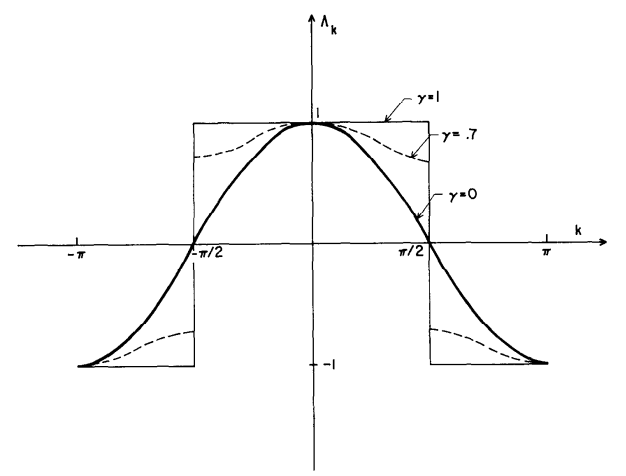
\includegraphics[scale = .75]{figs/XY_HH_model/XY_S=0.5_HH_model_energies.png}
    \caption{Energies of the elementary excitations in the $\textnormal{XY}_{S=\frac{1}{2}}$ Heisenberg model, as function of the wave vector for three different degrees of anisotropy. Retrieved from \cite{LIEB1961407}}
    \label{fig:XY_S=0.5_HH_model_energies}
\end{figure}

Consider $N$ such that $\frac{N}{4} \notin \mathds{Z}$, hence $\Lambda_k \neq 0$. Furthermore, the sign of $\Lambda_k$ is arbitrary and can be taken to be positive. This corresponds to a particle-hole picture for the $\eta$-particles, where the ground states has no elementary fermions and the fermion excitations, both above and below the Fermi surface,\footnote{\begin{tcolorbox}[colback = yellow, title = Physical Context]

The Fermi surface consists of two points, $k = \frac{\pi}{2}$. The alternate picture in which all excitations are particles, which in the isotropic case is an up-spin $\ket{\uparrow}$, can be obtained by letting $\Lambda_k$ have the sign of $\Lambda_k$. The Fermi sea would then be defined by $|k| > \frac{\pi}{2}.$ However, the particle-hole picture is preferred. 

\end{tcolorbox}} have positive energies. The energy excitations for this model can be visualized in \cref{fig:XY_S=0.5_HH_model_energies}. Only in the isotropic case $(\gamma = 0)$ there is no energy gap.\\

The ground state is defined as the state with no elementary excitations, thus 

\begin{equation}
\begin{array}{cc}
     \eta_{k} \ket{0} = 0, \blanky \forall k.  \\
     E_0 = -\frac{1}{2} \sum_{k} \Lambda_k,
     \label{XY_ccyclic_gs}
\end{array}
\end{equation}

where $E_0$ is the ground-state energy. In the thermodynamic limit, the preceding sum can be replaced by an integral, yielding 

\begin{equation}
    \begin{split}
    \frac{E_0}{N} =& -\frac{1}{4\pi} \int_{-\pi}^{\pi} dk \blanky \bigg[1 - (1-\gamma^2) \sin k \bigg] \\
    &= - \frac{1}{\pi} \mathcal{E}(1-\gamma^2),
    \begin{array}{cc}
         \textnormal{ which yields the  }  \\
         \textnormal{ following limiting cases }
    \end{array} \begin{array}{cc}
     \frac{E_0}{N} = - \frac{1}{\pi} & \textnormal{ for the isotropic case, } \gamma = 0\\ 
     \\
     \frac{E_0}{N} = - \frac{1}{2} & \textnormal{ for the Ising case, } \gamma = 1. 
\end{array}
    \end{split} 
\end{equation} 

where $\mathcal{E}(\cdot)$ is one of the complete elliptic integrals. The $\frac{E_0}{N}$-quantity is analytic and goes smoothly between the $(\gamma=0)$- and $(\gamma=1)$-limiting cases. 

\begin{tcolorbox}[colback = yellow, title = Physical Context]

The previous relations hold, in principle, only or the $c$-cyclic problem, rather than the full $a$-problem. The Hamiltonian in the $a$-cyclic term has an additional non-local term 

$$
 - \frac{1}{2} \bigg[{\bf c}_N^\dagger {\bf c}_1 + {\bf c}_1^\dagger {\bf c}_N + \gamma {\bf c}_N^\dagger {\bf c}_1^\dagger + \gamma {\bf c}_1 {\bf c}_N\bigg] (e^{i\pi \mathfrak{F}} + 1).
$$

The $\mathfrak{F}$ is not invariant under the transformations shown in \cref{XY_Jordan_Wigner}, but its evenness or oddness does remain invariant, with the same being true for $e^{i\pi \mathfrak{F}}$. 

\begin{itemize}
    \item Now, in the ground state of the $c$-cyclic problem, given by \cref{XY_ccyclic_gs}, and in all states with an even number of excitations, the number of $c$-particles is odd (check the definition of the $c$-particles in terms of the $\eta$-particles, given by \cref{XY_Hamiltonian_diag_ops}, and consider that the ground state is defined in terms of the $\eta$-particles)\footnote{assuming $\frac{N}{4} \notin \mathds{Z}$, the $k$s are occupied symmetrically around $K = 0$, except that $k = \pi$, but no $k= -\pi$, is occupied. }. Hence an additional term gives zero net difference, when acting on said states and thus, for an even number of excitations, these states remain eigenstates of the $a$-cyclic problem. \\
    \item For states with an odd number of excitations, on the other hand, $\mathfrak{F}$ is even, giving rise to an additional term, 
    
    $$
        - \frac{1}{2} \bigg({\bf c}_N^\dagger {\bf c}_1+ \gamma {\bf c}_N^\dagger{\bf c}_1 + \textnormal{h.c.} \bigg),
    $$
    
    in the Hamiltonian. This induces corrections of $\mathcal{O}(N^{-1})$ on the $k$s, the $\bm{\Phi}_k$'s and the $\bm{\Psi}_k$'s, all of which can be calculated exactly but are negligible in the calculation of physical quantities. Strictly speaking, the elementary excitations are not independent for the $a$-cyclic problem, since there is a dependence on the evenness or oddness of the total number of excitations present. 
\end{itemize}

\end{tcolorbox}

\blanky \\

The free energy is given by the grand potential of such a system of non-interacting fermions with zero chemical potential,

\begin{equation}
    \frac{F_{\gamma}}{N} = -\beta^{-1} \bigg[\alpha + \frac{2}{\pi} \int_{0}^{\frac{\pi}{2}}\ dk \blanky \log \cosh \frac{\beta \Lambda_k}{2} \bigg], \begin{array}{cc}
         \textnormal{ which yields the  }  \\
         \textnormal{ following limiting cases }
    \end{array} \begin{array}{cc}
      \frac{F_{\textnormal{isotrop.}}}{N} = -\beta^{-1} \bigg[\alpha + \frac{2}{\pi} \int_{0}^{\frac{\pi}{2}}\ dk \blanky \log \cosh \frac{\beta \cos k}{2} \bigg] & \textnormal{ for the isotropic case, } \gamma = 0\\ 
     \\
      \frac{F_{\textnormal{isotrop.}}}{N} = - \frac{\alpha + \log \cosh \frac{\beta}{2}}{\beta} & \textnormal{ for the Ising case, } \gamma = 1,
\end{array},
\end{equation}

where $\alpha = \log 2$. Neither case exhibits any singular behaviour as a function of the temperature, a result to be expected in view of the one-dimensional nature of the model. \\

\underline{Short- and long-range order in the Ground state}

The long-range order for the Heisenberg model is often defined in terms of two sublattices\footnote{In the case of a linear one-dimensional chain, these sublattices may be defined to be, one corresponding to all even sites and the other one corresponding to all odd sites.}. It is taken to be the preponderance of spins up to spins down on one of the sublattices or viceversa.

\begin{itemize}
    \item Since the Heisenberg Hamiltonian is $SU(2)$-invariant, in particular it is invariant under a rotation in $\theta^{i} = \pi, \blanky i =x,y,z$,
    \item is translationally invariant,
    \item and the ground state is non-degenerate,
\end{itemize}

then, according to this definition for long-range order, it must be zero even if the state itself was ordered. However note that the completely ferromagnetic states can have long-range order by this definition only because these are highly degenerate. This definition for long-range order, though somewhat lacking, is useful since the approximate states considered have not always had the full symmetries of the Hamiltonian.\\

A much better measure for the long-range order is the time dependent spin correlation tensor, 

\begin{equation}
    \rho_{\ell m}(t) = \bra{\Psi_0} \spin_{\ell}(0) \spin_{m}(t) \ket{\Psi_0}
\end{equation}

\clearpage

\paragraph{\textbf{$\Delta \approx 1$: The isotropic Heisenberg Antiferromagnet}}

The most interesting regime for the XXZ chain is $\Delta \approx 1$, ie. the vicinity of the Isotropic Heisenberg antiferromagnet (HAF), wherein the ground state energy is given by 

$$
    E_0 = - N J \log 2.
$$

\clearpage

\subsubsection{Antiferromagnetic Ground States}

Consider an $N$-lattice system with spin-$S$, with its Hamiltonian given by

\begin{equation}
    {\bf H} = {\bf H}^{zz} + {\bf H}^{xy}, \begin{array}{c}
         {\bf H}^{zz} = \frac{1}{2} \sum_{ij \in \Lambda \subset Z^{d}} J_{ij} \spin_i^z \spin_j^z, \\  
         \\
         {\bf H}^{xy} = \frac{1}{4} \sum_{ij \in \Lambda \subset Z^{d}} J_{ij} (\spin_i^+ \spin_j^- + \spin_i^- \spin_j^+), \\  
    \end{array}
    \label{auerbach's HH hamiltonian}
\end{equation}

with $J_{ij} = J_{ji}$ having translational symmetry. Furthermore, this Hamiltonian is rotationally invariant, having an $SU(2)$-symmetry, since it commutes with all three components of the total spin. Thus, the eigenstates may be labelled by 

\begin{equation}
    \begin{array}{c}
         \ket{\Phi} = \ket{\spin_{\textnormal{tot}}, M, \cdots},  \\
         M = -\spin_{\textnormal{tot}}, - -\spin_{\textnormal{tot}} +1, \cdots,  \spin_{\textnormal{tot}}, \\          \spin_{\textnormal{tot}} \leq NS, 
    \end{array} \begin{array}{c}
         \textnormal{ where $M$ is the eigenvalue of the total magnetization $\spin_{\textnormal{tot}}^z$,}
         \\
         \textnormal{ and where $\spin_{\textnormal{tot}}^2 = \spin_{\textnormal{tot}}(\spin_{\textnormal{tot}}+1)$ is the $SU(2)$-Casimir invariant. } \\
         \textnormal{Note that, if the model is translationally invariant} \\
         \textnormal{the ${\bf k}$-momentum is also a good quantum number.}
    \end{array}
\end{equation}

\blanky \\

The antiferromagnetic ground state is, in general, far more complicated than the ferromagnetic ground state. There are a series of theorems on the ground states, which hold for bipartite antiferromagnetic Hamiltonians. Consider two lattices, $A$ and $B$, then the staggered magnetization operator on these sublattices is given by 


\begin{equation}
    \spin^{\textnormal{stagg}} = \sum_{i \in A} \spin_{i}^z - \sum_{i \in B} \spin_{i}^z.
\end{equation}

The Ising configuration form the basis set 

$$
\prod_{i=1}^{N} \ket{S, m_{i}^\alpha}_{i} \begin{array}{c}
     \textnormal{ where $\ket{S, m_i}_i$ is an eigenstate of $\spin_i^2, \spin_i^z$ } \\
     \textnormal{ with eigenvalues $S(S+1), m_i$ respectively}.
\end{array}
$$

In this bipartite system, the Néel state maximizes the staggered magnetization and is given by the Ising configuration

\begin{align}
    \ket{\Psi^{\textnormal{{Néel}}}} &= \prod_{i=1}^{N} \ket{S, \eta_i S_i}, & \eta_i &= \left\{\begin{array}{cc}
        1 & i \in A  \\
        -1 & i \in B
    \end{array} \right.
\end{align}

Note that the Néel state may only be defined for bipartite states. Generally, this state is not an eigenstate of the Hamiltonian, since the spin flip terms $\spin_i^+ \spin_j^-$
connect the Néel state to other (non-Néel) Ising spin configurations. Now, it is convenient to rotate the spin axes on the $B$-sublattice about the $z$-axis, which amounts to the unitary transformation 

\begin{equation}\begin{array}{c}
     \spin_i^+ \rightarrow - \tilde{\spin}_i^+ \\
     \spin_i^- \rightarrow - \tilde{\spin}_i^- \\
     \spin_i^z \rightarrow + \tilde{\spin}_i^z, 
\end{array}
    \ket{S, m_i}_i \rightarrow \ket{S, \tilde{m}_i}_i = \left\{\begin{array}{cc}
        \ket{S, m_i}_i & i \in A \\
        (1-)^{S+m_i} \ket{S, m_i}_i & i \in B 
    \end{array} \right., 
    \label{HH_su2_rotation}
\end{equation}

where $\tilde{m}_i$ are eigenvalues of $\spin_i^z$ and $\tilde{\spin}_i^z$ on $A$ and $B$ sublattices, respectively. By restricting the problem to an $M$-subspace, all wave functions may be rewritten as 

\begin{equation}
    \ket{\Psi^M} = \sum_{\alpha} f_{\alpha}^M \ket{\tilde{\Psi}^M_{\alpha}}, \textnormal{ where } \ket{\tilde{\Psi}^M_{\alpha}} = \prod_{\sum_{i} \tilde{m}_i^\alpha = M} \ket{S, \tilde{m}_i^\alpha}. 
\end{equation}

Then, the following theorems, first presented by Marshall and then extended by Lieb and Mattis, arise

%\begin{tcolorbox}[title = Marshall's theorems]

\begin{theorem}
    Consider the Hamiltonian given by \cref{auerbach's HH hamiltonian}, of a bipartite lattice with antiferromagnetic exchanges $J_{ij} \geq 0$ which connect two sublattices $A$ and $B$. Said antiferromagnetic exchanges are such that any two lattice sites are connected by a sequence of finite exchanges between intermediary sites. In any allowed $M$-sector, the lowest energy state $\ket{\Psi^M_0}$ can be chosen to have positive-definite coefficients in the rotated Ising basis $\ket{\tilde{\Psi}^M_{\alpha}}$ ie.
    
    \begin{align}
        \ket{\Psi^M_0} &= \sum_{\alpha} f_{\alpha}^M \ket{\tilde{\Psi}^M_{\alpha}}, & \{f_{\alpha}^M\}_{\alpha} > 0 \\
        &= \sum_{\alpha} (-1)^{\Gamma(\alpha)} f_{\alpha}^M \ket{{\Psi}^M_{\alpha}}, & \Gamma(\alpha) = \sum_{i \in B} (S + m_i^\alpha).
    \end{align}
    \label{Marshall_theo_1}
\end{theorem}

\begin{theorem}
The absolute ground state $\ket{\Omega}$, for equal size sublattices $A$ and $B$, is a singlet of zero total spin, this is 

$$
    {\spin}_{\textnormal{tot}} \ket{\Psi^M_0}= 0.
$$
\label{Marshall_theo_2}
\end{theorem}
%\end{tcolorbox}

Note that not all total singlets obey the so-called Marshal sign criterion and, conversely, not all Marshall sign-obeying states are singlets of the total spin. The ground state of the Heisenberg Hamiltonian must, however, obey both conditions. \\

\begin{proof}

Consider an $SU(2)$-rotation, acting trivially on the first lattice and non-trivially in the second system. This is,

$$
    U \in SU(2) | U: (\mathfrak{s}\mathfrak{u}(2)_A) \times (\mathfrak{s}\mathfrak{u}(2)_B) \rightarrow (\mathfrak{s}\mathfrak{u}(2)_A) \times (\mathfrak{s}\mathfrak{u}(2)_B) \blanky \land \blanky \begin{array}{cc}
        () &  \\
         & 
    \end{array}
$$

Consider an $SU(2)-$rotation, under which the spin operators and Ising basis transform as \cref{HH_su2_rotation}. The Heisenberg Hamiltonian in this new representation then reads 

\begin{equation}
    \tilde{{\bf H}} = \tilde{{\bf H}}^{zz} + \tilde{{\bf H}}^{xy}, \begin{array}{c}
        \tilde{{\bf H}}^{zz} = \sum_{ij \in \Lambda \subset Z^{d}} |J_{ij}| \spin_i^z \tilde{\spin}_j^z, \\  
         \\
        \tilde{{\bf H}}^{xy} = - \frac{1}{2} \sum_{ij \in \Lambda \subset Z^{d}} |J_{ij}| (\spin_i^+ \tilde{\spin}_j^- + \spin_i^- \tilde{\spin}_j^+), \\  
    \end{array}
    \label{auerbach's HH hamiltonian}
\end{equation}

\begin{equation*}
    \begin{array}{cc}
    \textnormal{wherein, in this new sublattice-rotated representation,} \\
        \textnormal{the longitudinal term, $\tilde{{\bf H}}^{zz}$, is diagonal in the rotated } & \textnormal{and where the transverse $\tilde{{\bf H}}^{xy}$ has non-positive } \\
        \textnormal{Ising configuration: } \tilde{{\bf H}}^{zz}\ket{\tilde{\Psi}_{\alpha}} = e_{\alpha} \ket{\tilde{\Psi}_{\alpha}} & \textnormal{ matrix elements:} 
        \bra{\tilde{\Psi}_{\alpha}} \tilde{{\bf H}}^{xy}  \ket{\tilde{\Psi}_{\beta}} = -|K_{\alpha \beta}|. \\
    \end{array}
\end{equation*}

Both of these matrix representations induce the following eigenvalue equation on the $f$-coefficients, 

\begin{equation*}\begin{split}
    \tilde{{\bf H}} \ket{\tilde{\Psi}_{\alpha}} = E \ket{\tilde{\Psi}_{\alpha}} \Rightarrow - \sum_{\beta} |K_{\alpha \beta}| f_{\beta} + e_{\alpha} f_{\alpha} = E f_{\alpha}. \\
    \begin{array}{c}
         \textnormal{Consider then the trial function} \\
          \ket{\tilde{\Omega}} = \sum_{\alpha} |f_{\alpha}| \ket{\tilde{\Psi}_{\alpha}} \\
          \textnormal{ whose energy is }
    \end{array}
    \bra{\tilde{\Omega}} \tilde{{\bf H}} \ket{\tilde{\Omega}} &=  \sum_{\alpha} e_{\alpha} |f_{\alpha}|^2 - \sum_{\alpha \beta} |K_{\alpha \beta}| |f_{\alpha}| |f_{\beta}| \\
    & \leq \sum_{\alpha} e_{\alpha} |f_{\alpha}|^2 - \sum_{\alpha \beta} |K_{\alpha \beta}| f_{\alpha} f_{\beta} = E,
\end{split}
\end{equation*}

where the last equality holds if and only if all of the $f_{\alpha}$-coefficients are non-negative or all of the $f_{\alpha}$-coefficients are negative. This state must, therefore, also be a ground state and satisfy the eigenvalue equation 

$$
    - \sum_{\beta} |K_{\alpha \beta}| |f_{\beta}| + e_{\alpha} |f_{\alpha}| = E |f_{\alpha}|.
$$

In general, the $\ket{\tilde{\Psi}}$-states are not eigenstates of the rotated Hamiltonian, except in the case in which $M = NS$ which is the case of a one-state space. Therefore, $e_{\alpha} > E, \blanky \forall \alpha$. Then, 

\begin{equation}
    \begin{split}
    &(e_{\alpha} - E) f_{\alpha }= \sum_{\beta} |K_{\alpha \beta}| f_\beta \\
    &(e_{\alpha} - E) |f_{\alpha}|= \sum_{\beta} |K_{\alpha \beta}| |f_\beta|  
    \end{split} \Rightarrow \bigg|\sum_{\beta} |K_{\alpha \beta}| f_{\beta}\bigg| = \sum_{\beta} |K_{\alpha \beta}| |f_{\beta}| \Rightarrow f_{\beta} \geq 0.
\end{equation}

Thus, the trial state and the ground states are the same, upto phase factors: $\ket{\tilde{\Omega}} = \pm \ket{\Psi^M_0}$. An even stronger condition on the $f_{\beta}$s can be imposed.

\begin{lemma}
   $f_{\beta} > 0, \blanky \forall \beta$.
\end{lemma}

\begin{proof}
In effect, any Ising configuration with total magnetization $M$ is connected to all other configurations in the same sector by successive application of the pairwise spin flip operator ${\bf K}_{\alpha \beta} \approx (\sum_{i,j} \spin_i^+ \tilde{\spin}_j^- + \spin_i^- \tilde{\spin}_j^+)_{\alpha \beta}$. Thus, if $\exists \alpha: f_{\alpha} = 0$ , then $f_{\beta}$ must vanish for all other $\beta$ in the same $M$-sector. Since, by design, the ground state is such that in its expansions there is at least one non-zero coefficient, it follows that $f_{\beta} > 0$, $\forall{\beta}$, thus proving \cref{Marshall_theo_1}.
\end{proof}

\begin{corr}
For any fixed $M$, $\ket{\Psi^M_0}$ is non-degenerate.
\label{HH_non_degeneracy}
\end{corr}

\begin{proof}
In effect, since all $f_{\beta}$s are non-zero, there cannot be an orthogonal state to $\ket{\Omega}$ that has only positive definite coefficients in said $M$ subspace. \\
\end{proof}

For \cref{Marshall_theo_2} to hold, the ground state of the $M$-sector must have minimally possible total spin, 

\begin{lemma}
   For a bipartite antiferromagnetic Heisenberg model, 
   
   $$
   (\spin_{\textnormal{tot}})^2 \ket{\Psi^M} = M(M+1)\ket{\Psi^M}
   $$
\end{lemma}

\begin{proof}
Consider the infinite range Hamiltonian on a bipartite lattice with equal number of sites on the two sublattices, 

$$
    {\bf H}^{\infty} = J \sum_{\substack{
    i \in A \\
    j \in B}} \vec{\spin}_i \cdot \vec{\spin}_j = J \spin_{\textnormal{tot}}^A \cdot \spin_{\textnormal{tot}}^B
$$

This problem is thus trivially solvable, since it is a two spin problem using $\spin_{\textnormal{tot}} = \spin_{\textnormal{tot}}^A + \spin_{\textnormal{tot}}^B$, since $\spin_{\textnormal{tot}}^A \cdot \spin_{\textnormal{tot}}^B = \frac{1}{2} \bigg( \spin_{\textnormal{tot}}^2 - (\spin_{\textnormal{tot}}^A)^2 - (\spin_{\textnormal{tot}}^B)^2 \bigg)$.
Therefore, the possible values of the total spin operators are 

$$
    \spin_{\textnormal{tot}}^A, \spin_{\textnormal{tot}}^B = 0, 1, \cdots, \frac{NS}{2},
$$

which for equal size sublattice means that 

\begin{equation}
    0 \leq \spin_{\textnormal{tot}} \leq NS.
    \label{infinite_range_HH_total_spin}
\end{equation}

This infinite-range Hamiltonian's eigenvalues are then 

\begin{equation}
    E^{\infty} (\spin_{\textnormal{tot}}) = \frac{J}{2} \bigg[\spin_{\textnormal{tot}}(\spin_{\textnormal{tot}} + 1) - \spin_{\textnormal{tot}}^A(\spin_{\textnormal{tot}}^A+1) - \spin_{\textnormal{tot}}^B(\spin_{\textnormal{tot}}^B)\bigg],
\end{equation}

which are monotonically increasing with $\spin_{\textnormal{tot}}$, and since $\spin_{\textnormal{tot}} > M$, the ground state in a given $M$-sector has 

$$
\spin_{\textnormal{tot}} = M.
$$

Now, note that both the Heisenberg Hamiltonian and the infinite range Hamiltonian satisfy the requirements for the first of Marshall's theorems, \cref{Marshall_theo_1}, and thus their ground states have Marshall signs. Therefore, their overlap is non-zero, since it involves a sum over positive number, and these must have the same total spin quantum numbers. Therefore, the lowest energy state of ${\bf H}$ in the $M$-sector has spin $\spin_{\textnormal{tot}} = M$. Since all allowed values of total spin $\spin_{\textnormal{tot}}' > M$ have members in the sector with magnetization $M$, then the energy in terms of the total spin obeys 

$$
    \forall \spin_{\textnormal{tot}}' > \spin_{\textnormal{tot}} \Rightarrow E(\spin_{\textnormal{tot}}') > E(\spin_{\textnormal{tot}}),
$$

ie. the energy is a monotonically increasing function of the total spin. Now, consider the $(M=0)$-sector. This inequality proves that the ground state must have minimal possible total spin $\spin_{\textnormal{tot}}$ which is zero, according to \cref{infinite_range_HH_total_spin}. Thus concluding the proof of \cref{Marshall_theo_2}.
\end{proof}
\end{proof}

\subsubsection{Ferromagnetic Ground States}

For the ferromagnetic Heisenberg chains, a similar result can be proved. 

\begin{corr}
For the ferromagnetic model with non-positive charges, 

$$
{\bf H} = - \frac{1}{2} \sum_{ij} |J_{ij}| \vec{\spin}_i \cdot \vec{\spin}_j,
$$

the fully ferromagnetic state $\ket{\Psi^{\textnormal{FM}}}$ is a member of the ground state multiplet, where 

$$
    \ket{\Psi_0^{\textnormal{FM}}} = \prod_{i=1}^N \ket{S, S}_i.
$$

\end{corr}

\begin{proof}

Consider the ferromagnetic Heisenberg model, whose Hamiltonian may be explicitly written as 

\begin{equation}
     {\bf H} = {\bf H}^{zz} + {\bf H}^{xy}, \begin{array}{c}
         {\bf H}^{zz} = -\frac{1}{2} \sum_{ij \in \Lambda \subset \mathds{Z}^{2}} |J_{ij}| \spin_i^z \spin_j^z, \\  
         \\
         {\bf H}^{xy} = -\frac{1}{4} \sum_{ij \in \Lambda \subset \mathds{Z}^{2}} |J_{ij}| (\spin_i^+ \spin_j^- + \spin_i^- \spin_j^+). \\  
    \end{array}
\end{equation}

For a fixed $M$-subspace, all wave functions may be written in terms of Ising configurations which lie in said $M$-subspace, namely

\begin{equation}
    \ket{\Psi^M} = \sum_{\alpha} f_{\alpha}^M \ket{{\Psi}^M_{\alpha}}, \textnormal{ where } \ket{{\Psi}^M_{\alpha}} = \prod_{\sum_{i} {m}_i^\alpha = M} \ket{S, {m}_i^\alpha}. 
\end{equation}

Now, 

\begin{itemize}
    \item the longitudinal term, ${{\bf H}}^{zz}$, is diagonal in the Ising configurations, ${{\bf H}}^{zz}\ket{{\Psi}_{\alpha}} = e_{\alpha} \ket{{\Psi}_{\alpha}}$,
    \item and where the transverse ${{\bf H}}^{xy}$ has non-negative $\bra{{\Psi}_{\alpha}} {{\bf H}}^{xy}  \ket{{\Psi}_{\beta}} = |K_{\alpha \beta}|$.
\end{itemize}

Consider the following ansatz, $\ket{\Omega} = \sum_{\alpha} |f_{\alpha}| \ket{\Psi}_{\alpha}$, whose energy is 

\begin{equation}
\begin{split}
    \bra{\Omega} H \ket{\Omega} = & \sum_{\alpha} e_{\alpha} |f_{\alpha}|^2 + \sum_{\alpha \beta} |K_{\alpha \beta}| |f_{\alpha}| |f_{\beta}| \\
    & \leq \sum_{\alpha} e_{\alpha} |f_{\alpha}|^2 + \sum_{\alpha \beta} |K_{\alpha \beta}| f_{\alpha} f_{\beta} = E \Rightarrow \textnormal{sgn}(f_{\alpha}) = \textnormal{sgn}(f_{\beta}), \forall \alpha, \beta. 
\end{split}
\end{equation}

Without loss of generality, the $f_{\alpha}$-coefficients may be taken to be positive, with the extra, overall, sign to be associated with the Ising configurations. In effect, in general, the $\ket{{\Psi}}$-states are not  eigenstates of the Hamiltonian, except in the case in which $M = NS$ which is the case of a one-state space. Therefore, $e_{\alpha} > E, \blanky \forall \alpha$.
Consider the infinite range ferromagnetic Hamiltonian on a bipartite lattice with equal number of sites on the two sublattices, 

$$
    {\bf H}^{\infty} = -J \sum_{\substack{
    i \in A \\
    j \in B}} \vec{\spin}_i \cdot \vec{\spin}_j = -J \spin_{\textnormal{tot}}^A \cdot \spin_{\textnormal{tot}}^B
$$

Again, this problem is trivially solvable, since it is a two spin problem using $\spin_{\textnormal{tot}} = \spin_{\textnormal{tot}}^A + \spin_{\textnormal{tot}}^B$, since $\spin_{\textnormal{tot}}^A \cdot \spin_{\textnormal{tot}}^B = \frac{1}{2} \bigg( \spin_{\textnormal{tot}}^2 - (\spin_{\textnormal{tot}}^A)^2 - (\spin_{\textnormal{tot}}^B)^2 \bigg)$.
Therefore, the possible values of the total spin operators are 

$$
    \spin_{\textnormal{tot}}^A, \spin_{\textnormal{tot}}^B = 0, 1, \cdots, \frac{NS}{2},
$$

which for equal size sublattice means that 

\begin{equation}
    0 \leq \spin_{\textnormal{tot}} \leq NS.
    \label{infinite_range_HH_total_spin}
\end{equation}

This infinite-range Hamiltonian's eigenvalues are then 

\begin{equation}
    E^{\infty} (\spin_{\textnormal{tot}}) = -\frac{J}{2} \bigg[\spin_{\textnormal{tot}}(\spin_{\textnormal{tot}} + 1) - \spin_{\textnormal{tot}}^A(\spin_{\textnormal{tot}}^A+1) - \spin_{\textnormal{tot}}^B(\spin_{\textnormal{tot}}^B)\bigg],
\end{equation}

which are monotonically increasing with $\spin_{\textnormal{tot}}$, and since $\spin_{\textnormal{tot}} > M$, the ground state in a given $M$-sector has 

$$
\spin_{\textnormal{tot}} = M.
$$
\end{proof}

As a member of a degenerate multiplet, this state spontaneously breaks the rotational symmetry of the Hamiltonian. This symmetry breaking is special in that the operator $\spin_{\textnormal{tot}}^z$ commutes with the Hamiltonian and, therefore, $M$ is a good quantum number (ie. it labels the eigenstates of ${\bf H}$). In this respect, the antiferromagnet differs from the ferromagnet. The staggered magnetization does not commute in general with the Hamiltonian. Spontaneous symmetry breaking, however, is still possible for the antiferromagnet in the strict thermodynamic limit. \\

\subsubsection{Half-Odd Integer Spin Chains}

As a Lie group, $SU(2)$ is the simply-convex three-sphere $\bm{\mathcal{S}}^3$. Thus, particle with half-odd integer spin, eg. electrons, have a peculiar quantum property: their wave functions acquires a minus sign under a $2\pi$-rotation about any spin axis. For localized systems, any particular direction in spin space, this effect is not noticeable. However, for low-dimensional systems, this zero-point fluctuations are large. Thus, interference effects due to these negative signs may become important. In fact, the antiferromagnetic one-dimensional Heisenberg model has different spectra for integer and half-odd integer spins. Thus the following theorem, due to Lieb, Schultz and Mattis, arises:

%\begin{tcolorbox}[title = Lieb-Schultz-Mattis Theorem on Half-odd Integer Spin Chains]

\begin{theorem} \textbf{\textnormal{Lieb-Schultz-Mattis Theorem on Half-odd Integer Spin Chains.}} 
Consider the antiferromagnetic Heisenberg spin chain, with $J > 0$ on a one dimensional chain with closed topology 

\begin{equation}
    {\bf H} = J \sum_{j=1}^N \spin_j \cdot \spin_{j+1} + J \spin_N \cdot \spin_1,
\end{equation}

where $N$ is even. For half-odd integer spin, there exists an excited state whose energy vanishes in the thermodynamic limit, $N \rightarrow \infty$.
\end{theorem}
%\end{tcolorbox}

Let $\ket{\Psi_0}$ be the system's ground state and let the twist operator be 

$$
    \mathcal{O}^k = \exp \bigg(ik \sum_{j=1}^{N} j \spin_j^z\bigg),
$$

which incrementally rotates each spin in the $xy$-plane, such that between the first and last spin, the spin coordinates are rotated by $2\pi$ about the $z$-axis. Thus, the twisted state is constructed as 
$$
    \ket{\Psi_k} = \mathcal{O}^k \ket{\Psi_0}
$$

Two statements swiftly arise, 

\begin{lemma}
\label{HH_1_dimensional_twisted_state}
   \begin{equation}
       \bra{\Psi_k} \ket{\Psi_0} = 0 \textnormal{ and } \bigg[\bra{\Psi_k} {{\bf H}} \ket{\Psi_k} - E_0\bigg] \underset{N \rightarrow \infty}{\rightarrow} 0
 \end{equation}
\end{lemma}

\begin{proof}
In effect, consider a translation operator, defined by cyclically shifting the spins by one site modulo $N$, this is 

\begin{equation}
\begin{split}
    &\mathcal{T} : \mathfrak{A}_i \rightarrow \mathfrak{A}_j \\
    &\mathcal{T}^{-1} \vec{\bf S}_i \mathcal{T} = \vec{\spin}_{i+1}
\end{split}
\begin{array}{c}
     \textnormal{ where } \mathfrak{A}_i, \mathfrak{A}_j \simeq \mathfrak{su}(2) \blanky \forall i,j. 
\end{array}
\end{equation}

By construction, the Heisenberg Hamiltonian with closed boundary conditions commutes with the translation operator, $[{\bf H}, \mathcal{T}] = 0$.
Then, if $\ket{\Psi_0}$ is an eigenstate of the Hamiltonian, so is $\mathcal{T} \ket{\Psi_0}$. Given $\ket{\Psi_0}$'s non-degeneracy, and guaranteed by \cref{HH_non_degeneracy}, and letting $k_0$ be the ground state lattice momentum, the following holds

\begin{equation}
\begin{split}
    \mathcal{T} \ket{\Psi_0} = e^{i k_0} \ket{\Psi_0} 
    \Rightarrow \bra{\Psi_0} \ket{\Psi_k} &= \bra{\Psi_0} \mathcal{O}^{k}\ket{\Psi_0} =  \bra{\Psi_0} \mathcal{T}^{-1} \mathcal{O}^{k} \mathcal{T} \ket{\Psi_0} \\
    &= \bra{\Psi_0} \exp \bigg[-ikN \sum_{j=1}^{N} j \mathcal{T}^{-1} \spin_j^z \mathcal{T} \bigg] \ket{\Psi_0} \\
    &= \bra{\Psi_0} \exp \bigg[-ikN \bigg( \sum_{j=1}^{N-1} j \spin_{j+1}^z + N \spin_1^z \bigg)\bigg) \ket{\Psi_0} \\
    &= \bra{\Psi_0} e^{i k N  \spin_1^z}\exp \bigg[-ikN \bigg( \sum_{j=1}^{N-1} (j+1) \spin_{j+1}^z + \spin_{1}^z - \sum_{j=1}^{N}  \spin_{j+1}^z  \bigg)\bigg] \ket{\Psi_0} \\
    &= \bra{\Psi_0} e^{i k N \spin_1^z} \exp \bigg(-ikN \bigg( \sum_{j=1}^{N} (j+1) \spin_{j+1}^z - \sum_{j=1}^{N}  \spin_{j+1}^z  \bigg)\bigg] \ket{\Psi_0} \\
    &= \bra{\Psi_0} e^{i 2 \pi \spin_1^z} \mathcal{O}^k  \exp \bigg(- i k N \spin_{\textnormal{tot}}^z\bigg) \ket{\Psi_0} \\
    &= \bra{\Psi_0} \mathcal{O}^{k} e^{ik \spin_1^z} \exp \bigg(-ikN \sum_{j=1}^{N} j \spin_j^z \bigg) \ket{\Psi_0} \\
\end{split}
\end{equation}

This last equality is, in fact, zero by \cref{Marshall_theo_2}, the ground state has zero-total magnetization. Given that $\ket{\Psi_0}$ is a singlet, note that 

\begin{equation}
\begin{split}
    {\bf S}_1^z &= \left(\begin{array}{cc}
        \frac{1}{2} & 0  \\
        0 & -\frac{1}{2} 
    \end{array}\right) \Rightarrow \begin{array}{c}
        e^{ik \spin_1^z}  = \left\{  \begin{array}{cc}
              1 &  S = 0,1,2,\cdots \\
              -1 &  S = \frac{1}{2},\frac{3}{2},\frac{5}{2},
          \end{array} \right.
    \end{array} \Rightarrow \mathcal{T}^{-1} \mathcal{O}^{k} \mathcal{T} = \left\{  \begin{array}{cc}
              \mathcal{O}^{k} &  S = 0,1,2,\cdots \\
              -\mathcal{O}^{k} &  S = \frac{1}{2},\frac{3}{2},\frac{5}{2},
          \end{array} \right.
\end{split}
\end{equation}

which then implies that $\bra{\Psi_0} \ket{\Psi_k} = - \bra{\Psi_0} \ket{\Psi_k} = 0$, thus proving the first proposition. The $\ket{\Psi_k}$-state energies are also readily calculated. In effect, given that the twist operator is a unitary rotation on the $xy$-plane, the following results arise 

\begin{equation}
\begin{split}
     &\mathcal{O}^{k-1} \spin^x_n \mathcal{O}^{k} = \cos kn \spin_n^x + \sin kn \spin_n^y  \\
     &\mathcal{O}^{k-1} \spin^y_n \mathcal{O}^{k} = \cos kn \spin_n^y - \sin kn \spin_n^x  \\
     &\mathcal{O}^{k-1} \spin^z_n \mathcal{O}^{k} = \spin^z_n \\
     \Rightarrow \bra{\Psi_k} {{\bf H}} \ket{\Psi_k} = & \bra{\Psi_0} \mathcal{O}^{k-1} {{\bf H}} \mathcal{O}^{k} \ket{\Psi_0} = \bra{\Psi_0} \mathcal{O}^{k-1} {{\bf H}} \mathcal{O}^{k} \ket{\Psi_0} \\
     &= \bra{\Psi_0} \mathcal{O}^{k-1} \bigg( \frac{J}{2} \sum_{j \in \Lambda} \bigg(\spin_j^x \spin_{j+1}^x + \spin_j^y \spin_{j+1}^y + \spin_j^z \spin_{j+1}^z \bigg) \bigg) \mathcal{O}^{k} \ket{\Psi_0} \\
     &= E_0 + \bra{\Psi_0} [\cos k - 1] \sum_{j=1}^N (\spin_j^x \spin_{j+1}^x + \spin_j^y \spin_{j+1}^y) + \sin k \sum_{j=1}^N (\spin_j^x \spin_{j+1}^y - \spin_j^y \spin_{j+1}^x) \ket{\Psi_0}, \\
\end{split} 
\end{equation}

examining each term in the previous equation yields the following approximations

\begin{equation}
    \begin{array}{cc}
     \Rightarrow [\cos k - 1] \bra{\Psi_0} \sum_{j=1}^N (\spin_j^x \spin_{j+1}^x + \spin_j^y \spin_{j+1}^y) \ket{\Psi_0} &  + \sin k \sum_{j=1}^N (\spin_j^x \spin_{j+1}^y - \spin_j^y \spin_{j+1}^x) \\
     \blanky \blanky \blanky \blanky \blanky \blanky \blanky \blanky = \bigg[-\frac{1}{2} \bigg(\frac{2\pi}{N}\bigg)^2 - \mathcal{O}(N^{-4})\bigg] \bra{\Psi_0} \sum_{j=1}^N (\spin_j^x \spin_{j+1}^x + \spin_j^y \spin_{j+1}^y) \ket{\Psi_0} & \blanky \blanky = -i \sin k \bra{\Psi_0} [\sum_{j} j \spin_j^z, {\bf H}]\ket{\Psi_0} \\
     \leq \bigg(\frac{2\pi}{N}\bigg)^2 \frac{N}{2} + \mathcal{O}(N^{-3}) & = 0
    \end{array}
\end{equation}

Thus, for $k = \frac{2\pi}{N}$, 

$$
    \bra{\Psi_k} {{\bf H}} \ket{\Psi_k} \leq E_0 + \frac{2\pi^2}{N},
$$

and then, there is no energy gap in the thermodynamic limit. Thus concluding \cref{HH_1_dimensional_twisted_state}'s proof.  
\end{proof}

However, note that in the thermodynamic limit, the admixture of the ground state and this low-lying excited state may break a symmetry of the Hamiltonian. This is the case for the ground state and the first excited state of the Majumdar-Gosh model, which are superpositions of dimer configurations, break lattice symmetry. An alternative scenario occurs in the nearest-neighbour Heisenberg model of spin half. dess Cloizeaux and Pearson have found that magnon excitations are gappless, said excitations not being spin waves since they are not small fluctuations about a ground state with broken spin symmetry. In contrast to spin-half chains, integer spin chains have a gap in the excitation spectrum, the Haldane gap. \\

The previous results can be readily extended to two and three-dimensional lattices. In effect, for the former, consider a square lattice of $N$ sites in the $x$-direction and $M \sim \mathcal{O}(N^\nu)$ sites in the $y$-direction, where $\nu \in \mathds{R}_{[0,1]}$, with a cyclic Hamiltonian, ie.

$$
\spin_{n, M+1} = \spin_{n, 1} \textnormal{ and } \spin_{N+1, m} = \spin_{1, m},
$$

ie. the lattice is wrapped on a two-dimensional torus $\mathds{T}^2$. Let the two-dimensional twisted operator  $\mathcal{O}^k$ be 

$$
    \mathcal{O}^k = \exp\bigg(ik \sum_{n, m} n \spin_{n, m}^z \bigg),
$$

which twists the $x$-direction sites by the same amount and the $y$-direction sites by another amount. The $\ket{\Psi_k}$-states construction and orthonormality follow directly from the one-dimensional case. In this case, there is no energy gap in the continuum limit,  

$$
    \bra{\Psi_k} {{\bf H}} \ket{\Psi_k} \leq E_0 + \frac{2\pi^2}{N^{1-\nu}}.
$$

Since the excitacion energy of exact low-lying states should not depend on the shape of the entire lattice, there should be no energy gap for an $(N \times N)$-lattice either. The $\ket{\Psi_k}$ state is, unfortunately, not sufficiently like an exact low-lying excited state to give this result. A similar extension to three-dimensional lattices swiftly follows. \\

\subsection{Numerical solution to Fermionic models}

Consider a Hamiltonian describing a fermionic system, given by 

\begin{equation}
    {\bf H} = J \summation (f_{j}^{\dagger}f_{j+1} + f_{j+1}^{\dagger}f_{j}) + \sum_{j=1} \lambda_j f_{j}^{\dagger} f_j, \begin{array}{c}
         \textnormal{with the usual } \\
         \textnormal{ conmutation rules} 
    \end{array}
    \begin{array}{c}
         \{f_j, f_k\} = \{f_j^\dagger, f_k^\dagger\} = 0  \\
         \{f_j, f_k^\dagger\} = \delta_{jk}
    \end{array}
    \label{fermionic hamiltonian}
\end{equation}

where $L$ indicates the number of lattice sites, $J$ is the hopping strength, which could be either positive or negative, and where $\lambda_j$ is the on-site potential strength\footnote{The $\lambda_j$-term frequently appears in many condensed matter models, with different numerical values and interpretations, eg.

\begin{itemize}
    \item In the XX model, $\lambda_j = \lambda \blanky \forall j$. 
    \item While for the Anderson model $\lambda_j \in \mathcal{U}_{\R_{[-W, W]}}$, a uniform random variable, with $W$ being the disorder strength. 
    \item In the Aubry-André model, $\lambda_j = \lambda \cos(2\pi\sigma j)$, with $\sigma \in \mathds{I}$ and $\lambda$ quantifying the disorder strength. 
\end{itemize}}. Said Hamiltonian has open boundaries conditions since there is no hopping term across the boundary. Note that we can rewrite \eqref{fermionic hamiltonian} as 

\begin{equation}
    {\bf H} = \sum_{i, j = 1}^{L} \M_{ij} f_i^{\dagger} f_j \textnormal{ with } \begin{array}{c}
         \M \in \textnormal{GL}(L, \R), \\
         \M_{ij} = \left\{\begin{array}{cc}
             \lambda_i & \textnormal{ if } i=j  \\
              J & \textnormal{ if } j=i+1 \textnormal{ or } i = j + 1 \\
              0 & \textnormal{ otherwise}
         \end{array} \right.
    \end{array},
\end{equation}

which is a positive-defined tri-diagonal matrix.
Let ${\bf f} = (f_1 \blanky f_2 \blanky \cdots f_L)\transpose$ be a vector of the $L$ fermionic operators. Then, \eqref{fermionic hamiltonian} can be rewritten as 

\begin{align}
    {\bf H} = {\bf f}^\dagger \M {\bf f}.
\end{align}

Since $\M$ is symmetric, then it can be diagonalized  $\M = A \mathcal{D} A\transpose$, where $A \in \mathds{R}^{L \times L}$ is a real orthogonal matrix and with $\mathcal{D}_{ij} \in \mathds{R}^{L \times L} \blanky | \blanky \mathcal{D}_{ij}  = \epsilon_i \delta_{ij}$. In this context, the $A$-matrix acts on the fermionic operator as a Bogoliubov transformation, allowing for \eqref{fermionic hamiltonian} to be rewritten as 

\begin{equation}
     {\bf H} = {\bf f}^\dagger A \mathcal{D} A\transpose {\bf f} = {\bf d}^\dagger \mathcal{D} {\bf d}
     \label{fermionic matrix hamiltonian}
\end{equation}

where ${\bf d} = A\transpose {\bf f}$. Since the $A$-matrix is orthogonal, the new $d_k$-operators are fermionic operators as well, satisfying \eqref{fermionic hamiltonian}'s anti-commutation rules. Then, the new fermionic operators are 

\begin{equation*}
    \begin{array}{c}
         d_k = \sum_{j=1}^{L} A_{jk} f_j  \\ 
         \\
         f_j = \sum_{k=1}^{L} A_{jk} d_k 
    \end{array} \textnormal{ since } A\transpose A = \sum_{j,k = 1}^{L} A_{jk} A_{kj} = \mathds{1}_{L}.
\end{equation*}

Then, we can expand \eqref{fermionic matrix hamiltonian} in terms of the lattices, as follows 

\begin{equation}
    {\bf H} = \sum_{k = 1}^{L} \epsilon_k d_k^\dagger d_k,
\end{equation}

which is a sum of number operators with potentials. The eigenstates can then be constructed from the the theory's vacuum state, by applying the $d_k^{\dagger}$-fermionic operators. In the Heisenberg-picture, the $d_k$-operators can be evolved via the Heisenberg equation of motion

\begin{equation}
\frac{d}{dt} d_k = i [{\bf H}, d_k],
\label{H eom}
\end{equation}

and using that $d_k^2 = 0$, it turns out that \eqref{H eom}'s solution is simply $d_k(t) = e^{-i\epsilon_k t} d_k$. The system's correlation can be easily found by analyzing the following matrix. Let $\mathcal{N}_{jk} = \langle d_j^\dagger d_k \rangle$, where the expectation value is taken via calculating the operator's trace along the Fock space, which takes the following values 

\begin{equation}
    \mathcal{N}_{jk} = \langle d_j^\dagger d_k \rangle = \left\{\begin{array}{c}
        0 \textnormal{ or } 1 \textnormal{ if } j=k  \\
        0 \textnormal{ if } j \neq k 
    \end{array} \right.,
\end{equation}

ie. different lattice-sites are not correlated and there can only be a single fermion at most per lattice site, in accordance with Pauli's principle. A ground state, for example, would choose to turn on all fermions in the eigenmode $d$-space such that $\epsilon_k < 0$. If instead, the expectation value is taken with thermal states, the Fermi-Dirac distribution is returned, 

\begin{equation}
    \mathcal{N}_{jk} = \langle d_j^\dagger d_k \rangle_{\textnormal{th}} =  \frac{1}{1+e^{\beta \epsilon_k + \mu}} \delta_{jk}.
\end{equation}

Another interesting quality is a system with an initial configuration where the system's initial state, in real space, is known. In this setting, $\mathcal{N}_{jk}$ is known for all lattices. Consider for example the Anderson model, where the system's initial state is given by a single tensor product of $n$-fermionic states in real space, with $n<L$. Then, for all lattice sites, we have that $\N_{jj}$ is either zero or one. The $\N_{jk}$-matrix entries can then be evaluated as 

\begin{align*}
    \langle d_j^\dagger d_k \rangle = \sum_{i,j = 1}^{n < L} A_{ik} A_{jl} \langle f_i^\dagger f_j \rangle = \sum_{j=1} A_{jk} A_{jl} \langle f_j^\dagger f_j \rangle,
    \label{real system correlations}
\end{align*}

which can then be numerically computed to obtain the LHS expectation value. In general, this $\N_{jk}$-matrix will not be diagonal, which is reasonable since the system's real configuration is not an eigenstate. In principle and in practice, by inverting \eqref{real system correlations}, we can evolve any number operator or two-body correlation operator, ie.

\begin{align}
    \langle f_j^\dagger f_k \rangle = \sum_{k,l =1}^{n} A_{jk} A_{jl} \langle d_k^\dagger d_l \rangle.
\end{align}

This quantities' time evolution can then be found out to be 

\begin{equation}
    \langle f_j^\dagger(t) f_k(t) \rangle = \sum_{k,l =1}^{L} e^{i(\epsilon_k - \epsilon_l)t}A_{jk} A_{jl} \langle d_k^\dagger d_l \rangle,
\end{equation}

which can then be numerically solved. 

\clearpage 

%\section{Independent Electrons and Static Crystals}

%\subsection{Crystal lattices} 

%The mathematical concept which best describes an actual crystal lattice is that of a Bravais lattice, defined as a set of mathematical points corresponding to the discrete positions in space given by 

%\begin{equation}
 %   \{\Rb \in \R^{3} \blanky | \blanky \R = \sum_{i=1}^{3} n_i {\bf a}_i \textnormal{ with } n_i \in \mathds{Z}\},
%\end{equation}
    
%where the $\{a_i\}$-vector are the so-called primitive vector. The Bravais lattice is invariant under the operation 

%$$
%\Rb \rightarrow \Rb + {\bf T} \textnormal{ where } {\bf %T} = \sum_{i=1}^{3} L_i {\bf a}_i \blanky | \blanky L_i %\in \mathds{Z}
%

\clearpage 


\paragraph{\textbf{Ferromagnets and antiferromagnets}}

Unless geometric frustration is present, in classical systems, there is no significant difference between ferromagnets and antiferromagnets. Eg, with NN-interaction, geometric frustration occurs for lattices that are not bipartite. In a bipartite lattice, the sites can be divided into two sub-lattices such that nearest neighbours always belong to different sub-lattices. A nearest-neighbour antiferromagnetic interaction in a classical model on a bipartite lattice can typically be changed into a ferromagnetic one, by redefining the spin via a flip on all sites on one of the sub-lattices but not on the other (eg. $\uparrow \rightarrow \downarrow$ in the Ising model). The physics of such classical antiferromagnets is therefore essentially equivalent to that of the ferromagnets. \\

Antiferromagnetic quantum systems on non-bipartite lattices also exhibit interesting behaviour. But the interesting thing is that on bipartite lattices, there are a number of important differences between quantum ferromagnets and antiferromagnets. \\

\paragraph{\textbf{Quantum Ferromagnets}}

Consider the Heisenberg interaction $-J \vec{\spin}_1 \cdot \vec{\spin}_2$ across a single bond. For spin-$\frac{1}{2}$ particles, this is a simple $4 \times 4$-matrix acting on the computational basis $\mathcal{B} = \{\ket{\uparrow\uparrow}, \ket{\uparrow \downarrow}, \ket{\downarrow \uparrow}, \ket{\downarrow\downarrow}\}$, yielding 

\begin{equation*} \vec{\spin}_1 \cdot \vec{\spin}_2 = \frac{1}{4} \left(\begin{array}{*{11}c}1 & 0 & 0 & 0 \\0 & -1 & 4 & 0 \\0 & 4 & -1 & 0\\0 & 0 & 0 & 1\\\end{array}\right)\end{equation*}

Diagonalizing this matrix will yield its eigenvalues and its eigenvectors. Given the Clebsh-Gordan decomposition rule $\frac{1}{2} \otimes \frac{1}{2} = 0 \oplus 1$, these eigenvectors can be grouped into the $s=1$-triplet representation and the $s=0$-singlet representation. In effect,

\begin{equation}
    \begin{split}
        \textnormal{triplet}: \ket{\uparrow \uparrow}, \frac{1}{\sqrt{2}} \bigg(\ket{\downarrow \uparrow} + \ket{\uparrow\downarrow}\bigg), \ket{\downarrow\downarrow}, \textnormal{ with } \lambda_i = -\frac{J}{4} \\
        \textnormal{singlet}: \frac{1}{\sqrt{2}} \bigg(\ket{\downarrow \uparrow} - \ket{\uparrow\downarrow}\bigg), \textnormal{ with } \mu_i = +\frac{J}{4}
    \end{split}
\end{equation}

It is simple to check that ${\bf K} = s(s+1)$ in both cases, and that while the singlet is annihilated by all three generators $\vec{\bf S}$, acting with ${\bf S}^+$ and ${\bf S}^-$ takes members of the triplet to each other. One important difference between the ferromagnetic ($J > 0$) and the antiferromagnetic ($J < 0$) models now arises,

\begin{itemize}
    \item if $J>0$, there are multiple ground states for the ferromagnet, each member of the triplet having minimum energy $-J$,
    \item but if $J<0$, the antiferromagnetic ground state, the singlet, is unique. Moreover, the antiferromagnetic ground state is invariant under the $SU(2)$-symmetry, whereas the ferromagnetic ground states are not. \\
\end{itemize}

Additional insight comes from solving the Heisenberg model on a four-site chain, with its Hilbert space being 16-dimensional, by exploiting the model's inner symmetries. The magnetization operator ${\bf M}^z$ commutes with the Hamiltonian, which makes them simultaneously diagonalizable. For perioidic boundary conditions, the translational invariance plays a powerful role. The translation operator is defined by shifting the spins by one site modulo $N$, this is 
\begin{equation}
\begin{split}
    \mathcal{T} : \mathfrak{A}_i \rightarrow \mathfrak{A}_j \\
    \mathcal{T}^{-1} \vec{\bf S}_i \mathcal{T} = \vec{\spin}_{i+1}
\end{split}
\begin{array}{c}
     \textnormal{ where } \mathfrak{A}_i, \mathfrak{A}_j \simeq \mathfrak{su}(2) \blanky \forall i,j. 
\end{array}
\end{equation}

The Hamiltonian commutes with the translation operator when the boundary conditions are periodic, and commutes with the magnetization as well. Thus the Hamiltonian can be broken into blocks acting on states with a fixed eigenvalue of the traslation operator and of the magnetization. \\

Since $\mathcal{T}^N = \mathds{1}$ for an $N$-site chain, the eigenvalues of $\mathcal{T}$ are $\lambda_i = e^{\frac{2\pi i n}{N}}, \forall n \in \mathds{Z}$, from which the corresponding momentum can be defined as $k = \frac{2\pi n}{N}$. Then, the following holds 
$$
    \sum_{n \in \mathds{Z}_{[0, N-1]}} e^{-\frac{2\pi i n}{N}} \mathcal{T}^n \ket{s} = \ket{s} + e^{-\frac{2\pi i}{N}} \ket{s} + \cdots + e^{-\frac{2\pi i (N-1)}{N}}\mathcal{T}^{N-1} \ket{s}.
$$

For example, for a four-site chain, the translational invariance diagonalizes the enire Hamiltonian save for $m=0$ and $k = 0$ or $k = \pi$, since the corresponding eigenstates are 

\begin{equation}
    \begin{split}
        \ket{A} = \frac{1}{\sqrt{2}} \bigg({\uparrow\downarrow\uparrow\downarrow} + e^{-i\pi k} {\downarrow\uparrow\downarrow\uparrow}\bigg), \\
        \ket{B} = \frac{1}{2}  \bigg(\ket{{\uparrow\uparrow\downarrow\downarrow}} + \ket{\downarrow \uparrow \uparrow \downarrow} + \cdots \bigg)
    \end{split} \begin{array}{c}
         \textnormal{with the hamiltonian} \\ \textnormal{ on these} \\ \textnormal{ $k=0$ and $k=\pi$} \\ \textnormal{states being }  
    \end{array}-J \left(\begin{array}{cc}
        -1 & \sqrt{2} \cos\left(\frac{\pi k}{2}\right)  \\
        \sqrt{2} \cos\left(\frac{\pi k}{2}\right) & 0
    \end{array}\right).
\end{equation}

These sector's eigenvalues are therefore $-J$ and $2J$ for $k=0$ and $J = 0$ for $k=\pi$. Again organising the eigenstates into $\mathfrak{su}(2)$-multiplets yield the energy levels divided by $-J$, as follows 

\begin{equation}
    \begin{split}
        & \textnormal{quintuplet}: 1 \\
        & \textnormal{triplets}: \cos(\pi k) (k \neq 0) \\
        & \textnormal{singlets}: -2,0 \textnormal{ for } k=0, \pi \textnormal{ respectively}. 
    \end{split}
\end{equation}

This $\mathfrak{su}(2)$-invariance allows for the construction of the entire multiplet once one of the states is known. \\

As with the two-site chain, the ferromagnetic ground state is a multiplet, whereas the antiferromagnetic is a singlet. For a general $N$-site ferromagnet, the completely ferromagnetic states (all spins up or all spins down) are exact ground states of the Hamiltonian. This suggest using an order parameter for ferromagnetism. A ferromagnetic order parameter is simply the quantum analog of the magnetization, the expectation value of the $z$-component of the total spin is 

$$
    \bra{\textnormal{g.s.}} {\bf M}^z \ket{\textnormal{g.s.}} = \sum_{i=1}^N \textnormal{g.s.} \bra{\textnormal{g.s.}} {\bf S}_i^z \ket{\textnormal{g.s.}},
$$

which is not a particularly great order parameter, since it vanishes if there is symmetry under spin flip, as with the classical case. A better example is $\bra{\textnormal{g.s.}} ({\bf M}^z)^2 \ket{\textnormal{g.s.}}$. \\

The completely ferromagnetically ordered states, ie. all spins up or all spins down, are both ${\bf M}^z$-eigenvalues with maximum magnitude of eigenvalues, namely $N^2$, and are ground states of the Hamiltonian as well. The antiferromagnetic situtation is different. The staggered magnetization, or the \textbf{Néel order parameter}, is commonly used to understand antiferromagnetic order. It can only be defined on bipartite lattices. For example, consider the odd-sites on a sublattice, and the even-sites on the other, then the Néel operator is 

$$
    \bm{\mathcal N} = \sum_{i=1}^N (-1)^i {\bf S}_i^z.
$$

A Néel state has $N^2$-eigenvalues under $\bm{\mathcal N}^2$, ie. the spins are spin up on one sublattice and spin down on the other, like the state $\ket{A}$ which has four sites. Note, however, that the Néel operator does not commute with Hamiltonian. Then, a Néel state is not an eigenstate of the Heisenberg Hamiltonian. This is a huge difference between ferromagnets and antiferromagnets, even on bipartite lattices, not just on geometrically frustrated ones. 

For example, for a four-site chain and $J<0$, the ground state is a spin singlet and translationally invariant. The properties are thus quite typical of antiferromagnetic ground states. The diagonal terms are $J$ and $0$ for the translationally-invariant Néel state $\ket{A}$ and the other state, $\ket{B}$, respectively. This does indeed favour the Néel state. However, the off-diagonal terms in the Hamiltonian, mean \\

\clearpage

\paragraph{\textbf{Hamiltonian in terms of Projectors}}

It is often useful to write a Hamiltonian as a sum of projection operators, especially if a form can be found where all the coefficients are positive. This can be done for both the Heisenberg ferromagnet and antiferromagnets, and greatly illuminates the distinction between the two. \\

A projector is an idempotent operator, thus its eigenvalues can only be either zero or one. Any Hamiltonian which can be written in such a form, will non-negative eigenvalues. Let ${\bf P}^{(s)}$ be a projector onto spin-$s$ such that 

\begin{itemize}
    \item it gives 1 when acting on a collection of spins whose total spin is $s$, 
    \item and 0 otherwise.
\end{itemize}

A projector onto $m$ spins can be built by taking product of the operators $(\sum_{i=1}^{m} \spin_i) \cdot (\sum_{i=1}^{m} \spin_i) - j(j+1)$. For example, there are two projectors, ${\bf P}^{(0)}$ and ${\bf P}^{(1)}$, acting on two spin-$\frac{1}{2}$ particles, since the following $SU(2)$ representations holds $\frac{1}{2} \otimes \frac{1}{2} = 0 \oplus 1$. Said projectors are given by 

\begin{equation}
    \begin{split}
        &{\bf P}^{(1)} (\spin_1 + \spin_2) = \frac{1}{2} \bigg((\spin_1 + \spin_2) \cdot (\spin_1 + \spin_2)\bigg) \\
        &{\bf P}^{(0)} (\spin_1 + \spin_2) = -\frac{1}{2} \bigg((\spin_1 + \spin_2) \cdot (\spin_1 + \spin_2) - 2\bigg).
    \end{split}
\end{equation}

Note that ${\bf P}^{(1)} + {\bf P}^{(0)} = 1$, since all states belong to some $\mathfrak{s}\mathfrak{u}(2)$-multiplet. Since ${\spin} \cdot \spin = \frac{3}{4}$ for a spin-$\frac{1}{2}$ particle, 

$$
    {\bf P}^{(1)} (\spin_{i} + \spin_{i+1}) = \frac{3}{4} + \spin_1 \cdot \spin_2, \textnormal{ and }
     {\bf P}^{(0)} (\spin_{i} + \spin_{i+1}) = \frac{1}{4} - \spin_1 \cdot \spin_2.
$$

Therefore, the spin-$\frac{1}{2}$ Heisenberg Hamiltonian can therefore be rewritten as a sum of projectors with positive weights in both the ferromagnetic and antiferromagnetic cases. 

\begin{itemize}
    \item In the ferromagnetic case, 
          the ferromagnetic hamiltonian is a sum of projectors with positive coefficients,
          
          $$
            {\bf H} = J \sum_{i=1}^N {\bf P}^{(0)}(\spin_i + \spin_{i+1}).
          $$
          
          Each of these projectors annihilates any ferromagnetic ground state. This is obvious for the completely aligned states, since ${\bf P}^{(0)}$ annihilates any pair of spins that are the same. It is not as obviously true for other parts of the ferromagnetic ground-state multiplet, but follows from the facts that $\spin^\pm$ commutes with the Hamiltonian and act on the completely aligned state to give the rest of the multiplet. Thus, the ferromagnetic Heisenberg model is frustration free. \\
          
          \item The antiferromagnetic spin-$\frac{1}{2}$ Heisenberg Hamiltonian can also be written as a sum of projectors with positive coefficients. In effect, 
          
          $$
            {\bf H} = -J \sum_{i=1}^N {\bf P}^{(1)}(\spin_i + \spin_{i+1}).
          $$
          
          Here, however, there is no state annihilated by all the operators. This is simple to see by checking explicitly just for three spins in a row. Therefore, the Heisenberg Hamiltonian is not frustration free. 
\end{itemize}

\clearpage

\subsection{Disorder in Low Dimensions}

Spontaneously broken symmetry is a general phenomenom in statistical mechanics and particle physics. It can occur at finite temperatures and when the order parameter does not commute with the Hamiltonian. For example, consider the spin density wave operator in the $z$-direction

\begin{equation}
    {\spin}_{{\bf q}}^z = \sum_{i \in \Lambda} e^{i {\bf q} \cdot {\bf x}_i } \spin_{i}^z,
\end{equation}

where ${\bf q}$ is the ordering wave vector. A symmetry breaking term is added to the rotationally invariant Hamiltonian ${\bf H}^0$ using an ordering field $h$, 

\begin{equation}
    {\bf H} = {\bf H}^0 - h {\spin}_{{\bf q}}^z. 
\end{equation}

Then, the magnetization per site is given by 

$$
    m_{{\bf q}}(h) = \frac{1}{N \mathcal{Z}} \Tr \bigg[e^{- \beta {\bf H}} {\spin}_{{\bf q}}^z\bigg], \textnormal{ where } \mathcal{Z} = \Tr \bigg[e^{- \beta {\bf H}} \bigg].
$$

In particular, this discussion is restricted to symmetric lattices under reflection about the origin, inducing ${\spin}_{{\bf q}}^z$'s hermiticity and $m_{{\bf q}}$-realness. At finite fields, $m_{{\bf q}}(h) > 0$, since the magnetization is induced by the ordering field. \\

\begin{df}
The system has spontaneously broken symmetry if it sustains a finite magnetization in the thermodynamic limit even if the ordering field is taken to zero from above, this is 

$$ 
   \lim_{h \rightarrow 0^+} \lim_{N \rightarrow \infty} m_{{\bf q}}(h, N, T) \neq 0.
$$

The order of limits is crucial in the previous definition. 
\end{df}

Spontaneously broken symmetries can be found in the absence of an ordering field by examining the two point correlation function,

$$
    S^{\alpha \alpha}({\bf q}) = \lim_{h \rightarrow 0^+} \frac{1}{N\mathcal{Z}} \Tr \bigg[e^{- \beta {\bf H}} {\spin}_{{\bf q}}^\alpha {\spin}_{{\bf -q}}^\alpha\bigg], \textnormal{ with } \alpha = \{x,y,z\}.
$$

In the absence of the ordering field, the correlations are isotropic in spin space, i.e., independent on the $\alpha$-direction. It can be shown that spontaneously broken symmetry at ${\bf q}$-momentum implies true long-range order in the two point correlation function,

\begin{df} True-Long range order

$$
    \lim_{N \rightarrow \infty} \frac{S^{\alpha \alpha} ({\bf q})}{N} > 0 \Leftrightarrow \lim_{|{\bf x_i - x_j}| \rightarrow \infty} \lim_{N \rightarrow \infty} \langle \spin_i \cdot \spin_j \rangle \neq 0.  
$$

\end{df}

This definition thus distinguishes the true-long range order from a quasi-long-range order, in which there is a power law decay of correlations at large distances. 

\begin{tcolorbox}[colback=yellow!10!white,colframe=red!75!black,lowerbox=invisible, title = Spontaneously broken symmetry and true-long range order]

\label{MW_Broken_Symm_and_Long_range_order}

Spontaneously broken symmetry implies true-long range order.

\end{tcolorbox}

\begin{proof}
Given two operators acting on the Hilbert space of a quantum system, a scalar product between two operators ${\bf A}$ and ${\bf B}$ can be defined as 

$$
    ( {\bf A}, {\bf B} ) = \frac{1}{\mathcal{Z}} \sum_{\substack{{n,m}} \\
                    E_n \neq E_m} \bra{n}{{\bf A}}^\dagger \ket{m}
                    \bra{m} {{\bf B}} \ket{n} \bigg( \frac{e^{-\beta E_m} - e^{-\beta E_n}}{E_n - E_m} \bigg),
$$

where $\bigg\{E_n, \ket{n}\bigg\}$ are the energies and eigenstates of the Hamiltonian. This is a well-defined real-valued non-negative proper scalar product in the product Hilbert space, spanned by $\bigg\{\ket{n}\bigg\} \times \bigg\{\ket{n}\bigg\}$. Now, the Cauchy-Schwartz inequality establishes that 

$$
    |({\bf A}, {\bf B})|^2 \leq ({\bf A}, {\bf A}) ({\bf B}, {\bf B}), \textnormal{ or equivalently }
    ({\bf A}, {\bf B}) \leq |{\bf A}| |{\bf B}|,
$$

where $|{\bf A}|$ is to be understood as $\sqrt{({\bf A},{\bf A})}$. But then, 

\begin{equation}
    \begin{split}
        |(\vec{\spin}_{{\bf q}}, \vec{\spin}_{-{\bf q}})|^2 &\leq \frac{1}{2T} \langle \vec{\spin}_{{\bf q}} \cdot  \vec{\spin}_{-{\bf q}} + \vec{\spin}_{-{\bf q}} \cdot  \vec{\spin}_{{\bf q}} \rangle (\vec{\spin}_{-{\bf q}}, \vec{\spin}_{-{\bf q}}) \\
        & \Rightarrow|(\vec{\spin}_{{\bf q}}, \vec{\spin}_{-{\bf q}})|^2 \leq \frac{1}{T} \langle \vec{\spin}_{{\bf q}} \cdot \vec{\spin}_{-{\bf q}} \rangle (\vec{\spin}_{-{\bf q}}, \vec{\spin}_{-{\bf q}}) \Rightarrow \langle \vec{\spin}_{{\bf q}} \cdot \vec{\spin}_{-{\bf q}} \rangle \geq T \frac{|(\vec{\spin}_{{\bf q}}, \vec{\spin}_{-{\bf q}})|^2}{(\vec{\spin}_{-{\bf q}}, \vec{\spin}_{-{\bf q}})} \geq N^2 |m_{\bf q}|^2. 
    \end{split}
\end{equation}

EL PASO ANTERIOR NO ME CONVENCE 100\%.

Now, consider a rotationally symmetric Hamiltonian. Taking the $h\rightarrow0^+$ limit yields

\begin{equation}
    \begin{split}
        ss
    \end{split}
\end{equation}

\end{proof}

\paragraph{Mervin-Wagner theorem}

For a system with an ordered ground state, thermally excited states reduce the spin correlations at finite temperatures, for both classical and quantum systems alike. When the temperature is much higher than the typical coupling energy scale $J$, the spin are expected to be uncorrelated at large distances and the magnetization $m_{{\bf q}}$ to vanish in the absence of an ordering field. This, thus, requires a phase transition at some temperature $T_c$ between the ordered and disordered phases. \\

The ordered ground state of the Heisenberg model breaks a continuous $O(3)$ symmetry in spin-space. The spontaneous magnetization could be made to point anywhere on the $\mathcal{S}^2$-sphere by choosing the orientation of the ordering field in that direction. The consequences of this continuous symmetry are especially pronounced in lattices of low-dimensionality. In fact, it turns out, that for $d=1$ and $d=2$ dimensions, the phase transition occurs exactly at $T = 0$, i.e. thermal excitations disorder the spins at infinitesimally low temperatures. \\

\begin{tcolorbox}[colback=LimeGreen, 
title = Historical Note]

In 1966, Hohenberg used the Bogoliubov's inequality to prove the absence of superfluidity at finite temperatures in one and two dimensions. Following the same approach, Mervin and Wagner showed that, for short-range spin models in one and two dimensions, there cannot be spontaneous ordering at any finite temperature. Said proof was initally valid for Heisenberg models only, but was then readily generalized to any system with a larger class of models with continuous symmetries. 

\end{tcolorbox}

\begin{theorem}Mervin-Wagner's Theorem \\
\label{Mervin-Wagner}
For the quantum Heisenberg model, 

\begin{equation}
    {\bf H} = \frac{1}{2} \sum_{ij} J_{ij} \spin_i \cdot \spin_j - h {\spin}^z_{{\bf q}}, \begin{array}{c}
         \textnormal{with short-range}  \\
         \textnormal{interaction that obey}
    \end{array} \bar{J} = \frac{1}{2N} \sum_{ij} |J_{ij}| |{{\bf x}_i - {\bf x}_j}| < \infty,
    \label{HH_short_range_MW}
\end{equation}
    
there cannot be spontaneously broken spin symmetry at finite temperatures in one and two dimensions.
\end{theorem}

\begin{proof}
For ${\bf A} = {\bf B}$, this yields the square norm of ${\bf A}$ and yields ${\bf A}$'s susceptibility of the ${\bf A}$,

$$
    ( {\bf A}, {\bf A} )_{\textnormal{th}} = \Re R_{{\bf A}{\bf A}}(0) = \chi_{{\bf A} {\bf A}}.
$$

Let ${\bf C}$ be an operator such that 

\begin{equation}
    {\bf B} = [{\bf C}^\dagger, {\bf H}] \Rightarrow \begin{array}{c}
         ({\bf A}, {\bf B}) = \langle [{\bf C}^\dagger, {\bf A}^\dagger] \rangle  \\
         ({\bf A}, {\bf B}) = \langle [{\bf C}^\dagger, [{\bf H}, {\bf C}]] \rangle,
    \end{array}
\end{equation}

and given that Since $\tanh x < x$, this yields the following inequality 

\begin{align*}%\begin{split}
   0 < \frac{e^{-\beta E_m} - e^{-\beta E_n}}{E_n - E_m} \leq \frac{1}{2T} \bigg(e^{-\beta E_m} + e^{-\beta E_n} \bigg) &\Rightarrow ( {\bf A}, {\bf A} )_{\textnormal{th}} \leq \frac{1}{2T} \langle {\bf A}^\dagger {\bf A} + {\bf A} {\bf A}^\dagger \rangle \\
    &\Rightarrow |({\bf A}, {\bf B})|^2 \leq ({\bf A}, {\bf A})({\bf B}, {\bf B}) \\
        & \blanky \blanky \blanky \blanky \blanky \blanky \blanky \blanky \blanky \blanky \blanky \blanky \blanky \blanky \blanky \blanky \blanky \blanky \blanky \blanky \blanky \blanky \leq \frac{1}{2T} \langle {\bf A}^\dagger  {\bf A} + {\bf A} {\bf A}^\dagger \rangle ({\bf B}, {\bf B}) \\
\end{align*}
\begin{equation}
    \label{Pre_Bogoliubov_ineq}
    \Rightarrow |\langle [{\bf C}^\dagger, {\bf A}^\dagger] \rangle|^2 \leq \frac{1}{2T} \langle {\bf A}^\dagger {\bf A} + {\bf A} {\bf A}^\dagger \rangle \langle [{\bf C}^\dagger, [{\bf H}, {\bf C}^\dagger]] \rangle,
\end{equation}

the last relation is Bogoliubov's inequality. In particular, consider the following two operators, $
    {\bf C} = \spin^x_{{\bf k}} \textnormal{ and } {\bf A} = \spin_{{\bf -k-q}}^y$,
then

\begin{equation}
    \begin{split}
        &\frac{1}{2}\langle {\bf A}^\dagger {\bf A} + {\bf A} {\bf A}^\dagger \rangle = \langle \spin_{{\bf k+q}}^y \spin_{{\bf -k-q}}^y \rangle = N \spin^{yy}({\bf k + q}), \textnormal{ where $\spin^{yy}$ is the equal-time correlation function. } \\
       & \langle [{\bf C}^\dagger, {\bf A}^\dagger] \rangle = \langle [ \spin^x_{-{\bf k}}, \spin_{{\bf k+q}}^y] \rangle = i \langle \spin_{{\bf q}}^z \rangle = iN m_{{\bf q}} \\
       & \langle [{\bf C}^\dagger, [{\bf H}, {\bf C}^\dagger]] \rangle = N^{-1} \bigg \langle \langle [\spin^x_{-{\bf k}}, [{\bf H}, \spin^x_{{\bf k}}]] \rangle \bigg \rangle.
    \end{split}
\end{equation}

Now, the Bogoliubov inequality reads 

\begin{equation}
    m_{{\bf q}}^2 \leq \frac{1}{T} \spin^{yy}({\bf k + q}) \bigg \langle [\spin^x_{-{\bf k}}, [{\bf H}, \spin^x_{{\bf k}}]] \bigg \rangle.
\end{equation}

The double Hamiltonian can be bounded using the Heisenberg Hamiltonian as follows, 

\begin{equation}
    \begin{split}
        \bigg \langle [\spin^x_{-{\bf k}}, [{\bf H}, \spin^x_{{\bf k}}]] \bigg \rangle =& h m_{\bf q} + \frac{i}{N} \sum_{ij\ell \in \Lambda}\bigg \langle \bigg[\spin^x_{i}, [e^{i {\bf k} \cdot {\bf x_\ell - x_i}}J_{j\ell} (\spin_j^z \spin_\ell^y - \spin_\ell^y \spin)\bigg] \bigg  \rangle \\
        &= h m_{\bf q} + \frac{1}{N} \sum_{j \ell \in \Lambda} J_{j \ell} \bigg( \cos {\bf k} ({\bf x}_j - {\bf x}_i) - 1\bigg) \langle \spin_j^y \spin_\ell^y + \spin_{J}^z \spin_\ell^z \rangle \\
        & \leq h m_{\bf q} + \frac{|{\bf k}|^2}{2N} \sum_{j \ell \in \Lambda} |J_{j\ell}| |{\bf x}_j - {\bf x}_i|^2 |\langle \spin_j^y \spin_\ell^y + \spin_{J}^z \spin_\ell^z \rangle| \\
        \\
        \begin{array}{c}
             \textnormal{ where an upper bound }  \\
             \textnormal{ can be established } 
        \end{array}
        &|\langle \spin_j^y \spin_\ell^y + \spin_{J}^z \spin_\ell^z \rangle| \leq |\langle \spin_{i} \cdot \spin_{\ell}\rangle| \leq S(S+1) \begin{array}{c}
             \textnormal{ by considering the maximal  }  \\
             \textnormal{ eigenvalues of $(\spin_j + \spin_{\ell})^2$ }
             \textnormal{ and $\spin_i^2$. }
        \end{array} \\
        \\
        &\Rightarrow  \bigg \langle [\spin^x_{-{\bf k}}, [{\bf H}, \spin^x_{{\bf k}}]] \bigg \rangle \leq h m_{{\bf q}} + S(S+1) \bar{J} |{\bf k}|^2. \label{Bogoliubov_inequality_double_comm}
    \end{split}
\end{equation}

This double commutator contains dynamical information on the system, since it explicitly depends on the Hamiltonian. The previous finite bound thus holds only if $\bar{J}$ is itself finite, ie. the interactions decay sufficiently rapidly at large distances. All in all, combining all the previous approximations, the bound on $m_{\bf q}^2$ reads 

\begin{equation}\begin{split}
    &m_{\bf q}^2 \leq \frac{1}{T} \spin^{yy}({\bf k + q}) \bigg( h m_{{\bf q}} + S(S+1) \bar{J} |{\bf k}|^2 \bigg) \Rightarrow \spin^{yy}({\bf k + q}) \geq \frac{T m_{{\bf q}}^2}{h m_{{\bf q}} + S(S+1) \bar{J} |{\bf k}|^2 } \\
    &\frac{1}{N} \sum_{{\bf k}} \spin^{yy}({\bf k + q}) \geq \frac{T m_{{\bf q}^2}}{h m_{{\bf q}} + S(S+1) \bar{J} |{\bf k}|^2 } \\
    & \frac{1}{N} \sum_{i} \langle (\spin_i^y)^2 \rangle \geq \frac{T m_{{\bf q}^2}}{h m_{{\bf q}} + S(S+1) \bar{J} |{\bf k}|^2 } \\
    & S(S+1) \geq \frac{T m_{{\bf q}}^2}{(2\pi)^d} \int_{0}^{\bar{k}} dk \blanky k^{d-1} \frac{1}{h m_{{\bf q}} + S(S+1) \bar{J} |{\bf k}|^2},
\end{split}
\end{equation}

where, in the last equality, the sum over all momenta has been transformed into an integral and a lower bound has been estimated by choosing $\bar{k}$ to be smaller that the Brillouin zone edge wave vector. This yields an analytical estimate for the right-hand side f the previous relation

\begin{equation}
    S(S+1) \geq \left\{ \begin{array}{cc}
         \frac{Tm_{\bf q}}{2\pi \sqrt{\bar{J} S(S+1)) hm_{{\bf q}}}} \arctan \bigg[\bar{k} \sqrt{\frac{\bar{J}S(S+1)}{hm_{{\bf q}}}}\bigg] \textnormal{ if } d = 1\\
         \\
         \frac{Tm_{\bf q}}{4\pi S(S+1) \bar{J}} \log \bigg[1 +  \frac{\bar{J}S(S+1) {\bar{k}}^2}{hm_{{\bf q}}}\bigg] \textnormal{ if } d = 2 
    \end{array}\right. \Rightarrow m_{{\bf q}} \underset{h \rightarrow 0^+}{\leq} \left\{\begin{array}{cc}
         c \frac{S(S+1) \bar{J}^{\frac{1}{3}}}{T^{\frac{2}{3}}} h^{\frac{1}{3}} \textnormal{ if } d = 1 \\
         \\
         \leq c \frac{S(S+1) \sqrt{\bar{J}}}{\sqrt{T}} \frac{1}{\sqrt{|\log h|}} \textnormal{ if } d=2
    \end{array}\right.
\end{equation}

These two equations thus prove that the magnetization must vanish with the ordering field for all finite values of $T, S, \bar{J}$. Now, these bound do not depend on the lattice size. Then, these results hold in the thermodynamic limit. 
\end{proof}

This result holds for all $S$ and it holds for the classical $S$-independent limit of the Heisenberg model 

\begin{equation}
    {\bf H}^{\textnormal{cl}} = \frac{1}{2} \sum_{ij \in \Lambda} J_{ij}^{\textnormal{cl}} \hat{\Omega}_i \cdot \hat{\Omega}_j - h^{\textnormal{cl}} \hat{\Omega}_{{\bf q}}^z,
\end{equation}

where $\hat{\Omega}$ are c-number unit vectors. The correspondence between the quantum and classical Heisenberg models is as follow 

\begin{align*}
    J_{ij} S(S+1) &\rightarrow J^{\textnormal{cl}} & hS & \rightarrow h^{\textnormal{cl}} & \frac{m_{{\bf q}}}{S} & \rightarrow m_{{\bf q}}^{\textnormal{cl}}.
\end{align*}

Using these parameters eliminates $S$ from inequalities, thus the theorem holds for the classical model as well. \\

In $d=3$-dimensions, the integral does not diverge for $h \rightarrow 0^+$. Therefore, it is possible to satisfy the inequality at some finite temperature. Therefore, spontaneous symmetry breaking and an ordered phase is expected at low temperatures in the three dimensions. \\

\paragraph{\textbf{Quantum Disorder at $T = 0$}}
\label{Quantum_disorder_zero_temp_MW}

Mervin-Wagner's theorem does not hold at zero temperature. Consider a quantum system in the presence of an infinitesimal ordering field, such that there is a unique ground state $\ket{0}$. At zero temperature, the expectation value for any operator is simply $\langle {\bf A} \rangle = \bra{0} {\bf A} \ket{0}$. The scalar product is then given by 
$$
    ({\bf A}, {\bf B}) = \Re \sum_{m \neq 0} \frac{\bra{0} {\bf A}^\dagger \ket{m} \bra{m} {\bf B} \ket{0}}{E_m - E_0}.
$$

Then, consider the previous choices for the ${\bf A}, {\bf B}$ and ${\bf C}$. The susceptibility is given by 

\begin{equation}
    \begin{split}
        \chi^{yy}({\bf k}) = \frac{1}{N} (\spin_{{\bf k}}^y, \spin_{-{\bf k}}^y) = \frac{1}{N} \sum_{m \neq 0} \frac{|\bra{0}{\spin}^{y}_{{\bf k}} \ket{m}|^2 + |\bra{0}{\spin}^{y}_{-{\bf k}}  \ket{m}|^2}{E_m - E_0} \\
        \Rightarrow m_{{\bf q}}^2 \leq& \chi^{yy}({\bf k+q}) \bigg[\spin^x_{-{\bf k}}, [{\bf H}, \spin^x_{{\bf k}}]\bigg] \\
        &\leq \chi^{yy}[h m_{\bf q} + S(S+1) \bar{J} |{\bf k}|^2]
    \end{split}
\end{equation}

where, in the last line, 
\cref{Pre_Bogoliubov_ineq} and \cref{Bogoliubov_inequality_double_comm} have been used, thus yielding the zero-temperature Bogoliubov inequality. Inverting this inequality and summing over the Brillouin zone reads

\begin{equation}
    \frac{m_{\bf q}^2}{(2\pi)^d} \int_{0}^{\bar{k}} dk \blanky \frac{k^{d-1}}{h m_{\bf q} + S(S+1) \bar{J} |{\bf k}|^2} \leq \frac{1}{N} \sum_{{\bf k}} \chi^{yy}({\bf k}).
\end{equation}

Therefore, if the right hand side is finite, $\frac{1}{N} \sum_{{\bf k}} \chi^{yy}({\bf k}) = C < \infty$, and $d=1$ or $d=2$, $m_{{\bf q}}$ must vanish with $h$ in order for the last equation to hold. In that case, there will be no long-range order at zero temperature. \\

Furthermore, it can be proved that if there is a gap in the excitation spectrum, 

$$
    E_m - E_0 > \Delta, \blanky \forall m \neq 0,
$$

where $\Delta$ is independent of $h, N$, the ground state of Heisenberg model must be disordered. This gap induces a bound on the susceptibility, said bound given by the correlation function

\begin{equation}
    \chi^{yy}({\bf k}) \leq \frac{2}{N \Delta} \sum_{m} \bigg|\bra{0}\spin_{{\bf k}}^y \ket{m}\bigg|^2 = \frac{2 \spin^{yy}({\bf k})}{\Delta},
\end{equation}

and given that $\frac{1}{N} \sum_{{\bf k}} \spin^{yy}({\bf k}) \leq S(S+1) < \infty$ , the "finite-ness" condition of the susceptibility is satisfied. Here, the energy gap plays the role of temperature in the previous example. \\

\begin{tcolorbox}[colback=my-blue, 
title = Physical Context]

As an example, the antiferromagnetic integer spin chains are known to exhibit the so-called \underline{Haldane gap} in their excitation spectrum. The Mermin-Wagner theorem at zero temperature implies that these models do not possess true long-range order in their ground states. In fact, the non-linear sigma model analysis predicts that their correlations exponentially decay at large distances. The converse statement (gapless excitations imply long-range order) is false. For example, the spin-half Heisenberg antiferromagnet in one dimension has gapless excitations but no long-range order at zero temperature. 

\end{tcolorbox}

\underline{Some interesting implications:}

\begin{tcolorbox}[colback=yellow!10!white,colframe=red!75!black,lowerbox=invisible, title = Long-range order and magnetic 
susceptibility]

Given that 

$$
\lim_{h \rightarrow 0^+} m_{{\bf q}} = -
\lim_{h \rightarrow 0^-} m_{-{\bf q}},
$$

long-range order requires the divergence of the zero-frequency susceptibility 

$$
    \lim_{h, \omega \rightarrow 0^+} \chi^{zz}({\bf q}, \omega) = \infty.
$$
\end{tcolorbox}

\begin{proof}

In effect, the zero-frequency susceptibility is defined as 

\begin{equation}
\begin{split}
     \chi^{zz}({\bf q}, \omega) = \frac{1}{N} (\spin^z_{\bf q}, \spin^z_{{\bf q}}) \Rightarrow& (\spin^z_{\bf q}, \spin^z_{-{\bf q}})  \leq \frac{1}{2T} \bigg \langle (\spin^z_{\bf q} \spin^z_{-{\bf q}}) + (\spin^z_{-\bf q}, \spin^z_{{\bf q}}) \bigg \rangle = \frac{1}{T} \langle \spin^z_{\bf q} \spin^z_{{\bf q}} \rangle \\
     & \Rightarrow \langle \spin^z_{\bf q} \spin^z_{-{\bf q}} \rangle \geq T  (\spin^z_{\bf q}, \spin^z_{-{\bf q}}) \\
     & \Rightarrow \frac{\langle \spin^z_{\bf q} \spin^z_{-{\bf q}} \rangle}{N} \geq {T}\chi^{zz}({\bf q}, \omega).
     \label{long_range_infinite_chi_Exercise_1}
\end{split}
\end{equation}

If the system has true-long range order, then it follows that the two-point correlator has a non-zero limit, in the thermodynamic limit, this is 

$$
\lim_{N\rightarrow \infty} \frac{S^{\alpha \alpha}({\bf q})}{N} > 0. 
$$

In particular, choose $\alpha = z$-direction, then the $S^{zz}({\bf q})$ correlator is given by 

$$ 
S^{zz}({\bf q}) = \lim_{h \rightarrow 0^+} \frac{1}{N\mathcal{Z}} \Tr \bigg[e^{- \beta {\bf H}} {\spin}_{{\bf q}}^z {\spin}_{{\bf -q}}^z\bigg], \textnormal{ with } \alpha = \{x,y,z\}.
$$

Then, consider \cref{long_range_infinite_chi_Exercise_1}

\begin{equation}
    \begin{split}
        \frac{\langle \spin^z_{\bf q} \spin^z_{-{\bf q}} \rangle}{N} \geq {T}\chi^{zz}({\bf q}, \omega) \Rightarrow& \blanky
        e^{-\beta {\bf H}}\frac{\langle \spin^z_{\bf q} \spin^z_{-{\bf q}} \rangle}{N} \geq e^{-\beta {\bf H}}{T}\chi^{zz}({\bf q}, \omega) 
        \\
        &\Rightarrow\frac{1}{\mathcal{Z}}\Tr \bigg[e^{-\beta {\bf H}}\frac{\langle \spin^z_{\bf q} \spin^z_{-{\bf q}} \rangle}{N}\bigg] \geq \frac{1}{\mathcal{Z}}\Tr \bigg[ e^{-\beta {\bf H}}\bigg{T}\chi^{zz}({\bf q}, \omega)\bigg]\\
        %& \Rightarrow \lim_{h \rightarrow 0^+} \frac{1}{\mathcal{Z}}\Tr \bigg[e^{-\beta {\bf H}}\frac{\langle \spin^z_{\bf q} \spin^z_{-{\bf q}} \rangle}{N}\bigg] \geq \lim_{h \rightarrow 0^+} {T}\chi^{zz}({\bf q}, \omega) \cancelto{1}{\frac{1}{\mathcal{Z}}\Tr \bigg[e^{-\beta {\bf H}}\bigg]} \\
        & \Rightarrow \lim_{N \rightarrow \infty}\lim_{h \rightarrow 0^+} \frac{1}{\mathcal{Z}}\Tr \bigg[\frac{\langle \spin^z_{\bf q} \spin^z_{-{\bf q}} \rangle}{N}\bigg] \geq \lim_{N \rightarrow \infty} \lim_{h \rightarrow 0^+} T \chi^{zz}({\bf q}, \omega) \\
        & \Rightarrow \lim_{h \rightarrow 0^+} \frac{S^{zz}({\bf q})}{N} \geq \lim_{N \rightarrow \infty} \lim_{h \rightarrow 0^+} T \chi^{zz}({\bf q}, \omega)
    \end{split}
\end{equation}

NO ME SALE :(
\end{proof}

\blanky \\

\begin{tcolorbox}[colback=yellow!10!white,colframe=red!75!black,lowerbox=invisible, title = No broken spin symmetry for the Two-dimensional antiferromagnetic Heisenberg model]

Marshall's theorem implies that there cannot be any broken spin symmetry for the Heisenberg antiferromagnet on a finite bipartite lattice with two equal size sublattices.

\end{tcolorbox}

\begin{proof}

\end{proof}
\subsection{Spin Representations}

\paragraph{Holstein-Primakoff Bosons}

The spin is a vector operator such that, in a broken symmetry phase, the expectation value of at least one of its components is non-zero. Thus, it is natural to describe the ordered phase in terms of small spin fluctuations about their expectation values. This is the main idea behind spin wave theory. Consider now the Holstein-Primakoff bosonic operator ${\bf b}$, which represents the three spin component operators, as follows 

\begin{align}
    \spin^+ &= \bigg(\sqrt{2 S - {\bf b}^\dagger {\bf b}}\bigg) {\bf b} & \spin^- &= {\bf b}^\dagger (\sqrt{2 S - {\bf b}^\dagger {\bf b}}) & \spin^z = S - {\bf b}^\dagger {\bf b}, 
    \label{Holstein_Primakoff}
\end{align}

such that $[{\bf b}, {\bf b}^\dagger] = 1$. These spin operators, for their part, obey the standard $\mathfrak{s}\mathfrak{u}(2)$-spin commutation relations. The ${\bf b}$-Fock space is too large, but the physical subspace is spanned by the states 

$$
    \bigg\{\ket{n_{\bf b}}\bigg\}_S \bigg\{ \ket{0}, \ket{1}, \cdots, \ket{2S}\bigg\}.
$$

Spurious Fock states, ie. those with $\langle{{\bf b}^\dagger {\bf b}}_{\Psi} > 2S$, are eliminated by a projector ${\bf P}_S$. In this subspace, the $\mathfrak{s}\mathfrak{u}(2)$-Casimir invariant holds, $\spin^2 = S(S+1)$. Furthermore, note that these spin operators do not connect the physical and unphysical subspaces. \\

The Holstein-Primakoff representation is useful to describe broken symmetry phases of the quantum Heisenberg model. The square root factors in \cref{Holstein_Primakoff} can be expanded in powers of $S^{-1}$,

$$
    \sqrt{2 S - {\bf b}^\dagger {\bf b}} = \sqrt{2S} \bigg(1 - \frac{({\bf b}^\dagger {\bf b})^2}{4S} - \frac{n^2}{32 S^2}\bigg),
$$

which is a semiclassical expansion of the spin fluctuations about the $z$-direction. Using this expansion into the Hamiltonian and preserving only quadratic terms, yields a non-interacting spin wave Hamiltonian, where the higher order terms introduce interactions between the spin waves. The truncation will, however, couple the physical and unphysical subspaces \footnote{

\begin{tcolorbox}[colback=my-blue, 
title = Physical Context]

The low-order spin wave approximation has been found to be remarkably succesful in certain ordered phases of the Heisenberg ferromagnet and antiferromagnet. 

\end{tcolorbox}

}. \\

\paragraph{\textbf{Schwinger Bosons}}

The symmetric phases of the Heisenberg model are easier to describe using representations in which the rotational invariance of the Hamiltonian is manifested. Two Schwinger bosons, ${\bf a}, {\bf b}$, represent the spin operators as follows 

\begin{align}
    \spin^x + i \spin^y &= {\bf a}^\dagger {\bf b} & 
    \spin^x - i \spin^y &= {\bf b}^\dagger {\bf a} & \spin^z &= \frac{1}{2} \bigg({\bf a}^\dagger {\bf a} - {\bf b}^\dagger {\bf b}\bigg).
\end{align}

These spin components satisfy the $\mathfrak{s}\mathfrak{u}(2)$-commutation relations as well. The spin magnitude $S$ defines the physical subspace, 

\begin{equation}
    \begin{split}
         \bigg\{\ket{n_{\bf a}, n_{\bf b}} \blanky | \blanky n_{\bf a} + n_{\bf b} = 2S\bigg\}, \begin{array}{c}
            \textnormal{ with the physical   subspace given }  \\
            \textnormal{ by a projector ${\bf P}_S$  such that } \\         \end{array} \begin{array}{c}
              {\bf P}_{S}({\bf a}^\dagger {\bf a} + {\bf b}^\dagger {\bf b} - 2S) = 0. \\ 
              \\
              \spin^2 {\bf P}_S = S(S+1) {\bf P}_S.
         \end{array}
     \label{Schwinger_boson_projector}
    \end{split}
\end{equation}

where the last relation indicates that the spin magnitude is well defined in the projected (physical) subspace. The spin states are given by 

\begin{equation}
    \ket{S, m} = \frac{({\bf a}^\dagger)^{S+m}}{\sqrt{(S+m)!}} \frac{({\bf b}^\dagger)^{S-m}}{\sqrt{(S-m)!}} \ket{0}, 
\end{equation}

where $\ket{S,m}$ labels the Casimir invariant's and the $z$-spin component eigenvalues and where $\ket{0}$ is the Schwinger bosons vacuum. For example, the spin-$\frac{1}{2}$ states are given by 

$\ket{\uparrow} = {\bf a}^\dagger \ket{0}$ and $\ket{\downarrow} = {\bf b}^\dagger \ket{0}$. 

\begin{tcolorbox}[colback=my-blue, title = Physical Context]

Schwinger bosons are useful for calculating matrix elements matrix elements of spin operators. Since they do not contain square oots (in constrast to Holstein-Primakoff bosons), the matrix elements of spin operators between Fock states factorize as for free bosons. However, this does not necessarily simplify the calculation of spin correlations in non-Fock wavefunctions. The local constrains on the Hilbert space introduce correlations between the $a$ and $b$ occupation numbers. \\

A generalization to the spin-$\frac{1}{2}$ representation to $N$ flavours defines the generators of $SU(N)$ as generalized spins. The large-$N$ generalizations are amenable to simple mean field theories which are controlled by the small parameter $\frac{1}{N}$. The large-$N$ mean field theories are described by effectively non-interacting Bose quasiparticles, where correlations between different flavours are ignored.

\end{tcolorbox}

\blanky\\

The Schwinger bosons and the Holstein-Primakoff bosons are closely related. In effect, by eliminating the $a$-boson using the constraint, the correspondence is found to be 

\begin{equation}
    \begin{array}{ccc}
         \textnormal{Schwinger } & \leftrightarrow & \textnormal{Holstein-Primakoff} \\
         {\bf b} & \leftrightarrow & {\bf b}\\
         {\bf a} & \leftrightarrow & \sqrt{2S - {\bf b}^\dagger {\bf b}}.
    \end{array}
\end{equation}

While Schwinger bosons provide a symmetric representation in spin space, Holstein-Primakoff bosons single out the $\spin^z$ direction, which defines their vacuum. Therefore, these two representations lend themselves to different approximation schemes: Holstein-Primakoff for the broken symmetry phases and Schwinger for the symmetry phases. \\

Furthermore, Schwinger boson creation operators transform as vectors under $SU(2)$ global rotations,

\begin{equation}
    \left(\begin{array}{c}
         {\bf a}^\dagger  \\
         {\bf b}^\dagger
    \end{array}\right) = \mathcal{R} \left(\begin{array}{c}
         {\bf a}^\dagger  \\
         {\bf b}^\dagger
    \end{array}\right) \mathcal{R}^{-1} = e^{i \frac{1}{2} \chi \sigma^z} e^{i \frac{1}{2} \theta \sigma^y} e^{i \frac{1}{2} \phi \sigma^x} \left(\begin{array}{c}
         {\bf a}^\dagger  \\
         {\bf b}^\dagger
    \end{array}\right)
    \label{Schwinger_bosons_are_su2vectors}
\end{equation}

\paragraph{Spin Coherent States}

Spin coherent states are a family of spin states created by applying the rotation operator $\mathcal{R}$ to the maximally polarized state $\ket{S,S}$,

\begin{equation}
\begin{split}
    \ket{\hat{\Omega}} =& \mathcal{R}(\chi, \theta, \varphi) \ket{S,S} \\
    &= e^{i\spin^z \varphi} e^{i \spin^y \theta} e^{i \spin^x} \ket{S,S},
\end{split}
\end{equation}

where the unit vector 

\begin{equation}
    \hat{\Omega} = (\sin \theta \cos \phi, \sin \theta \sin \varphi, \cos \theta),
\end{equation}

parametrizes the spin coherent state. Note that these $\mathcal{R}$-transformations form a group, $SU(2)$ precisely, and are parametrized by the Euler angles $\varphi, \theta, \chi$. There is a gauge freedom, since $\chi$ can be arbitrarily defined. The two independent variables are thus the $\theta$-angle, the latitute, and $\varphi$-angle, the longitude, which are within the domains 

$$
    \{\theta \in [0, \pi], \blanky \phi \in [-\pi, \pi) \}.
$$

The spin coherent states are not orthogonal, since 

$$
    \bra{\Omega} \ket{\Omega'} = \bigg(\frac{1+\hat{\Omega} \cdot \hat{\Omega'}}{2}\bigg)^S e^{-iS\phi},
$$

where $\psi$ is a function on the six Euler angles. For references, check \cite{assa}. \\

Spin coherent states are not orthogonal, as seen by the preceding relation, but they do span the space of states of spin $S$. The measure of integration over the grou parameters is defined as 

\begin{equation}
    \frac{2S+1}{4\pi} \hat{\Omega} = \frac{2S+1}{4\pi} d\theta \sin \theta d\phi.
\end{equation}

This is the Haar measure of the $SU(2)$-Lie group. Using this measure, the resolution of identity is provided by the integral

\begin{equation}
    \begin{split}
        \frac{2S+1}{4\pi} \int_{\mathcal{S}^3} d\hat{\Omega} \blanky \ket{\hat{\Omega}} \bra{\hat{\Omega}} %= \frac{2S+1}{2} \int_{-1}^{1} d\cos \theta \blanky \sum_{m} \bigg(\frac{1+\cos \theta}{2}\bigg)^{S+m} \bigg(\frac{1-\cos \theta}{2}\bigg)^{S-m} \frac{(2S)!}{(S+m)! (S-m)!} \ket{S,m}\bra{S,m} \\
        &= \sum_{m} \ket{S,m}\bra{S,m} = \textnormal{id}_{SU(2)},
        \label{spin_coherent_resol_id}
    \end{split}
\end{equation}

thus the coherent states form an overcomplete basis. Another useful relation can be proven in the same fashion 

\begin{equation}
    \frac{(S+1)(2S+1)}{4\pi} \int_{\mathcal{S}^3} d\hat{\Omega} \blanky {\hat{\Omega}}^\alpha \ket{\hat{\Omega}} \bra{\hat{\Omega}} = \spin^{\alpha}, \blanky \alpha = x,y,z.
    \label{spin_coherent_resol_spin_ops}
\end{equation}

The previous relations can be readily extended to many spins. In effect, consider an $N$-site lattice. The many spin coherent states are products of single spin states, 

\begin{equation}
\begin{split}
    &\ket{\hat{\Omega}} = \prod_{i=1}^N \ket{\hat{\Omega}_i}, \begin{array}{c}
         \textnormal{ whose overlap }  \\
         \textnormal{ is now given by}
    \end{array} \bra{\hat{\Omega}}\ket{\hat{\Omega'}} = \prod_{i} \bigg(\frac{1 + \hat{\Omega} \cdot \hat{\Omega}'}{2} \bigg)^S e^{-iS \sum_{i} \psi[\hat{\Omega}_i, \hat{\Omega'}_i]}. \\
    & \begin{array}{c}
         \textnormal{ The resolution of the identity }  \\
         \textnormal{ the identity in the product space is } 
    \end{array} \int_{\otimes SU(2)} d\hat{\Omega}_i \blanky \frac{2S+1}{4\pi} \bra{\hat{\Omega}} \ket{\hat{\Omega}} = \textnormal{id}_{\otimes SU(2)}. \\
    & \begin{array}{c}
         \textnormal{ The spin correlations of any wave}  \\
         \textnormal{ function $\ket{\Psi}$ can be computed } \\
         \textnormal{ via the integral }
    \end{array} \frac{\bra{\Psi} \spin_i \cdot \spin_j \ket{\Psi}}{\bra{\Psi} \ket{\Psi}} = \frac{(S+1 - \delta_{ij})(S+1)}{\mathcal{Z}} \int_{\otimes SU(2)} d\hat{\Omega}_i |\Psi[\hat{\Omega}]|^2 \hat{\Omega}_i \cdot \hat{\Omega}_j, \\
    & \blanky\blanky\blanky\blanky\blanky\blanky\blanky\blanky\blanky\blanky\blanky\blanky\blanky\blanky\blanky\blanky\blanky\blanky\blanky\blanky\blanky\blanky\blanky\blanky\blanky\blanky\blanky\blanky\blanky\blanky\blanky\blanky \blanky\blanky\blanky\blanky\blanky\blanky\blanky\blanky\blanky\blanky\blanky\blanky\blanky\blanky\blanky\blanky\blanky\blanky\blanky\blanky\blanky\blanky\blanky\blanky\blanky\blanky\blanky\blanky\blanky\blanky\blanky\blanky \blanky\blanky\blanky\blanky\blanky\blanky\blanky\blanky\blanky\blanky\blanky\blanky\blanky\blanky\blanky\blanky\blanky\blanky\blanky\blanky\blanky\blanky\blanky\blanky\blanky\blanky\blanky\blanky\blanky\blanky\blanky\blanky \textnormal{ with } \mathcal{Z} = \int_{\otimes SU(2)} d\hat{\Omega}_i |\Psi[\hat{\Omega}]|^2,
\end{split}
\end{equation}

where note that the representation $\Psi[\hat{\Omega}] = \bra{\Psi}\ket{\hat{\Omega}}$ is continuous. Furthermore, all spin operators can be represented by differential operators. Spin coherent states can then be used to evaluate the trace of any operator. If $\ket{n}$ is any orthonormal basis, then it

\begin{equation} \begin{split}
    \Tr {{\bf O}} =& \sum_{n} \bra{n}{{\bf O}}\ket{n} = \bigg(\frac{2S+1}{4\pi}\bigg)^2 \int_{\mathcal{S}^3} d\hat{\Omega}  \int_{\mathcal{S}^3} d\hat{\Omega'} \blanky \sum_{n} \bra{n}\ket{\hat{\Omega}} \bra{\hat{\Omega}}{{\bf O}}\ket{\hat{\Omega'}} \bra{\hat{\Omega'}} \ket{n} \\
    &= \frac{2S+1}{4\pi }\int_{\mathcal{S}^3} d\hat{\Omega} \blanky \bra{\hat{\Omega}}{{\bf O}}\ket{\hat{\Omega}}.
\end{split}
\label{multi_spin_coherent_states}
\end{equation}

The coherent states elucidate the correspondence between classical and quantum spins. The classical limit is achieved when $S\rightarrow\infty$. In that limit, the overlap of different coherent states vanishes exponentially with $S$, as can be seen from the first identity of \cref{multi_spin_coherent_states}. The expectation values of spin operators are functions of unit vectors, exactly like classical spins. Quantum effects are therefore associated with the non-orthogonality of coherent states, which also implies a finite width of $\Psi[\hat{\Omega}]$ in $\hat{\Omega}$-space. \\

\clearpage

\section{\textbf{Variational Wave Functions and Parent Hamiltonians}}

\blanky \\

\begin{tcolorbox}[colback =yellow, title = Physical Context]

The ground state for most non-ferromagnetic Heisenberg models are not known. Even those that are known in analytical form, such as the Bethe solution in one dimension, require numerical simulation computations for their spin correlations. Variational wave functions provide an educated guess for the ground state. Physical insight can be gained by a variational calculation, where the energy is minimized with respect to a chosen set of parameters. The variational approach go further beyond the regimes of any particular expansion scheme -semiclassical, large-$N$, or others. \\

A fundamental idea behind the Variational approach is that of the parent Hamiltonian. This is the Hamiltonian for which a particular wave function happens to be the exact ground state. Although the Hamiltonian may differ from the physical model by extra interactions, it serves to enhance the understanding of the system by bringing into light the relation between interactions and ground state correlations. \\

\end{tcolorbox}

\blanky \\

\paragraph{\textbf{Valence Bond States}}

The valence bond states are variational wave functions for antiferromagnetic Heisenberg models, having been studied extensively i nthe context of quantum magnetism and high-temperature superconductivity. Their general form is 

\begin{equation}
    \ket{\{c_{\alpha}\}, S} = \sum_{\alpha} c_{\alpha} \ket{\alpha}, \begin{array}{c}
         \textnormal{ where $c_{\alpha}$ are the variational parameters and }  \\
         \ket{\alpha} = \prod_{i,j \in \Lambda_{\alpha}} \bigg({\bf a}_i^\dagger {\bf b}_i^\dagger - {\bf b}_i^\dagger {\bf a}_i^\dagger \bigg) \ket{0},
    \end{array}
    \label{Valence_bond_states}
\end{equation}

where ${\bf a}_i, {\bf b}_i$ are Schwinger bosons on the $i$-th site, and where $\Lambda_{\alpha}$ is a particular configuration of the (ij)-bonds on the lattice. The condition on $\Lambda_{\alpha}$ is that precisely $2S$ bonds will emanate from each site. In certain cases, the sum on 
\cref{Valence_bond_states} is dominated by a finite number of configurations in the large lattice limit\footnote{

The cases where there are macroscopicaly many configurations were denoted \underline{resonanting valence bonds states} (RVB) by Anderson.

}. \\

From inspection of \cref{Valence_bond_states}, it is clear that all bond operators ${\bf a}_i^\dagger {\bf b}_i^\dagger - {\bf b}_i^\dagger {\bf a}_i^\dagger$ are invariant under global spin rotations, making $\ket{\{c_{\alpha}\}, S}$ a singlet of total spin. A special class of valence bond states is given by 

\begin{equation}
    \ket{\hat{u}, S} = \sum_{\alpha} \bigg(\prod_{(ij) \in \alpha} u_{ij}\bigg) \ket{\alpha},
    \label{special_class_Valence_bond_states }
\end{equation}

wherein there are upto $\frac{N(N-1)}{2}$ independent variational parameters $u_{ij}$, with $N$ being the number of lattice sites. Furthermore, if the bond parameters are both bipartite and positive, this is 

\begin{equation}
    u_{ij} = \left\{\begin{array}{c}
       u_{ij} > 0  \textnormal{ if } \begin{array}{c}
            i \in A  \\
            j \in B
       \end{array}  \\
       0 \textnormal{ if $i,j$ are on the same sublattice}
    \end{array}\right.,
\end{equation}

then the $\ket{\hat{u}, S}$-states obey the Marshall sign criterion \cref{Marshall_theo_1}, as required for the ground state of a bipartite Heisenberg antiferromagnet. 

\clearpage 

A Schwinger boson mean field state is defined as 

\begin{equation}
    \ket{\hat{u}} = \exp \bigg[\frac{1}{2} \sum_{ij} u_{ij} \bigg({\bf a}_i^\dagger {\bf b}_i^\dagger - {\bf b}_i^\dagger {\bf a}_i^\dagger\bigg)\bigg], \textnormal{ with } u_{ij} = -u_{ji}.
    \label{Schwinger_mean_field_state}
\end{equation}

Such states are generated by the Schwinger boson mean field theory of the Heisenberg antiferromagnet, which will be reviewed later on. The $\ket{\hat{u}}$-state contains contributions of different spin sizes at all sites, and therefore is not a bona fide spin state. It can be transformaed, by a Bogoliubov transformation on the Schwinger bosons, into a factorizable Fock state, which is in fact a vacuum of the transformed bosons. Moreover, the correlations of the mean field states can be evaluated analytically. The valence bond state, given by \cref{special_class_Valence_bond_states }, can be constructed from \cref{Schwinger_mean_field_state} via a projection. Said projection is given by the operator defined in \cref{Schwinger_boson_projector},

$$
    \ket{\hat{u}, S} = \mathbf{P}_S \ket{\hat{u}},
$$

where the projected state is non-factorizable, due to correlations introduced by ${\bf P}_S$, said correlation being much easier to evaluate in $\ket{\hat{u}}$ -the Schwinger boson mean field state- than in the special class of valence bond states, $\ket{\hat{u}, S}$. \\

\paragraph{\textit{Spin one-half States}}

Consider the spinor states for $S = \frac{1}{2}$-states, given by 

\begin{align}
    \ket{\uparrow_i} &= {\bf a}_i^\dagger \ket{0}, & \ket{\downarrow_i} &= {\bf b}_i^\dagger  \ket{0}.
\end{align}

Any bipartite valence bond configuration, those given by \cref{Valence_bond_states}, that obeys the Marshall sign criterion can be written in a normalized form as a product of singlet bonds,

\begin{equation}
\begin{split}
    \ket{\alpha}_{S = \frac{1}{2}} = \prod_{(ij) \in \Lambda_{\alpha}}^{{\substack{{i \in A}\\
                                 {i \in B} }}}
    \frac{\ket{\uparrow_i}\ket{\downarrow_j}-\ket{\downarrow_i} \ket{\uparrow_j}}{\sqrt{2}},  \begin{array}{c}
         \textnormal{ where the spin }  \\
         \textnormal{ correlations are } \\
         \textnormal{ are simply } 
    \end{array} \langle \spin_i \spin_j \rangle = \left\{\begin{array}{cc}
         \frac{3}{4} & i = j  \\
         -\frac{3}{4} & (ij) \in \Lambda_{\alpha} \\
         0 & (ij) \notin \Lambda_{\alpha}
    \end{array}\right..
    \label{bipartite_valence_bond_states_corrs}
\end{split}
\end{equation}

Thus, if the bonds in $\Lambda_{\alpha}$ are short range, $\ket{\alpha}_{S=\frac{1}{2}}$ is a disordered spin liquid state. Different valence bond configurations are not orthogonal, for their finite overlap is given by 

\begin{equation}
    \bra{\alpha}\ket{\beta} = \prod_{\ell \in \bra{\alpha}\ket{\beta}} 2^{1- \frac{L_{\ell}}{2}} = 2^{N_{L}^{(\alpha \beta)} - N}, \begin{array}{c}
         \textnormal{ where, in the first equality, the product is made over all loops $\ell$  } \\
         \textnormal{ of $L_{\ell}$-length found in the overlap in the two configurations.  }
    \end{array} 
\end{equation}

For two identical bonds in $\alpha, \beta$, a length $L = 2$ loop is produced. In the second identity of the preceding equation, $N_L$ is the total number of loops and $N$ is the number of sites on the lattice. Since $\ket{\alpha}$ contains one bond per site, and the coordination number of all simple lattices is equal to or larger than two, the $\ket{\alpha}$-states break lattice translational symmetry. This symmetry can be restored in \cref{Valence_bond_states} by summing over $\alpha$. \\

From now, the discusion will be restricted to nearest-neighbour bonds or dimers, for the one and two-dimensional cases separately. \\

\paragraph{\textit{The Majumdar-Ghosh Hamiltonian}}

Majumdar and Ghosh introduced the Hamiltonian,

\begin{equation}
    {\bf H}^{\textnormal{MG}} = \frac{4 |K|}{3} \sum_{i=1}^N \bigg(\spin_i \cdot \spin_{i+1} + \frac{1}{2} \spin_{i} \cdot \spin_{i+2}\bigg) + \frac{1}{N}, \textnormal{ where } \spin_{N+1} = \spin_1,
\end{equation}

and where $i$ labels the sites of one-dimensional chain with even number of sites. It can be proved that this Hamiltonian is the parent Hamiltonian of the two-dimer states, 

\begin{equation}
    \ket{d}_{\pm} = \prod_{n=1}^{\frac{N}{2}} \frac{\ket{\uparrow_{2n}} \ket{\downarrow_{2n\pm1}} - \ket{\downarrow_{2n}} \ket{\uparrow_{2n \pm 1}}}{\sqrt{2}}, \textnormal{ where } {\bf H}^{\textnormal{MG}} \ket{d}_{\pm} = 0, 
    \label{dimer_states}
\end{equation}

and that all other eigenenergies are positive. Thus, should this statement be true, $\ket{d}_{\pm}$ span the ground state manifold of the Majumdar-Ghosh Hamiltonian. \\

This Hamiltonian includes antiferromagnetic interactions between next-nearest neighbours, which partially frustate the nearest neighbour correlations. Thus, the ground state can be expected to be more disordered than the pure nearest-neighbour model. Indeed, the correlations of the Bethe wave function of the nearest-neighbour model decay as an inverse power of distance, while  \cref{bipartite_valence_bond_states_corrs} states that the dimer state correlations vanish beyond a single lattice constant. 

\begin{proof}

Consider a total spin triad of spins at sites $(i-1, i, i+1$) is given by 

\begin{equation}
    {\bf J}_i = \spin_{i-1} + \spin_i + \spin_{i+1},
\end{equation}

whose squares has eigenvalues $J(J+1)$, where $J = \frac{1}{2}, \frac{3}{2}$. The main pinning point of this proof is that the Majumdar-Ghosh Hamiltonian can be written as a sum of projection operators,

\begin{equation}\begin{split}
    {\bf H}^{\textnormal{HG}} = |K| \sum_{i} \mathcal{P}_{\frac{3}{2}}(i-1,i,i+1), \textnormal{ where } 
        \mathcal{P}_{\frac{3}{2}}(i-1,i,i+1) &= \frac{1}{3} \bigg({\bf J}_i^2 - \frac{3}{4}\bigg) \\
        &= \frac{1}{2} + \frac{2}{3} \bigg(\spin_{i-1} \cdot \spin_i + \spin_{i - 1} \cdot \spin_{i+1} + \spin_{i} \cdot \spin_{i+1} \bigg). 
    \end{split}
\end{equation}

Since ${\bf J}_i^2$'s eigenvalues are $J(J+1)$, this $\mathcal{P}_{\frac{3}{2}}(i-1,i,i+1)$-operator clearly annihilates any state with total spin $J = \frac{1}{2}$ of the triad $(i-1, i, i+1)$. Dimer states, given by \cref{dimer_states}, do not contain states with total ${\bf J}^z > \frac{1}{2}$ of any three sites, since two of the three spins have cancelling ${\spin}^z$ quantum numbers.

Consider a triad with ${\bf J}^z = \frac{1}{2}$ but $J = \frac{3}{2}$ and a global $\mathfrak{s}\mathfrak{u}(2)$-rotation on $\ket{d}$. This will admix, by application of ${\bf J}_i^+$, a component of ${\bf J}_i^z = \frac{3}{2}$ into wave function, which contradicts the rotational invariance of $\ket{d}$\footnote{Remember that dimer states are given in terms of Schwinger boson creation operators acting on the system's ground state. These Schwinger boson creation operators, as stated in \cref{Schwinger_bosons_are_su2vectors}, transform as $SU(2)$-vectors. }. Then, there are no triads with total spin $J > \frac{1}{2}$ and therefore each $\mathcal{P}_{\frac{3}{2}}(i-1,i,i+1)$operator annihilates the dimer states, $\ket{d}_{\pm}$. And given that the $|K|\mathcal{P}_{\frac{3}{2}}(i-1,i,i+1)$-operators are non-negative operators, for these are projection operators, $\ket{d}_{\pm}$ span the ground state manifold of the Majumdar-Ghosh Hamiltonian.

\end{proof}

\paragraph{Square Lattice RVB States}

On the square $S=\frac{1}{2}$-lattice, the resonating valence bond states, given by \cref{Valence_bond_states}, fulfill all the requirements of Marshall's theorems,  \cref{Marshall_theo_1} and \cref{Marshall_theo_2}, for the quantum antiferromagnet\footnote{\begin{tcolorbox}[colback=LimeGreen, title = Historical Context]

These states were proposed as candidates for spin liquid ground states by P.W. Anderson. Although the nearest-neighbour antiferromagnets, on the square lattice is ordered at zero temperature, these states are very poplar in the context of doped antiferromagnets and high-temperature superconductivity. 

\end{tcolorbox}}. For RVB states, it is not easy at all to evaluate correlation for the $\ket{\alpha}$-components are not orthogonal. The number of different bond converings on the square lattice increases exponentially with the number of sites. Moreover, M.E. Fisher has calculated that the number of dimer configurations on the square lattice grows exponentially with the lattice size. \\

Numerical Monte Carlo simulations by Liang, Doucot, and Anderson on finite lattices suggest that the RVB state has no long-range order for bonds that decay at least as rapidly as 

$$
    u_{ij} \approx |{\bf x}_i - {\bf x}_j|^{-p}, \textnormal{ with } p \geq 5.
$$

The RVB states can thus be used as variational ground states for both ordered and disordered phases, making these appealing candidates for studying the transition from the Néel antiferromagnet to a paramagnetic phase. \\

\paragraph{Valence Bond Solids and AKLT Models}

The valence bond solids are defined as follows 

\begin{equation}
\ket{\Psi^{\textnormal{VBS}}} = \prod_{\langle ij \rangle} \bigg({\bf a}^\dagger {\bf b}^\dagger - {\bf b}^\dagger {\bf a}^\dagger\bigg)^M \ket{0}, \begin{array}{c}
     \textnormal{where $\langle ij \rangle$ are all the nearest neighbour bonds of the lattice} \\
     \textnormal{ and where $M \in \mathds{Z}$ such that } M  =\frac{2S}{z} \begin{array}{cc}
          \textnormal{ where $z$ is the lattice }  \\
          \textnormal{ coordination number}
     \end{array}.
     \label{valence_bond_solids}
\end{array}
\end{equation}

From the definition it is clear that $S$ is restricted to values depending on the lattice structure. For instance for $(d=1)$-lattices, $S = 1, 2, \cdots$ and for $(d=2)$-lattices, $S = 2,4, \cdots$. \\

Affleck, Kennedy, Lieb and Tasaki (AKLT) constructed the parent Hamiltonians for the VBS states, given by 

\begin{equation}
    {\bf H}^{\textnormal{AKLT}} = \sum_{\langle ij \rangle} \sum_{J = 2S-M+1}^{2S} K_J \mathcal{P}_{J}(ij), \blanky K_J \geq 0.
\end{equation}

The bond-projector $P_J(ij)$ projects the bond spin ${\bf J}_{ij} = \spin_i + \spin_j$ onto the subspace of $J$-magnitude. Any power of $m = 0, 1, 2, \cdots$ of $\spin_i \cdot \spin_j$ can be written in terms of powers of ${\bf J}_{ij}$ and expanded as a linear combination of bond projector operators 

\begin{equation}
    (\spin_i \cdot \spin_j)^m = \sum_{J = 0}^{2S} \bigg[\frac{1}{2} J(J+1) - S(S+1)\bigg]^m \mathcal{P}_J (ij),
\end{equation}

this relation being useful for inverting the bond-projection operators as polynomials of $\spin_i \cdot \spin_j$. \\

\begin{lemma}

The valence bond solids, defined in \cref{valence_bond_solids}, are the eigenstates of the AKLT-Hamiltonian, 

\begin{equation}
     {\bf H}^{\textnormal{AKLT}} \ket{\Psi^{\textnormal{VBS}}} = 0,
\end{equation}

which holds if $\ket{\Psi^{\textnormal{VBS}}}$ has no component with bond spin $J_{ij} > 2S - M $, for any $(ij)$.

\end{lemma}

\begin{proof}

In effect, consider the contribution to $\ket{\Psi^{\textnormal{VBS}}}$ made by the term with maximally possible number of creation Schwinger operators, ${\bf a}^\dagger$ in particular, on a particular bond $(ij)$,

\begin{equation}
    \cdots ({\bf a}_i^\dagger)^{2S-M} \bigg({\bf a}^\dagger {\bf b}^\dagger - {\bf b}^\dagger {\bf a}^\dagger \bigg)^{M} ({\bf a}_j^\dagger)^{2S-M}\cdots.
\end{equation}

By counting the power of the ${\bf a}^\dagger$-operators minus the number of ${\bf b}^\dagger$-operators, the maximum eigenvalues of ${\bf J}_{ij}^z$ acting on \cref{valence_bond_solids}
is 

\begin{equation}
    {\bf J}^z_{\textnormal{max}} = 2S-M
\end{equation}

\end{proof}

TODO: continue it. 

\clearpage

\section{\textbf{Ground States and Excitations}}

\blanky \\

\begin{tcolorbox}[colback =yellow, title = Physical Context]

The focus of previous sections has  been primarily on the ground state of the Heisenberg model. Knowledge of the exact ground state (or in lack of the exact ground state, a good variational state) allows for the calculation of the equal time spin correlations at zero temperature. Experiments, however, can only measure dynamical responses at finite frequencies and finite temperatures. As it turns out, these dynamical correlations depend on the excited states and energies. \\

The ground state correlations can be used to construct certain approximate low-lying excitations. This approach is called the \textbf{single mode approximation} (SMA). Furthermore, the Heisenberg antiferromagnet provides an opportunity to demonstrate the SMA for a system with a highly-correlated ground state. 

\end{tcolorbox}

\begin{tcolorbox}[colback = LimeGreen, title = Historical Context]

The SMA was originally devised by Bijl and Feynmann  to determine the photon-roton dispersion curve in superfluid He4.

\end{tcolorbox}

In this section, the information about spin excitations and correlations is embodied primarily by the dynamical structure factor and some derived quantities, 

\begin{equation}
\begin{split}
    &\mathcal{S}({\bf q}, \omega) = \frac{1}{N} \int_{\mathds{R}} dt e^{i \omega t} \blanky \sum_{ij} e^{i {\bf q} \cdot ({\bf x} - {\bf x}_j)} \langle \spin_i^z(t) \spin_j^z(0) \rangle = \frac{2\pi}{NZ} \sum_{\alpha, \beta} e^{-\beta E_{\alpha}} \bra{\alpha} \spin_{{\bf q}}^z \ket{\beta} \bra{\beta} \spin^z_{-{\bf q}} \ket{\alpha} \delta(\omega + E_{\alpha} - E_{\beta}), \\
    &\mathcal{S}({\bf q}) = \int_{\mathds{R}} \frac{d\omega}{2\pi} \blanky \mathcal{S}({\bf q}, \omega) = \frac{1}{N} \langle \spin_{{\bf q}}^z \spin_{-{\bf q}}^z \rangle,  \begin{array}{c}
         \textnormal{ which is the equal-time}  \\
         \textnormal{ correlation function }
    \end{array} \\
    &\mathcal{F}({\bf q}) = \frac{1}{N} \bigg \langle \bigg[\spin_{{\bf q}}^z, [\spin_{-{\bf q}}^z, {\bf H}]\bigg] \bigg \rangle = \int_{\mathds{R}} \frac{d\omega}{2\pi} \blanky \omega \mathcal{S}({\bf q}, \omega), \begin{array}{cc}
         \textnormal{ which is the double commutator function, previously } \\
         \textnormal{  encountered in the proof of the Mervin-Wagner} \\
         \textnormal{ theorem,  \cref{Mervin-Wagner}.}
    \end{array}
    \label{Goldstone_spin_dynamical_factors}
\end{split}
\end{equation}

Note that, even though $\mathcal{F}({\bf q})$ is a static ground state expectation value, it contains dynamical information through the Hamiltonian. These relations thus show that the $\mathcal{S}({\bf q})$ and $\mathcal{F}({\bf q})$ describe the average and the first frequency moment of $\mathcal{S}({\bf q}, \omega)$, respectively. Hence, a characteristic frequency for spin excitations at ${\bf q}$-momentum is defined as 

\begin{equation}
    \bar{\omega}_{{\bf q}} = \frac{\mathcal{F}({\bf q})}{\mathcal{S}({\bf q})}. 
    \label{Goldstone_char_freq}
\end{equation}

\blanky \\

\paragraph{The Single Mode Approximation}

Consider a quantum system with ground state $\ket{0}$. By translational invariance, all excitations may be labelled by the lattice ${\bf q}$-momentum. A "single mode" is constructed then as 

\begin{equation}
    \ket{{\bf q}} = \spin^z_{{\bf q}} \ket{0}.
\end{equation}

The single mode state approximates a true excitation of the system if $\mathcal{S}({\bf q}, \omega)$ at $T = 0$ is sharply peaked about $\omega = \bar{\omega}_{\bf q}$, i.e.

\begin{equation}
    \mathcal{S}({\bf q}, \omega) \approx 2\pi \mathcal{S}({\bf q}) \delta(\omega- \omega_{\bf q}),
\end{equation}

which will be precise if 

\begin{equation}
    ({\bf H} - E_0)\ket{{\bf q}} = \omega_{{\bf q}} \ket{{\bf q}}.
\end{equation}

In general, even if this holds exactly, the single mode states are only a small subset of all excitations -i.e. those connected to the ground state via $\spin^z_{\bf q}$. If their products are also elementary excitations, they can be considered as weakly interacting elementary excitations. Thus, their energies approximately determine the system's low-frequency response and low-temperature thermodynamics. In \cref{Quantum_disorder_zero_temp_MW}, it was mentioned that a non-zero gap in the excitation spectrum in the Heisenberg model implies the absence of long-range order at zero temperature (ie. in said conditions, the ground state of the Heisenberg model must be disordered). In this case, the dynamical structure factor must vanish below the gap frequency 

\begin{equation}
    \mathcal{S}({\bf q}, \omega) = 0, \textnormal{ for } \omega \in (0, \Delta).
\end{equation}

Then, the single-mode energy $\bar{\omega}_{{\bf q}}$ is an upper bound on the lowest-excitation energy at ${\bf q}$-momentum,

\begin{equation}
    \min_{\alpha} E_{\alpha}({\bf q}) \leq \bar{\omega}_{{\bf q}}.
    \label{Goldstone_Single_mode_approx_ineq}
\end{equation}

However, the existence of an energy gap $\Delta^{\textnormal{SMA}}$ in the single-mode spectrum,

\begin{equation}
    \Delta^{\textnormal{SMA}} \leq  \bar{\omega}_{{\bf q}}, \textnormal{ } \forall {\bf q}.
\end{equation}

does not imply the existence of a true gap for the exact eigenergies $E_{\alpha}$. \\

\paragraph{Goldstone's Theorem in Condensed Matter Physics}

The \cref{Goldstone_Single_mode_approx_ineq}'s inequality serves not to prove the existence of a gap in the excitation spectrum, but rather to disprove its existence ie. it can be used to prove gaplessness. Thus, the lattice-version of the Goldstone theroem can be used on the Heisenberg model. \\

\begin{tcolorbox}[colback = yellow, title = Physical Context]

The essence of Goldstone's theorem is that for a Hamiltonian with short-range interactions and no gauge fields, spontaneously broken continuous symmetry implies the existence of low-energy excitations called \underline{Goldstone modes}. If the ground state has $\bar{\bf q}$-momentum, the energy of the Goldstone mode vanishes as ${\bf q} \rightarrow \bar{\bf q}.$

\begin{tcolorbox}[colback = Bittersweet, title = Example]

For example, 

\begin{itemize}
    \item $\bar{ \bf q} = 0$ for the ferromagnet, 
    \item $\bar{ \bf q} = \pi$ for the Néel antiferromagnet in the cubic lattice.
\end{itemize}

\end{tcolorbox}

In relativistic field theories, Goldstone modes represent massless particles. In condensed matter physics on the other hand, Goldstone modes appear in many systems, eg.

\begin{itemize}
    \item acoustic phonons in solids that break translational symmetry, 
    \item spin waves in O$(n)$ Heisenberg models, or $n > 1$ with $n$ the dimension of the spins. 
\end{itemize}

\end{tcolorbox}

\blanky \\

Consider the short-range Heisenberg Hamiltonian, given in \cref{HH_short_range_MW}, which satisfies the conditions of the Mervin-Wagner theorem, \cref{Mervin-Wagner}. Then, the following theorem holds

\begin{theorem}\label{Goldstone_theo} Goldstone's Theorem \\

If the spin correlation diverges at some ${\bar{\bf q}}$-wave vector, ie.

$$
    \lim_{{\bf q} \rightarrow \bar{\bf q}} \mathcal{S}({\bf q}) \rightarrow \infty,
$$

then there exists a \textnormal{Goldstone mode} labelled by the ${\bf q}$-momentum, whose energy $E({\bf q})$ vanishes at ${\bar {\bf q}}$, ie.

$$
    \lim_{{\bf q} \rightarrow \bar{\bf q}} E({\bf q}) = 0.
$$

\end{theorem}

\begin{proof}

In effect, consider the characteristic frequency for spin excitations at ${\bf q}$-momentum, defined in \cref{Goldstone_char_freq} and \cref{Goldstone_spin_dynamical_factors}. The double commutator, which appears in both relations, has an upper bound given by \cref{Bogoliubov_inequality_double_comm}, which in turn induces a lower bound on the characteristic frequency. Thus, for $h=0$, 

\begin{equation}
    \mathcal{F}({\bf q}) \leq \cancel{h m_{{\bf q}}} + S(S+1) \bar{J} |{\bf q}|^2 \blanky \Longrightarrow \blanky \bar{\omega}_{{\bf q}} \leq \frac{2S(S+1) \bar{J} |{\bf q}|^2}{\mathcal{S}({\bf q})}.
\end{equation}

Then, consider the case in which $\lim_{{\bf q} \rightarrow \bar{\bf q}} \mathcal{S}({\bf q}) \rightarrow \infty$. Furthermore, \cref{Goldstone_Single_mode_approx_ineq} induces an upper bound on the lowest-level excitation energy at a fixed $\bar{\bf q}$-momentum  

$$    
\min_{\alpha} E_{\alpha}({\bf q}) \leq \bar{\omega}_{{\bf q}} \rightarrow \infty \textnormal{ which implies that } \lim_{{\bf q} \rightarrow \bar{\bf q}} E({\bf q}) = 0.
$$
\end{proof}

\begin{corr}

If the ground state has broken symmetry, there exists Goldstone modes, as in \cref{Goldstone_theo}. 

\end{corr}

\begin{proof}

This statement follows directly from \cref{MW_Broken_Symm_and_Long_range_order}'s red box titled "Spontaneously broken symmetry and true long-range order", in which it is proven that an spontaneously broken symmetry implies true long-range order and the divergence of $\mathcal{S}({\bf q})$ as $N \rightarrow \infty$. 

\end{proof}

\blanky \\

\begin{tcolorbox}[colback = yellow, title = Physical Context]

It is important to note that the converse of the Goldstone theorem is false, ie. the existence of gapless excitations does not imply true long-range order. Notable counterexamples are,

\begin{itemize}
    \item the Fermi gas, which has gapless particle-hole excitations but no long-range order,
    \item and the $S= \frac{1}{2}$-one-dimensional Heisenberg model has gapless excitations which vanish at $q = \{0, \pi\}$ with ${\omega}_{q} \propto |\sin q|$ but is correlation decay algebraically at long distances. 
    \item The Haldane gap in the $S=1$-AKLT models. 
          
          The ground states of the AKLT models are valence bond solids, with single mode energies given by 
          
          $$
              \bar{\omega}_{\bf q} \geq 0.370K.
          $$
          
          As discussed earlier, although the single-mode spectrum has a gap of magnitude $0.370K$, this doesn't imply that a gap actually exists in the exact spectrum. However, numerical simulations for the $S=1$-AKLT model support the existence of a gap of magnitude $\Delta = 0.350K$. The same simulation for the standard Heisenberg model shows the existence of a gap of size $0.325K$. Since the AKLT model has a gap in the SMA-spectrum, this numerical evidence suggests that the additional biquadratic terms $\frac{K}{3} (\spin_i \cdot \spin_j)^2$ do not drastically alter neither the ground state correlations nor the low lying excitation of the $S=1$-Heisenberg model in one dimension. Furthermore, the Haldane gap survives in the thermodynamical limit, this being a general feature of integer spin quantum antierromagnets in low dimensions. 
\end{itemize}

\end{tcolorbox}

\clearpage

\iffalse
%\paragraph{The Haldane Gap and the SMA}

The ground states of the AKLT models are valence-bond solids. The one-dimensional model for $S = 1$ is given by 

\begin{equation}
    {\bf H}^{\textnormal{AKLT}} = K \sum_{\langle ij \rangle} \bigg[\spin_i \cdot \spin_j + \frac{1}{3} (\spin_i \cdot \spin_j)^2 + \frac{2}{3}\bigg]
\end{equation}

The correlation function for $S=1$ VBS states is given by 
\fi

\section{\textbf{Spin Path Integrals}}

Path integrals provide formal expressions which, in general without a known closed analytic form, lead to useful approximation schemes, such as generating asymptotic expansions and to formulate mean field theories. 

The spin coherent states path integral describes quantum spins in terms of time-dependent histories of unit vectors, thus providing a connection between the classical and quantum phenomena. \\

\paragraph{Construction of the path-integrals}

Spin coherent states can be used to construct a path integral representation of the Heisenberg model, with its generating functional in imaginary time being 

\begin{equation}
\begin{split}
    \mathcal{Z}[j] =& \Tr \mathcal{T}_{\tau} \exp \bigg(-\int_{0}^\beta d\tau \blanky {\bf H}(\tau)\bigg)  \\
    &= \lim_{N \rightarrow \infty} \Tr \mathcal{T}_{\tau} \prod_{n=0}^{N_{\epsilon} - 1} [1-\epsilon {\bf H}(\tau_n)],
\end{split} \begin{array}{cc}
         \textnormal{ where $\mathcal{T}_\tau$ is the time-ordering operator, $\epsilon = \frac{\beta}{N_{\epsilon}}$,}  \\
         \textnormal{  and where $\tau_n = n \epsilon$ is the discrete imaginary time} \\
         \textnormal{ and where the generating Hamiltonian includes source } \\
         \textnormal{ currents ${\bf H}(\tau) = {\bf H} - \sum_{i, \alpha} j_i^\alpha(\tau) \spin_i^\alpha$, for $\tau \in [0, \beta).$}
    \end{array}
\end{equation}

The spin coherent resolution identity is given by \cref{spin_coherent_resol_id}, wherein the spin operators in the spin coherent states are given by \cref{spin_coherent_resol_spin_ops}. Using these identities, the generating functional may be rewritten as a tridimensional integral

\begin{equation}
\begin{split}
    \mathcal{Z}[j] =& \lim_{N \rightarrow \infty} \Tr \mathcal{T}_{\tau} \prod_{n=0}^{N_{\epsilon} - 1} [1-\epsilon {\bf H}(\tau_n)] \\
    &= \int \bigg(d\hat{\Omega}_0 d\hat{\Omega}_\epsilon \cdots d\hat{\Omega}_{N_{\epsilon} - 1} \bigg) \blanky \bra{\hat{\Omega}_0 \hat{\Omega}_\epsilon \cdots \hat{\Omega}_{N_{\epsilon} - 1}}  \mathcal{T}_{\tau} [1-\epsilon {\bf H}(\tau_0)] [1-\epsilon {\bf H}(\tau_\epsilon)] \cdots [1-\epsilon {\bf H}(\tau_{N_\epsilon - 1})] \ket{\hat{\Omega}_0 \hat{\Omega}_\epsilon \cdots \hat{\Omega}_{N_{\epsilon} - 1}} \\
    &= \int \bigg(d\hat{\Omega}_0 d\hat{\Omega}_\epsilon \cdots d\hat{\Omega}_{N_{\epsilon} - 1} \bigg) \blanky \bra{\hat{\Omega}_0 \hat{\Omega}_\epsilon \cdots \hat{\Omega}_{N_{\epsilon} - 1}} \\
    &  \blanky \blanky \blanky \blanky \blanky \blanky \blanky \blanky \blanky \blanky \blanky \blanky \blanky \blanky \blanky \blanky \times \mathcal{T}_{\tau} [1-\epsilon {\bf H}(\tau_0)] \textnormal{id}_{SU(2)} [1-\epsilon {\bf H}(\tau_\epsilon)]  \textnormal{id}_{SU(2)} \cdots \textnormal{id}_{SU(2)} [1-\epsilon {\bf H}(\tau_{N_\epsilon - 1})] \textnormal{id}_{SU(2)} \ket{\hat{\Omega}_0 \hat{\Omega}_\epsilon \cdots \hat{\Omega}_{N_{\epsilon} - 1}} \\
    &= \int \bigg(d\hat{\Omega}_0 d\hat{\Omega}_\epsilon \cdots d\hat{\Omega}_{N_{\epsilon} - 1} \bigg) \blanky \bigg \langle{\hat{\Omega}_0 \hat{\Omega}_\epsilon \cdots  \hat{\Omega}_{N_{\epsilon} - 1}} \bigg| \\
    &  \blanky \blanky \blanky \blanky \blanky \blanky \blanky \blanky \blanky \blanky \blanky \blanky \blanky \blanky \blanky \blanky \times \mathcal{T}_{\tau} \int d\hat{\Omega'}_0 \ket{\hat{\Omega'}_0} \bra{\hat{\Omega'}_0} [1-\epsilon {\bf H}(\tau_0)] \int d\hat{\Omega'}_1 \ket{\hat{\Omega'}_1} \bra{\hat{\Omega'}_1} [1-\epsilon {\bf H}(\tau_\epsilon)] \int d\hat{\Omega'}_2 \ket{\hat{\Omega'}_2} \bra{\hat{\Omega'}_2} \cdots \\
    & \blanky \blanky \blanky \blanky \blanky \blanky \blanky \blanky \blanky \blanky \blanky \blanky \blanky \blanky \blanky \blanky \times \int d\hat{\Omega'}_{N_\epsilon - 1} \ket{\hat{\Omega'}_{N_\epsilon - 1}} \bra{\hat{\Omega'}_{N_\epsilon -1}}  [1-\epsilon {\bf H}(\tau_{N_\epsilon})] \int d\hat{\Omega'}_{{N_{\epsilon}}} \ket{\hat{\Omega'}_{N_\epsilon}}  \langle \hat{\Omega'}_{N_\epsilon} \bigg| \bigg {\hat{\Omega}_0 \hat{\Omega}_\epsilon \cdots \hat{\Omega}_{N_{\epsilon} - 1}}  \bigg \rangle \\
    %&= \int \bigg( \prod_{\kappa = 0}^{N_{\epsilon} -1 } d\hat{\Omega}_{\kappa} \times \prod_{\kappa = 0}^{N_{\epsilon}} d\hat{\Omega'}_{\kappa}) \bigg \langle {\hat{\Omega'}_\epsilon \cdots \hat{\Omega'}_{N_{\epsilon} - 1}}  
    %\hat{\Omega}_{N_{\epsilon}} \bigg | \prod_{\ell = 1}^{N_{\epsilon}} \bra{\hat{\Omega}_{\epsilon \ell}} [1- \epsilon {\bf H}(\ell \epsilon)]  \ket{\hat{\Omega}_{\epsilon \kappa'}} \bigg| \bigg {\hat{\Omega}_0 \hat{\Omega}_\epsilon \cdots \hat{\Omega}_{N_{\epsilon} - 1}}  \bigg \rangle \\
    &= \lim_{N_{\epsilon} \rightarrow \infty} \int \bigg( \prod_{r, i} {{\Omega}}_{i \tau} \bigg) \blanky \prod_{\tau = \epsilon}^{\beta} \bigg\langle \hat{\bm{\Omega}}(\tau) \bigg| \hat{\bm{\Omega}}(\tau - \epsilon) \bigg\rangle [1 - \epsilon \bm{\mathcal{H}}(\tau)], \textnormal{ where } \begin{array}{cc}
         \hat{\bm{\Omega}} = (\hat{{\Omega}}_1, \cdots, \hat{{\Omega}}_N)  \\
         \\
         \bm{\mathcal{H}}(\tau) = \frac{\bra{\hat{\Omega(\tau)}} {{\bf H}}(\tau) \ket{\hat{\Omega(\tau - \epsilon)}}}{\bra{\hat{\Omega(\tau)}} \ket{\hat{\Omega(\tau - \epsilon)}}}
    \end{array} \\
\end{split}
\end{equation}

where, in the second line a total of $N_{\epsilon}$ \cref{spin_coherent_resol_id} identities were introduced and labelled as $\hat{\Omega'}_i$, where $\hat{\Omega}_\tau = (\sin \theta_\tau \cos \phi_\tau, \sin \theta_\tau \sin \varphi_\tau, \cos \theta_\tau) = (\Omega_i_\tau$ and where $\bm{\mathcal{H}}(\tau)$ is a "classical Hamiltonian". In the last line, the $\hat{\Omega'}_{i}$s were identified with $\hat{\Omega}_{i-\epsilon}$. Let $\hat{\bm{\Omega}}(\beta) = \hat{\bm{\Omega}}(0)$. \\

A priori, $\hat{\bm{\Omega}}(\tau)$ is an arbitrary discrete function on $\tau$. Though unjustified, it may be taken to be a continuous and differentiable function in the $(N_{\epsilon}\rightarrow\infty)$-limit, in such a way that 

\begin{equation}
    \frac{\hat{{\Omega}_i}(\tau + \epsilon) - \hat{{\Omega}_i}(\tau)}{\epsilon} = \hat{{\Omega}_i}(\tau) + \mathcal{O}(\epsilon),
\end{equation}

holds. The implicit assumption is that the generating functional is dominated by smooth paths, ie. $|\hat{{\Omega}}| < \infty$. This turns out to be unjustified. By ignoring discontinuous paths, information is lost about the ordering of operators in the quantum Hamiltonian. N

\clearpage

\section{\textbf{Quantum Field-Theoretic approach to Condensed Matter Physics}}

\subsection{Mean field theory}

\textbf{From "Many Body Quantum Theory in Condensed Matter Physics" by Henrik Bruus and Karsten Flensberg.}

\begin{tcolorbox}[colback = yellow, title = Physical Context]

The physics of interacting particles is often very complicated because the motion of the individual particles depend on the position of all other, thus these variables become correlated. This is clearly the case for a system of charged particles interacting by Coulomb forces, such as eg. the electron gas. There, the probability to find two electrons in close proximity is expected to be small due to the strong repulsive interaction. Consequently, due to these correlation effects, there is a suppressed density in the neighbourhood of every electron, and there is a correlation hole. 
Nevertheless, in spite of these complications, there are a number of cases where a more crude treatment, not fully including the correlations, gives a good physical model. In these cases, it suffices to include correlations o the average. This means that the effect of the other particles is included as a mean density (or mean field), leaving an effective single particle problem, which is solvable. These mean fields are chosen so that they minimize the free energy, which in turn, ensures that the method is self-consistent. This method is called mean field theory, which allows to neglect detailed dynamics and time-dependent second quantization methods. \\

\end{tcolorbox}


First, consider a system with two types of particles, described by operators ${\bf a}_\nu, {\bf b}_{\mu}$, respectively. In this model, the only interactions present are those between different kind of particles. The Hamiltonian then reads

\begin{equation}
    {\bf H} = {\bf H}_0 + {\bf V}_{\textnormal{int}}, \textnormal{ with } \begin{array}{c}
         {\bf H}_0 = \sum_{\nu} \varepsilon_{\nu}^a {\bf a}_\nu^\dagger {\bf a}_\nu + \sum_{\nu} \varepsilon_{\mu}^b{\bf b}_\mu^\dagger {\bf b}_\mu,  \\
         \\
         {\bf V}_{\textnormal{int}}  = \sum_{\nu\nu', \mu\mu'} {\mathcal V}_{\nu\mu, \nu'\mu'} {\bf a}^\dagger_{\nu} {\bf b}_{\mu}^\dagger {\bf b}_{\mu'} {\bf a}_{\nu'}.
    \end{array}
\end{equation}

Now it may be expected that the density operator ${\bf a}_{\nu}^\dagger {\bf a}_{\nu'}$ and ${\bf b}_{\mu}^\dagger {\bf b}_{\mu'}$, deviate only little from their averages values, $ \langle {\bf a}_{\nu}^\dagger {\bf a}_{\nu'} \rangle$ and  $ \langle {\bf b}_{\nu}^\dagger {\bf b}_{\nu'} \rangle$, respectively. It is natural then to use this deviation as a small parameter and perform an expansion. Let the deviation operators be 

\begin{align}
    {\bf d}_{\nu \nu'} &= {\bf a}_{\nu}^\dagger {\bf a}_{\nu'} - \langle {\bf a}_{\nu}^\dagger {\bf a}_{\nu'} \rangle, & {\bf e}_{\mu \mu'} &= {\bf b}_{\nu}^\dagger {\bf b}_{\nu'} - \langle {\bf b}_{\mu}^\dagger {\bf b}_{\mu'} \rangle.
\end{align}

Then, in terms of these new operators, the Hamiltonian reads

\begin{equation*}
    {\bf H}_{\textnormal{MFT}}  = {\bf H}_0 + {\bf V}_{\textnormal{MFT}} + \cancelto{0}{\sum_{\nu\nu', \mu\mu'} {\bf d}_{\nu \nu'} {\bf e}_{\mu \mu'}}, \textnormal{ where } {\bf V}_{\textnormal{MFT}} = \sum_{\nu\nu', \mu\mu'} {\mathcal V}_{\nu\mu, \nu'\mu'} \left[\begin{array}{c}
         {\bf a}_{\nu}^\dagger {\bf a}_{\nu'} \langle {\bf b}_{\mu}^\dagger {\bf b}_{\mu'} \rangle \\
         \blanky \blanky + {\bf b}_{\mu}^\dagger {\bf b}_{\mu'} \langle {\bf a}_{\nu}^\dagger {\bf a}_{\nu'} \rangle \\
         \blanky \blanky - \langle {\bf a}_{\nu}^\dagger {\bf a}_{\nu'} \rangle \langle {\bf b}_{\mu}^\dagger {\bf b}_{\mu'} \rangle  
    \end{array} \right] + \mathcal{O}(d e).
\end{equation*}

The mean field Hamiltonian $H_{\textnormal{MFT}}$ thus contains only single-particle operators, and thus the original many-body problem has been reduced to a single-particle problem, which can always be solved\footnote{In effect, any quadratic Hamiltonian may be diagonalized since it can be written as ${\bf H} = \sum_{ij} a_i^\dagger {\mathcal{H}}_{ij} a_i^\dagger$. Since this $\bm{ {\mathcal{H}}}$ is hermitian, then there exists a transformation

$$
    {\alpha}_i \rightarrow \sum_{j} U_{ij} a_j, \blanky U \in U(N),
$$

such that $\bm{ {\mathcal{H}}}$ is diagonal: $\sum_{kk'} U_{ik}^\dagger h_{kk'} U_{k'j} = \delta_{ij} \varepsilon_i$. Then, in terms of this new basis, the Hamiltonian then becomes ${\bf H} = \sum_{i} \alpha_i^\dagger \varepsilon_i \alpha_i$, and $\{\varepsilon_i\}$ are thus  $\bm{ {\mathcal{H}}}$'s eigenvalues.}

\blanky \\

Mean field theory may be formulated in a different way: if an interaction term involving the product of two operators, ${\bf A}, {\bf B}$, ie. ${\bf H}_{AB} = {\bf A} {\bf B}$, then the mean field approximation is given by 

$$
    {\bf H}_{AB}^{\textnormal{MFT}} = {\bf A} \langle{\bf B}\rangle + \langle{\bf A} \rangle{{\bf B}} - \langle{\bf A} \rangle\langle{\bf B} \rangle.
$$

The question is then, how to find the averages $\langle {\bf a}_{\nu}^\dagger {\bf a}_{\nu'} \rangle$ and $\langle {\bf b}_{\mu}^\dagger {\bf b}_{\mu'} \rangle$. In principle, there are two possible routes. 

\begin{itemize}
    \item Method 1: these averages are to be determined self-consistently, ie. when calculating the averages 
    
    \begin{align}
        \bar{{\bf n}}_{\nu \nu'}^{a} &= \langle {\bf a}_{\nu}^\dagger {\bf a}_{\nu'} \rangle, & \bar{{\bf n}}_{\mu \mu'}^{b} &= \langle {\bf b}_{\nu}^\dagger {\bf b}_{\nu'} \rangle,
    \end{align}
    
    using the new mean field Hamiltonian, the same answer should be re-obtained. This entails the following prescriptions for $\bar{{\bf n}}_{\nu \nu'}^{a}$ and $\bar{{\bf n}}_{\mu \mu'}^{b}$,
    
     \begin{align} 
     \begin{array}{c}
        \bar{{\bf n}}_{\nu \nu'}^{a} = \langle {\bf a}_{\nu}^\dagger {\bf a}_{\nu'} \rangle_{\textnormal{MFT}} = \frac{1}{\mathcal{Z}_{\textnormal{MFT}}} \Tr \bigg(e^{-\beta {\bf H}_{\textnormal{MFT}}} {\bf a}_{\nu}^\dagger {\bf a}_{\nu'}\bigg) \\ \bar{{\bf n}}_{\nu \nu'}^{b} = \langle {\bf b}_{\mu}^\dagger {\bf b}_{\mu'} \rangle_{\textnormal{MFT}} = \frac{1}{\mathcal{Z}_{\textnormal{MFT}}} \Tr \bigg(e^{-\beta {\bf H}_{\textnormal{MFT}}} {\bf b}_{\mu}^\dagger {\bf b}_{\mu'}\bigg),
     \end{array} \textnormal{ where } \mathcal{Z}_{\textnormal{MFT}} = \Tr \bigg(e^{-\beta {\bf H}_{\textnormal{MFT}}}\bigg).
    \end{align}
    
    Said equations are the self-consistency equations, since the averages are given in terms of the mean field hamiltonian and the mean field partition function, which themselves depend on these averages. \\
    
    \item Method 2: the alternative route consists on using the ${\bf n}_{\nu \nu'}$ which minimizes the free energy $F_{\textnormal{MFT}}$ of the mean field Hamiltonian. Then, 
    
    \begin{equation}
        \begin{split}
            0 &= \frac{d}{d\bar{\bf n}_{\nu \nu'}^{a}} F_{\textnormal{MFT}} = \frac{d}{d\bar{\bf n}_{\nu \nu'}^{a}} \bigg(-\frac{\log \mathcal{Z}_{\textnormal{MFT}}}{\beta}\bigg) = \frac{1}{\mathcal{Z}_{\textnormal{MFT}}} \Tr \bigg(e^{-\beta {\bf H}_{\textnormal{MFT}}} \frac{d}{d\bar{\bf n}_{\nu \nu'}^{a}} {\bf H}_{\textnormal{MFT}} \bigg) \\
            &=\frac{1}{\mathcal{Z}_{\textnormal{MFT}}} \Tr \bigg(e^{-\beta {\bf H}_{\textnormal{MFT}}} \bigg(\sum_{\nu\nu', \mu\mu'} {\mathcal{V}}_{\nu\mu, \nu'\mu'} ({\bf b}_{\mu}^\dagger {\bf b}_\mu - \bar{\bf n}_{\mu\mu'}^{b})\bigg)\bigg) \\
            &= \frac{1}{\mathcal{Z}_{\textnormal{MFT}}} \Tr \bigg(e^{-\beta {\bf H}_{\textnormal{MFT}}} \sum_{\nu\nu', \mu\mu'} {\mathcal{V}}_{\nu\mu, \nu'\mu'} {\bf b}_{\mu}^\dagger {\bf b}_\mu \bigg) - \frac{1}{\mathcal{Z}_{\textnormal{MFT}}} \Tr \bigg(e^{-\beta {\bf H}_{\textnormal{MFT}}} \sum_{\nu\nu', \mu\mu'} {\mathcal{V}}_{\nu\mu, \nu'\mu'}\bar{\bf n}_{\mu\mu'}^{b}\bigg)
            \\
            &= \sum_{\mu \mu'} \frac{1}{\mathcal{Z}_{\textnormal{MFT}}} {\mathcal{V}}_{\nu\mu, \nu'\mu'} \Tr \bigg(e^{-\beta {\bf H}_{\textnormal{MFT}}} {\bf b}_{\mu}^\dagger {\bf b}_\mu \bigg) - \sum_{\mu \mu'} {\mathcal{V}}_{\nu\mu, \nu'\mu'} \bar{\bf n}_{\mu\mu'}^{b} \cancel{\frac{1}{\mathcal{Z}_{\textnormal{MFT}}} \Tr \bigg(e^{-\beta {\bf H}_{\textnormal{MFT}}}}\bigg)\\
            &= \sum_{\mu\mu'} {\mathcal{V}}_{\nu\mu, \nu'\mu'} \bigg(\langle {\bf b}_{\mu}^\dagger {\bf b}_{\mu'} \rangle_{\textnormal{MFT}} - \bar{\bf n}_{\mu\mu'}^{b}\bigg), 
        \end{split}
    \end{equation}
    
    which should hold for any pair $(\nu, \nu')$ and hence, the last parenthesis should vanish. Thus, the self-consistency equation is obtained as well for the second method, making both approaches equivalent. \\
\end{itemize}

Consider the average interaction energy, $\langle {\bf V}_{\textnormal{int}} \rangle$, a natural approximation would be to evaluate the expectation value of the ${\bf a}$ and ${\bf b}$ operators separately, this is 

$$
    \langle {\bf V}_{\textnormal{int}} \rangle \approx \sum_{\nu \nu', \mu \mu'} {\mathcal{V}}_{\nu\mu, \nu'\mu'} \langle {\bf a}_{\nu}^\dagger {\bf a}_{\nu'} \rangle \langle {\bf b}_{\mu}^\dagger {\bf b}_{\mu'} \rangle,
$$

which is equivalent to assuming that the ${\bf a}$ and ${\bf b}$ operators are uncorrelated. This is, in essence, the approximation done in the mean-field approach. In effect, the interaction term can be evaluated using the mean field Hamiltonian 

$$
    \langle {\bf V}_{\textnormal{int}} \rangle_{\textnormal{MFT}} = \frac{1}{\mathcal{Z}_{\textnormal{MFT}}} \Tr \bigg((e^{-\beta {\bf H}_{\textnormal{MFT}}} {\bf V}_{\textnormal{int}}\bigg). 
$$

Since, the mean field Hamiltonian can be separated into a part containing only ${\bf a}$-operators and another term containing only ${\bf b}$-operators, ${\bf H}_{\textnormal{MFT}} = {\bf H}_{\textnormal{MFT}}^a + {\bf H}_{\textnormal{MFT}}^b$, the average factorization yields

\begin{equation}
    \langle {\bf V}_{\textnormal{int}} \rangle_{\textnormal{MFT}} = \sum_{\mu\mu'} {\mathcal{V}}_{\nu\mu, \nu'\mu'} \langle {\bf a}_{\nu}^\dagger {\bf a}_{\nu'} \rangle_{\textnormal{MFT}} \langle {\bf b}_{\mu}^\dagger {\bf b}_{\mu'} \rangle _{\textnormal{MFT}}.
\end{equation}

The mean field theory approach hence provides a consistent a physically sensible method to study interacting system where correlation are less important. Mean field theory is only valid provided $d$ is actually small. This can be checked by calculating $\langle {\bf d} \rangle$, using the neglected term in the Hamiltonian (that concerning the cross term of ${{\bf d}_{\nu \nu'} {\bf e}_{\mu\mu'}}$) as a perturbation, and then compare the result to $\langle {\bf a}_{\nu}^\dagger {\bf a}_{\nu'} \rangle$. If the difference is not negligible, then either the wrong mean field parameter has been chosen or the method simply fails and other more adequate tools must be employed. \\

In practice, it is necessary to assume something about the averages $\langle {\bf a}_{\nu}^\dagger {\bf a}_{\nu'}\rangle$ and $\langle {\bf b}_{\mu}^\dagger {\bf b}_{\mu'} \rangle$. Even though, there is a prescription for which to find which averages are important, there are simply too many combinations. Suppose there are $N$ different quantum numbers, then there are in principle $N^2$ combinations, which then yields $N^2$ coupled non-linear equations, which is only tractable for small systems. Often, symmetry arguments can help in reducing the number of parameters. Suppose for example that the system's Hamiltonian has translational symmetry, such that the momentum space is a natural choice. For a system of particles described by $({\bf c} \blanky {\bf c}^\dagger)$-operators, then 

\begin{equation}
    \langle {\bf c}_{{\bf k}}^\dagger {\bf c}_{{\bf k}'} \rangle = \frac{1}{\mathcal{V}} \int_{\mathds{R}^6} d{\bf x} d{\bf x}' e^{-i {\bf k}' \cdot {\bf x}'} e^{i {\bf k} \cdot {\bf x}} \langle \Psi^\dagger({\bf x}) \Psi({\bf x}') \rangle.
\end{equation}

It is natural to assume that the system is homogenous, which means that 

\begin{equation}
    \langle \Psi^\dagger({\bf x}) \Psi({\bf x}') \rangle = f({\bf x} - {\bf x}') \Rightarrow \langle {\bf c}_{{\bf k}}^\dagger {\bf c}_{{\bf k}'} \rangle = \langle {\bf n}_{\bf k} \rangle \delta_{{\bf k}{\bf k}'}.
\end{equation}

The homogeneity assumption is however not always true, since in some cases the system's symmetry is lower than that of the Hamiltonian. Eg. if the system spontaneously orders into a state with a spatial density variation, like a wave formation, then the average $\langle \Psi^\dagger({\bf x}) \Psi({\bf x}') \rangle$ is not a function of ${\bf x} - {\bf x}'$ only. Instead it has a lower and more restricted symmetry, namely that 

$$
    \langle \Psi^\dagger({\bf x}) \Psi({\bf x}') \rangle = h({\bf x}, {\bf x}') \textnormal{ with } h({\bf x}, {\bf x}') = h({\bf x} + {\bf R}, {\bf x}' + {\bf R}), \textnormal{ ${\bf R}$ a lattice vector}.
$$

\begin{tcolorbox}[colback = yellow, title = Physical Context]

This kind of crystal structure exists in nature and when it happens, the system undergoes a broken symmetry phenomena. It is important to realize that this solution cannot be found by taking the homogeneity assumption but instead by calculating $ \langle {\bf c}_{{\bf k}}^\dagger {\bf c}_{{\bf k} + {\bf Q}} \rangle$, leading to the possibility of this quantity being finite, where ${\bf R} \cdot {\bf Q} = 2\pi$. Thus, the choice of the proper mean field parameters requires physical motivation about which possible states one expects. 

\end{tcolorbox}

\blanky \\

\paragraph{\textbf{Hartree-Fock theory}}

Mean field theory's methods, upto now, concern only interaction between different particles, wherein correlation terms are replaced by their average values plus small corrections. For interactions between identical particles this, however, does not exhaust the possibilities and only includes the so-called Hartree term, requiring a more general approximation scheme, given by the Hartree-Fock approximation. Consider a quantum system of interacting particles, whose Hamiltonian is given by 
\begin{equation}
    {\bf H} = {\bf H}_0 + {\bf V}_{\textnormal{int}}, \textnormal{ with } \begin{array}{c}
         {\bf H}_0 = \sum_{\nu} \varepsilon_{\nu} {\bf c}_{\nu}^\dagger {\bf c}_{\nu}\\
         \\
         {\bf V}_{\textnormal{int}}  = \frac{1}{2} \sum_{\nu\nu', \mu\mu'} {\mathcal V}_{\nu\mu, \nu'\mu'} {\bf c}_{\nu}^\dagger {\bf c}_{\mu}^\dagger {\bf c}_{\mu'} {\bf c}_{\nu'}.\\
    \end{array}
\end{equation}

The theory's main idea is that the operator $\rho_{\mu \mu'} = {\bf c}_{\mu}^\dagger {\bf c}_{\mu'}$ is large only when the average $\langle \rho_{\mu \mu'} \rangle$ is non-zero. For most $(\nu \nu')$-combinations, the average $\langle \rho_{\nu \nu'} \rangle$ is zero. Therefore, the four-body interaction term may be rewritten in terms of a deviation from the average value

$$
    {\bf c}_{\nu}^\dagger \bigg({\bf c}_{\mu}^\dagger {\bf c}_{\mu'} - \langle {\bf c}_{\mu}^\dagger {\bf c}_{\mu'} \rangle \bigg) {\bf c}_{\nu'} + {\bf c}_{\nu}^\dagger {\bf c}_{\nu'} \langle {\bf c}_{\mu}^\dagger {\bf c}_{\mu'}\rangle.
$$

If $\nu' \neq \mu$, then ${\bf c}_{\nu}$ operator commutes with the parenthesis, which is true upto zero-measure sets. With this assumption, then

\begin{equation}
    \begin{split}
    {\bf c}_{\nu}^\dagger \bigg({\bf c}_{\mu}^\dagger {\bf c}_{\mu'} - \langle {\bf c}_{\mu}^\dagger {\bf c}_{\mu'} \rangle \bigg) {\bf c}_{\nu'} &+ {\bf c}_{\nu}^\dagger {\bf c}_{\nu'} \langle {\bf c}_{\mu}^\dagger {\bf c}_{\mu'}\rangle \overset{{\mu \neq \nu'}}{=} {\bf c}_{\nu}^\dagger {\bf c}_{\nu'} \bigg({\bf c}_{\mu}^\dagger {\bf c}_{\mu'} - \langle {\bf c}_{\mu}^\dagger {\bf c}_{\mu'} \rangle \bigg) + {\bf c}_{\nu}^\dagger {\bf c}_{\nu'} \langle {\bf c}_{\mu}^\dagger {\bf c}_{\mu'}\rangle \\
    &= \bigg({\bf c}_{\nu}^\dagger {\bf c}_{\nu'} - \langle {\bf c}_{\nu}^\dagger {\bf c}_{\nu'} \rangle\bigg) \bigg({\bf c}_{\mu}^\dagger {\bf c}_{\mu'} - \langle {\bf c}_{\mu}^\dagger {\bf c}_{\mu'} \rangle \bigg) + {\bf c}_{\nu}^\dagger {\bf c}_{\nu'} \langle {\bf c}_{\mu}^\dagger {\bf c}_{\mu'}\rangle - {\bf c}_{\mu}^\dagger {\bf c}_{\mu'} \langle {\bf c}_{\nu}^\dagger {\bf c}_{\nu'} \rangle - \langle {\bf c}_{\mu}^\dagger {\bf c}_{\mu'} \rangle \langle {\bf c}_{\nu}^\dagger {\bf c}_{\nu'} \rangle.
    \end{split}
\end{equation}

The first term is proportional to the deviation squared and then may be neglected, yielding the Hartree approximation for interactions

\begin{equation}
\begin{split}
    {\bf V}_{\textnormal{int}}^{\textnormal{HF}} = \frac{1}{2} \sum_{\nu\nu', \mu\mu'} {\mathcal V}_{\nu\mu, \nu'\mu'} \bigg[ \bar{\bf n}_{\mu \mu'} {\bf c}_{\nu}^\dagger {\bf c}_{\nu'} + \bar{\bf n}_{\nu \nu'} {\bf c}_{\mu}^\dagger {\bf c}_{\mu'} - \bar{\bf n}_{\nu \nu'} \bar{\bf n}_{\mu \mu'}\bigg],
\end{split}
\end{equation}

which is the same result that would be obtained if the $(\nu \nu')$ and $(\mu \mu')$-operators were considered to be from different kinds of particles. However, this is not yet the full result, since the $\mu$ and $\nu$-labelled operators represent identical, indistinguishable particles and there is therefore one combination not accounted for by the Hartree approximation, the so-called Fock exchange term. This new term appears since the product of four one-body operators also gives a large contribution if $\langle{\bf c}_{\nu}^\dagger {\bf c}_{\nu'} \rangle$ finite. To derive the mean field contribution from this possibility the $\langle {\bf c}_{\nu}^\dagger {\bf c}_{\mu'} \rangle$ term must first be replaced by its average value and do the same with the combination of $\langle {\bf c}_{\mu}^\dagger {\bf c}_{\nu'} \rangle$, thus yielding 

\begin{equation}
    {\bf V}_{\textnormal{int}}^{\textnormal{Fock}} = - \frac{1}{2} \sum_{\nu\nu', \mu\mu'} {\mathcal V}_{\nu\mu, \nu'\mu'} \bigg[ \bar{\bf n}_{\nu \mu'} {\bf c}_{\mu}^\dagger {\bf c}_{\nu'} + \bar{\bf n}_{\mu \nu'} {\bf c}_{\nu}^\dagger {\bf c}_{\mu'} - \bar{\bf n}_{\mu \nu'} \bar{\bf n}_{\nu \mu'}\bigg].
\end{equation}

Therefore, the final mean field Hamiltonian within the Hartree-Fock approximation is 

\begin{equation}
    {\bf H}^{\textnormal{HF}} = {\bf H}_0 + {\bf V}_{\textnormal{int}}^{\textnormal{Hartree}} + {\bf V}_{\textnormal{int}}^{\textnormal{Fock}}.
\end{equation}

\blanky \\

\paragraph{\textbf{Homogeneous electron gas}}

Consider the example of a translationally invariant homogeneous electron gas, wherein the expectation value $\langle {\bf c}_{\bf k}^\dagger {\bf c}_{\bf k'} \rangle$ is diagonal. From the Hartree-Fock approximation, the Hamiltonian for this system reads 
\begin{align}
    {\bf H}^{\textnormal{HF}} = \sum_{{\bf k} \sigma} \varepsilon_{\bf k}^{\textnormal{HF}} {\bf c}_{{\bf k} \sigma}^\dagger {\bf c}_{{\bf k} \sigma}, \textnormal{ where } \begin{split}
        \varepsilon_{\bf k}^{\textnormal{HF}} &= \varepsilon_{\bf k} + \sum_{{\bf k}' \sigma'} [V(0) - \delta_{\sigma\sigma'} V({\bf k}- {\bf k}')] {\bf n}_{{\bf k}' \sigma'} \\
        &= \varepsilon_{\bf k} + V(0) N - \sum_{{\bf k}' \sigma'} V({\bf k}- {\bf k}') {\bf n}_{{\bf k'} \sigma'}.
    \end{split}
\end{align}

The second term is the interaction with the average electron charge. In condensed matter systems, it is normally cancelled out by an equally large term due to the positively charged ionic background. The third term is precisely the exchange correlation term. \\

The Hartree-Fock approach depends crucially on what averages are assumed to be finite, and these assumptions must be based on physical knowledge or clever guess-work. For example, in the previous example, spin symmetry is assumed to be maintained, which then implies that $\langle {\bf c}_{{\bf k} \downarrow} {\bf c}_{{\bf k}\downarrow} \rangle = \langle {\bf c}_{{\bf k} \uparrow} {\bf c}_{{\bf k}\uparrow} \rangle$. Should this not be the case, a ferromagnetic solution may be obtained. \\

\paragraph{\textbf{Broken Symmetry}}

Mean field theory is often used to study phase transitions and thus changes of symmetry. For a given Hamiltonian with some symmetry (eg. translational symmetry, rotational symmetry in real space or in spin space), there exists an operator which reflects this symmetry and therefore commutes with the Hamiltonian (eg. translation operator, rotation operator in either real or spin space). Since the operator and the Hamiltonian commute, a common set of eigenstates exists. Consider for example, the case of a liquid of particles, wherein the Hamiltonian has translational symmetry. Thus, if ${\mathcal{T}}({\bf R})$ is the translation operator which displaces all particles coordinates by an ${\bf R}$-vector, then $[{\bf H}, {\mathcal{T}}({\bf R})] = 0$. Then, given that this translation operator is in reality a semigroup and given Stone's theorem, then ${\mathcal{T}} = e^{i {\bf R} \cdot {\bf P}}$, where $P$ is the total momentum operator. The total momentum operator is then a conserved quantity, given by 

$$
    {\bf P} = \hbar \sum_{{\bf k} \sigma} {\bf k} {\bf c}^\dagger_{{\bf k} \sigma} {\bf c}_{{\bf k} \sigma}.
$$

An orthonormal basis of states $\ket{{\bf P}}$ with definite total momentum may be chosen. This fact can be used to "prove" the unphysical nature of a density wave. In effect, a ${\bf Q}$-density wave can be written in terms of its Fourier components as 

$$
\rho({\bf Q}) = \sum_{{\bf k}\sigma} {\bf c}_{{\bf k}\sigma}^\dagger {\bf c}_{{\bf k + Q}\sigma}.
$$

Said Forier transform has a finite expectation value. However, it holds as well that

$$
\langle {\bf c}_{{\bf k}\sigma}^\dagger {\bf c}_{{\bf k} + {\bf Q}\sigma} \rangle = \frac{1}{\mathcal{Z}} \sum_{{\bf P}} e^{-\beta E_{{\bf P}}} \bra{{\bf P}} {\bf c}_{{\bf k}\sigma}^\dagger {\bf c}_{{\bf k + Q}\sigma} \ket{{\bf P}} = 0,
$$

since ${\bf c}_{{\bf k}\sigma}^\dagger {\bf c}_{{\bf k + Q}\sigma} \ket{{\bf P}}$ has momentum ${\bf P} - {\bf Q}$ and is thus orthogonal to ${\bf P}$. Then, according to this result, crystals do not exist. In the same way, magnetism, superconductivity and other physical phenomenon do not exist as well. What is wrong? The previous result breaks down if the sum of states in the thermodynamical average is restricted. Even though crystals with different spatial reference points (or ferromagnets with magnetizations in different directions) have formally the same energy, they are effectively decoupled due to the large energy barrier it takes to melt and then recrystallize into a new state with a shifted distance (or direction of magnetization). In those cases, where many states of the system are degenerate but separated by large energy barriers, it does not make sense to include them on equal footing in the statistical average, since they correspond to macroscopically totally different configurations. Therefore, the ergodicity postulate does not hold, giving rise to a phase space of physically separated sections, which is often illustrated by the double barrier model of phase transitions. 

When at some critical temperature, the thermodynamical state of the system develops a non-zero expectation value of some macroscopic quantity, which has less symmetries than the original Hamiltonian, it is called spontaneous symmetry breaking. The quantity which signals that a phase transition has occurred is the order parameter. Some examples of order parameters are presented in \cref{order paras table}.

\begin{table}[!h]
\centering
\begin{tabular}{ |p{5cm}||p{5cm}|p{4cm}|  }
 \hline
 \multicolumn{3}{|c|}{Examples of Spontaneous Symmetry Breaking} \\
 \hline
 \textbf{Phenomena} & \textbf{Order parameter} & \textbf{ Order parameter} \\
 & \textbf{ physical } & \textbf{ mathematical }\\
 \hline
 crystal & density wave & $\sum_{{\bf k}} \langle {\bf c}_{{\bf k}}^\dagger {\bf c}_{{\bf k} + {\bf Q}} \rangle $\\
 ferromagnet & magnetization & $\sum_{{\bf k}} \langle {\bf c}_{{\bf k}\uparrow}^\dagger {\bf c}_{{\bf k}\uparrow} - {\bf c}_{{\bf k}\downarrow}^\dagger {\bf c}_{{\bf k}\downarrow} \rangle$\\
 Bose-Einstein condensate & population of ${\bf k}=0$-state & $\langle {\bf a}_{{\bf k} = 0}^\dagger \rangle$\\
 superconductor & pair condensate & $\langle {\bf c}_{{\bf k} \uparrow}^\dagger {\bf c}_{-{\bf k}\downarrow} \rangle$ \\
 \hline
\end{tabular}
 \caption{Typical examples of spontaneous symmetry breakings and their correspondent order parameters. }
 \label{order paras table}
\end{table}

In order to avoid the paradox obtained before with the wave density, the possibility of phase transitions must be explicitly included into the theory. In the mean field approach, the trick is to include the order parameter in the choice of finite mean fields, and, of course, show that the resulting mean field Hamiltonian leads to a self-consistent finite result. \\

\paragraph{\textbf{Ferromagnetism: The Heisenberg model}}

In ionic magnetic crystals, the interaction between the magnetic ions is due to the exchange interactions originating from the Coulomb interactions. The theory's effective Hamiltonian is given by 

\begin{equation}
    {\bf H} = - 2 \sum_{i \sim j} J_{ij} {\spin}_i \cdot \spin, \textnormal{ where } i \sim j \textnormal{ if } ||i-j||_1 = 1.
\end{equation}

The interaction, which depends only on the inter-ion distance, is generally short ranged and assumed to be simply $J_{ij} = J_0 \delta_{||i-j||_1, 1}$, ie. is only non-zero for nearest-neighbours. \\

If $J<0$, the spins tend to become anti-parallel whereas for $J>0$, it is energetically favourable for the spins to be parallel, the first case corresponds to the antiferromagnetic case while the latter to the ferromagnetic case. For now, consider only the ferromagnetic case, $J > 0$. \\

As the model stands, it is inherently complicated and cannot be solved in general, the spins of the individual ions being strongly correlated. However, a mean field solution can be readily be found to give sensical physical results. The mean field decomposition reads

\begin{equation}
    {\bf H} \approx {\bf H}_{\textnormal{MF}} = -2 \sum_{i \sim j} J_{ij} \bigg( \langle \spin_i \rangle \spin_j + \spin_i\langle \spin_j \rangle - \langle \spin_i \rangle \langle \spin_j \rangle \bigg).
\end{equation}

From symmetry arguments it is expected that the expectation value of $\langle {\bf S}_i \rangle$ is zero, since all directions are equivalent. But this is not the right answer, since a symmetry has been broken, and has to be presumed to be non-zero. Furthermore, since the system has translational symmetry, this average is expected to be position coordinate independent. This would not be the case for an antiferromagnetic solution, wherein position is important since the spins point on opposite directions on even and odd sites. In the ferromagnetic case, a finite but spatially independent average spin polarization is studied. In particular, if the $z$-axis is chosen to lie along the direction of the magnetization, then the mean field assumption is

$$
    \langle \spin_i \rangle = \langle \spin_z \rangle {\bf e}_z,
$$

and each spin's magnetic moment ${\bf m}$, which by assumption is equal for all sites, reads

$$
    {\bf m} = 2 \sum_{j} J_{ij} \langle \spin_z \rangle {\bf e}_z = 2n J_0 \langle \spin_z \rangle {\bf e}_z, \textnormal{ where $n$ is the number of neighbours}. 
$$

For a square lattice, $\Lambda \subseteq \mathds{Z}^d$ and $n = 2d$. Then men field Hamiltonian is then

$$
    {\bf H}_{\textnormal{MFT}} = - 2 \sum_{i} {\bf m} \cdot \spin_i + m N \langle \spin_z \rangle,
$$

which is now diagonal in the site index and hence easily solved. If the ions are spin-$\frac{1}{2}$ particles, with this simplification, the mean field partition function is 

$$
    {\mathcal{Z}_{\textnormal{MFT}}} = \bigg( e^{\beta m} + e^{-\beta m} \bigg)^N e^{\beta N m \langle \spin_z \rangle} = \bigg[ \bigg( e^{\beta m} + e^{-\beta m} \bigg) e^{\frac{\beta m^2}{2n J_0}} \bigg]^N,
$$

with one term for each possible spin projection. \\

The self-consistency equation is found by minimizing the free energy 

$$
    \frac{\partial F_{\textnormal{MFT}}}{\partial m} = - \frac{1}{\beta} \frac{\partial \log  {\mathcal{Z}_{\textnormal{MFT}}}}{\partial m} = -N \bigg(\frac{e^{\beta m} - e^{-\beta m}}{e^{\beta m} + e^{-\beta m}}\bigg) + N \frac{m}{n J_0} = 0 \Rightarrow \alpha = \tanh(b \alpha), \textnormal{ where } \begin{array}{c}
        \alpha = \frac{m}{nJ_0}  \\
        \\
        b = nJ_0 \beta.  
    \end{array}
$$

For small $\alpha$, the previous equation reads

$$
\alpha \approx b \alpha - \frac{(b\alpha)^3}{3},
$$

from which it is evident that there is no solution for $b < 1$. Thus, the critical temperature $T_c$ can be found since at this temperature magnetism disappears. From the $(b_c = 1)$-condition, it is found that $k_B T_c = n J_0$. Furthermore, for small $\alpha$, the solution for the magnetization can be found 

\begin{align}
    \alpha \approx \frac{1}{b} \sqrt{\frac{3(b-1)}{b}} \Rightarrow m \approx nJ_0 \sqrt{3 \frac{T_c - T}{T_c}}, \textnormal{ valid for } T \rightarrow T_c.    
\end{align}


At $T=0$, where $t \rightarrow\infty$, the solution is $\alpha = 1$ and hence $m = n J_0$. For the functional form of the magnetization in the entire range of temperature, the transcendental equation must be solved numerically. \\

\paragraph{\textbf{The Stoner-Hubbard of metallic ferromagnets}}

In magnets where the electrons both generate magnetic moments and also form conduction bands, the Heisenberg model proves to be inadequate given that the spins are not localized. Metallic magnetism occurs eg. in transition metals, where the conduction bands are formed by the narrower $d$ or $f$ orbitals. The interaction between two particles in those orbitals is stronger than between electrons occupying the more spread out $s$ or $p$ orbitals and hence give a larger correlation between electrons. Typical metals where correlations between conduction band electrons are important for Fe and Ni. \\

Since the short-range of the interaction is important, the physical model -the so-called Hubbard model- must incorporate a simple physical fact. Namely, that the Coulomb interaction between electrons is taken to be point-like in real space, and hence constant in momentum space

\begin{equation}
    {\bf H}_{\textnormal{Hub}} = \sum_{{\bf k} \sigma} \varepsilon_{{\bf k}} {\bf c}_{{\bf k}\sigma}^\dagger {\bf c}_{{\bf k}\sigma} + \frac{U}{2\mathcal{V}} \sum_{\substack{{\bf k}, {\bf k}', {\bf q} \\
          {\sigma \sigma'}}} {\bf c}_{{\bf k+q} \sigma}^\dagger {\bf c}_{{\bf k'-q} \sigma'}^\dagger {\bf c}_{{\bf k}' \sigma'} {\bf c}_{{\bf k}\sigma}.
\end{equation}

Then, the Hartree-Fock approximation scheme may be employed on this model, by searching for a ferromagnetic solution which allows expectation values to depend on the direction of the spin. The mean field parameters are 

\begin{align}
    \langle {\bf c}_{{\bf k}\uparrow}^\dagger {\bf c}_{{\bf k}'\uparrow} \rangle &= \delta_{{\bf k} {\bf k}'} \bar{n}_{{\bf k} \uparrow} & \langle {\bf c}_{{\bf k}\downarrow}^\dagger {\bf c}_{{\bf k}'\downarrow} \rangle &= \delta_{{\bf k} {\bf k}'} \bar{n}_{{\bf k} \downarrow}, 
\end{align}

and the mean-field interaction Hamiltonian becomes 

\begin{align*}
    {\bf V}_{\textnormal{int}}^{\textnormal{MFT}} &= \frac{U}{\mathcal{V}} \sum_{\substack{{\bf k}, {\bf k}', {\bf q} \\
          {\sigma \sigma'}}} \bigg[ {\bf c}_{{\bf k + q}\sigma}^\dagger \langle {\bf c}_{{\bf k'-q}\sigma'}^\dagger {\bf c}_{{\bf k}'\sigma'} \rangle {\bf c}_{{\bf k}\sigma} - \langle {\bf c}_{{\bf k + q}\sigma}^\dagger {\bf c}_{{\bf k}'\sigma'} \rangle {\bf c}_{{\bf k'-q}\sigma'}^\dagger {\bf c}_{{\bf k}\sigma}  \\
          &  \blanky \blanky \blanky \blanky \blanky \blanky \blanky \blanky \blanky \blanky \blanky \blanky \blanky \blanky \blanky \blanky \blanky \blanky   -\frac{1}{2} \bigg( \langle {\bf c}_{{\bf k + q}\sigma}^\dagger {\bf c}_{{\bf k}\sigma} \rangle \langle {\bf c}_{{\bf k' - q}\sigma'}^\dagger {\bf c}_{{\bf k}'\sigma'} \rangle - \langle {\bf c}_{{\bf k + q}\sigma}^\dagger {\bf c}_{{\bf k}'\sigma'} \rangle \langle {\bf c}_{{\bf k' - q}\sigma'}^\dagger {\bf c}_{{\bf k}\sigma} \rangle  \bigg)  \bigg] \\
          &= \frac{U}{\mathcal{V}} \sum_{\substack{{\bf k}, {\bf k}', {\bf q} \\
          {\sigma \sigma'}}} 
          \bigg[ {\bf c}_{{\bf k + q}\sigma}^\dagger {\bf c}_{{\bf k}\sigma} \delta_{{\bf k'-q} \blanky {\bf k}'} \bar{n}_{{\bf k'} \sigma'} - {\bf c}_{{\bf k'-q}\sigma'}^\dagger {\bf c}_{{\bf k}\sigma} \delta_{{\bf k+q} \blanky {\bf k}'} \delta_{\sigma \sigma'} \bar{n}_{{\bf k}' \sigma'} \\
          & \blanky \blanky \blanky \blanky \blanky \blanky \blanky \blanky \blanky \blanky \blanky \blanky \blanky \blanky \blanky \blanky \blanky \blanky  - \frac{1}{2} \bigg(\delta_{{\bf k+q} \blanky {\bf k}} \bar{n}_{{\bf k} \sigma} \delta_{{\bf k'-q} \blanky {\bf k}'} \bar{n}_{{\bf k}' \sigma'} - \delta_{{\bf k+q} \blanky {\bf k}'} \delta_{\sigma \sigma'} \bar{n}_{{\bf k}' \sigma'} \delta_{{\bf k'-q} \blanky {\bf k}} \delta_{\sigma \sigma'} \bar{n}_{{\bf k} \sigma} \bigg) \bigg] \\
          &= U \sum_{\substack{{\bf k}, {\bf k}'\\
          {\sigma \sigma'}}} \bigg[ {\bf c}_{{\bf k}\sigma}^\dagger {\bf c}_{{\bf k}\sigma} \frac{\bar{n}_{{\bf k'} \sigma'}}{\mathcal{V}} - {\bf c}_{{\bf k}\sigma}^\dagger {\bf c}_{{\bf k}\sigma} \delta_{\sigma \sigma'} \frac{\bar{n}_{{\bf k'} \sigma'}}{\mathcal{V}} - \frac{1}{2} \bigg(\bar{n}_{{\bf k} \sigma} \frac{\bar{n}_{{\bf k'} \sigma'}}{\mathcal{V}} - \delta_{\sigma \sigma'} \bar{n}_{{\bf k'} \sigma'} \frac{\bar{n}_{{\bf k} \sigma}}{\mathcal{V}} \bigg)\bigg] \\
          &= U \sum_{{\bf k} \sigma \sigma'} \bigg[{\bf c}_{{\bf k}\sigma}^\dagger {\bf c}_{{\bf k}\sigma} (\bar{n}_{\sigma'} - \delta_{\sigma \sigma'} \bar{n}_{\sigma}) - \mathcal{V} \bar{n}_{\sigma} \bar{n}_{\sigma'} + \mathcal{V} \bar{n}_{\sigma}^2   \bigg], \textnormal{ where } \bar{n}_{\sigma} = \frac{1}{\mathcal{V}} \sum_{{\bf k'}} \langle {\bf c}_{{\bf k'}\sigma}^\dagger {\bf c}_{{\bf k'}\sigma} \rangle \textnormal{ is the spin density}.
\end{align*}

The full Hamiltonian reads

\begin{equation}
    {\bf H}_{\textnormal{MFT}} = \sum_{{\bf k} \sigma} \varepsilon_{{\bf k} \sigma}^{\textnormal{MFT}} {\bf c}_{{\bf k}\sigma}^\dagger {\bf c}_{{\bf k}} - \frac{U \mathcal{V}}{2} \sum_{\sigma \sigma'} \bigg( \bar{n}_{\sigma} \bar{n}_{\sigma'} - \bar{n}_{\sigma}^2 \delta_{\sigma \sigma'} \bigg), \textnormal{ with } \varepsilon_{{\bf k} \sigma}^{\textnormal{MFT}} = \varepsilon_{{\bf k}} + U(n_\uparrow + {\bar n}_\downarrow - \bar{n}_\sigma) = \varepsilon_{\bf k} + U\bar{n}_{\bar{\sigma}}.
\end{equation}

The mean field solution is found via minimization, 

\begin{align*}
    0 &= \frac{d}{d \bar{n}_{\sigma}} F_{\textnormal{MFT}} = \frac{d}{d \bar{n}_{\sigma}} \bigg( - \frac{\log \mathcal{Z}_{\textnormal{MFT}}}{\beta} \bigg) = \frac{1}{\mathcal{Z}_{\textnormal{MFT}}} \Tr \bigg(e^{-\beta {\bf H}_{\textnormal{MFT}}} \frac{d}{d\bar{n}_{\sigma}} {\bf H}_{\textnormal{MFT}} \bigg) \\
    &= - \frac{1}{\mathcal{Z}_{\textnormal{MFT}}} \Tr \bigg[e^{-\beta {\bf H}_{\textnormal{MFT}}} \bigg(\sum_{{\bf k}\sigma} \frac{d \varepsilon_{{\bf k} \sigma}^{\textnormal{MFT}}}{d \bar{n}_{\sigma}} {\bf c}_{{\bf k}\sigma}^\dagger {\bf c}_{{\bf k}\sigma} - \frac{U  \mathcal{V}}{2} \sum_{\sigma \sigma'} ({\bar n}_{\sigma'} + \bar{n}_{\sigma} \delta_{\sigma \sigma'} -2 \bar{n}_{\sigma'} \delta_{\sigma \sigma'} ) \bigg) \bigg] \\
    &= - \frac{1}{\mathcal{Z}_{\textnormal{MFT}}} \Tr \bigg[e^{\beta {\bf H}_{\textnormal{MFT}}} \bigg(\sum_{{\bf k}\sigma} -U {\bf c}_{{\bf k}\sigma}^\dagger {\bf c}_{{\bf k}\sigma}  - \frac{U  \mathcal{V}}{2} \sum_{\sigma \sigma'} ({\bar n}_{\sigma'} - \bar{n}_{\sigma'} \delta_{\sigma \sigma'} ) \bigg) \bigg] \\
    &= U \sum_{{\bf k} \sigma} \langle {\bf c}_{{\bf k}\sigma}^\dagger {\bf c}_{{\bf k}\sigma} \rangle_{\textnormal{MFT}} - \frac{U  \mathcal{V}}{2} \sum_{\sigma \sigma'} ({\bar n}_{\sigma'} - \bar{n}_{\sigma'} \delta_{\sigma \sigma'} ) =  U \langle {\bf c}_{{\bf k}\sigma}^\dagger {\bf c}_{{\bf k}} \rangle_{\textnormal{MFT}} + U \mathcal{V} \bar{n}_{\sigma} \\
    &= \frac{U}{\mathcal{Z}_{\textnormal{MFT}}} \sum_{{\bf k} \sigma} \Tr \bigg[e^{-\beta {\bf H}_{\textnormal{MFT}}} {\bf c}_{{\bf k}\sigma}^\dagger {\bf c}_{{\bf k}\sigma} \bigg] + \frac{U  \mathcal{V}}{2} \sum_{\sigma \sigma'} ({\bar n}_{\sigma'} - \bar{n}_{\sigma'} \delta_{\sigma \sigma'}) \cancel{\frac{1}{\mathcal{Z}_{\textnormal{MFT}}} \Tr \bigg[e^{-\beta {\bf H}_{\textnormal{MFT}}} \mathds{1} \bigg]} \\
    &= \frac{U}{\mathcal{V}} \sum_{{\bf k}} \langle {\bf c}_{{\bf k}\sigma}^\dagger {\bf c}_{{\bf k}\sigma} \rangle_{\textnormal{MFT}} - \frac{U \mathcal{V}}{2} \bigg( 2 \sum_{\sigma'} {\bar n}_{\sigma'} - \sum_{\sigma} {\bar n}_{\sigma} \bigg) \bigg] =  \sum_{\sigma} \bigg[ \sum_{{\bf k}} \frac{U}{\mathcal{V}} \langle {\bf c}_{{\bf k}\sigma}^\dagger {\bf c}_{{\bf k}\sigma} \rangle_{\textnormal{MFT}} + \frac{U \mathcal{V}}{2} {\bar{ n}_{\sigma}} \bigg]\\
    \Rightarrow \bar{n}_{\sigma} &= \frac{1}{\mathcal{V}} \sum_{{\bf k}} \langle {\bf c}_{{\bf k}\sigma}^\dagger {\bf c}_{{\bf k}\sigma} \rangle_{\textnormal{MFT}} = \frac{1}{\mathcal{V}} \sum_{{\bf k}} n_F(\varepsilon_{{\bf k} \sigma}^{\textnormal{MFT}}).
\end{align*}

% revisar esta cuenta porque me quedó con un dos de más

At zero temperature, 

\begin{align}
\begin{array}{c}
    {\bar n}_\uparrow = \int_{\mathds{R}^3} \frac{d {\bf k}}{(2\pi)^3} \blanky \Theta\bigg( \mu - \frac{\hbar^2 k^2}{2m} - U \bar{n}_\downarrow\bigg) = \frac{k_{F\uparrow}^3}{6\pi^2} \\
    {\bar n}_\downarrow = \int_{\mathds{R}^3} \frac{d {\bf k}}{(2\pi)^3} \blanky \Theta\bigg( \mu - \frac{\hbar^2 k^2}{2m} - U \bar{n}_\uparrow\bigg) = \frac{k_{F\downarrow}^3}{6\pi^2},
\end{array}
\textnormal{ where } \frac{\hbar^2 k_{F \sigma}}{2m} + U \bar{n}_{(\sigma)^{*}} = \mu.
\end{align}

Thus, yielding two equations 

\begin{align}
    \frac{\hbar^2}{2m} (6\pi)^{\frac{2}{3}} {\bar n}_{\uparrow}^{\frac{2}{3}} + U {\bar n}_{\downarrow} &= \mu,s & \frac{\hbar^2}{2m} (6\pi)^{\frac{2}{3}} {\bar n}_{\downarrow}^{\frac{2}{3}} + U {\bar n}_{\uparrow} &= \mu.
\end{align}

Let, 

\begin{align*}
    \zeta &= \frac{{\bar n}_{\uparrow}-{\bar n}_{\downarrow}}{{\bar n}}, & \gamma &= \frac{2m U n^{\frac{1}{3}}}{(3\pi^2)^{\frac{3}{2}} \hbar^2}, & {\bar n} &= {\bar n}_{\uparrow} + {\bar n}_{\downarrow},
\end{align*}

then, by subtracting the two equations,

\begin{align}
    {\bar n}_{\uparrow}^{\frac{2}{3}} - {\bar n}_{\downarrow}^{\frac{2}{3}} = \frac{2mU}{\hbar^2} (6\pi)^{-\frac{2}{3}} ({\bar n}_{\uparrow}-{\bar n}_{\downarrow}) \Rightarrow \gamma \zeta = (1+\zeta)^{\frac{2}{3}} - (1-\zeta)^{\frac{2}{3}},
\end{align}

which has three types of solutions:

\begin{itemize}
    \item $\gamma < \frac{4}{3}$: isotropic solution: $\zeta = 0$, which corresponds to a normal state.
    \item $\frac{4}{3} < \gamma < 2^{\frac{2}{3}}$: Partial polarization $0 < \zeta < 1$, which corresponds to a weak ferromagnet.
    \item $\gamma > 2^{\frac{2}{3}}$: Full polarization $\zeta = 1$, which corresponds to a strong ferromagnet. \\
\end{itemize}

The possibility for a magnetic solution can be traced back to the spin dependent eigenenergies, where it is clear that the mean field energy of a given spin direction depends on the occupation of the opposite spin direction, whereas the energy does not depend on the occupation of the same spin direction. This is a consequence of two things: the short range interaction and the exchange term. Both can be understood from the Pauli principle, which ensures that electrons with the same spin never occupy the same spatial orbitals and therefore, if the interaction is short-range, they cannot interact. This leaves interactions between opposite spins as the only possibility. Thus, the interaction energy is lowered by having a polarized ground state, which on the other hand for a fixed density costs kinetic energy. The competition between the kinetic and potential energy gives rise to the phase transition. \\

The Stoner-Hubbard model gives a reasonable account for metallic magnets and is capable of qualitatively explaining the properties of excitations in the spin polarized states. \\

%incluir el grafiquito de transiciones de fase del modelo, sacado del Many Body Quantum Theory yada yada yada de Bruus-Flensberg. 

\paragraph{\textbf{Superconductivity: BCS theory}}

One of the most striking examples of symmetry breaking is the superconducting phase transition. Below the critical temperature the metal which turns superconducting, has no resistance whatsoever, and it exhibits perfect diamagnetism, called Meisner effect, which means that magnetic fields are totally expelled from the interior of the material. These astonishing phenomena result from the superconducting state having a new form of symmetry breaking, namely loss of global gauge invariance. Both the new type of phase and the appearance of an excitation gap are explained by the Bardeen-Cooper-Schrieffer theory. \\

\underline{Breaking of global gauge symmetry and its consequences}. What kind of broken symmetry may give rise to a superconducting state? the relevant symmetry is the global gauge symmetry, ie. all electrons may be added the same constant extra phase without altering the Hamiltonian. The ferromagnetic analog is that all spins can be rotated by some angle without changing the Hamiltonian, due to a global $SO(3)$-symmetry. In that case, a broken $SO(3)$-symmetry, entails that the expectation value $\langle {
\bf S}\rangle$ is not invariant under rotation, since it will change the magnetization's direction. In the same venue, a phase rotation changes the superconducting order parameter, which is of the form $\langle {\bf c}_{\mu} {\bf c}_{\mu'} \rangle$ ie. the expectation value of two annihilation operators. Of course, the number of particles is conserved, but this is not a problem in our setting for we are only interested in superconductors connected to electron reservoirs. 

While it is clear why the finite expectation value $\langle {\bf S} \rangle$ gives a magnetization in the case of a ferromagnet, it is not so clear why broken symmetry in the superconducting case leads to a system without resistance. Moreover, even though the superconducting phase is sensitive to a change in global phase, it is clear that a constant phase cannot have any measurable effect, since all expectation values are given in terms of the absolute square of the wave function. However, phase gradients can have an effect. \\

Consider a superconducting state, which is ascribed by a phase which depends on the position, $\phi({\bf x})$, and varies extremely slowly, such that it takes a macroscopic distance to see any significant changes in $\phi({\bf x})$. For any other non-superconducting system, it would not make sense to talk about a quantum mechanical phase difference over macroscopic distances, simply because quantum coherence is destroyed by all sorts of scattering events on rather short lengths ($\sim 10 nm$ for metals). To argue that the superconducting state depends on phase differences over macroscopic distances is unusual and implies that superconductivity is a macroscopic quantum phenomenon. \\

Consider the following unitary transformation, which changes the phase 

$$
    U = \exp \bigg( i \int_{\mathds{R}^3} d{\bf x} \blanky \rho({\bf x}) \phi({\bf x}) \bigg), \textnormal{ where } \rho({\bf x}) =  \Psi^{\dagger}({\bf x}) \Psi({\bf x}).
$$

When applied to quantum field operators it has the following properties 

\begin{align}
    {\tilde \Psi}({\bf x}) &= U {\Psi}({\bf x}) U^{-1} = \exp\bigg(i \int_{\mathds{R}^3} d{\bf x} \blanky \rho({\bf x}) \phi({\bf x}) \bigg) {\Psi}({\bf x}) \exp\bigg(-i \int_{\mathds{R}^3} d{\bf x} \blanky \rho({\bf x}) \phi({\bf x}) \bigg) \\
    &= {\Psi}({\bf x}) e^{-i \phi({\bf x})} \\
    {\tilde \Psi}^\dagger({\bf x}) &= U {\Psi}^\dagger({\bf x}) U^{-1} = {\Psi}^\dagger({\bf x}) e^{i \phi({\bf x})}.
\end{align}

These equations follow from the differential equation problem

$$
    \left\{\begin{array}{cc}
         \frac{\delta \tilde{\Psi}({\bf x})}{\delta \phi({\bf x'})} = i U [\rho({\bf x}'), \Psi({\bf x})] U^{-1} = i \tilde{\Psi}({\bf x}) \delta({\bf x}-{\bf x}')  \\
         \tilde{\Psi}({\bf x})\bigg|_{\phi = 0} = \Psi({\bf x})
    \end{array} \right.
$$

The transformed partition function is given by 

$$
    \tilde{\mathcal{Z}} = \Tr' [U e^{-\beta {\bf H}} U^{-1}] = \Tr' [e^{-\beta \tilde{\bf H}}],
$$

note that, if the cyclic property of the trace had been used, $U$ would have disappeared all-together. However, when dealing with systems with broken symmetry, the sum-over-states has to be restricted so that the the cyclic property does not hold. In other words, the trace is restricted due to the spontaneous symmetry breaking. The transformation only changes the kinetic term of the Hamiltonian, since the Coulomb interaction term, the impurity scattering term and the phonon coupling term only involves the, phase-invariant, electron density operator $\rho({\bf x})$. The kinetic term reads

\begin{equation}
    \begin{split}
        \tilde{\bf H} &= \frac{1}{2m_e} \int_{\mathds{R}^3} d{\bf x} \blanky {\bf \Psi}^\dagger({\bf x}) e^{i\phi({\bf x)}} \bigg(\frac{\hbar}{i} \nabla + e {\bf A}\bigg)^2 e^{-i\phi({\bf x)}} {\bf \Psi}({\bf x}) \\
        &= \frac{1}{2m_e} \int_{\mathds{R}^3} d{\bf x} \blanky {\bf \Psi}^\dagger({\bf x}) \bigg(\frac{\hbar}{i} \nabla + e {\bf A} - \hbar \nabla \phi({\bf x})\bigg)^2 {\bf \Psi}({\bf x}) \\
        &= {\bf H} - \hbar \int_{\mathds{R}^3} d{\bf x} \blanky \nabla \phi({\bf x}) \cdot {\bf J}({\bf x}) - \frac{\hbar}{2m_e} \rho({\bf x}) (\nabla \phi({\bf x}))^2.
    \end{split}
\end{equation}

Therefore, the phase is a macroscopic quantity. The lowest free energy condition can be found by minimizing the free energy with respect to the phase. It is clear that the energy does not depend with $\phi$ itself, but on its gradient, hence

\begin{equation}
\begin{split}
    \frac{\delta F}{\delta \phi({\bf x})} &= - \hbar \int_{\mathds{R}^3} d{\bf x} \blanky {\bf J}({\bf x}) - \frac{\hbar}{m_e} \rho({\bf x}) \nabla \phi({\bf x}) \\
    &= - \langle {\bf J}({\bf x}) \rangle + \frac{\hbar}{m_e} \langle \rho({\bf x}) \rangle \nabla \phi({\bf x}) = 0   \Rightarrow \langle {\bf J} \rangle = \frac{\hbar \rho_0}{m_e} \nabla \phi.
\end{split}
\end{equation}

\begin{tcolorbox}[colback = yellow, title = Physical Context]

The previous equation's physical meaning is that, by forcing a phase gradient onto the system, it minimizes its energy by carrying a current even in thermodynamical equilibrium, giving rise to a non-equilibrium current. In reality, the electron density should only include those electrons participating in the superconducting condensate, the so-called superfluid. In this derivation, it is assumed all electrons participate. \\

In the normal state of metals, a current is always associated with a non-equilibrium state, where energy is constantly dissipated from the driving source and absorbed in the conductor. Of course, there is an energy cost for the system to carry the current, but as long as this cost is smaller than the alternative which is to go out of the superconducting state, the current carrying state is chosen. The critical current is reaches when the energies are equal, and then the superconductor goes into the normal state. Thus, when a phase gradient is imposed to a system, wherein the energy is assumed to depend on phase differences on a macroscopic scale, it unavoidably leads to the conclusion that the system will carry a dissipationless current in order to minimize the energy cost of the phase gradient. Finally, it should be noted that the appearance of the excitation gap is not the reason for the superconductivity itself. The superconductivity arises from the lack of gauge invariance, and in fact gapless superconductors do exist. \\

\end{tcolorbox}

\clearpage

\underline{Microscopic theory:} 

An alternative picture of superconductivity can be given, the so-called Bardeen-Cooper-Schrieffer theory.

\begin{tcolorbox}[colback = LimeGreen, title = Historical Context:]

The understanding that superconductivity was closely related to the electron-phonon coupling was clear from the 1950's onwards, where the isotope effect was discovered. Also the idea that superconductivity was somehow similar to the Bose-Einstein condensate, with the bosons being electron pairs, had been tried and in fact was the underlying idea of London's theory in 1935. However, only in 1956 Cooper showed that the Fermi surface of the normal mental state was unstable towards formation of bound pairs of electrons. Subsequently in 1957, when the superconducting state was derived using a variation wavefunction by BCS were the principles fully understood. It turns out that the phonon mediante electron-electron interaction, in fact has a range in frequency and momentum space where it is negative, ie. attracitive. This happens for energy exchanges of order the Debye energy, $\omega_D$, for metals is much smaller than the Fermi energy $\omega_D << E_F$. Furthermore, from the Cooper instability, it follows that the photon-mediated interactions tends to pair electrons with opposite spin and momentum.

\end{tcolorbox}

\blanky \\

Let a Cooper pair operator be

\begin{equation}
    {\bf b}_k = {\bf c}_{k \downarrow} {\bf c}_{-k \uparrow}.
\end{equation}

Then, the previous two physical inputs, led BCS to suggest the following remarkably successful model Hamiltonian to explain the superconducting state. The BCS effective Hamiltonian model is 

\begin{equation}
    {\bf H}_{\textnormal{BCS}} = \sum_{{\bf k} \sigma} \varepsilon_{{\bf k}} {\bf c}_{{\bf k} \sigma}^\dagger {\bf c}_{{\bf k} \sigma} + \sum_{{\bf k} {\bf k}'} {\mathfrak{V}}_{{\bf k}{\bf k}'} {\bf c}_{{\bf k} \uparrow}^\dagger {\bf c}_{-{\bf k} \downarrow}^\dagger {\bf c}_{-{\bf k}' \downarrow} {\bf c}_{{\bf k}', \uparrow}, 
\end{equation}

$\textnormal{ where } {\mathfrak{V}}_{{\bf k}{\bf k}'} = -V_0 \bigg(\Theta(\varepsilon_{\bf k} + \epsilon_F + \omega_D) - \Theta(\varepsilon_{\bf k} - \epsilon_F - \omega_D)\bigg) \delta_{{\bf k}{\bf k}'} \neq 0 \textnormal{ if }\varepsilon_{{\bf k}} \in (\epsilon_F - \omega_D, \epsilon_F + \omega_D)$. The interaction includes only pair interactions and the remaining interaction is supposed to be included in $\varepsilon_{{\bf k}}$ via a Hartree-Fock term. The attractive interaction is due to the phenomenon of an electron propagating through a crystal, thereby attracting the positive ions and thus effectively creating a positive trace behind it, which is felt by the other electrons as an attractive interaction. It turns out that this effective interaction is most important for electrons occupying time reversed states, and in fact they can form a bounded state which is a Cooper pair. The Cooper pairs is thus a bounded state of an electron in state $\psi_{\mu}({\bf x})$ and another electron in state $\psi_{\mu}^*({\bf x})$, or in the homogeneous case, electrons in states ${\bf k}$ and ${\bf -k}$. \footnote{Note that, since the typical energy exchange due to the attractive interaction is the Debye energy $\omega_D$ one could naively expect that the energy scale for the superconducting transition temperature would be of $\mathcal{O}(\frac{\omega_D}{k})$-order. This is however far from the truth, since $\frac{\omega}{k}$ is typically of the order of several hundred kelvin, while the critical temperatures found in conventional low superconductors are, in most cases, less than 10K. Thus, it seems that a new energy scale is needed. }\\ 

The mean field assumption made by BCS is that the pair operator has a finite expectation value, which deviates only a little from its average values. Therefore, the BCS mean field Hamiltonian is derived in full analogy with Hartree-Fock's mean field theory, yielding

\begin{equation}
    \begin{split}
        {\bf H}_{\textnormal{BCS}}^{\textnormal{MFT}} =& \sum_{{\bf k} \sigma} \varepsilon_{{\bf k}} {\bf c}_{{\bf k} \sigma}^\dagger {\bf c}_{{\bf k} \sigma} - \sum_{{\bf k}} \Delta_{{\bf k}} {\bf c}_{{\bf k} \uparrow}^\dagger {\bf c}_{-{\bf k} \downarrow}^\dagger - \sum_{{\bf k}} \Delta^*_{{\bf k}} {\bf c}_{{\bf k} \downarrow} {\bf c}_{-{\bf k} \uparrow} \\
        &+ \sum_{{\bf k}{\bf k}'} \mathfrak{V}_{{\bf k}{\bf k}'} \langle {\bf c}_{{\bf k} \uparrow}^\dagger {\bf c}_{-{\bf k} \downarrow}^\dagger \rangle \langle {\bf c}_{{\bf k} \downarrow} {\bf c}_{-{\bf k} \uparrow} \rangle, \textnormal{ where } \Delta_{{\bf k}} = - \sum_{{\bf k'}} \mathfrak{V}_{{\bf k} {\bf k'}} \langle  {\bf c}_{-{\bf k}' \downarrow} {\bf c}_{{\bf k}' \uparrow} \rangle,
        \label{BCS hamiltonian}
    \end{split}
\end{equation}

which is quadratic in electron operators and should be readily solvable. It is however unusual in that terms ${\bf c}^\dagger {\bf c}^\dagger$ and ${\bf c} {\bf c}$ both appear. Said Hamiltonian can then be solved via a Bogoliubov transformation. Note that ${\bf H}_{\textnormal{BCS}}^{\textnormal{MFT}}$ may be rewritten in $\mathds{C}^2$-matrix form 

\begin{equation}
\begin{split}
    {\bf H}_{\textnormal{BCS}}^{\textnormal{MFT}} &= \sum_{{\bf k}} \left( \begin{array}{cc}
        {\bf c}_{{\bf k}\uparrow}^\dagger & {\bf c}_{-{\bf k}\downarrow} \\ 
    \end{array} \right) \left(\begin{array}{cc}
        \varepsilon_{\bf k} &  \Delta_{{\bf k}}\\
        \Delta_{{\bf k}}^* & -\varepsilon_{\bf k}
    \end{array} \right) \left( \begin{array}{c}
        {\bf c}_{{\bf k}\downarrow}^\dagger \\
        {\bf c}_{-{\bf k}\uparrow} 
    \end{array} \right) + \sum_{{\bf k}} \varepsilon_{{\bf k}} + \sum_{{\bf k} {\bf k'}} \mathfrak{V}_{{\bf k} {\bf k'}} \langle {\bf c}_{{\bf k} \uparrow}^\dagger {\bf c}_{-{\bf k} \downarrow}^\dagger \rangle \langle {\bf c}_{{\bf k} \downarrow} {\bf c}_{-{\bf k} \uparrow} \rangle \\
    &= \sum_{{\bf k}} {\bf A}_{{\bf k}}^\dagger {\bf H}_k {\bf A}_{{\bf k}} + \tr {\bf H},
\end{split}
\end{equation}

where $({\bf A}_{\bf k})^{\textnormal{T}} = \left( \begin{array}{cc}
     {\bf c}_{{\bf k}\uparrow} &
     {\bf c}_{-{\bf k}\downarrow}^\dagger  
\end{array} \right)$. Then, the Hamiltonian can be rewritten in diagonal for, via a redefinition of operators, said redefinition being given by a unitary transformation,

\begin{align}
    {\bf B}_{{\bf k}} = \left( \begin{array}{c}
     {\gamma}_{{\bf k}\uparrow}  \\
     {\gamma}_{-{\bf k}\downarrow}^\dagger  
\end{array} \right) = {\bf U}_{{\bf k}}^{-1} {\bf A}_{\bf k} \textnormal{ where } {\bf U}_{\bf k} = \left( \begin{array}{cc}
    u_{{\bf k}} & -v_{{\bf k}} \\
    v_{{\bf k}}^* & u_{{\bf k}}^*
\end{array} \right),
\end{align}

which diagonalizes the Hamiltonian provided 

%%% rehacer 

\begin{equation}
\begin{split}
    {\bf U}_{{\bf k}}^\dagger {\bf H}_{{\bf k}} {\bf U}_{{\bf k}} &= \left( \begin{array}{cc}
    u_{{\bf k}}^* & v_{{\bf k}} \\
    -v_{{\bf k}}^* & u_{{\bf k}}
\end{array} \right) \\
    &\Rightarrow \left( \begin{array}{cc}
    u_{{\bf k}}^* & -v_{{\bf k}}^* \\
    v_{{\bf k}} & u_{{\bf k}}^*
\end{array} \right) \left(\begin{array}{cc}
        \varepsilon_{\bf k} &  \Delta_{{\bf k}}\\
        \Delta_{{\bf k}}^* & -\varepsilon_{\bf k}
    \end{array} \right) \left( \begin{array}{cc}
    u_{{\bf k}} & -v_{{\bf k}} \\
    v_{{\bf k}}^* & u_{{\bf k}}^*
\end{array} \right) 
= \left( \begin{array}{cc}
    u_{{\bf k}}^* & v_{{\bf k}} \\
    -v_{{\bf k}}^* & u_{{\bf k}}
\end{array} \right) \left(\begin{array}{cc}
    \varepsilon_{{\bf k}} u_{{\bf k}} + \Delta_{{\bf k}} v_{{\bf k}}^* & - \varepsilon_{{\bf k}} v_{{\bf k}} + \Delta_{{\bf k}} u_{{\bf k}}^*  \\
    \Delta_{{\bf k}}^* u_{{\bf k}} - \varepsilon_{{\bf k}} v_{{\bf k}}^* & - \Delta_{{\bf k}}^* v_{{\bf k}} - \varepsilon_{{\bf k}} u_{{\bf k}}^* 
\end{array}\right) \\
    &= \left( \begin{array}{cc}
       \varepsilon_{{\bf k}} |u_{{\bf k}}|^2+ \Delta_{{\bf k}} u_{{\bf k}}^* v_{{\bf k}}^* + \Delta_{{\bf k}}^* u_{{\bf k}} v_{{\bf k}} - \varepsilon_{{\bf k}} |v_{{\bf k}}|^2  &  -\varepsilon_{{\bf k}} u_{{\bf k}}^* v_{{\bf k}} + \Delta_{{\bf k}} |u_{{\bf k}}|^2 - \Delta_{{\bf k}}^* v_{{\bf k}}^2 - \varepsilon_{{\bf k}} u_{{\bf k}}^* v_{{\bf k}}\\
       - \varepsilon_{{\bf k}} u_{{\bf k}} v_{{\bf k}}^* - \Delta_{{\bf k}} |v_{{\bf k}}|^2 + \Delta_{{\bf k}}^* u_{{\bf k}}^2 - \varepsilon_{{\bf k}} u_{{\bf k}} v_{{\bf k}}^* & \varepsilon_{{\bf k}} |v_{{\bf k}}|^2 - \Delta_{{\bf k}} u_{{\bf k}}^* v_{{\bf k}}^* - \Delta_{{\bf k}}^* v_{{\bf k}} u_{{\bf k}} - \varepsilon_{{\bf k}} |u_{{\bf k}}|^2
    \end{array} \right) \\
    & \Rightarrow \begin{array}{c}
        |u_{{\bf k}}|^2 = \frac{1}{2} \bigg(1 + \frac{\varepsilon_{{\bf k}}}{E_{{\bf k}}}\bigg)  \\
        |v_{{\bf k}}|^2 = \frac{1}{2} \bigg(1 - \frac{\varepsilon_{{\bf k}}}{E_{{\bf k}}}\bigg) \end{array}   
        E_{{\bf k}} = \sqrt{\varepsilon_{{\bf k}}^2 + |\Delta_{{\bf k}}|^2} = - \tilde{E}_{{\bf k}}.
\end{split}
\end{equation}

The new fermionic operators, which diagonalize the Hamiltonian, are fermionic quasiparticles, frequently called bogoliubons and are the superposition of electrons and holes. This new particle arises due to a lack of particle conservation in the mean field Hamiltonian. Note that there are two different bogoliubons inherited from the two-fold spin degeneracy. The quasiparticles operators are given by 
\begin{equation} \begin{split}
    \left( \begin{array}{c}
     {\gamma}_{{\bf k}\uparrow}  \\
     {\gamma}_{-{\bf k}\downarrow}^\dagger  
\end{array} \right) = \left( \begin{array}{cc}
    u_{{\bf k}}^* & v_{{\bf k}} \\
    -v_{{\bf k}}^* & u_{{\bf k}}
\end{array} \right) \left( \begin{array}{c}
     {\bf c}_{{\bf k}\uparrow}  \\
     {\bf c}_{-{\bf k}\downarrow}^\dagger  
\end{array} \right) \Leftrightarrow \left( \begin{array}{c}
     {\bf c}_{{\bf k}\uparrow}  \\
     {\bf c}_{-{\bf k}\downarrow}^\dagger  
\end{array} \right) =  \left( \begin{array}{cc}
    u_{{\bf k}} & -v_{{\bf k}} \\
    v_{{\bf k}}^* & u_{{\bf k}}^*
\end{array} \right) \left( \begin{array}{c}
     {\gamma}_{{\bf k}\uparrow}  \\
     {\gamma}_{-{\bf k}\downarrow}^\dagger \\
\end{array} \right) \\
\left( \begin{array}{c}
     {\gamma}_{{\bf k}\uparrow}  \\
     {\gamma}_{-{\bf k}\downarrow}^\dagger  \\
     {\gamma}_{{\bf k}\uparrow}^\dagger  \\
     {\gamma}_{-{\bf k}\downarrow}
\end{array} \right) =  \left( \begin{array}{c}
     u_{{\bf k}}^* {\bf c}_{{\bf k}\uparrow} + v_{{\bf k}} {\bf c}_{-{{\bf k}}\downarrow}^\dagger \\
     -v_{{\bf k}}^* {\bf c}_{{\bf k}\uparrow} + u_{{\bf k}} {\bf c}_{-{{\bf k}}\downarrow}^\dagger \\
     u_{{\bf k}} {\bf c}_{{\bf k}\uparrow}^\dagger + v_{{\bf k}}^* {\bf c}_{-{{\bf k}}\downarrow} \\
     -v_{{\bf k}} {\bf c}_{{\bf k}\uparrow}^\dagger  + u_{{\bf k}} {\bf c}_{-{{\bf k}}\downarrow}
\end{array} \right) \Leftrightarrow \left( \begin{array}{c}
     {\bf c}_{{\bf k}\uparrow}  \\
     {\bf c}_{-{\bf k}\downarrow}^\dagger \\
     {\bf c}_{{\bf k}\uparrow}^\dagger  \\
     {\bf c}_{-{\bf k}\downarrow}  
\end{array} \right) = \left( \begin{array}{c}  
     u_{{\bf k}} \gamma_{{\bf k}\uparrow} - v_{{\bf k}} \gamma_{-{\bf k}\downarrow}^\dagger \\ 
     v_{{\bf k}}^* \gamma_{{\bf k}\uparrow} + u_{{\bf k}}^* \gamma_{-{\bf k}\downarrow}^\dagger \\
     u_{{\bf k}}^* \gamma_{{\bf k}\uparrow}^\dagger - v_{{\bf k}}^* \gamma_{-{\bf k}\downarrow} \\ 
     v_{{\bf k}} \gamma_{{\bf k}\uparrow}^\dagger + u_{{\bf k}} \gamma_{-{\bf k}\downarrow} 
\end{array} \right).
\end{split}
\end{equation}

It is necessary to inquire in the bogoliubons' nature. Namely, it they obey fermionic anticommutation rules, 

\begin{equation*}
    \begin{array}{cc}
        \begin{split}
        \{{\gamma}_{{\bf k}\uparrow}^\dagger, {\gamma}_{{\bf k}'\uparrow} \} &= \{ u_{{\bf k}} {\bf c}_{{\bf k}\uparrow}^\dagger +  v_{{\bf k}}^* {\bf c}_{-{{\bf k}}\downarrow} , u_{{\bf k}'}^* {\bf c}_{{\bf k}'\uparrow} + v_{{\bf k}'} {\bf c}_{-{{\bf k}'}\downarrow}^\dagger\} \\
        = u_{{\bf k}} u_{{\bf k}'}^* &\{{\bf c}_{{\bf k}^\uparrow}^\dagger, {\bf c}_{{\bf k}' \uparrow}\} 
        + u_{{\bf k}}^* v_{{\bf k}'}^* \cancel{\{{\bf c}_{-{\bf k}\downarrow}, {\bf c}_{{\bf k}'\uparrow}\}} \\
        &+ u_{{\bf k}'} v_{{\bf k}} \cancel{\{{\bf c}_{{\bf k} \uparrow}^\dagger, {\bf c}_{-{\bf k}'\downarrow}\}} 
        + v_{{\bf k}} v_{{\bf k}'}^* \{{\bf c}_{-{\bf k} \downarrow}, {\bf c}_{-{\bf k}' \downarrow}^\dagger\}
        \\
        &= u_{{\bf k}} u_{{\bf k}'}^* \delta_{{\bf k}{\bf k}'} +  v_{{\bf k}} v_{{\bf k}'}^* \delta_{{\bf k}{\bf k}'}= \delta_{{\bf k}{\bf k}'}
        \end{split} & \begin{split}
        \{{\gamma}_{-{\bf k}\downarrow}^\dagger, {\gamma}_{-{\bf k}'\downarrow} \} &= \{-v_{{\bf k}}^* {\bf c}_{{\bf k}\uparrow} + u_{{\bf k}} {\bf c}_{-{{\bf k}}\downarrow}^\dagger, -v_{{\bf k}'} {\bf c}_{{\bf k}'\uparrow}^\dagger + u_{{\bf k}'} {\bf c}_{-{{\bf k}'}\downarrow}\}\\
        = v_{{\bf k}} v_{{\bf k}'}^* &\{c_{{\bf k}\uparrow}, c_{{\bf k}'\uparrow}^\dagger\} - u_{{\bf k}} v_{{\bf k}'} \cancel{\{{\bf c}_{-{\bf k}\downarrow}^\dagger, {\bf c}_{{\bf k}'\uparrow} \}} \\
        &- u_{{\bf k}'} v_{{\bf k}}^* \cancel{\{{\bf c}_{-{\bf k} \downarrow}^\dagger, {\bf c}_{{\bf k}' \uparrow}^\dagger\} } + v_{{\bf k}} v_{{\bf k}'}^* \{{\bf c}_{-{\bf k} \downarrow}^\dagger, {\bf c}_{-{\bf k}' \downarrow}\} \\
        &= u_{{\bf k}} u_{{\bf k}'}^* \delta_{{\bf k}{\bf k}'} +  v_{{\bf k}} v_{{\bf k}'}^* \delta_{{\bf k}{\bf k}'}= \delta_{{\bf k}{\bf k}'}
        \end{split} \\
        \\
        \begin{split}
        \{{\gamma}_{{\bf k}\uparrow}^\dagger, {\gamma}_{-{\bf k}'\downarrow}^\dagger\} &= \{u_{{\bf k}} {\bf c}_{{\bf k}\uparrow}^\dagger + v_{{\bf k}}^* {\bf c}_{-{{\bf k}}\downarrow}, -v_{{\bf k}'}^* {\bf c}_{{\bf k}'\uparrow} + u_{{\bf k}'} {\bf c}_{-{{\bf k}'}\downarrow}^\dagger\} \\
        = -u_{{\bf k}} v_{{\bf k}'}^* & \{{\bf c}_{{\bf k} \uparrow}^\dagger, {\bf c}_{{\bf k}' \uparrow}\} + u_{{\bf k}} u_{{\bf k}'} \cancel{\{{\bf c}_{{\bf k} \uparrow}^\dagger, {\bf c}_{-{\bf k}' \downarrow}^\dagger\}} \\
        &- v_{{\bf k}} v_{{\bf k}'} \cancel{\{{\bf c}_{-{\bf k} \downarrow}, {\bf c}_{{\bf k}' \uparrow}\}} + v_{{\bf k}}^* u_{{\bf k}'} \{{\bf c}_{-{\bf k} \downarrow}, {\bf c}_{-{\bf k}' \downarrow}^\dagger\} \\
        &= -u_{{\bf k}} v_{{\bf k}'}^* \delta_{{\bf k}{\bf k}'} +  u_{{\bf k}} v_{{\bf k}'}^* \delta_{{\bf k}{\bf k}'}= 0 
        \end{split} & \begin{split}
        \{{\gamma}_{{\bf k}\uparrow}, {\gamma}_{-{\bf k}'\downarrow}\} &= \{u_{{\bf k}}^* {\bf c}_{{\bf k}\uparrow} + v_{{\bf k}} {\bf c}_{-{{\bf k}}\downarrow}^\dagger, -v_{{\bf k}'} {\bf c}_{{\bf k}'\uparrow}^\dagger + u_{{\bf k}'} {\bf c}_{-{\bf k}'\downarrow}\} \\
        = -u_{{\bf k}}^* v_{{\bf k}'} &\{{\bf c}_{{\bf k} \uparrow}, {\bf c}_{{\bf k}'\uparrow}^\dagger\} + u_{{\bf k}}^* u_{{\bf k}'} \cancel{\{{\bf c}_{{\bf k} \uparrow}, {\bf c}_{-{\bf k}' \downarrow}\}}\\
        &- v_{{\bf k}}^* v_{{\bf k}'} \cancel{\{{\bf c}_{-{\bf k}\downarrow}^\dagger, {\bf c}_{{\bf k}'\uparrow}^\dagger\}} + u_{{\bf k}'} v_{{\bf k}} \{{\bf c}_{-{\bf k}\downarrow}^\dagger, {\bf c}_{-{\bf k}' \downarrow}\} \\
        &= -u_{{\bf k}} v_{{\bf k}'}^* \delta_{{\bf k}{\bf k}'} +  u_{{\bf k}} v_{{\bf k}'}^* \delta_{{\bf k}{\bf k}'}= 0 
        \end{split}
    \end{array}
\end{equation*}

\begin{equation*}
    \begin{split}
        \{{\gamma}_{{\bf k}\uparrow}, {\gamma}_{{\bf k}'\uparrow}\} &= \{u_{{\bf k}}^* {\bf c}_{{\bf k}\uparrow} + v_{{\bf k}} {\bf c}_{-{{\bf k}}\downarrow}^\dagger, u_{{\bf k}'}^* {\bf c}_{{\bf k}'\uparrow} + v_{{\bf k}'} {\bf c}_{-{{\bf k}'}\downarrow}^\dagger\} \\
        &= u_{{\bf k}}^*u_{{\bf k}'}^* \cancel{\{{\bf c}_{{\bf k} \uparrow}, {\bf c}_{{\bf k}' \uparrow} \}} + u_{{\bf k}}^* v_{{\bf k}'} \cancel{\{{\bf c}_{{\bf k} \uparrow}, {\bf c}_{-{\bf k}' \downarrow}^\dagger\}} + u_{{\bf k}'}^* v_{{\bf k}} \cancel{\{{\bf c}_{-{\bf k} \downarrow}^\dagger,{\bf c}_{{\bf k}' \uparrow}\}} + {v}_{{\bf k}} {v}_{{\bf k}'} \cancel{\{{\bf c}_{-{\bf k} \downarrow}^\dagger, {\bf c}_{-{\bf k}' \downarrow}^\dagger\}} = 0,
                \end{split}
\end{equation*}

thus confirming the bogoliubon's fermionic character. \\

Then, the Hamiltonian, in terms of the bogoliubons, reads

\begin{equation}
\begin{split}
    {\bf H}_{\textnormal{BCS}}^{\textnormal{MFT}} &= \sum_{{\bf k}} {\bf A}_{{\bf k}}^\dagger {\bf H}_k {\bf A}_{{\bf k}} + \tr {\bf H} = \sum_{{\bf k}} {\bf B}_{{\bf k}}^\dagger {\bf U}_{{\bf k}}^\dagger {\bf H}_k {\bf U}_{{\bf k}} {\bf B}_{{\bf k}} + \tr {\bf H} \\
    &= E_{{\bf k}} \bigg(\gamma_{{\bf k} \uparrow}^\dagger \gamma_{{\bf k} \uparrow} + \gamma_{{\bf k} \downarrow}^\dagger \gamma_{{\bf k} \downarrow}\bigg) + c
\end{split}
\end{equation}

From the new Hamiltonian and its eigenvalues, it is clear that there are no fermion excitations possible with energy less than $|\Delta|$. The mean field parameter provides an energy gap, which is called the superconducting gap, which has a number of important consequences. The self-consistent solution is found from the gap equation, given by \cref{BCS hamiltonian}, by calculating $\Delta_{{\bf k}}$'s expectation value using the diagonalized Hamiltonian, which is equivalent to minimizing the free energy with respect to the mean field parameter $\langle {\bf b}_{{\bf k}} \rangle$; thus yielding

\begin{equation}
    \begin{split}
        \Delta_{{\bf k}} &= - \sum_{{\bf k}} \mathfrak{V}_{{\bf k}{\bf k}'} \langle {\bf c}_{-{\bf k}' \downarrow} {\bf c}_{{\bf k}' \uparrow} \rangle = - \sum_{{\bf k}} \mathfrak{V}_{{\bf k}{\bf k}'} \langle \bigg( v_{{\bf k}'} \gamma_{{\bf k}'\uparrow}^\dagger + u_{{\bf k}'} \gamma_{-{\bf k}'\downarrow}
        \bigg) \bigg(u_{{\bf k}'} \gamma_{{\bf k}'\uparrow} - v_{{\bf k}'} \gamma_{-{\bf k}'\downarrow}^\dagger
        \bigg) \rangle \\
        &= - \sum_{{\bf k}} \mathfrak{V}_{{\bf k}{\bf k}'} \bigg( v_{{\bf k}'} u_{{\bf k}'} \langle \gamma_{{\bf k}'\uparrow}^\dagger \gamma_{{\bf k}'\uparrow}\rangle - v_{{\bf k}'} u_{{\bf k}'} \langle \gamma_{-{\bf k}'\downarrow} \gamma_{-{\bf k}'\downarrow}^\dagger \rangle \bigg) \\
        &= - \sum_{{\bf k}} \mathfrak{V}_{{\bf k}{\bf k}'} v_{{\bf k}'} u_{{\bf k}'} \bigg(1 - n_{\mathfrak{F}\mathfrak{D}}(E_{\bf k}') \bigg),
    \end{split}
\end{equation}

where, in the last step, the bogoliubons' fermionic nature was used. Since these are free fermionic particles, they obey Fermi-Dirac statistics. Now, given that $\mathfrak{V}_{{\bf k}{\bf k}'}$ is finitely-non zero only for $\varepsilon_{{\bf k}}, \varepsilon_{{\bf k}} \in [-\omega_D, \omega_D]$, and given that $\omega_D << E_F$, such taht the density of states is constant in the energy interval in question, thus yielding

\begin{equation}
    |\Delta| = V_0 \frac{d(E_F)}{2} \int_{-\omega_D}^{\omega_D} d \varepsilon \frac{|\Delta|}{2E} \bigg(1 - n_{\mathfrak{F}\mathfrak{D}}(E_{\bf k}') \bigg) \Rightarrow \frac{2}{V_0 d(E_F)} = \int_{0}^{\omega_D} d\varepsilon \frac{\tanh(\frac{\beta}{2} \sqrt{\varepsilon^2+|\Delta|^2|})}{\sqrt{\varepsilon^2 + |\Delta|^2}},
\end{equation}

which can be numerically solved. The critical temperature is found by setting $\Delta = 0$, yielding an approximate formula

$$
    k T_c = 1.13 \omega_D e^{-\frac{2}{V_0} d(E_F)} \textnormal{ and } \Delta_0 \approx 2 \omega_D e^{-\frac{2}{V_0} d(E_F)}.
$$

Note that for metals, $V_0 d(E_F)$ is a very small number. Combining both equations yield the BCS prediction 

$$
\frac{2\Delta_0}{kT_c} = 3.53,
$$

which is very close to the experimental result. Note that both the gap and the critical temperature are reduced by an exponential factor, compared to the bare energy scale of the interaction $\omega_D$. This strong renormalization cannnot be obtained via pertubation theory. Moreover, no phase transition can be obtained from a perturbative approach alone, since eg. functions like $\exp(1/x)$ have no Taylor expansion at $x=0$, ruling out any analytic connection between different phases. 

\clearpage

\subsection{Coherent States}

In Quantum Field Theory, the basic ingredients are fields, operators $\phi({\bf x})$ defined at each point in space. Thus, it is necessary to work in a basis that diagonalizes field operators, thus the coherent states arise. Moreover, coherent states comprise states with varying particle numbers, providing an extremely useful (non-orthonormal) basis for the Fock basis. \\

\paragraph{\textbf{Bosonic coherent states}}

For a bosonic state with annihilation operator ${\bf b}$, the coherent states are defined as ${\bf b}$'s eigenstates, namely 

$$
    {\bf b} \ket{z} = z \ket{z}, \textnormal{ where } z = |z| e^{i\phi}.
$$

Every state in the Hilbert space can thus be written as 

\begin{align*}
    \ket{z} = \mathcal{B}({\bf b}^\dagger) \ket{0}, \begin{array}{c}
     \textnormal{ where the function $\mathcal{B}({\bf b}^\dagger)$ }\\
     \textnormal{  has to satisfy }
\end{array} [{\bf b},  \mathcal{B}({\bf b}^\dagger)] = z \mathcal{B}({\bf b}^\dagger) \\
\textnormal{Given that } [{\bf b}, \mathcal{B}({\bf b}^\dagger)] = \frac{\partial \mathcal{B}({\bf b}^\dagger)}{\partial {\bf b}^\dagger} \Rightarrow \frac{\partial \mathcal{B}({\bf b}^\dagger)}{\partial {\bf b}^\dagger}  = z \mathcal{B}({\bf b}^\dagger) \Rightarrow \mathcal{B}({\bf b}^\dagger) = C e^{z {\bf b}^\dagger}.
\end{align*}

Thus, every ${\bf b}$-eigenstate may be written as

\begin{equation*}   
\begin{array}{ccc}
     \ket{z} = C e^{z {\bf b}^\dagger} \ket{0}, \textnormal{ with } & 
     \begin{split}
     \bra{z}\ket{z} &= |C|^2 \bra{0} e^{z^* {\bf b}} e^{z {\bf b}^\dagger} \ket{0} \\
     &= |C|^2 e^{z^* {\bf b} + z {\bf b}^\dagger + \frac{1}{2} [z^* {\bf b}, z {\bf b}^\dagger]} \\
     &= |C|^2 e^{z^*z} = 1 \Rightarrow |C|^2 = e^{-z^*z} 
     \end{split} 
     &  \begin{split} \Rightarrow \ket{z} &= e^{-\frac{|z|^2}{2}} e^{z {\bf b}^\dagger} \ket{0}  \\
         &= e^{-\frac{|z|^2}{2}} \sum_{n=0}^{\infty} \frac{z^n}{n!} \ket{n}.
     \end{split}
     \end{array}
\end{equation*}

For an $N$-boson system, the most general coherent state may be written as 

\begin{equation}
    \ket{{\bf z}} = \prod_{i=1}^N e^{-\frac{|z_i|^2}{2}} e^{z_i {\bf b}^\dagger}_i \ket{0} = e^{-i \sum_{i=1}^N \frac{|z_i|^2}{2}} e^{\sum_{i=1}^N z_i {\bf b}_i^\dagger} \ket{0}.
\end{equation}

The bosonic coherent states have some interesting consequences, namely 

\begin{itemize}
    \item The coherent states are not pair-wise orthogonal to each other:
    
    \begin{equation}
        \begin{split}
            \bra{z_1}\ket{z_2} &= e^{-\frac{|z_1|^2+|z_2|^2}{2}} \bra{0} e^{z_1^* {\bf b}} e^{z_2^* {\bf b}^\dagger} \ket{0} \\
            &= e^{-\frac{|z_1|^2+|z_2|^2}{2}} e^{z_1^* z_2}
        \end{split}
    \end{equation}
    
    \item The coherent states form an over complete basis
    
    $$
    \textnormal{id}_{\mathcal{F}} = \int_{\mathds{C}} \frac{dz^* dz}{\pi} \ket{z} \bra{z}.
    $$
    
    The trace of an operator acting on the bosonic coherent states can be written as 
    
    $$
        \Tr {{\bf A}} = \sum_n \bra{n} {{\bf A}} \ket{n} = \int \frac{dz^* dz}{\pi} \ket{z} \bra{z} e^{-|z|^2} \bra{z}{{\bf A}}\ket{z}.
    $$
    
    \item The action of ${\bf b}^\dagger$ on a coherent state $\ket{z}$ reads
    
    \begin{equation}
        \begin{split}
            {\bf b}^\dagger \ket{z} &= {\bf b}^\dagger \sum_{n=0}^{\infty} \frac{z^n}{n!} ({\bf b}^\dagger )^{n} \ket{0} = \sum_{n=0}^{\infty} \frac{z^n}{n!} ({\bf b}^\dagger )^{n+1} \ket{0}. \\
            &= \sum_{n=0}^{\infty} \frac{z^n}{(n+1)!} ({\bf b}^\dagger )^{(n+1)} \ket{0} = \sum_{n=1}^{\infty} \frac{z^{n-1}}{(n-1)!} ({\bf b}^\dagger)^{(n)} \ket{0}\\
            &= \frac{\partial}{\partial z} \ket{z}.
        \end{split}
    \end{equation}
    
    \item Consider normal-ordered operator's matrix elements. Note that 
    
    $$
        \bra{z_1} {{\bf b}}^{\dagger n}       {{\bf b}}^{m} \ket{z_2} = z_1^{*n} z_2^m \bra{z_1}\ket{z_2} = z_1^{*n} z_2^{m} e^{z_1^* z_2},
    $$
    
    which allows the matrix element of an operator to be written as 
    
    $$
        {\bf A} = \sum_{mn} a_{mn} {{\bf b}}^{\dagger n} {{\bf b}}^{m} \textnormal{ such that } \bra{z_1} \sum_{mn} a_{mn} {{\bf b}}^{\dagger n} {{\bf b}}^{m} \ket{z_2} = e^{z_1^* z_2} \sum_{mn} a_{mn} z_1^{*m} z_2^n.
    $$
    
    \item Any Fock state may be expanded in terms of coherent states, as 
    
    $$
        \ket{\psi} = \int \frac{dz^* dz}{\pi} \ket{z} \bra{z} \ket{\psi} = \int \frac{dz^* dz}{\pi} \phi(z^*) \ket{z}.
    $$
    
    \item Action of ${{\bf b}}^{\dagger}$ and ${\bf b}$ in coherent state representation reads 
    
    $$
    \begin{array}{cc}
        \bra{z} {{\bf b}^\dagger} \ket{z} = z^* \psi(z^*) & \Rightarrow {{\bf b}^\dagger} \rightarrow z^*  \\
        \bra{z} {{\bf b}} \ket{z} = \frac{\partial}{\partial z^*} \psi(z^*) & \Rightarrow {\bf {{\bf b}}} \rightarrow \frac{\partial}{\partial z^*}. 
    \end{array}
    $$
    
    Furthermore, the coherent state variables satisfy the bosonic commutators 
    
    $$
    [z_i^*, z_j^*] = \bigg[\frac{\partial}{\partial z_i^*}, \frac{\partial}{\partial z_j^*}\bigg] = 0 \textnormal{ and } \bigg[\frac{\partial}{\partial z_i^*}, z_j^*\bigg] = \delta_{ij}.
    $$
    
    \item Consider the coherent-state representation of the Schr\"odinger equation, which reads 
    
    $$
        {{\bf H}}({{\bf b}^\dagger},  {{\bf b}}) \ket{\psi} = E \ket{\psi}.
    $$
    
    Then, acting from the left by $\bra{z}$ will yield 
    
    $$
        {{\bf H}}\bigg(z^*,\frac{\partial}{\partial z^*} \bigg) \phi(z^*) = E \phi(z^*),
    $$
    
    which for a typical many-body Hamiltonian reads
    
    $$
        \sum_{ij} \varepsilon_{ij} z_i^* \frac{\partial}{\partial z_j^*} + \frac{1}{2} \sum_{ijkl} \bra{ij} V \ket{kl} z_i^* z_j^* \frac{\partial}{\partial z_i^*} \frac{\partial}{\partial z_j^*}.
    $$
\end{itemize}

\blanky\\

\paragraph{\textbf{Fermionic coherent states}}

Fermionic coherent states may be defined in a similar way to bosonic ones. However, when considering fermionic systems, the Pauli exclusion principle must be taken into account in this formulation. The eigenstates of a fermionic annihilation should satisfy the equation 

$$
    {{\bf f}} \ket{\zeta} = \zeta \ket{\zeta}.
$$

Since, for fermions there are only two possible state occupations, the most general state may be written as $\ket{\zeta} = \alpha \ket{0} + \beta \ket{1}$, which yields 

$$
    {{\bf f}} \ket{\zeta} = \beta \ket{1} = \zeta (\alpha \ket{0} + \beta \ket{1}) \Rightarrow \ket{\zeta} = \ket{0} \textnormal{ with eigenvalue 0}.
$$

Therefore, to obtain nontrivial fermionic coherent states, the anticommutation of annihilation operators must be considered. For two operators ${{\bf f}}_i, {{\bf f}}_j$ with coherent eigenstates 

$$
    {{\bf f}}_i \ket{{\bm \zeta}} = \zeta_i \ket{{\bm \zeta}} \textnormal{ and } {{\bf f}}_j \ket{{\bm \zeta}} = \zeta_j \ket{{\bm \zeta}} \Rightarrow \textnormal{ if } \{{{\bf f}}_i, {{\bf f}}_j\} = 0 \Leftrightarrow \{\zeta_i, \zeta_j\} = 0.
$$

This equation implies that $\zeta_i^2 = 0$ as well. This implies that the $\zeta_i$-numbers are no ordinary numbers but are the elements of a Grassmann algebra, and such objects are identified as Grassmann numbers. \\

\textbf{\underline{Grassmann Algebras}}

Formally, let ${\bf V}$ be an $n$-dimensional complex vector space with basis $\{\theta_i\}_{i=1}^{n}$. The Grassmann algebra, whose Grassman variables are $\{\theta_i\}_{i=1}^{n}$, is defined as the exterior algebra of ${\bf V}$, namely 

\begin{equation}
\begin{split}
    \Lambda({\bf V}) &= \mathds{C} \oplus {\bf V} \oplus ({\bf V} \land {\bf V}) \oplus ({\bf V} \land {\bf V} \land {\bf V}) \oplus \cdots \oplus (\exterior{n} {\bf V}) \\
    &= \mathds{C} \oplus \bigoplus{k=1}^{n} \exterior{k} {\bf V},
\end{split}
\end{equation}

where $\land$ is the exterior product. The individual elements of this algebra are the Grassmann numbers, which in their most general form may be written as 

\begin{equation}
    \begin{split}
    z &= c_0 + \sum_{k=1}^{n} \sum_{\mathfrak{i}^{\uparrow}_k} c_{i_1, i_2, \cdots, i_k} \theta_{i_1} \theta_{i_2} \cdots  \theta_{i_k}, \\
    &= c_0 + \sum_{i} c_i \theta_i + \sum_{i < j} c_i c_j \theta_i \theta_{j} + \sum_{i<j<k}c_i c_j c_k \theta_i \theta_{j} \theta_k + \cdots
    \end{split}
\end{equation} 

where $\mathfrak{i}^{\uparrow} = (i_1, i_2, \cdots, i_k)$ are strictly increasing $k$-tuples, with $1 \leq i \leq n, 1 \leq j \leq k$, and where $ c_{i_1, i_2, \cdots, i_k}$ are complex, completely antisymmetric tensors of rank $k$. Again, the $\theta_i$, the $\theta_i \land \theta_j = \theta_i \theta_j$ (subject to $i<j$) and larger finite products, can be seen playing the role of a basis vector of $\Lambda$-subspaces. The Grassmann algebra generated by $n$ linearly independent Grassmann variables has dimension $2^n$, since the $(n+1)$-fold product of variables must vanish. The dimension of $\exterior{k} {\bf V}$ is given by the $n$ choose $k$ binomial coefficient. In the special case of a infinite dimensional ${\bf V}$-space, the previous series does not terminate, thus yielding a $\exterior{\infty} {\bf V}$. 

For Grassmann algebras with an even number of generators, $n = 2p$, a conjugation can be defined by selecting $p$ generators $\theta_i$ and associating $\theta^\star$ to each of them, such that

\begin{align*}
    (\theta_i)^\star &= \theta_i^\star & (\theta_i^\star)^\star = \theta_i.
\end{align*}

In a fermionic field theory, the Grassmann algebra is defined by the set of its generating elements $\{1, \zeta_1, {\zeta}^\star_1, \cdots, \zeta_n, {\zeta}^\star_n\}$, which satisfy 

\begin{equation}
\begin{split}
    \{\zeta_i, \zeta_j\} = 
    \{{\zeta}^\star_j, {\zeta}^\star_j\} = \{{\zeta}_i, {\zeta}^\star_j \} = {\zeta}_i^2 = {{\zeta}^\star_i}^2 = 0, \\
    \{\zeta_i, {\bf f}_i\} = \{{\zeta}^\star_i, {\bf f}_j\} = \{\zeta_i, {\bf f}_j^\dagger\} = \{{\zeta}^\star_i, {\bf f}_j^\dagger\} = 0.
\end{split}
\end{equation}

Then, the basis set of the Grassmann algebra consists of all distinct products of its generators, namely 

$\{1, \zeta_1, \cdots, \zeta_1 \zeta_2, \cdots \zeta_n\}$. 

For a two-dimensional Grassmann algebra, with generators $\{\zeta, {\zeta}^\star\}$, all analytic functions of a Grassmann variables reduce to a first degree polynomial $\phi \in \mathds{C}[x]$, since ${\zeta}^2 = 0$,

$$
    \psi(\zeta) = \psi_0 + \psi_1 \zeta \Leftrightarrow {\phi}^\star(\zeta) = {\phi_0}^\star + {\phi}^\star_1 {\zeta}^\star.
$$

The most general bilinear function, acting on both ${\zeta}$ and ${\zeta}^\star$, is given by 
$$
    F(\zeta, {\zeta}^\star) = f_0 + f_1 \zeta + {f}_1^\star {\zeta}^\star + f_{12} {\zeta}^\star \zeta.
$$

\textbf{\underline{Grassmann calculus}}

\begin{itemize}
    \item Differentiation of Grassmann variables: \\
    
    Since analytic functions of Grassmann variables have such a simple structure, differentiation is just as simple and is given by the usual complex derivative. In effect, let $\psi(\zeta) = \psi_0 + \psi_1 \zeta$. Then, the derivatives are defined to be 
    
    \begin{align*}
        \partial_{\zeta} \blanky \psi(\zeta) &= \psi_1, & \partial_{{\zeta}^\star} {\psi^\star(\zeta)} &= {\phi}^\star_1, & \partial_{\zeta} ({\zeta}^\star \zeta) = - \bar{\zeta},  
    \end{align*}
    
    where in the last equality, $    \partial_{\zeta^\star} \blanky (\zeta^\star \zeta) = - \partial_{\zeta^\star} \blanky (\zeta\zeta^\star ) = - \zeta^\star $. Now let $ F(\zeta, {\zeta}^\star) = f_0 + f_1 \zeta + {f}_1^\star {\zeta}^\star + f_{12} {\zeta}^\star \zeta$, then
    
    \begin{align*}
        \partial_{\zeta}  F(\zeta, {\zeta}^\star) &= f_1 - f_{12} {\zeta}^\star, & \partial_{{\zeta}^\star} F(\zeta, {\zeta}^\star) &= f_1 + f_{12} {\zeta}, & \partial_{{\zeta}^\star} \blanky \partial_{{\zeta}} F(\zeta, {\zeta}^\star) = - f_{12} = - \partial_{\zeta} \blanky \partial_{{\zeta}^\star}F(\zeta, {\zeta}^\star), 
    \end{align*}
    
    which in turn implies that $\{\partial_{{\zeta}^\star}, \partial_{{\zeta}}\} = 0$. The chain rule for differentiation then reads
    
    $$
        \partial_{{\zeta}} F(\psi) = \partial_{\zeta} \psi \blanky \partial_{\psi} F,
    $$
    
    wherein, contrary to ordinary differentiation, the order of the terms matters. \\
    
    \item Integration over Grassmann variables: the Berezin integral.
    
    Integration and differentiation are identical for Grassmann variables, wherein 
    $$
        \partial_{\zeta_i} F(\bm{\zeta}) = \int d\zeta_i \blanky F(\bm{\zeta}) .
    $$
    
    This definition thus ensures that two most fundamental of properties of ordinary integrals over functions vanishing at infinity are satisfied 
    
    \begin{itemize}
        \item The integral of an exact differential form is zero:
        
        $$
            \int d\zeta_i \blanky \partial_{\zeta_i} F(\bm{\zeta}) = 0.
        $$
        
        \item The integral over $\zeta_i$ of $F(\bm{\zeta})$ does not depend on $\zeta_i$, thus having a vanishing $\partial_{\zeta_i}$-derivative,
        
        $$
            \partial_{\zeta_i} \int d\zeta_i \blanky F(\bm{\zeta}) = 0.
        $$
        
        Both properties follow from the Grassmann derivative and its nilpotence. Another immediate consequence is that 
        
        $$
        \int d\zeta \blanky 1 = 0. 
        $$
        
        Thus, for a Grassmann algebra with a single generator, 
        
        \begin{equation}
            F(\zeta) = c_0 + c_1 \zeta \Rightarrow \int d\zeta \blanky F(\zeta) = c_1 = \partial_{\zeta} \blanky F(\zeta).
        \end{equation}
        \blanky \\
    \end{itemize}
\end{itemize}

\textbf{\underline{Properties of Fermionic coherent states}}

A fermionic coherent state is then defined as 

\begin{align}
    &\ket{\zeta} = \mathcal{N} e^{-\sum_{\alpha} \zeta_{\alpha}{\bf f}_{\alpha}^\dagger} \ket{0} = \mathcal{N} \prod_{\alpha} (1-\zeta_{\alpha} {\bf f}_{\alpha}^\dagger) \ket{0} \\
    &\bra{\zeta} =  \mathcal{N}\bra{0} e^{-\sum_{\alpha} \zeta_{\alpha}^\star{\bf f}_{\alpha}} = \mathcal{N} \prod_{\alpha} \bra{0}(1-\zeta_{\alpha}^\star {\bf f}_{\alpha}), \textnormal{ since }
\end{align}

\begin{equation} \begin{array}{cc}
    \begin{split}
        {\bf f}_{\alpha} \ket{\zeta} &= \mathcal{N} {\bf f}_{\alpha} \prod_{\beta}  (1-\zeta_{\beta} {\bf f}_{\beta}^\dagger) \ket{0} \\
        & = \mathcal{N} \prod_{\beta \neq \alpha}  (1-\zeta_{\beta} {\bf f}_{\beta}^\dagger) {\bf f}_{\alpha}  (1-\zeta_{\alpha} {\bf f}_{\alpha}^\dagger) \ket{0} \\
        &= \mathcal{N} \prod_{\beta \neq \alpha}  (1-\zeta_{\beta} {\bf f}_{\beta}^\dagger) {\zeta}_{\alpha} (1-\zeta_{\alpha} {\bf f}_{\alpha}^\dagger) \ket{0} \\
        &= \mathcal{N} \zeta_{\alpha} \prod_{\beta}  (1-\zeta_{\beta} {\bf f}_{\beta}^\dagger) \ket{0} \\
        &= \zeta_{\alpha} \ket{\zeta},
    \end{split} & \begin{split}
         {\bf f}_{\alpha}^\dagger \ket{\zeta} 
         %&= {\bf f}_{\alpha}^\dagger \prod_{\beta}  (1-\zeta_{\beta} {\bf f}_{\beta}^\dagger) \ket{0} \\
         &= \mathcal{N}{\bf f}_{\alpha}^\dagger (1-\zeta_{\alpha} {\bf f}_{\alpha}^\dagger) \prod_{\beta \neq \alpha} (1-\zeta_{\beta} {\bf f}_{\beta}^\dagger) \ket{0} \\
         &= \mathcal{N}{\bf f}_{\alpha}^\dagger \prod_{\beta \neq \alpha} (1-\zeta_{\beta} {\bf f}_{\beta}^\dagger) \ket{0} \\
         &= - \mathcal{N}\frac{\partial}{\partial \zeta_\alpha} (1- \zeta_{\alpha} {\bf f}_{\alpha}^\dagger) \prod_{\beta \neq \alpha} (1-\zeta_{\beta} {\bf f}_{\beta}^\dagger) \ket{0} \\
         &= - \frac{\partial}{\partial \zeta_\alpha} \ket{\zeta}.
    \end{split} 
\end{array} 
\end{equation}

\begin{equation}
    \Rightarrow \begin{array}{ccc}
    {{\bf f}}_{\alpha} \ket{\zeta} = \zeta_\alpha \ket{\zeta}, &  & {{\bf f}}_{\alpha}^\dagger \ket{\zeta} = - \partial_{\zeta_\alpha} \blanky \ket{\zeta},  \\ 
    \\
    \bra{\zeta} {{\bf f}}_{\alpha}^\dagger = \bra{\zeta} \zeta_\alpha^\star, & & \bra{\zeta} {{\bf f}}_{\alpha} = + \partial_{\zeta_\alpha^\star} \ket{\zeta}. \end{array}
\end{equation}

\iffalse
A fermionic coherent state is then defined as

$$
    \ket{\zeta} = \mathcal{N} e^{-\zeta {\bf f}^\dagger} \ket{0} \textnormal{ and } 
    \bra{\zeta} = \bra{0} e^{\zeta^\star {{\bf f}}} \mathcal{N},
$$

since 

\begin{equation*}\begin{split}
    &{\bf f} \ket{\zeta} = {\bf f} e^{-\zeta {{\bf f}}^\dagger} \ket{0} = {\bf f} (1- \zeta {\bf f}^\dagger) \ket{0} = \zeta \ket{0} = \zeta (1-\zeta {\bf f}^\dagger) \ket{0} = \zeta \ket{\zeta} \\
    &{\bf f}^\dagger \ket{\zeta} = {\bf f}^\dagger e^{-\zeta {{\bf f}}^\dagger} \ket{0} = {\bf f}^\dagger (1- \zeta {\bf f}^\dagger) \ket{0} = {\bf f}^\dagger \ket{0} = - \partial_{\zeta} (1-\zeta {\bf f}^\dagger) \ket{0} = - \partial_{\zeta} \ket{\zeta} \\
&\Rightarrow \begin{array}{cc}
    {{\bf f}}_{i} \ket{\zeta} = \zeta_i \ket{\zeta} & {{\bf f}}_{i}^\dagger \ket{\zeta} = - \partial_{\zeta_i} \blanky \ket{\zeta}  \\
    \bra{\zeta} {{\bf f}}_{i}^\dagger = \bra{\zeta} \zeta_i^\star & \bra{\zeta} {{\bf f}}_{i} = + \partial_{\zeta_i^\star} \ket{\zeta} 
\end{array}    
\end{split}\end{equation*}
\fi

For a Grassmann-variable, $\eta$, the associated inner product is defined as 

\begin{equation}\begin{split}
    \bra{\zeta} \ket{\eta} = \bra{0} e^{-\zeta^\star {\bf f}} e^{{\eta} {\bf f}^\dagger}\ket{0} = 1 + \zeta^\star\eta = e^{\zeta^\star\eta}.
\end{split}
\end{equation}
    
In particular, if $\eta = \zeta$, the normalization factor is $\mathcal{N} = e^{-\frac{\zeta^\star\zeta}{2}}$. Then, generalizing to $N$ fermions, the coherent states read

$$
    \ket{{\bm \zeta}} = \prod_{i=1}^{N} e^{-\frac{\zeta^\star_i\zeta_i}{2}} e^{-\zeta_i {\bf f}_i^\dagger} \ket{0} = e^{-\sum_{i} \frac{\zeta^\star_i\zeta_i}{2}} e^{-\sum_{i} \zeta_i {\bf f}_i^\dagger} \ket{0}, \textnormal{ since } [\zeta_i {\bf f}_i^\dagger, \zeta_j {\bf f}_j^\dagger] = 0.
$$

Fermions obey a closure relation as well. 

\begin{equation}
    \begin{split}
        \int \prod_{i=1}^{N} d\zeta^\star_i d\zeta_i \blanky \ket{\bm{\zeta}}\bra{\bm{\zeta}} = \mathds{1}_{\mathcal{F}}.
    \end{split}
\end{equation}

\begin{tcolorbox}[colback=yellow!10!white,colframe=red!75!black,lowerbox=invisible, title = Fermionic closure relation]

In effect, said relation holds if and only if 
    $$
    \bra{\alpha_1, \cdots, \alpha_n} \int \prod_{i=1}^{N} d\zeta^\star_i d\zeta_i \blanky \ket{\bm{\zeta}}\bra{\bm{\zeta}} \ket{\beta_1, \cdots, \beta_m} = \bra{\alpha_1, \cdots, \alpha_n} \ket{\beta_1, \cdots, \beta_m}.
    $$

Said overlap is 

$$
     \bra{\alpha_1, \cdots, \alpha_n}\ket{\beta_1, \cdots, \beta_m} = \delta_{nm} (-1)^p \delta_{\alpha_{i_1} \beta_1} \cdots \delta_{\alpha_{i_n} \beta_m}, \begin{array}{c}
          \textnormal{ where $p$ is the parity} \\
          \textnormal{ of the permutation}
     \end{array} P\left(\begin{array}{cc}
          \alpha_1, \cdots, \alpha_n  \\
          \alpha_{i_i}, \cdots, \alpha_{i_n}
     \end{array}\right).
$$

Note that $ \bra{\alpha_1, \cdots, \alpha_n} \ket{\zeta} = \bra{0} {{\bf f}}_{\alpha_n} \cdots {{\bf f}}_{\alpha_1} \ket{\zeta} = \zeta_{\alpha_n} \cdots \zeta_{\alpha_1},$
thus leading to the following matrix element

\begin{equation}
    \begin{split}
        \bra{\alpha_1, \cdots, \alpha_n}& \int \prod_{i=1}^{N} d\zeta^\star_i d\zeta_i \blanky \ket{\bm{\zeta}}\bra{\bm{\zeta}} \ket{\beta_1, \cdots, \beta_m} = \int \prod_{i=1}^{N} d\zeta^\star_i d\zeta_i \blanky \bra{\alpha_1, \cdots, \alpha_n}\ket{\bm{\zeta}} \bra{\bm{\zeta}} \ket{\beta_1, \cdots, \beta_m}\\
        &= \int \prod_{i=1}^{N} d\zeta^\star_i d\zeta_i \blanky \prod_{j=1}^{n} \bra{\alpha_j}\ket{\bm{\zeta}} \prod_{k=1}^{m} \bra{\bm{\zeta}} \ket{\beta_k} \\
        &= \int \prod_{i=1}^{N} d\zeta^\star_i d\zeta_i \blanky \prod_{j=1}^{n} \bigg(\bra{0} {{\bf f}}_{\alpha_j} \ket{\zeta}\bigg) \prod_{k=1}^{m}\bigg(\bra{\zeta} {{\bf f}}_{\beta_k} \ket{0}\bigg) \\
        &= \int \prod_{i=1}^{N} d\zeta^\star_i d\zeta_i \blanky \prod_{j=1}^{n} e^{-\sum_{\ell} \frac{\zeta^\star_\ell\zeta_\ell}{2}} \bigg(\zeta_{\alpha_j} \bra{0}\ket{\zeta} \bigg) \prod_{k=1}^{m} e^{-\sum_{{\ell'}} \frac{\zeta^\star_{\ell'}\zeta_{\ell'}}{2}}\bigg(\zeta_{\beta_{k}^\star} \bra{\zeta} \ket{0}\bigg) \\
        &= \int \prod_{i=1}^{N} d\zeta^\star_i d\zeta_i \blanky e^{-\sum_{\ell} {\zeta^\star_\ell\zeta_\ell}} \prod_{j=1}^{n} \zeta_{\alpha_j} \prod_{k=1}^{m} \zeta_{\beta_{k}^\star} \\
        &= \int \prod_{i=1}^{N} d\zeta^\star_i d\zeta_i \blanky \sum_{\ell} \bigg(1-\zeta^\star_\ell\zeta_\ell \bigg)  \prod_{j=1}^{n} \zeta_{\alpha_j} \prod_{k=1}^{m} \zeta_{\beta_{k}^\star}
 \end{split}
\end{equation}

with the following integrals arising for a particular $\ket{\gamma}$-state

\begin{equation}
    \int d\zeta_{\gamma}^\star  d\zeta_{\gamma} \blanky \bigg(1- \zeta^\star_\ell\zeta_\ell \bigg) \left\{\begin{array}{c}
         \zeta_{\gamma}^\star \zeta_{\gamma} \\ \zeta_{\gamma}^\star \\
         \zeta_{\gamma} \\
         1
    \end{array}\right\} = \left\{\begin{array}{c}
         1  \\
         0  \\
         0  \\
         1
    \end{array}\right\}.
\end{equation}

Therefore, this integral is non-vanishing only if each $\ket{\gamma}$-state is occupied in both $\bra{\alpha_1, \cdots, \alpha_n}$ and $\bra{\beta_1, \cdots, \beta_m}$ or unoccupied in both states. In particular, if $m = n$, ${\bm \alpha}$ is a permutation of $\bm{\beta}$. 
\end{tcolorbox}

Overcompleteness allows to define Grassmann coherent state representation for Fock states. A Fock-state $\ket{\psi}$ can be expanded in terms of fermionic coherent states as 

$$
\ket{\psi} = \int \prod_{i=1}^{N} d{\zeta}^\star_i d\zeta_i \blanky \psi({\bm \zeta)^\star} \ket{\bm{\zeta}}, \textnormal{ where } \psi({\bm \zeta)^\star} = e^{- \sum_{\alpha} \zeta^\star_{\alpha} \zeta_\alpha} \bra{\zeta}\ket{\psi} 
$$

wherein, the following matrix elements readily are found to be 

\begin{equation}
\begin{array}{cc}
    \begin{split}
        \bra{\bm{\zeta}} {{\bf f}}_i \ket{\psi} &= \int \prod_{i=1}^{N} d{\zeta}^\star_i d\zeta_i \blanky \bra{\bm{\zeta}} \psi({\bm \zeta)^\star} {{\bf f}}_i \ket{\bm{\zeta}} \\
        &= \int \prod_{i=1}^{N} d{\zeta}^\star_i d\zeta_i \blanky \partial_{\zeta_i^\star} \psi({\bm \zeta)^\star} \bra{\bm{\zeta}}\ket{\bm{\zeta}} \\
        &= \partial_{{\zeta^\star}}\psi({\bm \zeta)^\star}
    \end{split} & \begin{split}
         \bra{\bm{\zeta}} {{\bf f}}_i^\dagger \ket{\psi} &= \int \prod_{i=1}^{N} d{\zeta}^\star_i d\zeta_i \blanky \bra{\bm{\zeta}} \psi({\bm \zeta)^\star} {{\bf f}}_i^\dagger \ket{\bm{\zeta}} \\
        &= \int \prod_{i=1}^{N} d{\zeta}^\star_i d\zeta_i \blanky {\zeta_i^\star} \psi({\bm \zeta)^\star} \bra{\bm{\zeta}}\ket{\bm{\zeta}} \\
        &= {\zeta_i^\star} \psi({\bm \zeta)^\star}
    \end{split}  \\
   \end{array}  
\end{equation}
   
The matrix elements of a normal-ordered operator ${\bf A}({{{\bf f}}_i^\dagger
}, {{\bf f}}_i)$ is 

$$
\bra{\bm{\zeta}} {{\bf A}}(\{{{\bf f}}_i^\dagger
\}, \{{\bf f}_i\}) \ket{\bm{\zeta}} = e^{-\frac{|\bm{\zeta}|^2 + |\bm{\zeta}'|^2}{2}} e^{\sum_{i} \zeta_i^\star \zeta_i'} {{\bf A}}(\{\zeta_i^\star\}, \{\zeta_i\}).
$$

In the case of the fermionic number operator, ${{\bf N}} = \sum_{i} {{\bf f}}_i^\dagger {{\bf f}}_i$ gives its expectation value, 
$
\frac{\bra{\bm{\zeta}} {{\bf N}} \ket{\bm{\zeta}}}{\bra{\bm{\zeta}} \ket{\bm{\zeta}}}.
$

\blanky \\

\subsection{Gaussian Integrals}
 
Quantum mechanical actions, commonly encountered in many-body path integral formalism, frequently involve exponential or complex or Grassmann variables. For quadratic-form actions, these integrals are simple generalizations of Gaussian integrals. 

\begin{itemize}
    \item \textbf{Real variables}: \\
    
    If the integral can be written as 
    
    \begin{equation}
        \mathcal{Z}(J) = \int_{\Omega \subseteq \mathds{R}^{3N}} \prod_{i=1}^{N} d{{\bf x}}_i \blanky e^{-\frac{1}{2} {{\bf x}}^{\textnormal{T}} {{\bf A}} {{\bf x}} + {{\bf J}}^{\textnormal{T}} {{\bf x}}}, \textnormal{ with } \begin{array}{c}
            {{\bf A}} = {{\bf A}}^{\textnormal{T}} \\
            \sigma({{\bf A}}) > 0 
        \end{array}
    \end{equation}

Thus, the $3N$-dimensional real symmetric and positive defined matrix ${{{\bf A}}}$ can be diagonalized via an orthonormal transformation ${{\bf A}} = {{\bf O}}^{\textnormal{T}} D  {{\bf O}}$, with $ {{\bf O}} \in \textnormal{O}(3N)$ and $D_{ii} > 0$. Now, using these facts, the exponentiated factor can be rewritten as a bilinear form, without the linear term, by "completing the square". In effect, let ${{\bf y}} = {{\bf O} ({\bf x} - {\bf A}^{-1} {\bf J})}$, or equivalently ${\bf x} = {\bf O}^{-1} {\bf y} + {\bf A}^{-1} {\bf J}$

\begin{equation}
    \begin{split}
        -\frac{1}{2} {{\bf x}}^{\textnormal{T}} {{\bf A}} {{\bf x}} + {{\bf J}}^{\textnormal{T}} {{\bf x}} &= -\frac{1}{2} \bigg({\bf O}^{-1} {\bf y} + {\bf A}^{-1} {\bf J}\bigg)^{\textnormal{T}} {{\bf A}} \bigg({\bf O}^{-1} {\bf y} + {\bf A}^{-1} {\bf J}\bigg) + {{\bf J}}^{\textnormal{T}} \bigg({\bf O}^{-1} {\bf y} + {\bf A}^{-1} {\bf J}\bigg) \\
        &= -\frac{1}{2} \bigg(
        {\bf y}^{\textnormal{T}} {\bf O} + 
        {\bf J}^{\textnormal{T}} ({\bf A}^{-1})^{\textnormal{T}} \bigg){{\bf A}} \bigg({\bf O}^{-1} {\bf y} + {\bf A}^{-1} {\bf J}\bigg) + {{\bf J}}^{\textnormal{T}} \bigg({\bf O}^{-1} {\bf y} + {\bf A}^{-1} {\bf J}\bigg) \\
        &= - \frac{1}{2} \bigg[ {\bf y}^{\textnormal{T}} {\bf O} {\bf A} {\bf O}^{-1} {\bf y} + {\bf y}^{\textnormal{T}} {\bf O} {\bf A} {\bf A}^{-1} {\bf J} +  {\bf J}^{\textnormal{T}} ({\bf A}^{-1})^{\textnormal{T}} {\bf A} {\bf O}^{-1} {\bf y} +  {\bf J}^{\textnormal{T}} ({\bf A}^{-1})^{\textnormal{T}} {\bf A} {\bf A}^{-1} {\bf J} \bigg] \\
        & \blanky \blanky \blanky \blanky \blanky \blanky \blanky \blanky \blanky + {{\bf J}}^{\textnormal{T}} {\bf O}^{-1} {\bf y} + {{\bf J}}^{\textnormal{T}} {\bf A}^{-1} {\bf J} \\
        &= - \frac{1}{2} \bigg[ {\bf y}^{\textnormal{T}} D {\bf y} + {\bf y}^{\textnormal{T}} {\bf O} {\bf J} + {\bf J}^{\textnormal{T}} {\bf A}^{-1} {\bf A} {\bf O}^{-1} {\bf y} +  {\bf J}^{\textnormal{T}} {\bf A}^{-1} {\bf J} \bigg] + {{\bf J}}^{\textnormal{T}} {\bf O}^{-1} {\bf y} + {{\bf J}}^{\textnormal{T}} {\bf A}^{-1} {\bf J} \\
        &= - \frac{1}{2} \bigg[ {\bf y}^{\textnormal{T}} D {\bf y} + ({\bf O} {\bf J})^{\textnormal{T}}{\bf y}^{\textnormal{T}} + {\bf J}^{\textnormal{T}} {\bf O}^{-1} {\bf y} +  {\bf J}^{\textnormal{T}} {\bf A}^{-1} {\bf J} \bigg] + {{\bf J}}^{\textnormal{T}} {\bf O}^{-1} {\bf y} + {{\bf J}}^{\textnormal{T}} {\bf A}^{-1} {\bf J} \\
        &= - \frac{1}{2} \bigg[ {\bf y}^{\textnormal{T}} D {\bf y} + ({\bf J}^{\textnormal{T}}{\bf O}^{\textnormal{T}} {\bf y})^{\textnormal{T}} + {\bf J}^{\textnormal{T}} {\bf O}^{-1} {\bf y} +  {\bf J}^{\textnormal{T}} {\bf A}^{-1} {\bf J} \bigg] + {{\bf J}}^{\textnormal{T}} {\bf O}^{-1} {\bf y} + {{\bf J}}^{\textnormal{T}} {\bf A}^{-1} {\bf J} \\
        &= - \frac{1}{2} {\bf y}^{\textnormal{T}} D {\bf y} -  \frac{1}{2} ({\bf J}^{\textnormal{T}}{\bf O}^{\textnormal{T}} {\bf y})^{\textnormal{T}} +  \frac{1}{2} {\bf J}^{\textnormal{T}} {\bf O}^{-1} {\bf y} + \frac{1}{2} {{\bf J}}^{\textnormal{T}} {\bf A}^{-1} {\bf J} \\
        &= - \frac{1}{2} {\bf y}^{\textnormal{T}} D {\bf y} +  \frac{1}{2} {\bf J}^{\textnormal{T}} {\bf O}^{-1} {\bf y} + \frac{1}{2} {{\bf J}}^{\textnormal{T}} {\bf A}^{-1} {\bf J} \\
\end{split}
\end{equation}
\begin{equation}
    \begin{split}
&\Rightarrow \mathcal{Z}(J) = e^{\frac{1}{2} {{\bf J}}^{\textnormal{T}} {\bf A}^{-1} {\bf J}} \prod_{i=1}^{N} \int_{\mathds{R}} dy \blanky e^{-\frac{y^2 D_{ii}}{2}} = ^{\frac{1}{2} {{\bf J}}^{\textnormal{T}} {\bf A}^{-1} {\bf J}} \sqrt {\frac {(2\pi )^{N}}{\det A}}
    \end{split}
\end{equation}

\item \textbf{Complex variables}: 

Consider now 

\begin{equation} \begin{split}
    \mathcal{Z}({\bf J}^*, {\bf J}) &= \int_{\Omega \subseteq \mathds{C}^{6N}} \prod_{i=1}^{N} \frac{dz_i^* dz_i}{2\pi i} \blanky e^{ - \sum_{ij} z_i {\bf A}_{ij} z_j + \sum_{i} J_i^* z_i + \textnormal{h.c.}}, \textnormal{ with } \begin{array}{c}
            {{\bf A}} = {{\bf A}}^\dagger \\
            \sigma({{\bf A}}) > 0 
        \end{array} \\
        &= \int_{\Omega \subseteq \mathds{C}^{6N}} \prod_{i=1}^{N} \frac{dz_i^* dz_i}{2\pi i} \blanky e^{ - {\bf z}^\dagger {\bf A} {\bf z} + ({\bf J}^\dagger {\bf z} + \textnormal{h.c.})}
        \end{split}
    \end{equation}

Thus, ${\bf A}$ may be diagonalized via a unitary transformation, ${\bf D} = U^\dagger {\bf A} U$, which induce the following change of variables

\begin{align}
\begin{array}{c}
     {\bf z}' = U({\bf z} - {\bf A}^{-1} {\bf J}), \\
     {\bf z}^{'\dagger} = U^\dagger({\bf z}^\dagger -  {\bf J}^\dagger{\bf A}^{-1}) 
\end{array}
    \blanky \Rightarrow \blanky \mathcal{Z}({\bf J}^*, {\bf J}) = e^{{\bf J}^\dagger {\bf A}^{-1} {\bf J}}\int_{\mathds{C}} \prod_{i=1}^{N} \frac{dz_i^* dz_i}{2\pi i} \blanky e^{-{\bf z}^{'\dagger} {\bf D} {\bf z}^'} = e^{{\bf J}^\dagger {\bf A}^{-1} {\bf J}}({\det A})^{-1}
\end{align}

\item \textbf{Grasmannian integrals}:\\

A Gaussian integral involving a conjugate pair of Grassmann variables can be written as

$$
\int d\zeta^\star d\zeta \blanky e^{-\zeta^\star a \zeta} = \int d\zeta^\star d\zeta \blanky (1- \zeta^\star a \zeta) = a.
$$

By analogy, Grassmann gaussian integrals may be written as 

\begin{equation}
    \mathcal{Z}(\bm{\zeta}^\star,\bm{\zeta}) = \int \prod_{i} d{\zeta}_i^\star d{\zeta}_i \blanky e^{- \bm{\zeta}^\star {\bf A} \bm{\zeta} + (\bm{\varepsilon}^\star \bm{\zeta} + \textnormal{h.c.})}.
    \label{Grassmannian gaussian integral}
\end{equation}

To solve this Grassmann integral, the ${\bf A}$-matrix must be diagonalized by a suitable change of Grassmann-variables, which themselves have not a trivial transformation. 

\begin{tcolorbox}[colback=yellow!10!white,colframe=red!75!black,lowerbox=invisible, title = Transformation of Grassmann variables ]

Consider the integral\footnote{Note that, if $\theta$ is a Grassmann variable, then $\theta = a\eta$ is another Grassmann variable 

$$
1 = \int d\theta \blanky \theta = \int d(a \eta) \blanky a\eta \Rightarrow d(a \eta) = \frac{1}{a} d\eta.
$$}

\begin{equation}
    \begin{split}
        \mathcal{I} = \int d\zeta \blanky F(\zeta), \textnormal{ subject to a transformation } \zeta \rightarrow \alpha \zeta' + \beta, \alpha, \beta \in \mathds{C}. \\
        \Rightarrow \mathcal{I} = \partial_{\zeta} \blanky F(\zeta) = \partial_{\zeta} (\zeta') \partial_{\zeta'} F(\zeta') = \frac{1}{\alpha} \partial_{\zeta'} F(\zeta')  = \frac{1}{\alpha} \int d\zeta \blanky F(\alpha \zeta' + \beta).
    \end{split}
\end{equation}

Therefore, the jacobian of the transformation is $\frac{1}{\alpha}$, instead of $\alpha$ for ordinary (bosonic) transformation. This result can then be generalized to a multidimensional integral 

\begin{equation}
    \begin{split}
        \mathcal{I} &= \int \prod_{i} d\zeta \blanky F(\bm{\zeta}) = \prod_{i} \partial_{\zeta_i} F(\bm{\zeta}) \\
        &= \prod_{i} \bigg(\sum_{j} (\partial_{\zeta_i} \zeta_j') \partial_{\zeta_j'}\bigg) F(\bm{\zeta})\\
        & \overbrace{=}^{\bm{\zeta}' = {\bf M} \bm{\zeta}} \prod_{i} \bigg(\sum_{j} {{\bf M}}_{ji} \partial_{\zeta_j'}\bigg) F(\bm{\zeta})\\
     \end{split} 
\end{equation}

Given that $\zeta_{i_1} \cdots \zeta_{i_n} = \varepsilon_{i_1 \cdots i_n} \zeta'_{i_1} \cdots \zeta_{i_n} $, then

\begin{equation}
    \begin{split}
        &= \prod_{i} \bigg(\varepsilon^{i_1 \cdots i_n} {{\bf M}}_{1i_1} \cdots  {{\bf M}}_{ni_n} \partial_{\zeta_{ i_1}} \cdots \partial_{\zeta_{i_n}} \bigg) F(\bm{\zeta}) \\
        &= \det(\partial_{\zeta_j} \zeta_i') \prod_{i} \partial_{\zeta_j} \zeta_i' F(\bm{\zeta}) \\
        &\Rightarrow \prod_{i} d\zeta_i = \det(\partial_{\zeta_j} \zeta_i') \prod_{i} d{\zeta_i'},
    \end{split}
\end{equation}

the jacobian being the inverse of the determinant $\det(\partial_{\zeta_j} \zeta_i')$.
\end{tcolorbox}

With this in mind, a wide class of Grassmannian integrals may be solved, for example, 

\begin{equation}
\begin{split}
    \mathcal{Z}(\bm{\zeta}^\star,\bm{\zeta}) &= \int \prod_{i} d{\zeta}_i^\star d{\zeta}_i \blanky e^{- \bm{\zeta}^\star {\bf A} \bm{\zeta}} = \det (\bf A) \int \prod_{i} d{\zeta}_i^\star d{\zeta}_i \blanky e^{\bm{\zeta}^\star \bm{\zeta}} \\
    &= \det (\bf A) \int \prod_{i} d{\zeta}_i^\star d{\zeta}_i \blanky (1 - {\bm{\zeta}^\star \bm{\zeta}}) = \det (\bf A),
\end{split}
\end{equation}
\end{itemize}

or, for the more general integral given by \cref{Grassmannian gaussian integral}

\begin{equation}
    \mathcal{Z}(\bm{\zeta}^\star,\bm{\zeta}) = \det(\bf A) e^{-\bm{\zeta}^\star {\bf A}^{-1} \bm{\zeta}}. 
\end{equation}
\clearpage

\subsection{Photons: coupling to electrons}

Phonons are quantized vibrations and play a fundamental role in sound physics, specific heat, elasticity and electrical resistivity of solids. More surprisingly, the electron-phonon coupling is the cause of conventional superconductivity. There are two distinct models for electron-phonon coupling, the jellium model, where the ions are represented by a smeared-out continuous positive background, and the lattice model where the ions oscillate around their equilibrium positions forming a crystal lattice. \\

Phonons are basically harmonic oscillators, they are bosons. Moreover, these naturally occur at finite temperature, so the thermal distribution function for bosons will be used. \\

\iffalse
% \paragraph{\textbf{Jellium oscillations and Einstein phonons}}

Let $\rho^0_{\textnormal{ion}}$ be the particle density of the ion jellium and let $\rho^0_{\textnormal{el}} = Z \rho^0_{\textnormal{ion}}$ that of the homogeneous electron gas. Consider slow ionic density oscillations in a static electron gas, where the restoring force is the long range Coulomb interaction, where the electron dynamics are neglected as well. This entails that $\rho_{\textnormal{ext}}$ is a fixed constant. In the limit of small harmonic deviations from the equilibrium, $\delta \rho_{\textnormal{ion}}(x^\mu) = \delta \rho_{\textnormal{ion}} ({\bf x}) e^{-i\Omega t}$. The equations of motion are linear up to first order in the ionic density variations, thus its solutions can be written as 

\begin{equation}
    \rho_{\textnormal{ion}}(x^\mu) = \rho^0_{\textnormal{ion}} + \delta \rho_{\textnormal{ion}} ({\bf x}) e^{-i\Omega t}.
\end{equation}

A non-zero $\delta \rho_{\textnormal{ion}}$ corresponds to a charge density $Z e \delta \rho_{\textnormal{ion}}$ and hence is associated with an electric field ${\bf E}$ which must obey Maxwell's equations, ie.

\begin{align}
    \nabla \cdot {\bf E} &= \frac{Ze}{\epsilon_0} \delta \rho_{\textnormal{ion}} & \Rightarrow  \nabla \cdot \bm{\mathfrak{f}} &= \frac{Z^2 e^2 \rho^0_{\textnormal{ion}} }{\epsilon_0} \delta \rho_{\textnormal{ion}},
\end{align}

where $\bm{\mathfrak{f}} = Z e \rho_{\textnormal{ion}} {\bf E} \approx Z e \rho^0_{\textnormal{ion}} {\bf E}$ is a force density written upto first order in $\delta \rho_{\textnormal{ion}}$. This force equation is supplemented by the continuity equation, $\partial_{\mu} J^\mu = 0$, where $J^\mu = (\rho_{\textnormal{ion}}, \rho_{\textnormal{ion}} {\bf v})$. This equation can be rewritten as 

$$
\partial_t \delta \rho_{\textnormal{ion}} +  \rho^0_{\textnormal{ion}} \nabla \cdot {\bf v} + \mathcal{O}(\delta^2 \rho_{\textnormal{ion}}) = 0,
$$

since the velocity is already a small quantity. Differentiating this with respect to time once and again and using Newton's second law $\bm{\mathfrak{t}} = M \rho_{\textnormal{ion}} \partial_t {\bf v}$ yields 
\fi

\paragraph{\textbf{The Jellium Model}}

%El-Batanouny p. 427 \\

Consider the Hamiltonian 

\begin{equation}
    {\bf H}= {\bf H}_{+} + {\bf H}_{+e} + {\bf H}_{e}, \textnormal{ where}
    \begin{array}{c}
         {\bf H}_+ = \frac{1}{2} \int_{\mathds{R}^6} d{\bf x} d{\bf x}' \blanky \rho_{+}({\bf x}) \rho_{+}({\bf x}') \frac{e^{-\mu |{\bf x}-{\bf x}'|}}{|{\bf x} - {\bf x}'|} = \frac{e^2}{2} \bigg(\frac{N}{\Omega}\bigg)^2 \int_{\mathds{R}^3} d{\bf x}' \int_{\mathds{R}^3} \frac{e^{-{\mu} r}}{r} = \frac{4\pi e^2 N^2}{2\mu^2\Omega}\\
         {\bf H}_{+e} = - e\sum_{i} \int_{\mathds{R}^3} d{\bf x} \blanky \rho_{+}({\bf x}) \frac{e^{-\mu |{\bf x}-{\bf x}_i|}}{|{\bf x}-{\bf x}_i|} = -\frac{e^2 N}{\Omega} \sum_{i} \int_{\mathds{R}^3} d{\bf x} \frac{e^{-\mu |{\bf x}-{\bf x}_i|}}{|{\bf x}-{\bf x}_i|} = - \frac{e^2 N^2}{\Omega} \frac{4\pi}{\mu^2}
    \end{array}
\end{equation}

and consider the electron Hamilton

\begin{equation}
    {\bf H}_e = \sum_{i} \frac{{\bf p}^2}{2m_e} + \frac{e^2}{2} \sum_{i\neq j}\frac{e^{-\mu |{\bf x}-{\bf x}_i|}}{|{\bf x}-{\bf x}_i|}, \underset{\longrightarrow}{\textnormal{2nd Quant.}} {\bf T} = \sum_{i} \frac{\hbar^2 k_i^2}{2m_e} {\bf c}_i^\dagger {\bf c}_i,
\end{equation}

since the single -electron wavefunctions are just plane waves, with the matrix element for the two-electron repulsion given by 

\begin{equation}
    \begin{split}
        \bigg\langle {{\bf k}_4 \sigma_i, {\bf k}_3 \sigma_j}\bigg| \frac{e^{-\mu |{\bf x}_i - {\bf x}_j|}}{|{\bf x}_i- {\bf x}_j|} \bigg|{{\bf k}_2 \sigma_j, {\bf k}_1 \sigma_i} \bigg\rangle &= \frac{1}{\Omega^2} \int_{\R^6} d{\bf x}_i d{\bf x}_j \blanky e^{i({\bf k}_1 - {\bf k}_4) \cdot {\bf x}_i} e^{i({\bf k}_2 - {\bf k}_3) \cdot {\bf x}_j} \frac{e^{-\mu |{\bf x}_i - {\bf x}_j|}}{|{\bf x}_i- {\bf x}_j|} \\
        &= \frac{1}{\Omega} \delta_{{\bf k}_1+{\bf k}_2 - {\bf k}_3 - {\bf k}_4} \int_{\mathds{R}^3} d({\bf x}_i - {\bf x}_j) e^{-i {\bf q} \cdot ({\bf x}_i-{\bf x}_j)} \frac{e^{-\mu r}}{r} \\
        &= \frac{1}{\Omega} \delta_{{\bf k}_1+{\bf k}_2 - {\bf k}_3 - {\bf k}_4} \frac{4\pi}{\mu^2 + q^2}. \\
    \Rightarrow {\bf H}_e &= \sum_{\substack{{\bf k} \in \Lambda\\
    \sigma \in \mathds{C}^2}} \frac{\hbar^2 k^2}{2m_e} {\bf c}_{{\bf k} \sigma}^\dagger {\bf c}_{{\bf k} \sigma} +  \sum_{\substack{{\bf k},{\bf k}',{\bf q} \in \Lambda\\
    \sigma, \sigma' \in \mathds{C}^2}} \frac{2\pi e^2}{\Omega(\mu^2 + q^2)} {\bf c}_{{\bf k}+{\bf q} \blanky \sigma}^\dagger {\bf c}_{{\bf k}'-{\bf q} \blanky \sigma'}^\dagger {\bf c}_{{\bf k}' \blanky \sigma'} {\bf c}_{{\bf k} \blanky \sigma}.
    \label{pre-HF-jellium H}
    \end{split} 
\end{equation}

%Then the aforementioned electron Hamiltonian reads
The $({\bf q}=0)$-term is special, 

\begin{equation}
    \begin{split}
    \sum_{\substack{{\bf k},{\bf k} \in \Lambda\\
    \sigma, \sigma' \in \mathds{C}^2}} \frac{2\pi e^2}{\Omega\mu^2} {\bf c}_{{\bf k} \blanky \sigma}^\dagger {\bf c}_{{\bf k}' \blanky \sigma'}^\dagger {\bf c}_{{\bf k}' \blanky \sigma'} {\bf c}_{{\bf k} \blanky \sigma} &= \sum_{\substack{{\bf k},{\bf k}' \in \Lambda\\
    \sigma, \sigma' \in \mathds{C}^2}} \frac{2\pi e^2}{\Omega\mu^2} {\bf c}_{{\bf k} \blanky \sigma}^\dagger {\bf c}_{{\bf k} \blanky \sigma} ({\bf c}_{{\bf k}' \blanky \sigma'}^\dagger {\bf c}_{{\bf k} \blanky \sigma} - \delta_{{\bf k}{\bf k}'} \delta_{\sigma \sigma'}) \\
    &= \frac{2 \pi e^2}{\mu^2 \Omega} (N^2 - N).
    \end{split}
\end{equation}

The $\frac{N^2 e^2}{\mu}$-terms all add up to zero while the second term $-\frac{2\pi N e^2}{\mu^2 \Omega} \underset{\Omega \rightarrow \infty}{\longrightarrow} 0$, thus reducing the system's Hamiltonian to 

\begin{align}
    \alignedbox{{\bf H}}{ = \sum_{\substack{{\bf k} \in \Lambda \\
    {\bf q} \neq 0 \\
    \sigma \in \mathds{C}^2}} \frac{\hbar^2 k^2}{2m_e} {\bf c}_{{\bf k} \sigma}^\dagger {\bf c}_{{\bf k} \sigma} + \sum_{\substack{{\bf k},{\bf k}',{\bf q} \in \Lambda\\
    \sigma, \sigma' \in \mathds{C}^2}} \frac{2\pi e^2}{\Omega q^2} {\bf c}_{{\bf k}+{\bf q} \blanky \sigma}^\dagger {\bf c}_{{\bf k}'-{\bf q} \blanky \sigma'}^\dagger {\bf c}_{{\bf k}' \blanky \sigma'} {\bf c}_{{\bf k} \blanky \sigma},}
\end{align}

where $\mu=0$ since the $(q=0)$-singularity has been removed. The first term is the Hamiltonian for the Sommerfeld gas and where the second term is a perturbation. Notice tha the ground state has been expressed as a product of single particle wavefunctions and not as an antisymmetrized linear combination of such terms, since the antisymmetrization has already been taken care of by the creation and annihilation operator commutators. Then, the jellium ground-state is given by 

$$
    \ket{\Omega} = \prod_{{\bf k} = 0}^{k = k_F} \ket{{\bf k}\uparrow}\bra{{\bf k}\downarrow}.
$$

\blanky \\

\paragraph{\textbf{The Wigner crystal}}

In the small-density limit, the Coulomb energy become dominant and therefore it is more appropriate to start from the ground state of the interaction term than from that of the kinetic energy. Wigner argued that the free electron-like Fermi sphere ground state could become unstable to an insulating lattice of localized electrons when the electron density becomes sufficiently small. This leads to a purely classical problem. Namely, to calculate the lowest-energy configuration of charged particles immersed into a homogeneous background of opposite charge. This problem was first addressed by Wigner in 1934 as that of an inverted alkali metal, and he argued that at low enough densities the electrons would form a crystal. A consistent theory has of course to take into account the kinetic energy, leading to zero-point fluctuations of the electrons around their equilibrium positions. As the lattice constant decreases, these fluctuations become more and more important, until the Wigner crystal melts. Numerical simulations indicate this happens for $r_s \sim 100$. In fact, a two-dimensional Wigner crystal with a triangular structure has actually been observed for a very low-density electron system ($r_s\sim 10^4$) dispersed over the surface of liquid helium. \\

The first-order energy correction is given by 

$$
    E^{(1)} = \bra{\Omega} {{\bf H}}' \ket{\Omega} = \bigg \langle {\Omega} \bigg|  \sum_{\substack{{\bf k},{\bf k}',{\bf q} \in \Lambda\\
    \sigma, \sigma' \in \mathds{C}^2}} \frac{2\pi e^2}{\Omega q^2} {\bf c}_{{\bf k}+{\bf q} \blanky \sigma}^\dagger {\bf c}_{{\bf k}'-{\bf q} \blanky \sigma'}^\dagger {\bf c}_{{\bf k}' \blanky \sigma'} {\bf c}_{{\bf k} \blanky \sigma} \bigg| {\Omega} \bigg \rangle.
$$

For this matrix-elements to be non-zero, the states ${\bf k}+{\bf q}$, ${\bf k}'-{\bf q}$, ${\bf k}'$ and ${\bf k}$ must be contained in the ground-state wavefunction product. This means that the only terms that do not vanish will be those that do not change $\ket{\Omega}$'s occupation numbers, therefore

\begin{equation}
    \left\{\begin{array}{ccc}
        {\bf k} = {\bf k} + {\bf q,} & {\bf k}' = {\bf k}' - {\bf q} & \Rightarrow {\bf q} = 0 \\
        {\bf k}' = {\bf k} + {\bf q}, & {\bf k} = {\bf k}' - {\bf q}
    \end{array} \right.
\end{equation}

This can be interpreted via \cref{fig:feynmann_jellium}. The first configuration implies no scattering since ${\bf q} = 0$. The remaining term, the exchange scattering term, is represented by the second diagram in \cref{fig:feynmann_jellium} and depicts the case where the particle in $\ket{{\bf k}}$-state is scattered into the $\ket{{\bf k}'}$-state and vice-versa. The correction too $E_0$ is the exchange energy, given by 

\begin{figure}
    \centering
    \subfloat[\centering ]{{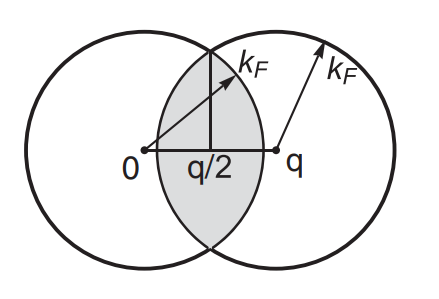
\includegraphics[scale=0.55]{figs/Jellium model/jellium_integration_region.png} }}
    \qquad
    \subfloat[\centering ]{{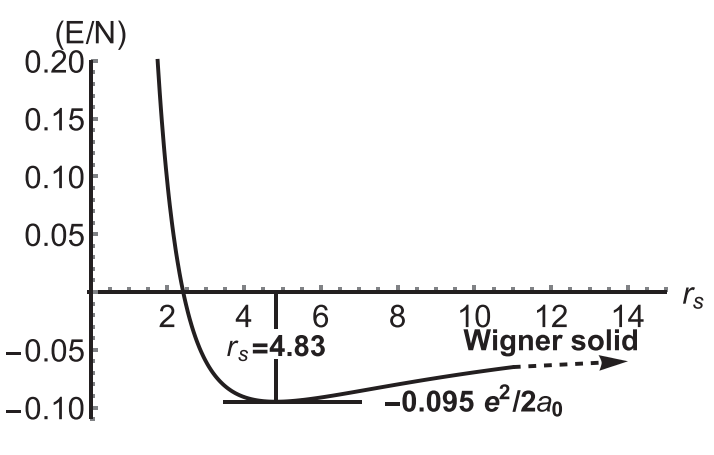
\includegraphics[scale=0.55]{figs/Jellium model/jellium_gse.png}}}
    \caption{Fig. A: Geometry for the ${\bf k}$-integration is shown for arbitrary, but fixed, ${\bf q}$, which is just the intersection of two spheres. \\
    Fig. B: Ground-state energy per electron, including first-order correction, for the jellium model.}
    \label{figs:jellium}
\end{figure}

\begin{equation}
    \begin{split}
        E^{(1)} &= \langle {\Omega} \bigg|  \sum_{\substack{{\bf k},{\bf k}',{\bf q} \in \Lambda\\
    \sigma \in \mathds{C}^2}} \frac{2\pi e^2}{\Omega q^2} {\bf c}_{{\bf k}+{\bf q} \blanky \sigma}^\dagger {\bf c}_{{\bf k}'-{\bf q} \blanky \sigma}^\dagger {\bf c}_{{\bf k}' \blanky \sigma} {\bf c}_{{\bf k} \blanky \sigma} \bigg| {\Omega} \rangle \\
    &= \langle {\Omega} \bigg|  \sum_{\substack{{\bf k},{\bf q} \in \Lambda\\
    \sigma \in \mathds{C}^2}} \frac{2\pi e^2}{\Omega q^2} {\bf c}_{{\bf k}+{\bf q} \blanky \sigma}^\dagger {\bf c}_{{\bf k} \sigma}^\dagger {\bf c}_{{\bf k}+{\bf q} \blanky \sigma} {\bf c}_{{\bf k} \sigma} \bigg| {\Omega} \rangle \\
    &= \langle {\Omega} \bigg|  \sum_{\substack{{\bf k},{\bf q} \in \Lambda\\
    \sigma \in \mathds{C}^2}} \frac{2\pi e^2}{\Omega q^2} (-N_{{\bf k}+{\bf q} \blanky \sigma} - N_{{\bf k} \sigma}) \bigg| {\Omega} \rangle  \Rightarrow \varepsilon^{(1)}({\bf k}) = - \frac{2\pi e^2}{\Omega} \sum_{{\bf q}} \frac{N_{{\bf k}} + {\bf q}}{q^2} \\
    \end{split}
\end{equation}
\begin{equation}
    \begin{split}
    \Rightarrow E^{(1)} &= -\frac{4\pi e^2}{\Omega} \frac{\Omega}{(2\pi)^6} \int_{\mathds{R}^6} d{\bf k} d{\bf q} \blanky \frac{1}{q^2} \Theta(k_F - |{\bf k} + {\bf q}|) \Theta(k_F - k) \textnormal{ with the integration region shown in \cref{figs:jellium} (left)}  \\
    &= - \frac{4\pi e^2 \Omega}{(2\pi)^6} \int_{\mathds{R}^3} \frac{d{\bf q}}{q^2} \int_{\mathds{R}^3} d{\bf p} \blanky \Theta\bigg(k_F - \bigg| {\bf p} + \frac{1}{2} {\bf q}\bigg|\bigg) \Theta\bigg(k_F - \frac{1}{2} {\bf q}\bigg) \\
    &= -\frac{e^2}{2a_0} N \frac{3}{2\pi} \bigg(\frac{9 \pi}{4}\bigg)^{\frac{1}{3}} \frac{1}{r_s}.
    \end{split}
\end{equation}

This results, shown in \cref{figs:jellium} (right), shows that the electron gas is stable when the repulsive Coulomb interaction is turned on. No external confinement potential is therefore needed to hold the electron gas in the ion jellium together. There exists an optimal density $n^*$, or interparticle distance $r_s^*$, which minimizes the energy and furthermore yields an $E^* < 0$. The negative exchange energy overcome the positive kinetic energy. This method of treating the electron gas is a special case of the Hartree-Fock approximation and is the simplest way to take into account interactions. The interesting point to note is that in this approximation the energy is reduced below that of the Sommerfeld gas, which is a manifestation of the exchange hole. 

\begin{figure}
    \centering
    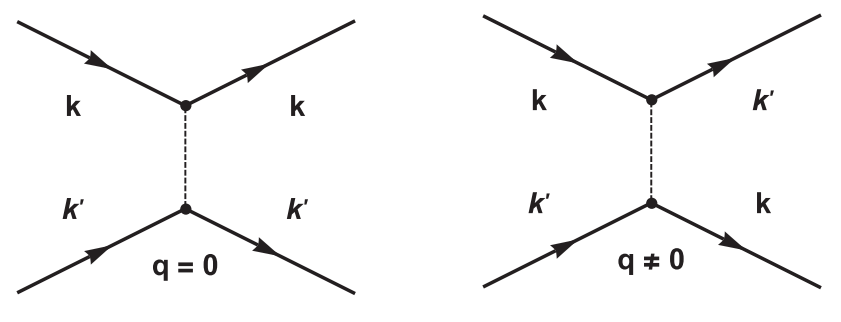
\includegraphics[scale  =.5]{figs/Jellium model/feynmann_diags.png}
    \caption{Diagrams for the jellium sea. The dashed line represents the interaction.}
    \label{fig:feynmann_jellium}
\end{figure}

\blanky \\

\paragraph{\textbf{Hartree-Fock approximation as a Mean-Field Theory}} \blanky \\

Consider the electronic Hamiltonian given by 
\cref{pre-HF-jellium H}. The goal is to write an effective two-body Hamiltonian, which takes into account the average effects of the interactions. Therefore, the four-Fermi interaction is replaced with a sum of all possible two-body terms

\begin{equation}
    \begin{split}
    \langle {\bf c}_1^\dagger {\bf c}_2^\dagger {\bf c}_3 {\bf c}_4 \rangle_{\textnormal{MFT}} &= - \langle {\bf c}_1^\dagger {\bf c}_3 \rangle {\bf c}_2^\dagger {\bf c}_4 -  \langle {\bf c}_2^\dagger {\bf c}_4 \rangle {\bf c}_1^\dagger {\bf c}_3 +  \langle {\bf c}_1^\dagger {\bf c}_4 \rangle {\bf c}_2^\dagger {\bf c}_3 +  \langle {\bf c}_2^\dagger {\bf c}_3 \rangle {\bf c}_1^\dagger {\bf c}_4, \\
    &\textnormal{ where } \langle {\bf c}_{{\bf k}\sigma}^\dagger {\bf c}_{{\bf k}'\sigma'} \rangle = {\bf n}_{{\bf k}\sigma} \delta_{{\bf k}{\bf k}'}^{\sigma \sigma'}
\end{split}\end{equation}

The mean field terms can be understood as the average number of particles ${\bf n}_{{\bf k}\sigma}$ in the $\ket{{{\bf k}\sigma}}$-state, which will be weighted with the two-body interaction $V({\bf q})$ to give the average interaction due to all other interaction terms. Then, the four-Fermi interaction in the mean-field approximation reads

\begin{equation}
\begin{split}
    \mathcal{V}_{\textnormal{HF}} = \frac{1}{2} \sum_{\substack{{\bf k}{\bf k}',{\bf q} \in \Lambda\\
    \sigma \sigma' \in \mathds{C}^2}} V({\bf q}) &\bigg[-\langle 
    {\bf c}_{{\bf k}\sigma}^\dagger {\bf c}_{{\bf k}'\sigma'}
    \rangle {\bf c}_{{\bf k}'-{\bf q} \blanky \sigma'}^\dagger {\bf c}_{{\bf k}-{\bf q} \sigma} 
    -  \langle {\bf c}_{{\bf k}'-{\bf q} \blanky \sigma'}^\dagger {\bf c}_{{\bf k}-{\bf q} \sigma}  \rangle {\bf c}_{{\bf k}\sigma}^\dagger {\bf c}_{{\bf k}'\sigma'} \\
    & \blanky \blanky \blanky + \langle {\bf c}_{{\bf k}\sigma}^\dagger {\bf c}_{{\bf k}-{\bf q} \sigma} \rangle {\bf c}_{{\bf k}'-{\bf q} \blanky \sigma'}^\dagger {\bf c}_{{\bf k}'\sigma'}
    +  \langle {\bf c}_{{\bf k}'-{\bf q} \blanky \sigma'}^\dagger {\bf c}_{{\bf k}'\sigma'} \rangle {\bf c}_{{\bf k}\sigma}^\dagger {\bf c}_{{\bf k}-{\bf q} \sigma} 
    \bigg] \\
    &= - \sum_{\substack{{\bf k}{\bf q} \in \Lambda\\
    \sigma \in \mathds{C}^2}} V({\bf q})  \langle {\bf c}_{{\bf k} \sigma}^\dagger {\bf c}_{{\bf k} \sigma} \rangle {\bf c}_{{\bf k}-{\bf q} \blanky \sigma}^\dagger {\bf c}_{{\bf k}-{\bf q} \blanky \sigma} + V(0) \sum_{\substack{{\bf k}{\bf k}' \in \Lambda\\
    \sigma \sigma' \in \mathds{C}^2}} \langle {\bf c}_{{\bf k} \sigma}^\dagger {\bf c}_{{\bf k} \sigma} \rangle  {\bf c}_{{\bf k}' \sigma'}^\dagger {\bf c}_{{\bf k}' \sigma'} \\
    &= \sum_{\substack{{\bf k} \in \Lambda\\
    \sigma \in \mathds{C}^2}} \bigg(-\sum_{{\bf q} \in \Lambda} {\bf n}_{{\bf k}+{\bf q} \sigma} V({\bf q}) + nV(0)\bigg){\bf c}_{{\bf k} \sigma}^\dagger {\bf c}_{{\bf k} \sigma}, \\
    \Rightarrow  {\bf H}^{\textnormal{HF}} &= \sum_{\substack{{\bf k} \in \Lambda\\
    \sigma \in \mathds{C}^2}} \varepsilon_{\bf k}^{\textnormal{HF}} {\bf c}_{{\bf k} \sigma}^\dagger {\bf c}_{{\bf k} \sigma}, \textnormal{ where } \begin{split}
        \varepsilon_{\bf k}^{\textnormal{HF}} &= \varepsilon_{\bf k} + \sum_{\substack{{\bf k}' \in \Lambda\\
    \sigma' \in \mathds{C}^2}} [V(0) - \delta_{\sigma\sigma'} V({\bf k}- {\bf k}')] {\bf n}_{{\bf k}' \sigma'} \\
        &= \varepsilon_{\bf k} + V(0) N - \sum_{\substack{{\bf k}' \in \Lambda\\
    \sigma' \in \mathds{C}^2}} V({\bf k}- {\bf k}') {\bf n}_{{\bf k'} \sigma'}.
    \end{split}
    \end{split}
\end{equation}

Note that the Hartree or direct Coulomb term, which represents the average interaction energy of the electron ${\bf k}\sigma$ with all the other electrons in the system, is a constant; when summed over all electron it cancels exactly with the constant arising from the sum of the self-energy of the positive background and the interaction energy of the electron gas with that of the background. The Fock, or exchange term, is a momentum-dependent shift. \\

\textbf{Problems with the Hartree-Fock Theory}

Although we argued that the Hartree-Fock approximation becomes a better approximation in the high-density limit for electron interacting via the Coulomb attraction, it never becomes exact. The Hartree-Fock energy correction is given by 

$$
    \varepsilon^{(1)}({\bf k}) = \frac{e^2 k_F}{4\pi^2} \bigg[\frac{k_F^2 - k^2}{kk_F} \log \bigg| \frac{k_F + k}{k_F - k}\bigg| + 2\bigg]
$$

The first term in parentheses has a logarithmic divergence in slope $k=kf$. This means that while the energy shift might be small compared to the Fermi energy, the Fermi velocity $v_F = \nabla_{{\bf k}} \varepsilon({\bf k})$, contains a non-finite term. This problem can be traced back to the long-range nature of the Coulomb force. Two electrons at large distances ${\bf x}-{\bf x}'$ do not feel the full $\frac{1}{|{\bf x}-{\bf x}'|}$-interaction, but a screened version due to the presence of the intervening medium, namely the electron gas, rearranges itself to cancel out the long-range part of $V$. \\

\underline{Electron Interaction in Second-order Perturbation Theory}

Trying to improve upon the first-order result by going to second-order perturbation theory yields a disastrous results for the matrix elements diverge. According to second-order perturbation theory, 

\begin{equation}
\frac{E^{(2)}}{N} = \frac{1}{N} \sum_{\substack{\ket{\psi} \in \mathds{H} \\
\ket{\psi} \neq \ket{\Omega}}} \frac{\bra{\Omega} {{\bf V}}_c \ket{\psi} \bra{\psi} {{\bf V}}_c \ket{\Omega}}{E^{(0)} - E_\psi}.
\end{equation}

\begin{figure}
    \centering
    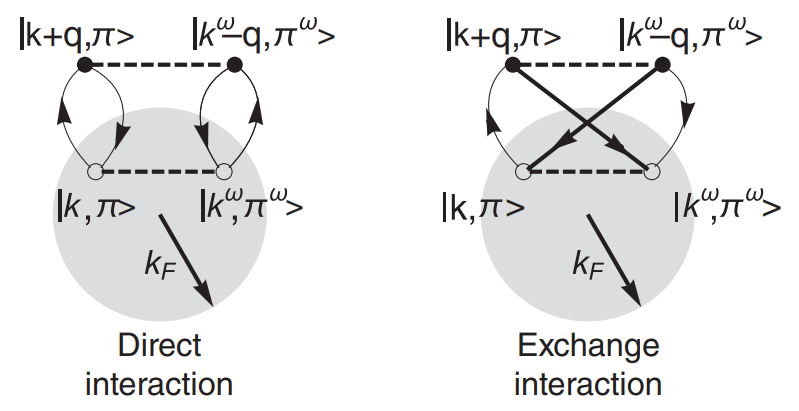
\includegraphics[scale = .5]{figs/Jellium model/fermi_sea_loops_second_order.png}
    \caption{The only two possible processes in second-order perturbation theory for two states, $\ket{{\bf k}_1, \sigma_1}$ and $\ket{{\bf k}_2, \sigma_2}$, in the Fermi sea. The direct process gives a divergent contribution to $\frac{E}{N}$ while the exchange process gives a finite contribution.}
    \label{fig:fermi_sea_loops_second_order}
\end{figure}

This, combined with the momentum-conserving Coulomb interaction, yields intermediate states where two particles are injected out of the Fermi sphere. From such an intermediate state, $\ket{\Omega}$, is restored by putting the excited electrons back into the holes they left behind. Therefore, the are only two types of possible processes: direct interaction and the exchange process, shown in \cref{fig:fermi_sea_loops_second_order}. \\

\begin{enumerate}
    \item In the \underline{Direct interaction}, it turns out that the direct interaction gives a divergent contribution $E^{(2)}_{\textnormal{dir}}$ to $E^{(2)}$ due to the singular behaviour of the Coulomb interaction at small ${\bf q}$-momentum transfers. The $(\ket{\psi} = \ket{\Omega})$-constraint leads to the second p
    
    $$
        \ket{\psi} = \Theta(|{\bf k}_1 + {\bf q}| - k_F) \Theta(|{\bf k}_2 - {\bf q}| - k_F) \Theta(k_F - |{\bf k}_2|) \Theta(k_F - |{\bf k}_1|) {\bf c}_{{\bf k}_1 + {\bf q}}^\dagger {\bf c}_{{\bf k}_2 - {\bf q}}^\dagger {\bf c}_{{\bf k}_2} {\bf c}_{{\bf k}_1} \ket{\Omega}.
    $$
    
    To restore $\ket{\Omega}$,  the same ${\bf q}$-momentum transfer must be involved in both $\bra{\Omega} {\bf V}_c \ket{\psi}$ and $\bra{\psi} {\bf V}_c \ket{\Omega}$, and writing ${\bf V}({\bf q}) = \frac{4 \pi e^2}{{\bf q}^2}$ yields
    
    \begin{equation}
    \begin{split}
    & E^{(2)}_{\textnormal{dir}} = \frac{1}{4 \Omega^2} \sum_{{\bf q} \in \Lambda} \sum_{\substack{{\bf k}{\bf k}' \in \Lambda\\
    \sigma \sigma' \in \mathds{C}^2}} \frac{{\bf V}({\bf q})^2}{E^{(0)} - E_{\nu}} \Theta(|{\bf k}_1 + {\bf q}| - k_F) \Theta(|{\bf k}_2 - {\bf q}| - k_F) \Theta(k_F - |{\bf k}_2|) \Theta(k_F - |{\bf k}_1|) \\
    & \textnormal{Given that ${\bf V}({\bf q})^2 \approx q^{-4}$} \Rightarrow E^{(0)} - E_{\psi} \overset{{\bf q} \rightarrow 0}{\approx} {\bf k}_1^2 + {\bf k}_2^2 - ({\bf k}_1+{\bf q})^2 - ({\bf k}_2 - {\bf q})^2 \approx q \\
    & \sum_{{\bf q} \in \Lambda} \sum_{\substack{{\bf k}{\bf k}' \in \Lambda\\
    \sigma \sigma' \in \mathds{C}^2}} \cdots \Theta(|{\bf k}_2 - {\bf q}| - k_F) \Theta(k_F - |{\bf k}_2|) \Theta(k_F - |{\bf k}_1|)  \overset{{\bf q} \rightarrow 0}{\approx} q \\
    & \Rightarrow E^{(2)}_{\textnormal{dir}} = \int_{0} dq q^2 \frac{1}{q^4} \frac{1}{q} q q = \int_{0} \frac{dq}{q} = \log q|_{0} \rightarrow \infty.
    \end{split}
    \end{equation}
    
    \blanky \\
    
    \item The exchange process does not lead to a divergence since, in this case, the momentum transfer in the excitation part is ${\bf q}$, but in the relaxation part it is ${\bf k}_2-{\bf k}_1-{\bf q}$. Thus ${\bf V}^2({\bf q})$ is replaced by ${\bf V}^2({\bf q}){\bf V}({\bf k}_2-{\bf k}_1-{\bf q}) \propto q^{-2}$ for ${\bf q} \rightarrow 0$, which is less singular than ${\bf V}^2({\bf q}) \propto q^{-4}$. \\  
\end{enumerate}

Physically, the energy of an electron gas must be finite. The only hope for rescue lies in regularization of the divergent behaviour by taking higher-order perturbation terms into account. Consider now the ground-state energy of the jellium model of a three-dimensional electron gas. In the $(r_s < 1)$-regime, this energy can be expressed in terms of a power-series in $r_s$, as

$$
    E_0 = \frac{K}{r_s^2} [1+ br_s + c r_s^2 + \cdots],
$$

where $K, a,b,c$ are constants. This is not exactly right, since first-order perturbation theory gives a term of the $(br_s)$-form in the series. But, considering second-order perturbation theory, one finds a contribution that diverges like $\int_0 \frac{dq}{q}$, where $q$ is the transfer-momentum in the Fourier transform ${\bf V}_q$ of the Coulomb interaction, ${\bf V}_q \approx q^{-2}$. Thus, there is in fact a logarithmic divergence from the lower limit $0$ of the momentum transfers. This divergence is associated with the long range of the Coulomb interaction. Furthermore, if one examines higher-order terms in the perturbation series, one finds that they diverge even more strongly. \\

On physical grounds, however, the energy of the interacting electron gas must be finite and well-defined, with no phase transitions occurring as the repulsive interactions are turned on. This failure of standard perturbation theory appears to signal that the energy does not have a standard power-series expansion in $r_s$. In 1957, Gell-Mann and Bruckner resolved this issue by developing many-body perturbation theory\footnote{Many-body perturbation expansions without diagrams.
I. Normal states. Behnam Farid §}, in which the summation of the divergent terms in the series an infinite number of terms) is performed before doing the momentum integrals, thus arriving to a finite and well-defined results. This is called the resummation of the perturbation series. They found that there was a term in the series for $E_0$ that is $\propto \log r_s$, and is non-analytic at $r_s = 0$. This holds so long the interaction doesn't cause any drastic changes to the system, such as a phase transition. \\

\subsection{Random Phase Approximation}

In the second quantization formalism, the fermionic field operators may be written in plane-wave basis as 

$$
    \Psi({\bf x}, t) = \frac{1}{\sqrt{\Omega}} \sum_{{\bf k} \in \Lambda} e^{i {\bf k} \cdot {\x}} {\bf c}_{{\bf k}}, \blanky \blanky \blanky \blanky 
    \Psi^\dagger({\bf x}, t) = \frac{1}{\sqrt{\Omega}} \sum_{{\bf k} \in \Lambda} e^{-i {\bf k} \cdot {\x}} {\bf c}_{{\bf k}}^\dagger.
$$

The particle density $\rho({\bf x})$ at point ${\bf x}$ is given by 

$$
    \rho({\bf x}) = \sum_{i \in \mathds{N}} \delta({\bf x} - {\bf x}_i) \Rightarrow \rho({\bf x}) = \int_{\mathds{R}^3} d{\bf x} \blanky \Psi^\dagger({\bf x}) \bigg(\sum_{i \in \mathds{N}} \delta({\bf x} - {\bf x}_i)\bigg) \Psi({\bf x}) = \sum_{i \in \mathds{N} }\Psi^\dagger({\bf x}) \Psi({\bf x}). 
$$

Its Fourier transform is given by ${\rho_{{\bf q}}} = \sum_{{\bf k} \in \Lambda} {\bf c}_{{\bf k}+{\bf q}}^\dagger {\bf c}_{\bf k}$. Its physical meaning is straightforward: it gives rise to particle-hole pairs charge fluctuations around the Fermi surface. Since $\rho^\dagger = \rho$, it follows that $\rho_{{\bf q}}^\dagger = \rho_{-{\bf q}}$. \footnote{For example, the following four-body term may be recast as 

$$
\sum_{{\bf k, k'} \in \Lambda} {\bf c}_{{\bf k}-{\bf q}}^\dagger {\bf c}_{{\bf k}'+{\bf q}}^\dagger {\bf c}_{{\bf k}'} {\bf c}_{{\bf k}} = - \sum_{{\bf k'} \in \Lambda} {\bf n}_{{\bf k}'} + \rho_{{\bf q}} \rho_{-{\bf q}'}.
$$}\\

Now, the following question naturally arises. Under what conditions an interacting system, with Hamiltonian 

$$
    {\bf H} = \sum_{{\bf k} \in \Lambda} \varepsilon_{{\bf k}} {\bf c}_{{\bf k}}^\dagger {\bf c}_{{\bf k}} + \frac{1}{2} \sum_{{\bf q} \in \Lambda} {\bf V}_{{\bf q}} (\rho_{{\bf q}} \rho_{-{\bf q}} - N),
$$

and ground-state $\ket{\Omega}$, ${\bf H} \ket{\Omega} = \varepsilon_0 \ket{\Omega}$, can support density excitations associated with $\rho_{{\bf q}}$? Namely, these excitations are

$$
    {\bf H} \rho_{{\bf q}}^\dagger \ket{\Omega} = (\varepsilon_0 + \hbar \omega_{{\bf q}}) \rho_{{\bf q}}^\dagger \ket{\Omega}
$$

\blanky \\

The previous equation may be rewritten as 

\begin{equation} 
\begin{split}
    [{\bf H}, \rho_{\bf q}^\dagger] = \hbar \omega_{{\bf q}} \rho_{{\bf q}}^\dagger  \Rightarrow & \bigg[\sum_{{\bf k} \in \Lambda} \varepsilon_{{\bf k}} {\bf c}_{{\bf k}}^\dagger {\bf c}_{{\bf k}} + \frac{1}{2} \sum_{{\bf q} \in \Lambda} {\bf V}_{{\bf q}} (\rho_{{\bf q}} \rho_{-{\bf q}} - N), \rho_{\bf q}^\dagger \bigg] = \hbar \omega_{{\bf q}} \rho_{{\bf q}}^\dagger \\
    & \bigg[\sum_{{\bf k} \in \Lambda} \varepsilon_{{\bf k}} {\bf c}_{{\bf k}}^\dagger {\bf c}_{{\bf k}}, \rho_{\bf q}^\dagger\bigg] + \frac{1}{2} \bigg[\sum_{{\bf q} \in \Lambda} {\bf V}_{{\bf q}} (\rho_{{\bf q}} \rho_{-{\bf q}} - N), \rho_{\bf q}^\dagger \bigg] = \\
    & \sum_{{\bf k} \in \Lambda} \varepsilon_{{\bf k}} \bigg[ {\bf c}_{{\bf k}}^\dagger {\bf c}_{{\bf k}}, \rho_{\bf q}^\dagger\bigg] + \frac{1}{2} \sum_{{\bf q} \in \Lambda} {\bf V}_{{\bf q}} \cancel{\bigg[\rho_{{\bf q}} \rho_{-{\bf q}}, \rho_{\bf q}^\dagger\bigg]} = \\
    & \sum_{{\bf k}, \mathfrak{k} \in \Lambda} \varepsilon_{{\bf k}} \bigg[ {\bf c}_{{\bf k}}^\dagger {\bf c}_{{\bf k}}, {\bf c}_{{\bf q}} {\bf c}_{{\bf \mathfrak{k} + q}}^\dagger \bigg] =  \\
    &\sum_{{\bf k}, \mathfrak{k} \in \Lambda} \varepsilon_{{\bf k}} \bigg({\bf c}_{{\bf k}}^\dagger \cancel{[{\bf c}_{{\bf k}}, {\bf c}_{{\bf q}}]} {\bf c}_{{\bf \mathfrak{k} + q}}^\dagger + [{\bf c}_{{\bf k}}^\dagger, {\bf c}_{{\bf q}}] {\bf c}_{{\bf k}} {\bf c}_{{\bf k}}^\dagger + {\bf c}_{{\bf q}} {\bf c}_{{\bf k}}^\dagger [{\bf c}_{{\bf k}}, {\bf c}_{{\bf \mathfrak{k} + q}}^\dagger] + {\bf c}_{{\bf q}} \cancel{[{\bf c}_{{\bf k}}^\dagger, {\bf c}_{{\bf \mathfrak{k} + q}}^\dagger]} {\bf c}_{{\bf k}} \bigg) = \\
    & \sum_{{\bf k} \in \Lambda} (\varepsilon_{{\bf k + q}} - \varepsilon_{{\bf k}}) {\bf c}_{{\bf {\bf k} + q}}^\dagger {\bf c}_{{\bf k}} = 
\end{split}
\end{equation}

If $\rho_{{\bf q}}^\dagger$ actually creates an excitation of energy $\hbar \omega$, then 

\begin{equation}
\begin{split}
    [{\bf H}, [{\bf H}, \rho_{\bf q}^\dagger]] = (\hbar \omega)^2 \rho_{{\bf q}}^\dagger \\
    \Rightarrow (\hbar \omega)^2 \rho_{{\bf q}}^\dagger &= \sum_{{\bf k} \in \Lambda} (\varepsilon_{{\bf k + q}} - \varepsilon_{{\bf k}}) [{\bf H}, {\bf c}_{{\bf {\bf k} + q}}^\dagger {\bf c}_{{\bf k}}] = \sum_{{\bf k} \in \Lambda} (\varepsilon_{{\bf k + q}} - \varepsilon_{{\bf k}})^2 {\bf c}_{{\bf k + q}}^\dagger {\bf c}_{{\bf k}} \\
    & \blanky \blanky \blanky \blanky+ \sum_{{\bf k}, {\bf q}' \in \Lambda} (\varepsilon_{{\bf k + q}} - \varepsilon_{{\bf k}}) \frac{V_{{\bf q}'}}{2} \bigg[({\bf c}_{{\bf {\bf k} + q - q'}}^\dagger {\bf c}_{{\bf k}} - {\bf c}_{{\bf k + q}}^\dagger {\bf c}_{{\bf {\bf k} + q'}}) \rho_{{\bf q}'}^\dagger + \rho_{{\bf q}'} ({\bf c}_{{\bf {\bf k} + q + q'}}^\dagger {\bf c}_{{\bf k}} - {\bf c}_{{\bf k + q}}^\dagger {\bf c}_{{\bf {\bf k} - q'}})\bigg] \\
    &= \sum_{{\bf k} \in \Lambda} \bigg[ \frac{\hbar^2}{2m} (2 {\bf k} \cdot {\bf q} + {\bf q}^2)\bigg]^2 {\bf c}_{{\bf k}+{\bf q}}^\dagger {\bf c}_{{\bf k}} + \sum_{{\bf k}, {\bf q}' \in \Lambda} \frac{V_{\bf q'}}{2}\bigg[\frac{\hbar^2}{2m}(2 {\bf k}\cdot {\bf q} + {\bf q}^2) ({\bf c}_{{\bf {\bf k} + q - q'}}^\dagger {\bf c}_{{\bf k}} - {\bf c}_{{\bf k + q}}^\dagger {\bf c}_{{\bf {\bf k} + q'}}) \\ & \blanky \blanky \blanky \blanky - \frac{\hbar^2}{2m}(2 {\bf k}\cdot {\bf q} + {\bf q}^2) ({\bf c}_{{\bf {\bf k} + q + q'}}^\dagger {\bf c}_{{\bf k}} - {\bf c}_{{\bf k + q}}^\dagger {\bf c}_{{\bf {\bf k} - q'}})\bigg] \\
    &= \sum_{{\bf k} \in \Lambda} \bigg[ \frac{\hbar^2}{2m} (2 {\bf k} \cdot {\bf q} + {\bf q}^2)\bigg]^2 {\bf c}_{{\bf k}+{\bf q}}^\dagger {\bf c}_{{\bf k}} + \sum_{{\bf q}' \in \Lambda} \frac{V_{\bf q'}}{2} \bigg[ \sum_{{\bf k} \in \Lambda}\frac{\hbar^2}{2m}(2 {\bf k}\cdot {\bf q} + {\bf q}^2) ({\bf c}_{{\bf {\bf k} + q - q'}}^\dagger {\bf c}_{{\bf k}} - {\bf c}_{{\bf k + q}}^\dagger {\bf c}_{{\bf {\bf k} + q'}}) \\ 
    & \blanky \blanky \blanky \blanky - \sum_{{\bf k} \in \Lambda}\frac{\hbar^2}{2m}(2 {\bf k}\cdot {\bf q} + {\bf q}^2) ({\bf c}_{{\bf {\bf k} + q + q'}}^\dagger {\bf c}_{{\bf k}} - {\bf c}_{{\bf k + q}}^\dagger {\bf c}_{{\bf {\bf k} -
    q'}})\bigg] \\
    &= \sum_{{\bf k} \in \Lambda} \bigg[ \frac{\hbar^2}{2m} (2 {\bf k} \cdot {\bf q} + {\bf q}^2)\bigg]^2 {\bf c}_{{\bf k}+{\bf q}}^\dagger {\bf c}_{{\bf k}} \\
    & + \sum_{{\bf q}' \in \Lambda} \frac{V_{\bf q'}}{2} \bigg[ \sum_{{\bf k} \in \Lambda}\frac{\hbar^2}{2m}(2 {\bf k}\cdot {\bf q} + {\bf q}^2) {\bf c}_{{\bf {\bf k} + q - q'}}^\dagger {\bf c}_{{\bf k}} - \frac{\hbar^2}{2m}(2 {\bf k}\cdot {\bf q} + {\bf q}^2) {\bf c}_{{\bf k + q}}^\dagger {\bf c}_{{\bf {\bf k} + q'}} \\
    & \blanky \blanky \blanky \blanky - \sum_{{\bf k} \in \Lambda}\frac{\hbar^2}{2m}(2 {\bf k}\cdot {\bf q} + {\bf q}^2) {\bf c}_{{\bf {\bf k} + q + q'}}^\dagger {\bf c}_{{\bf k}} - \frac{\hbar^2}{2m}(2 {\bf k}\cdot {\bf q} + {\bf q}^2) {\bf c}_{{\bf k + q}}^\dagger {\bf c}_{{\bf {\bf k} - q'}}\bigg] \\
    \end{split}
\end{equation}

\begin{equation}
    \begin{split}
 \blanky  
&= \sum_{{\bf k} \in \Lambda} \bigg[ \frac{\hbar^2}{2m} (2 {\bf k} \cdot {\bf q} + {\bf q}^2)\bigg]^2 {\bf c}_{{\bf k}+{\bf q}}^\dagger {\bf c}_{{\bf k}} \blanky \blanky \blanky \blanky \blanky \blanky \textnormal{  let ${\bf k}' = {\bf k} + {\bf q}'$, ${\bf k}'' = {\bf k} - {\bf q}'$}\\
 & \blanky \blanky \blanky \blanky + \sum_{{\bf q}' \in \Lambda} \frac{V_{\bf q'}}{2} \bigg[ \sum_{{\bf k} \in \Lambda}\frac{\hbar^2}{2m}(2 {\bf k}\cdot {\bf q} + {\bf q}^2) {\bf c}_{{\bf {\bf k} + q - q'}}^\dagger {\bf c}_{{\bf k}} - \sum_{{\bf k}' \in \Lambda}\frac{\hbar^2}{2m}(2 ({\bf k}' - {\bf q}')\cdot {\bf q} + {\bf q}^2) {\bf c}_{{\bf k' + q - q'}}^\dagger {\bf c}_{{\bf {\bf k}'}}\\ 
 & \blanky \blanky \blanky \blanky - \sum_{{\bf k} \in \Lambda}\frac{\hbar^2}{2m}(2 {\bf k}\cdot {\bf q} + {\bf q}^2) {\bf c}_{{\bf {\bf k} + q + q'}}^\dagger {\bf c}_{{\bf k}} - \sum_{{\bf k}'' \in \Lambda}\frac{\hbar^2}{2m}(2 ({\bf k}'' + {\bf q}')\cdot {\bf q} + {\bf q}^2) {\bf c}_{{\bf k'' + q + q'}}^\dagger {\bf c}_{{\bf {\bf k}''}} \bigg] \\
    \end{split}
\end{equation}

\begin{align}
     \alignedbox{(\hbar \omega)^2 \rho_{{\bf q}}^\dagger}{= \sum_{{\bf k} \in \Lambda} \bigg[ \frac{\hbar^2}{2m} (2 {\bf k} \cdot {\bf q} + {\bf q}^2)\bigg]^2 {\bf c}_{{\bf k}+{\bf q}}^\dagger {\bf c}_{{\bf k}} + \sum_{{\bf q}' \in \Lambda} \frac{V_{\bf q'}}{2} \frac{\hbar^2 {\bf q} \cdot {\bf q}'}{m} \bigg(\rho_{{\bf q}' - {\bf q}} \rho_{{\bf q}'}^\dagger - \rho_{{-{\bf q}'}}^\dagger \rho_{-{\bf q} - {\bf q}'} \bigg).}
     \label{RPA-basis equation}
\end{align}

\begin{figure}
    \centering
    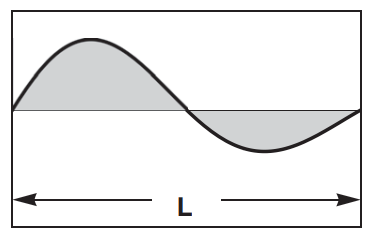
\includegraphics[scale = .5]{figs/Jellium model/RPA-fig.png} 
    \caption{Consider a length-$L$ box. Then, $\rho_q$ measures the quantity approximately equal to the difference in the particle number in the two halves of the container. }
    \label{fig:RPA-box}
\end{figure}

Now, in order to study \cref{RPA-basis equation}, note that $\rho_0$ is actually much larger than all the other components. It is just the average particle density in the system. Consider a box of length-$L$, shown in \cref{fig:RPA-box}, containing a large number of electrons of $\rho_0$ average density, then $\rho_0$'s first Fourier component is 

$$
    \int_{\Omega \subset \R^3} d{\bf x} \blanky \rho({\bf x}) e^{\frac{2i \pi x}{L}},
$$

will be approximately equal to the difference between the particle number in the left and right hand sides of the box, the gray area. The number difference will then be small, compared to the total number and so $\rho_0$ will prevail in the summation over ${\bf q}'$. Since the $({\bf q}' = 0)$-term is omitted, $\rho_0$ will only appear when ${\bf q}' = \pm {\bf q}$. The neglect of all other terms, when ${\bf q}' \neq \pm {\bf q}$ is known as the \textbf{random phase approximation} \footnote{An alternative interpretation for the RPA is as follows. Consider the first-quantized version of the density operator $\rho_{{\bf q} \in \Lambda} = \frac{1}{\Omega} \sum_{n \in \mathds{N}} e^{i {\bf q} \cdot {\bf x}_n}$, where ${\bf x}_n$ is the $n$-th's particles position. Then, $\rho_{{\bf q} \pm {\bf q}'}$ may be written in first quantized form as 

$$
    \rho_{{\bf q} \pm {\bf q}'} \frac{1}{\Omega} \sum_{n \in \mathds{N}} e^{i ({\bf q} \pm {\bf q}') \cdot {\bf x}_n}.
$$

Then, if the electrons are statistically randomly distributed in the system, the preceding sum only gives a finite result if ${\bf q} = \mp {\bf q'}$, since the sum involves random phases that add destructively. In RPA, \cref{RPA-basis equation} is approximated by keeping only terms with ${\bf q} = \mp {\bf q}'$. }.\\

\underline{Plasma oscillations}

Consider the case where ${\bf q}$ is small enough that, for the moment, the first term in \cref{RPA-basis equation} may be neglected and the second term approximated via RPA. In that case, 

$$
(\hbar \omega)^2 \rho_{{\bf q}}^\dagger = \frac{4\pi e^2}{q^2} \frac{\hbar^2 q^2}{m} (\rho_0 \rho_{{\bf q}}^\dagger + \rho_{{\bf q}}^\dagger \rho_0 ) \rightarrow \omega^2 = \frac{4\pi e^2 \rho_0}{m},
$$

which gives just the classical plasma frequency $\omega_P$. The contribution of the first term may be approximated by setting $k \sim k_F$ and $\langle 2 {\bf k}_F \cdot {\bf q} \rangle >> {\bf q}^2$. Averaging over all angles yields

$$
\langre ({\bf k}_F \cdot {\bf q})^2 \rangle \simeq \frac{1}{4\pi} 4\pi^2 k_F^2 q^2 \int_{-1}^{1} dx x^2 = 2\pi k_F^2 q^2, 
$$

which yield the plasmon dispersion relation

$$
\omega^2({\bf q}) = \omega_P^2 + \frac{2\pi \hbar^2 k_F^2}{3m^2} q^2 \simeq \omega_P + \frac{\pi v_F^2}{3\omega_P} q^2. 
$$

Thus, the relevant long-wavelength excitations are collective motions of the electron gas. Bohm and Pines suggested that electrons act as interacting particles through a bare Coulomb potential $\frac{4\pi e^2}{q^2}$ only for length scales less than an effective screening length, which may be taken to be the Thomas-Fermi distance, $\sim q_{\textnormal{TF}}^{-1}$. Below $q_{\textnormal{TF}}$, the interaction contribute only to the plasma oscillations. \\

\subsection{Green Functions for Many-Body systems.}

Green function techniques play a fundamental role in the treatment of many-body systems, for many properties of a many body system -eg. ground state energy, excitation spectra, response functions, electric and magnetic susceptibilities and thermodynamic quantities- can be derived from many-body Green functions.\\

Consider the ground state $\ket{\Omega}$ of a system. At some time $t'$, a perturbation is enacted upon the system, said perturbation represented by a local operator ${\bf O}^\dagger({\bf x}, t)$, creating an initial state ${\bf O}^\dagger({\bf x}', t') \ket{\Omega}$. Thus, the system has been deviated from the initial some by some local excitations, a disturbance, and then this disturbance will evolve in space and time. Such a scenario describes typical local measurements done on a quantum many-particle system. Since an explicit time dependence is necessary for this formalism, the Heisenberg picture is useful. To determine physically interesting quantities, the quantum-mechanical amplitude to find the system in state ${\bf O}^\dagger({\bf x}', t') \ket{\Omega}$ at time $t > t'$ namely, 

$$
    \mathcal{A} = \bra{\Omega} {{\bf O}}({{\bf x}}, t) {{\bf O}}^\dagger({{\bf x}}', t') \ket{\Omega}.
$$

Many quantum-mechanical operators may be written in bilinear forms of the field operators themselves, $\hat{\Psi}({{\bf x}}, t)$. However, it turns out that correlation functions of the field operators are related to experiments such as photoemission and tunnelling spectroscopies, which involve extraction or injection of a single electron. These field correlation functions can be identified as propagators which satisfy the Green function equation. \\

\subsubsection{The One-Particle Green Function of Many-Body Systems}

\paragraph{Non-interacting Particle Propagator}

Consider a particle in free space described by a single-particle time-independent Hamiltonian ${\bf H}_1$. Its eigenstates and eigenenergies are 

$$
    {\bf H}_1 \ket{\phi_n} = \varepsilon_n \ket{\phi_n}.
$$

In general, if a particle is in the $\ket{\phi}_i$-state, it will remain in that state forever. Instead, consider a system in a generic state $\ket{\psi_{\textnormal{trial}}}$. If the trial state is created at time $t'$, the wave-function at a later time $t$ is given by 

$$
    \ket{\psi(t)} = e^{-\frac{i {\bf H} (t-t')}{\hbar}} \ket{\psi_{\textnormal{trial}}} = \sum_{n} \ket{\psi_n} e^{-\frac{i \varepsilon_n (t-t')}{\hbar}} \bar{\phi_n}\ket{\psi_{\textnormal{trial}}}.
$$

Then, at time $t$, the probability amplitude that a measurement would find the particle at position ${\bf x}$ can be found as

\begin{equation}
    \begin{split}
        \bra{{\bf x}} \ket{\psi(t)} \Theta(t-t') &= \int_{\R^3} d{\bf x}' \blanky \bra{{\bf x}} e^{-\frac{i {\bf H} (t-t')}{\hbar}} \ket{{\bf x}'}\bra{{\bf x}'} \ket{\psi_{\textnormal{trial}}} \Theta(t-t') \\
        &=  \int_{\R^3} d{\bf x}' \sum_{n \in \mathds{N}} \blanky \bra{{\bf x}} \ket{\phi_n} e^{-\frac{i \varepsilon_n (t-t')}{\hbar}} \bra{\phi_n}\ket{{\bf x}'}\bra{{\bf x}'} \ket{\psi_{\textnormal{trial}}} \Theta(t-t') \\
        &= i \int_{\R^3} d{\bf x}' \blanky \mathfrak{G}^{\textnormal{R}}({\bf x}t, {\bf x}'t') \psi_{\textnormal{trial}}({\bf x}', t'), \begin{array}{c}
             \textnormal{ where } \mathfrak{G}^{\textnormal{R}}({\bf x}t, {\bf x}'t') = - i \Theta(t-t') \bra{{\bf x}} e^{-\frac{i {\bf H} (t-t')}{\hbar}} \ket{{\bf x}'} \\
             \textnormal{ is the retarded Green function, or propagator,} \\
             \textnormal{ in coordinate representation.}
        \end{array}
    \end{split} 
    \label{NR-1particle-GF}
\end{equation}

Note that the time translational invariance is apparent due to the Hamiltonian's dependence on $\tau = t-t'$. Therefore, if the Green function $\mathfrak{G}^{\textnormal{R}}({\bf x}t, {\bf x}'t')$ is known, then it can be used to calculate the evolution of any initial state. Interesting information can be extracted from the propagator. 

\begin{itemize}
    \item The bracket $\bra{\phi_n}\ket{{\bf x}} = \bra{\phi_n} \psi_n^\dagger({\bf x}) \ket{0}$ is just the probability amplitude of forcing the system to collapse into the eigenstate $\ket{\psi_n}$ when a particle is inserted at position ${\bf x}$ and its energy is measured immediately afterwards. \\
    \item Its resolvant can also be found. From \cref{NR-1particle-GF}, note that the time evolution is a superposition of waves propagating with different energies. In principle, it could be used to determine the eigenspectrum. This can be done via a Fourier transform to the frequency domain\footnote{Note that the Fourier transform is ill-defined, given the oscillatory behaviour for $t \rightarrow \infty$. Therefore, according to the Sokhotoski-Plemelj formula, the new function
        $$
            e^{-\eta |t| }\mathfrak{G}^{\textnormal{R}}({\bf x}, {\bf x}'; \omega), \textnormal{ with } \eta > 0,
        $$
        is considered.},
    
    \begin{equation}
    \begin{split}
        \mathfrak{G}^{\textnormal{R}}({\bf x}, {\bf x}'; \omega) &= \mathcal{F}[        \mathfrak{G}^{\textnormal{R}}({\bf x}t, {\bf x}'t')]({\bf x}, {\bf x}'; \omega) \\
        &= \int dt \blanky e^{i(\omega + i \eta) \tau} \bra{{\bf x}} e^{-\frac{i {\bf H} \tau}{\hbar}} \ket{{\bf x}'} = \bigg\langle {\bf x} \bigg| \frac{1}{\omega - {\bf H} + i \eta} \bigg| {{\bf x}'}\bigg\rangle,
    \end{split}
    \end{equation}
    
    where the Sokhotoski-Plemelj formula has been used. This is just the resolvent whose poles constitute the quantum system's spectrum. \\
    
    Operationally, we can dvise a gedankenexperiment in which the particle is initially inserted at ${\bf x}'$-position and picked up at ${\bf x}$-position after some time $t$. When performing this recipe with adequate resolution and for a sufficiently large number of different positions and elapsed times, the Fourier transform of the record data would provide the full eigenvalue spectrum. Such an experiment would give complete information on our particle. 
\end{itemize}

This scenario thus reveals that all observables can be expressed in terms of the Green function and thus avoid the explicit use of the wavefunctions. \\

\underline{Differential Equation for the Green Function} \\

Consider \cref{NR-1particle-GF}. The LHS's time derivative will yield

\begin{equation}
    \begin{split}
        &\bra{{\bf x}} \ket{\psi(t)} \Theta(t-t') = i \int_{\R^3} d{\bf x}' \blanky \mathfrak{G}^{\textnormal{R}}({\bf x}t, {\bf x}'t') \psi_{\textnormal{trial}}({\bf x}', t') \\
        &i \delta(t-t') \psi({\bf x}, t) + i \Theta(t-t') \frac{\partial \psi({\bf x}, t)}{\partial t} = i \frac{\partial}{\partial t} \bigg(i \int_{\R^3} d{\bf x}' \blanky \mathfrak{G}^{\textnormal{R}}({\bf x}t, {\bf x}'t') \psi({\bf x}', t') \bigg) \\
        & i \delta(t-t') \int_{\R^3} d{\bf x}' \blanky \delta({\bf x}- {\bf x}') \psi({\bf x}, t) + {\bf H} \Theta(t-t') ({\bf x}) \frac{\partial \psi({\bf x}, t)}{\partial t} = i \frac{\partial}{\partial t} \bigg(i \int_{\R^3} d{\bf x}' \blanky \mathfrak{G}^{\textnormal{R}}({\bf x}t, {\bf x}'t') \psi({\bf x}', t') \bigg) \\
        & i \delta(t-t') \int_{\R^3} d{\bf x}' \blanky \delta({\bf x}- {\bf x}') \psi({\bf x}, t) + {\bf H} \bigg(i \int_{\R^3} d{\bf x}' \blanky \mathfrak{G}^{\textnormal{R}}({\bf x}t, {\bf x}'t') \psi_{\textnormal{trial}}({\bf x}', t')\bigg) = i \frac{\partial}{\partial t} \bigg(i \int_{\R^3} d{\bf x}' \blanky \mathfrak{G}^{\textnormal{R}}({\bf x}t, {\bf x}'t') \psi({\bf x}', t') \bigg) \\
        &\int_{\R^3} d{\bf x}' \blanky \bigg(i \frac{\partial}{\partial t} - {\bf H}\bigg) \mathfrak{G}^{\textnormal{R}}({\bf x}t, {\bf x}'t') \psi({\bf x}', t') = i \delta(t-t') \int_{\R^3} d{\bf x}' \blanky \delta({\bf x}- {\bf x}') \psi({\bf x}, t) \\
        & \Rightarrow  \bigg(i \frac{\partial}{\partial t} - {\bf H}\bigg) \mathfrak{G}^{\textnormal{R}}({\bf x}t, {\bf x}'t') = \delta(t-t') \delta({\bf x}- {\bf x}'),
    \end{split}
\end{equation}

which is just the definition of the Green function for the Schr\"odinger equation in differential equation form
\iffalse\footnote{Another, equivalent deriviation is as follows,

\begin{equation}
    \begin{split}
        &\bra{{\bf x}} \ket{\psi(t)} \Theta(t-t') = i \int_{\R^3} d{\bf x}' \blanky \mathfrak{G}^{\textnormal{R}}({\bf x}t, {\bf x}'t') \psi_{\textnormal{trial}}({\bf x}', t') \\
        &i \delta(t-t') \psi({\bf x}, t) + i \Theta(t-t') \frac{\partial \psi({\bf x}, t)}{\partial t} = i \frac{\partial}{\partial t} \bigg(i \int_{\R^3} d{\bf x}' \blanky \mathfrak{G}^{\textnormal{R}}({\bf x}t, {\bf x}'t') \psi({\bf x}', t') \bigg) \\
        & i \delta(t-t') \psi({\bf x}, t) + \Theta(t-t') {\bf H}({\bf x}) \frac{\partial \psi({\bf x}, t)}{\partial t} = i \int_{\R^3} d{\bf x}' \blanky \frac{\partial}{\partial t} \bigg( - i \Theta(t-t') \bra{{\bf x}} e^{-\frac{i {\bf H} (t-t')}{\hbar}} \ket{{\bf x}'}\bigg) \psi({\bf x}', t') \\
        &  i \delta(t-t') \psi({\bf x}, t) + \Theta(t-t') {\bf H}({\bf x}) \frac{\partial \psi({\bf x}, t)}{\partial t} = i \int_{\R^3} d{\bf x}' \blanky \bigg(\frac{\partial}{\partial t} \Theta(t-t')\bigg) \bra{{\bf x}} e^{-\frac{i {\bf H} (t-t')}{\hbar}} \ket{{\bf x}'} \psi({\bf x}', t') \\
        & \blanky\blanky\blanky\blanky\blanky\blanky\blanky\blanky\blanky\blanky\blanky\blanky\blanky\blanky\blanky\blanky\blanky\blanky\blanky\blanky\blanky\blanky\blanky\blanky\blanky\blanky\blanky\blanky\blanky\blanky\blanky\blanky \blanky\blanky\blanky\blanky\blanky\blanky\blanky\blanky\blanky\blanky\blanky\blanky\blanky\blanky\blanky\blanky\blanky\blanky\blanky\blanky\blanky\blanky\blanky\blanky\blanky\blanky\blanky\blanky\blanky\blanky\blanky\blanky\blanky\blanky\blanky\blanky\blanky\blanky\blanky\blanky\blanky\blanky\blanky\blanky\blanky + i \int_{\R^3} d{\bf x}' \blanky \Theta(t-t') \bigg(\frac{\partial}{\partial t} \bra{{\bf x}} e^{-\frac{i {\bf H} (t-t')}{\hbar}} \ket{{\bf x}'} \bigg) \psi({\bf x}', t')\\
        &  i \delta(t-t') \psi({\bf x}, t) + \Theta(t-t') {\bf H}({\bf x}) \frac{\partial \psi({\bf x}, t)}{\partial t} = i \int_{\R^3} d{\bf x}' \blanky \delta(t-t') \bra{{\bf x}} e^{-\frac{i {\bf H} (t-t')}{\hbar}} \ket{{\bf x}'} \psi({\bf x}', t') \\
        & \blanky\blanky\blanky\blanky\blanky\blanky\blanky\blanky\blanky\blanky\blanky\blanky\blanky\blanky\blanky\blanky\blanky\blanky\blanky\blanky\blanky\blanky\blanky\blanky\blanky\blanky\blanky\blanky\blanky\blanky\blanky\blanky \blanky\blanky\blanky\blanky\blanky\blanky\blanky\blanky\blanky\blanky\blanky\blanky\blanky\blanky\blanky\blanky\blanky\blanky\blanky\blanky\blanky\blanky\blanky\blanky\blanky\blanky\blanky\blanky\blanky\blanky\blanky\blanky\blanky\blanky\blanky\blanky\blanky\blanky\blanky\blanky\blanky\blanky\blanky\blanky\blanky + i {\bf H}({\bf x}) \int_{\R^3} d{\bf x}' \blanky \Theta(t-t') \mathfrak{G}^{\textnormal{R}}({\bf x}t, {\bf x}'t') \psi({\bf x}', t')\\
        &  i \delta(t-t') \psi({\bf x}, t) + {\bf H}({\bf x}) \frac{\partial \psi({\bf x}, t)}{\partial t} = i \delta(t-t') \int_{\R^3} d{\bf x}' \blanky \delta({\bf x}- {\bf x}')\psi({\bf x}', t') \\
        & \blanky\blanky\blanky\blanky\blanky\blanky\blanky\blanky\blanky\blanky\blanky\blanky\blanky\blanky\blanky\blanky\blanky\blanky\blanky\blanky\blanky\blanky\blanky\blanky\blanky\blanky\blanky\blanky\blanky\blanky\blanky\blanky \blanky\blanky\blanky\blanky\blanky\blanky\blanky\blanky\blanky\blanky\blanky\blanky\blanky\blanky\blanky\blanky\blanky\blanky\blanky\blanky\blanky\blanky\blanky\blanky\blanky\blanky\blanky\blanky\blanky\blanky\blanky\blanky\blanky\blanky\blanky\blanky\blanky\blanky\blanky\blanky\blanky\blanky\blanky\blanky\blanky + i {\bf H}({\bf x}) \int_{\R^3} d{\bf x}' \blanky  \mathfrak{G}^{\textnormal{R}}({\bf x}t, {\bf x}'t') \psi({\bf x}', t')
    \end{split}
\end{equation}
}\fi

\subsubsection{One-particle Green Function of Many-Body Systems}

The notion of a Green function can be applied to situations in which a particle is injected into a system containing many similar interacting particles and subsequently remove it from the system. Conversely, a particle can be removed from the system and then inject it back. This process may induce non-trivial collective excitations on the system. Physically, an interesting quantity would be the correlation function. \\

Consider a zero-temperature sstem. The one-particle Green function is defined, in the position representation, as 

\begin{equation}
    i \mathfrak{G}_{\alpha \beta} ({\bf x}t, {\bf x}'t') = \frac{\bra{\Omega} \mathcal{T} [\hat{\psi}_{H \alpha}({\bf x}, t) \hat{\psi}^\dagger_{H \beta}({\bf x}', t')] \ket{\Omega}}{\bra{\Omega}\ket{\Omega}},
    \label{SR-1particle-GF}
\end{equation}

where \begin{itemize}
    \item $\ket{\Omega}$ is the ground state of the interacting system in the Heisenberg picture,
    \item and $\hat{\psi}_{H \alpha}({\bf x}, t)$ is a Heisenberg field operator, which can be written in terms of the corresponding Schr\"odinger field operator as $\hat{\psi}_{H \alpha}({\bf x}, t) = e^{\frac{i {\bf H} t}{\hbar}} \hat{\psi}_{H \alpha}({\bf x}, t) e^{-\frac{i {\bf H} t}{\hbar}}$, 
    \item and where $\alpha$ represents a set of quantum numbers associated with the particle, eg. spin, momentum etc. \item $\mathcal{T}$ is the time-ordering operator, whose definition is as follows 
    
    \begin{equation} \begin{split}
        \mathcal{T} [\hat{\psi}_{H \alpha}({\bf x}, t) \hat{\psi}_{H \beta}({\bf x}', t')] &= \left\{ \begin{array}{cc}
           \hat{\psi}_{H \alpha}({\bf x}, t) \hat{\psi}^\dagger_{H \beta}({\bf x}', t') & t > t' \\ 
           -  \hat{\psi}^\dagger_{H \beta}({\bf x}', t')   \hat{\psi}_{H \alpha}({\bf x}, t) & t' > t 
        \end{array}\right. \\
        &= \Theta(t-t')\hat{\psi}_{H \alpha}({\bf x}, t) \hat{\psi}^\dagger_{H \beta}({\bf x}', t') - \Theta(t'-t)\hat{\psi}^\dagger_{H \beta}({\bf x}', t')   \hat{\psi}_{H \alpha}({\bf x}, t),
    \end{split}
    \end{equation}
    
    where the minus sign arises from the anticommutation of the fermionic field operators. \\
\end{itemize}

Now, \cref{SR-1particle-GF}'s one-particle nature is due to the fact that it represents a propagator of a particle created at ${\bf x}', t'$ with quantum numbers $\beta$, and annihilated at ${\bf x}, t$ with quantum numbers $\alpha$. Note, however, that these so-called single-particle Green functions are truly many-body objects since they describe the propagation of a single particle obeying the full many-body Hamiltonian and therefore contain all effects of interactions with the other particles in the system. \\

Depending on the problem at hand, there are a number of useful Green functions. The greater and lesser Green functions are defined as 

\begin{equation}
    \begin{split}
       \mathfrak{G}^{>}({\bf x}t, {\bf x}' t') = -i \bra{\Omega}\hat{\psi}_{H \alpha}({\bf x}, t) \hat{\psi}^\dagger_{H \beta}({\bf x}', t') \ket{\Omega}
        \\
       \mathfrak{G}^{<}({\bf x}t, {\bf x}' t') = \pm i \bra{\Omega} \hat{\psi}^\dagger_{H \beta}({\bf x}', t') \hat{\psi}_{H \alpha}({\bf x}, t) \ket{\Omega}
    \end{split}, \begin{array}{c}
         \textnormal{ where the + and - signs are for}  \\
         \textnormal{ fermions and bosons, respectively. }
    \end{array}
\end{equation}

The retarded and advanced Green functions are 

\begin{equation}
    \begin{split}
         \mathfrak{G}^{\textnormal{R}}({\bf x}t, {\bf x}' t') = \left\{\begin{array}{c}
              -i \Theta(t-t')  \bra{\Omega}[\hat{\psi}_{H \alpha}({\bf x}, t),  \hat{\psi}^\dagger_{H \beta}({\bf x}', t')]_{\pm} \ket{\Omega}   \\
              \Theta(t-t') \bigg[\mathfrak{G}^{>}({\bf x}t, {\bf x}' t') - \mathfrak{G}^{<}({\bf x}t, {\bf x}' t')\bigg]
         \end{array} \right. \\
         \mathfrak{G}^{\textnormal{A}}({\bf x}t, {\bf x}' t') = \left\{\begin{array}{c}
              i \Theta(t-t')  \bra{\Omega}[\hat{\psi}^\dagger_{H \beta}({\bf x}', t'), \hat{\psi}_{H \alpha}({\bf x}, t)]_{\pm} \ket{\Omega}   \\
              \Theta(t-t') \bigg[\mathfrak{G}^{<}({\bf x}t, {\bf x}' t') - \mathfrak{G}^{>}({\bf x}t, {\bf x}' t')\bigg]
         \end{array} \right. 
 \end{split}
\end{equation}

For compactness, $\bra{\Omega} \ket{\Omega} = 1$. Note that, from these definitions, $ \mathfrak{G}^{\textnormal{R}} = 0$, for $t < t'$ and $ \mathfrak{G}^{\textnormal{A}} = 0$, for $t > t'$. So far these Green functions are the space-time Green functions, since they involve creation and annihilation of particles at definite locations in space and time. Analogous Green functions may be defined in other basis. For example, in translationally invariant systems in space-time, the momentum-frequency domain may be useful. \\

As a many-body correlation function, a Green function conveys only part of the full information available in the many-body wavefunctions of the system, but it provides the relevant information for the problem at hand. \\

\paragraph{\textit{Equations of Motion for the One-Particle Green function}}

Consider a system with Hamiltonian, 

\begin{equation}
    {{\bf H}} = {{\bf H}}^{0} + {{\bf H}}', \begin{array}{c}
         {{\bf H}}^{0} = \sum_{\alpha \in \Lambda} \varepsilon_{\alpha} {{\bf c}_{\alpha}}^\dagger {{\bf c}_{\alpha}}, \\  
         \\
         {\bf H}' \simeq \mathcal{O}\bigg(({{\bf c}}^\dagger {{\bf c}})^2\bigg) \\
    \end{array}
\end{equation}

In the $\alpha$-basis, the retarded Green function reads 

\begin{equation*} \begin{split}
    \mathfrak{G}^{\textnormal{R}}(\alpha t, \beta t') = -i \Theta(t-t') \bigg\langle [{\bf c}_{\alpha}(t),{\bf c}_{\beta}^\dagger(t') ]_{\pm}\bigg\rangle_{\Omega} \\
    \Rightarrow \bigg[i \frac{\partial}{ \partial t} - \epsilon_{\alpha}\bigg] \mathfrak{G}^{\textnormal{R}}(\alpha t, \beta t') &= i \frac{\partial}{ \partial t}\mathfrak{G}^{\textnormal{R}}(\alpha t, \beta t') - \epsilon_{\alpha}\mathfrak{G}^{\textnormal{R}}(\alpha t, \beta t') \\
    &= i (-i) \bigg[\bigg(\frac{\partial}{ \partial t} \Theta(t-t')\bigg) \bigg\langle\bigg[{\bf c}_{\alpha}(t),{\bf c}_{\beta}^\dagger(t') \bigg]_{\pm}\bigg\rangle_{\Omega} \\
    & \blanky \blanky \blanky \blanky- i\Theta(t-t') \bigg\langle\bigg[\frac{\partial{\bf c}_{\alpha}(t)}{\partial t},{\bf c}_{\beta}^\dagger(t') \bigg]_{\pm}\bigg\rangle_{\Omega} \bigg]- \epsilon_{\alpha}\mathfrak{G}^{\textnormal{R}}(\alpha t, \beta t') \\
    &= \bigg[\delta(t-t') \bigg\langle\bigg[{\bf c}_{\alpha}(t),{\bf c}_{\beta}^\dagger(t') \bigg]_{\pm}\bigg\rangle_{\Omega} \\
    & \blanky \blanky \blanky \blanky- i\Theta(t-t') \bigg\langle\bigg[[{\bf c}_{\alpha}(t), {\bf H}_0 + {\bf H'}],{\bf c}_{\beta}^\dagger(t') \bigg]_{\pm}\bigg\rangle_{\Omega} \bigg]- \epsilon_{\alpha}\mathfrak{G}^{\textnormal{R}}(\alpha t, \beta t') \\
    &= \bigg[\delta(t-t') \delta_{\alpha \beta} - i \Theta(t-t') \bigg\langle\bigg[[{\bf c}_{\alpha}(t), {\bf H'}], {\bf c}_{\beta}^\dagger(t') \bigg]_{\pm}\bigg\rangle_{\Omega} \bigg]  \\
    & \blanky \blanky \blanky \blanky \cancel{- \epsilon_{\alpha} \overset{\mathfrak{G}^{\textnormal{R}}(\alpha t, \beta t')}{i  \Theta(t-t')\bigg\langle\bigg[{{\bf c}_{\alpha}(t)},{\bf c}_{\beta}^\dagger(t') \bigg]_{\pm}\bigg\rangle_{\Omega}} - \epsilon_{\alpha} \mathfrak{G}^{\textnormal{R}}(\alpha t, \beta t')} \\
    &= \bigg[\delta(t-t') \delta_{\alpha \beta} - i \Theta(t-t') \bigg\langle\bigg[[{\bf c}_{\alpha}(t), {\bf H'}], {\bf c}_{\beta}^\dagger(t') \bigg]_{\pm}\bigg\rangle_{\Omega} \bigg],
\end{split}
\end{equation*}

where $[{\bf c}_{\alpha}, {\bf H}_0] = -\varepsilon_{\alpha} {\bf c}_{\alpha}$ has been used. 
Now, if $\mathcal{O}\bigg(({{\bf c}}^\dagger {{\bf c}})^2\bigg)$, then $[{\bf c}_{\alpha}(t), {\bf H}']$ will be qubic in the ${\bf c}$-operators. Then, 

$$
\mathfrak{G}^{\textnormal{R}}_{2}(\alpha t, \beta t') = i \Theta(t-t') \bigg\langle\bigg[[{\bf c}_{\alpha}(t), {\bf H'}], {\bf c}_{\beta}^\dagger(t') \bigg]_{\pm}\bigg\rangle_{\Omega}
$$

is a two-particle Green function. Then, the dynamics of a one-particle Green function becomes coupled to that of a two-particle Green function. This two-particle Green function's dynamic will become coupled to a three-particle Green function and so on. Unless the couplings terminate at a reasonable order, there is an infinite hierarchy of equations and corresponding Green functions. \\

\paragraph{\textit{Equations of Motion and Microscopic Self-Interaction}}

Consider the many-electron Hamiltonian

\begin{equation}\begin{split}
    {\bf H} = &\int_{\mathds{R}^3} d{\bf x} \blanky \sum_{\sigma \in \mathds{C}^2} \psi^\dagger_{\sigma}({\bf x}) \bigg[-\frac{\hbar^2}{2m} \nabla^2 + V({\bf x})\bigg]\psi_{\sigma}({\bf x}) \\
    & + \frac{1}{2}  \int_{\mathds{R}^6} d{\bf x} d{\bf x}' \blanky \sum_{\sigma \sigma' \in \mathds{C}^2} \psi^\dagger_{\sigma}({\bf x}) \psi^\dagger_{\sigma'}({\bf x}') V(|{\bf x} - {\bf x}'|) \psi_{\sigma'}({\bf x}) \psi_{\sigma}({\bf x}),
\end{split}\end{equation}

where $V$ represents the pair interaction. This Hamiltonian includes a one-electron potential $U$. The Green function's equation of motion may be found from

\begin{equation}
    \begin{split}
        \bigg[i\frac{\partial}{\partial t} - \frac{1}{\hbar} \bigg(-\frac{\hbar^2}{2m} \nabla^2 + U({\bf x})\bigg)\bigg] \mathfrak{G}_{\sigma \sigma'}({\bf x} t; {\bf x}' t') = i\frac{\partial}{\partial t} \mathfrak{G}_{\sigma \sigma'}({\bf x} t; {\bf x}' t') - \bigg(-\frac{\hbar^2}{2m} \nabla^2 + U({\bf x})\bigg) \mathfrak{G}_{\sigma \sigma'}({\bf x} t; {\bf x}' t').
    \end{split}
\end{equation}

Then, the first term may be rewritten as 
    
    \begin{equation}
        \begin{split}
            i\frac{\partial}{\partial t} \mathfrak{G}_{\sigma \sigma'}({\bf x} t; {\bf x}' t') = &(-i) i \frac{\partial}{\partial t} \bigg\langle \mathcal{T} \hat{\psi}_{H \sigma}({\bf x}, t) \hat{\psi}^\dagger_{H \sigma'}({\bf x}', t') \bigg \rangle_{\Omega}\\
            &= \frac{\partial}{\partial t} \bigg(\Theta(t-t')\bigg\langle \hat{\psi}_{H \sigma}({\bf x}, t) \hat{\psi}^\dagger_{H \sigma'}({\bf x}', t') \bigg \rangle_{\Omega} -\Theta(t'-t) \bigg\langle\hat{\psi}^\dagger_{H \sigma'}({\bf x}', t')\hat{\psi}_{H \sigma}({\bf x}, t)  \bigg \rangle_{\Omega}  \bigg)\\
            &= \delta(t-t')\bigg\langle \hat{\psi}_{H \sigma}({\bf x}, t) \hat{\psi}^\dagger_{H \sigma'}({\bf x}', t') +  \hat{\psi}^\dagger_{H \sigma'}({\bf x}', t')\hat{\psi}_{H \sigma}({\bf x}, t) \bigg \rangle_{\Omega} \\
            & \blanky \blanky \blanky \blanky+ \Theta(t-t') \bigg\langle \frac{\partial\hat{\psi}_{H \sigma}({\bf x}, t)}{\partial t} \hat{\psi}^\dagger_{H \sigma'}({\bf x}', t') \bigg \rangle_{\Omega} - \Theta(t'-t) \bigg\langle \hat{\psi}^\dagger_{H \sigma'}({\bf x}, t)  \frac{\partial \hat{\psi}^\dagger_{H \sigma'}({\bf x}, t)}{\partial t} \bigg \rangle_{\Omega}\\
            &= \delta(t-t') \bigg\langle \hat{\psi}_{H \sigma}({\bf x}, t) \hat{\psi}^\dagger_{H \sigma'}({\bf x}', t) +  \hat{\psi}^\dagger_{H \sigma'}({\bf x}', t)\hat{\psi}_{H \sigma}({\bf x}, t) \bigg \rangle_{\Omega} \\
            & \blanky \blanky \blanky \blanky
            - \Theta(t-t') \bigg\langle [\hat{\psi}_{H \sigma}({\bf x}, t), {\bf H}] \hat{\psi}^\dagger_{H \sigma'}({\bf x}', t') \bigg \rangle_{\Omega} + \Theta(t'-t) \bigg\langle\hat{\psi}^\dagger_{H \sigma'}({\bf x}', t') [\hat{\psi}_{H \sigma}({\bf x}, t), {\bf H}] \bigg \rangle_{\Omega} \\
            &= \delta(t-t') \bigg\langle e^{i {\bf H} t} \{\hat{\psi}_{S \sigma}({\bf x}), \hat{\psi}^\dagger_{S \sigma'}({\bf x}')\} e^{-i {\bf H} t} \bigg \rangle_{\Omega} + \mathcal{T} \bigg\langle \bigg[-i [\hat{\psi}_{H \sigma}({\bf x}, t), {\bf H}] \hat{\psi}^\dagger_{H \sigma'}({\bf x}', t') \bigg] \bigg \rangle_{\Omega} \\
            &= \delta({\bf x} - {\bf x}') \delta(t-t') \delta_{\sigma \sigma'} + \mathcal{T} \bigg\langle \bigg[-i \bigg[\hat{\psi}_{H \sigma}({\bf x}, t), {\bf H}\bigg] \hat{\psi}^\dagger_{H \sigma'}({\bf x}', t') \bigg] \bigg \rangle_{\Omega} \\
            &= \textnormal{id}_{\bm{\mathcal{F}}} + \mathcal{T} \bigg\langle \bigg[-i \bigg[\hat{\psi}_{H \sigma}({\bf x}, t), {\bf H}\bigg] \hat{\psi}^\dagger_{H \sigma'}({\bf x}', t') \bigg] \bigg \rangle_{\Omega}, 
        \end{split}
    \end{equation}
    
    where the commutator in the Heisenberg picture has been transformed to one on the Schr\"odinger picture 
    
    \begin{equation}
        \begin{split}
            & [\hat{\psi}^\dagger_{H \sigma}({\bf x}, t), {\bf H}] = e^{i{\bf H} t} [\hat{\psi}^\dagger_{ S \sigma}({\bf x}), {\bf H}] e^{-i{\bf H} t} \\
            & \Rightarrow [\hat{\psi}^\dagger_{ S \sigma}({\bf x}), {\bf H}] = \bigg[-\frac{\hbar^2}{2m} \nabla^2 + U({\bf x})\bigg] \hat{\psi}_{S \sigma}({\bf x})
            + \int_{\mathds{R}^3} d{\bf x}'' \blanky \sum_{\sigma'' \in \mathds{C}^2} \psi^\dagger_{S \sigma''}({\bf x}'') V(|{\bf x} - {\bf x}''|) \psi_{S \sigma''}({\bf x}'') \psi_{S \sigma}({\bf x}) \\
            & \Rightarrow [\hat{\psi}^\dagger_{ h \sigma}({\bf x}, T), {\bf H}] = \bigg[-\frac{\hbar^2}{2m} \nabla^2 + U({\bf x})\bigg] \hat{\psi}_{H \sigma}({\bf x}, t)
            + \int_{\mathds{R}^3} d{\bf x}'' \blanky \sum_{\sigma'' \in \mathds{C}^2} \psi^\dagger_{H \sigma''}({\bf x}'', t) V({\bf x}t; {\bf x}' t') \psi_{H \sigma''}({\bf x}'', t) \psi_{H \sigma}({\bf x}, t)
        \end{split}
    \end{equation}

Plugging this result into the previous equation yields

\begin{equation}
    \begin{split}
         \mathfrak{i}\mathfrak{d}_{\bm{\mathcal{F}}} = & i\frac{\partial}{\partial t} \mathfrak{G}_{\sigma \sigma'}({\bf x} t; {\bf x}' t') - \mathcal{T} \bigg\langle \bigg[-i \bigg[\hat{\psi}_{H \sigma}({\bf x}, t), {\bf H}\bigg] \hat{\psi}^\dagger_{H \sigma'}({\bf x}', t') \bigg] \bigg \rangle_{\Omega} \\
         \mathfrak{i}\mathfrak{d}_{\bm{\mathcal{F}}} = &\bigg\{ i\frac{\partial}{\partial t} - \bigg[-\frac{\hbar^2}{2m} \nabla^2 + U({\bf x})\bigg] \bigg\} \mathfrak{G}_{\sigma \sigma'}({\bf x} t; {\bf x}' t') \\
         & \blanky \blanky \blanky \blanky + i\int_{\mathds{R}^4} d{\bf x}'' dt'' \blanky V({\bf x}t; {\bf x}'' t'') \bigg\langle \mathcal{T} \bigg[ \psi^\dagger_{H \sigma''}({\bf x}'', t'') \psi_{H \sigma''}({\bf x}'', t'') \psi_{H \sigma}({\bf x}, t) \psi_{H \sigma}^\dagger({\bf x}', t') \bigg] \bigg \rangle_{\Omega}.
    \end{split}
    \label{NR_GF_Jellium-like_model}
\end{equation}

Then, in the absence of interactions, 

\begin{align}
  {\bigg\{ i\frac{\partial}{\partial t} - \bigg[-\frac{\hbar^2}{2m} \nabla^2 + U({\bf x})\bigg] \bigg\} \mathfrak{G}^{(0)}_{\sigma \sigma'}({\bf x} t; {\bf x}' t')} =  \mathfrak{i}\mathfrak{d}_{\bm{\mathcal{F}}} \\
  \Rightarrow \alignedbox{ \mathfrak{G}^{(0)}_{\sigma \sigma'}({\bf x} t; {\bf x}' t')}{ = \bigg\{ i\frac{\partial}{\partial t} - \bigg[-\frac{\hbar^2}{2m} \nabla^2 + U({\bf x})\bigg] \bigg\}^{-1}}
\end{align}

for a given periodic potential $U({\bf x})$ an analytic expression may be found. Note that the integro-differential equation for the Green functions, written in \cref{NR_GF_Jellium-like_model}, has no general explicit solution. But it can be seen, from a matrix perspective, as having an infinite number of continuous and discrete indices. Let, 

\begin{align*}
    i\int_{\mathds{R}^4} d{\bf x}'' dt'' \blanky V({\bf x}t; {\bf x}'' t'') \bigg\langle \mathcal{T} \bigg[ \psi^\dagger_{H \sigma''}({\bf x}'', t'') \psi_{H \sigma''}({\bf x}'', t'') \psi_{H \sigma}({\bf x}, t) \psi_{H \sigma}^\dagger({\bf x}', t') \bigg] \bigg \rangle_{\Omega} = \\
    = - \int_{\mathds{R}^4} d{\bf x}'' dt''\Sigma_{\sigma \sigma''}^{*}({\bf x} t; {\bf x}'' t'')  \mathfrak{G}^{(0)}_{\sigma'' \sigma'}({\bf x}'' t''; {\bf x}' t').
\end{align*}

Then, \cref{NR_GF_Jellium-like_model} may be rewritten in matrix notation as 

\begin{align}
    \bigg[(\mathfrak{G}^{(0)})^{-1} - \Sigma^{*}\bigg] \mathfrak{G} = \mathfrak{i}\mathfrak{d}_{\bm{\mathcal{F}}} \Rightarrow &  \alignedbox{\mathfrak{G} }{= \bigg[(\mathfrak{G}^{(0)})^{-1} - \Sigma^{*}\bigg]^{-1} = \mathfrak{G}^{(0)} + \mathfrak{G}^{(0)} \Sigma^{*} \mathfrak{G}},
\end{align}

which is the matrix form of the Dyson equations for the one-particle Green function, or the Dyson series. It will be shown that $\Sigma^{*}$ is the one-particle irreducible self-energy. \\

\paragraph{\textit{Physical Interpretation of the One-particle Green function and the Self-Energy}}

Let $\ket{\Omega}$ be the (normalized) system's ground state, such that the system's Green function can be written as 

\begin{equation}
    i \mathfrak{G}_{\alpha \beta} ({\bf x}t, {\bf x}'t') = {\bra{\Omega} \mathcal{T} [\hat{\psi}_{H \alpha}({\bf x}, t) \hat{\psi}^\dagger_{H \beta}({\bf x}', t')] \ket{\Omega}}.
\end{equation}

The complete set of eigenstates of the Hamiltonian, defined on the Fock space and thus containing any number of particles, is given by 

\begin{equation*}
    \begin{split}
        &\sum_{n} \bra{\Psi_n}\ket{\Psi_n} = \textnormal{id}_{\bm{\mathcal{F}}}, \\
        &e^{-i{\bf H} t} \ket{\Psi_n^N} = e^{-i E_n(N) t} \ket{\Psi_n^N}, \begin{array}{cc}
             \textnormal{ where $\ket{\Psi_n^N}$ is the $n$-th eigenstate in the sub-Hilbert space for $N$ particles} \\
              \textnormal{ with $E_n(N)$, its corresponding eigenvalue} 
        \end{array} \\
        &\Rightarrow i \mathfrak{G}_{\sigma \sigma'} ({\bf x}t, {\bf x}'t') = \sum_{n} \bigg[\begin{array}{c}
             \Theta(t-t') e^{-i(E_n - E_0)(t-t')} \bra{\Psi_0} \psi_{\sigma}({\bf x}) \ket{\Psi_0} \bra{\Psi_0} \psi_{\sigma'}^\dagger({\bf x}') \ket{\Psi_0}\\
             - \Theta(t-t') e^{-i(E_n - E_0)(t-t')} \bra{\Psi_0} \psi_{\sigma'}^\dagger({\bf x}')\ket{\Psi_0} \bra{\Psi_0} \psi_{\sigma}({\bf x}) \ket{\Psi_0}
        \end{array}\bigg]
     \end{split}
\end{equation*}

\begin{equation*}
     \begin{split}
        \Rightarrow \mathcal{F}[i \mathfrak{G}_{\sigma \sigma'} ({\bf x}t, {\bf x}'t')]({\bf x}; {\bf x}',\omega) = \int_{\R} d\tau \blanky e^{i\omega\tau}\mathfrak{G}_{\sigma \sigma'} ({\bf x}t, {\bf x}'t') \rightarrow & (-i) \int_{\R} d\tau \blanky e^{i\omega \tau} \Theta(\tau) e^{-i(E_n-E_0) \tau} \\
        &= i \int_{\R} \frac{d\omega'}{2\pi i} \blanky \frac{1}{\omega'+i\eta} \int_{\mathds{R}} d\tau e^{i\omega \tau}e^{-i\omega' \tau} e^{- i(E_n - E_0)\tau} \\
        &= \frac{1}{\omega - (E_n-E_0) + i\eta}.
     \end{split}
\end{equation*}

Consider the first term of the matrix elements of the Green function, 

$$
\Theta(t-t') e^{-i(E_n - E_0)(t-t')} \bra{\Psi_0} \psi_{\sigma}({\bf x}) \ket{\Psi_0} \bra{\Psi_0} \psi_{\sigma'}^\dagger({\bf x}') \ket{\Psi_0}.
$$

Examination of this matrix element shows that the $\ket{\Psi_n}$-state must correspond to an excited state with $(N+1)$ particles, since $\ket{\Omega}$ is the ground stat for the $N$-body system. Consequently, its eigenvalue $E_n$ is the energy of an excited state of the $(N+1)$-particle system. It is denoted explicitly as $E_n \rightarrow E_{n}(N+1)$. Thus, the denominator in the Green function's Fourier transform can be written as 

$$
    E_n - E_0 \rightarrow E_n(N+1) - E_0(N).
$$

Similarly for the second term, the energies of the denominator read $E_0 - E_n \rightarrow E_0(N) - E_n(N-1)$, thus yielding the final result 

\begin{equation}
    \Rightarrow i \mathfrak{G}_{\sigma \sigma'} ({\bf x}t, {\bf x}'t') = \sum_{n}
             \frac{\bra{\Psi_0} \psi_{\sigma}({\bf x}) \ket{\Psi_0} \bra{\Psi_0} \psi_{\sigma'}^\dagger({\bf x}') \ket{\Psi_0}}{\omega - (E_n(N+1)-E_0(N)) + i\eta} + \frac{\bra{\Psi_0} \psi_{\sigma'}^\dagger({\bf x}')\ket{\Psi_0} \bra{\Psi_0} \psi_{\sigma}({\bf x}) \ket{\Psi_0}}{\omega - (E_0(N)-E_N(N-1)) - i\eta}\bigg].
\end{equation}

The one-particle Green function's poles are precisely the one-particle excitations of the interacting system. The first term describes the excitations produced by adding one particle to the system, therefore defining particle excitations with energies above the chemical potential, namely 

$$
E_n (N+1) - E_0 = E_n (N+1) + E_0(N+1) + E_0(N+1) - E_0(N) = \epsilon_n (N+1) + \mu,
$$

where $E_0(N+1)$ is the ground state of the $(N+1)$-system. The quantity $E_0(N+1) - E_0(N)$ is identified with the chemical potential $\mu$, since the volume of the system is kept constant. Consequently, the energy difference $E_n(N+1) - E_0(N+1) = \epsilon_n (N+1)$ must be just the excitation energy of the $(N+1)$-system, provided $\epsilon_n (N+1)$ is non-negative. The second term describes the transition to a system with one particle less, with manifest hole excitations having energies below the chemical potential. The merger of hole and electron excitations in a single function is one of the notable advantages of the time-ordered Green function \footnote{An alternative identification may be given, in terms of the electron affinity and the ionization energy.}. \\

\paragraph{\textit{Green Function for the Fermi Gas}}

Consider the Sommerfeld gas, for which all excited states 
are known. The corresponding field operators are given by

\begin{equation} \begin{split}
    &\Psi({\bf x}, t) = \frac{1}{\sqrt{\Omega}} \sum_{\substack{{\bf k} \in \Lambda \\
    \sigma \in \mathds{C}^2}} e^{i {\bf k} \cdot {\x}} {\bf c}_{{\bf k} \sigma}, \blanky \blanky \blanky \blanky 
    \Psi^\dagger({\bf x}, t) = \frac{1}{\sqrt{\Omega}} \sum_{\substack{{\bf k} \in \Lambda \\
    \sigma \in \mathds{C}^2}} e^{-i {\bf k} \cdot {\x}} {\bf c}_{{\bf k} \sigma}^\dagger
    \end{split}
\end{equation}

\begin{equation}
    \begin{split}
    \Rightarrow \mathcal{M} = \bra{\Psi_0} \psi_{\sigma}({\bf x}) \ket{\Psi_n} \bra{\Psi_n} \psi_{\sigma'}^\dagger({\bf x}') \ket{\Psi_0} = & \frac{1}{\Omega} \sum_{{\bf k}, {\bf k}' \in \Lambda} e^{i {\bf k} \cdot {\bf x}} e^{-i {\bf k} \cdot {\bf x}'} \bra{\Psi_0} {{\bf c}}_{{\bf k} \sigma} \ket{\Psi_n} \bra{\Psi_n} {{\bf c}}_{{\bf k}' \sigma'}^\dagger \ket{\Psi_0} \\
    & = \frac{1}{\Omega} \sum_{{\bf k}, {\bf k}' \in \Lambda} e^{i {\bf k} \cdot ({\bf x}-{\bf x}')} \bra{\Psi_0} {{\bf c}}_{{\bf k} \sigma} \ket{{\bf k} \sigma} \bra{{\bf k} \sigma} {{\bf c}}_{{\bf k} \sigma}^\dagger \ket{\Psi_0}.
    \end{split}
\end{equation}

The translational invariance of the Sommerfeld gas leads to an $({\bf x}-{\bf x}')$-dependence, thus the spatiotemporal Fourier transformation of the Green function is 

\begin{equation}
    \mathfrak{G}_{\sigma \sigma'} ({\bf k}, \omega) = \delta_{\sigma \sigma'} \bigg[\frac{|\bra{\Psi_0} {{\bf c}}_{{\bf k} \sigma} \ket{{\bf k} \sigma}|^2}{\omega - \varepsilon_{\bf k} + i\eta} + \frac{|\bra{\Psi_0} {{\bf c}}^\dagger_{{\bf k} \sigma} \ket{\bar{{\bf k} \sigma}}|^2}{\omega - \varepsilon_{\bf k} - i\eta}\bigg],
\end{equation}

where $\ket{\bar{{\bf k} \sigma}} = {{\bf c}}_{{\bf k} \sigma}\ket{\Psi_0}$ represents the ground state with one particle at $\varepsilon_{{\bf k}}$ removed. The poles of the one-particle Green function are, thus, just the one-particle excitation energies for particles and holes, with the energies of particle states above the chemical potential, and the states for holes energies below the chemical potential, satisfying $\varepsilon_{{\bf k}} > 0$. Since the Sommerfeld's gas ground state is just the Fermi sea, $\ket{\Psi_0} = \prod_{|{\bf k}| < k_F, \sigma} {\bf c}^\dagger_{{\bf k} \sigma} \ket{0}$, then the following identities hold 

\begin{align}
    |\bra{\Psi_0} {{\bf c}}_{{\bf k} \sigma} \ket{{\bf k} \sigma}|^2 &= \Theta(|{\bf k}| - k_F), & |\bra{\Psi_0} {{\bf c}}^\dagger_{{\bf k} \sigma} \ket{\bar{{\bf k} \sigma}}|^2 &= \Theta( k_F - |{\bf k}|). 
\end{align}\\

\paragraph{\textit{Spectral functions}}

The spectral functions or spectral weights, $\mathcal{A}(\nu, \omega)$, are the quantum state resolution of a particle with a given energy $\omega$ or as the energy resolution for a particle in a given quantum number $\nu$. It quantifies how suitable the excitation created b adding or removing a particle in $\ket{\nu}$-state can be described by a free non-interacting particle or hole, respectively. \\

In particular, let $\mathcal{A}^{+}({\bf k}, \omega)$ and $\mathcal{A}^{-}({\bf k}, \omega)$ be the spectral functions which quantify the probability of a particle (+) or a hole (-) with ${\bf k}$-momentum and $\omega$-energy to be in an exact eigenstate of the system with either $N+1$ or $N-1$ particles, respectively, and are defined as follows 

\begin{equation}
    \begin{split}
        \mathcal{A}^{+}({\bf k}, \omega) = \frac{1}{\Omega} \sum_{n} |\bra{\Psi_0} {{\bf c}}_{{\bf k} \sigma} \ket{\Psi_0}|^2 \delta(\omega - [E_N(N+1) - E_0(N)]) \\
        \mathcal{A}^{-}({\bf k}, \omega) = \frac{1}{\Omega} \sum_{n} |\bra{\Psi_0} {{\bf c}}_{{\bf k}\sigma}^\dagger \ket{\Psi_0}|^2 \delta(\omega - [E_0(N) - E_N(N+1)]),
    \end{split}
\end{equation}

from which it is clear that 

$$
    \mathcal{A}^{+}({\bf k}, \omega) + \mathcal{A}^{-}({\bf k}, \omega) = \mathfrak{I}\mathfrak{m}[\mathfrak{G}({\bf k}, \omega)],
$$ 

where the spectral functions are manifestly both real and positive definite, which allows their interpretation as a probability to find a single particle excitation with energy $\omega$ and ${\bf k}$-momentum. Note as well that 

$$
    \int_{\mathds{R}} d\omega \blanky \mathcal{A}({\bf k}, \omega) = \bra{\Psi_0}\ket{\Psi_0} = 1.
$$

Thus, the spectral functions satisfy the probability rule and is thus a probability, irrespective from the Hamiltonian. These spectral functions include only the states involving one particle more or less in the system. Consequently, these specify the one-particle density of states resolved in momentum. It turns out that spectral functions are experimentally accesible with the techniques of angle-resolved photoemission spectroscopy (ARPES) and inverse photoemission spectroscopy. \\

The density of states of one-particle excitations is obtained by summing over momenta,

\begin{equation}
    \mathcal{D}(\omega) = \sum_{{\bf k} \in \Lambda} \bigg[\mathcal{A}^{+}({\bf k}, \omega) + \mathcal{A}^{-}({\bf k}, \omega) \bigg],
\end{equation}

and covers states with energies both above and below the Fermi energy. The spectral functions are, in fact, related to the Green function as 

\begin{equation}
\begin{split}
    \mathfrak{G}({\bf k}, \omega) =& \int_{\mathds{R}} d\omega' \blanky \bigg[ \frac{\mathcal{A}^{+}({\bf k}, \omega')}{\omega - \omega' + i\eta} + \frac{\mathcal{A}^{-}({\bf k}, \omega')}{\omega - \omega' - i\eta} \bigg] \\
    &= \mathcal{P} \int_{\mathds{R}} d\omega' \blanky  \frac{\mathcal{A}^{+}({\bf k}, \omega')}{\omega - \omega' + i\eta} - i\pi \mathcal{A}^{+}({\bf k}, \omega'), \textnormal{ for } \omega > \mu = E_F,
\end{split} 
\end{equation}
 
wherein Plemelj-Sokhotolksi's formula was used, $\frac{1}{\omega \pm i \eta} = \mathcal{P} \frac{1}{\omega} \mp i \pi \delta(\omega)$. The spectral functions' reality implies that 

\begin{equation}
    \begin{split}
        &\mathcal{A}^{+}({\bf k}, \omega') = -\frac{1}{\pi} \mathfrak{I}\mathfrak{m}[\mathfrak{G}({\bf k}, \omega)] \Rightarrow \mathcal{D}(\omega) = -\frac{1}{\pi} \mathfrak{I}\mathfrak{m}[\mathfrak{G}({\bf x}, {\bf x}', \omega)]  \textnormal{ for } \omega > \mu  \\
        &\mathcal{A}^{-}({\bf k}; \omega') = \frac{1}{\pi} \mathfrak{I}\mathfrak{m}[\mathfrak{G}({\bf k}, \omega)] \Rightarrow \mathcal{D}(\omega) = -\frac{1}{\pi} \mathfrak{I}\mathfrak{m}[\mathfrak{G}({\bf x}, {\bf x}'; \omega)]  \textnormal{ for } \omega < \mu.
    \end{split}
\end{equation}

\blanky \\

\textbf{Spectral signatures in the one-particle Green Function}. 

Consider a non-interacting fermionic system. Its Green function may be written as 

\begin{equation}
    \mathfrak{G}({\bf k}, \omega) = \frac{1}{\Omega} \bigg[\frac{\Theta(|{\bf k}| - k_F)}{\omega - \varepsilon_0({\bf k}) + i \eta} + \frac{\Theta(k_F-|{\bf k}|)}{\omega - \varepsilon_0({\bf k}) - i \eta}\bigg] \Rightarrow \begin{array}{cc}
        A_0^+({\bf k}, \omega) = \frac{1}{\Omega} \delta(\omega - \varepsilon_0({\bf k})) & \textnormal{ for } |{\bf k}| > k_F \\
        A_0^-({\bf k}, \omega) = \frac{1}{\Omega} \delta(\omega - \varepsilon_0({\bf k})) & \textnormal{ for } |{\bf k}| < k_F,
    \end{array}
\end{equation}

which shows that, for a non-interacting system, every single-particle state has unity weight, aside from a normalization factor. It confirms that all the weight is on the one-perticle, or hole, state. The excitation with energy $\omega$ can only happen by adding an electron, or a hole, to the $\ket{{\bf k}}$-state such that $\varepsilon_0({\bf k}) = \omega.$ \\

In an interacting system, the Green function is given by 

\begin{equation}
    \mathfrak{G}({\bf k}, {\bf k}'; \omega) = \frac{1}{[\mathfrak{G}({\bf k}, \omega)]^{-1} - \Sigma^{*}({\bf k}, ({\bf k}'; \omega)}, \textnormal{ where } [\mathfrak{G}({\bf k}, \omega)]^{-1} = \omega - \varepsilon_0({\bf k}).
\end{equation}
 
Both $\mathfrak{G}$ and the self-energy $\Sigma^*$ are, in general, non-local function that depend on two spatial or momentum points. However, in the presence of systems with translational or periodic invariance, these become diagonal in momentum, thus the following equality holds 

\begin{equation}
    \mathfrak{G}({\bf k}, \omega) = \frac{1}{\omega - \varepsilon_0({\bf k}) - \Sigma^*({\bf k}, \omega)} = \frac{1}{\omega - \varepsilon_0({\bf k}) - \mathfrak{R}\mathfrak{e}[\Sigma^*({\bf k}, \omega)]- \mathfrak{I}\mathfrak{m}[\Sigma^*({\bf k}, \omega)]},
\end{equation}

where $\Sigma^*({\bf k}, \omega)$ could be a messy complex function, but its real part modifies, or renormalizes, the non-interacting dispersion $\varepsilon_0({\bf k}$, while its imaginary part replaces the delta function of the pole with a finite width profile, a Lorentzian line shape. \\

It turns out that the imaginary part accounts for a finite lifetime in the $({\bf k}, \omega)$-state, and arises from electron-electron interactions, electron-phonon interactions or other scattering events. Furthermore, only states close to the Fermi surface are relevant, and for such states, scattering events due to electron-electron interactions lead to quadratic contribution to the line broadening, namely $-\Im \Sigma^*({\bf k}, \omega) \propto (\omega - E_f)^2$. In effect, consider for simplicity $E_F = 0$. Since here the interest lies only in the low-energy excitations close to the Fermi level, a Taylor-expansion of $\varepsilon({\bf k}) = \varepsilon_{0}({\bf k}) + \Re \Sigma^*({\bf k}, \omega)$ around $k = k_F$ and $\omega = E_F = 0$. In particular, if only linear terms $\mathcal{O}(\Delta {\bf k})$ are retained,

\begin{equation}
    \varepsilon({\bf k}) = \varepsilon_{0}({\bf k}) + \Re \Sigma^*({\bf k}, \omega) = \bigg[\frac{k_F}{m} + \frac{\partial \Re \Sigma^*}{\partial k}\bigg|_{k=k_F}\bigg] \Delta {\bf k} + \frac{\partial \Re \Sigma^*}{\partial \omega}\bigg|_{\omega = 0},
\end{equation}

where the derivatives are taken along a direction perpendicular to the Fermi surface. Substituing this result in the previous equation for the interacting Green function, yields an approximation valid for small $\omega$ and $\Delta {\bf k}$ of the form,

\begin{equation}
     \mathfrak{G}({\bf k}, \omega) = \frac{\mathcal{Z}}{\omega - \varepsilon({\bf k})},
\end{equation}

which formally resembles the expression for $ \mathfrak{G}^{0}$, with a few modifications, 

\begin{itemize}
    \item Here, the spectral weight factor is 
    $$
     \mathcal{Z} = \bigg(1 - \frac{\partial \Re \Sigma^*}{\partial \omega}\bigg|_{\omega = 0}\bigg)^{-1},
    $$
    
    \item with a mass renormalization given by 
    
    $$ 
        \varepsilon_0({\bf k}) = (k-k_F) \frac{k_F}{m} \Rightarrow \varepsilon({\bf k}) = (k-k_F) \frac{k_F}{m^*},
    $$
    
    such that 
    
    $$
        \frac{m^*}{m} = \frac{1}{\mathcal{Z}} \bigg(1 + \nabla_{{\bf k}} \Re \Sigma^*\bigg|_{k=k_F}\bigg)^{-1},
    $$
    
    which indicates that the dispersion relation has been changed by the interactions. Therefore, a different mass from one of the independent particles emerges. This renormalization is consistent with experimental results for fermionic systems, as for example in the measurements of electronic specific heat of Fermi liquids. \\
\end{itemize}

A particle whose lifetime becomes finite and/or its energy gets renormalized is referred to as a quasiparticle, in order to differentiate from its kind in a non-interacting environment. The quasiparticle consists of the original real, individual particle, plus a cloud of disturbed neighbours interacting with it. It behaves very much like a real particle but with an effective mass and a lifetime. \\

\textbf{Particle lifetime in the vicinity of a Fermi surface}

Consider the consequences of injecting a quasiparticle into a state above, but close to the Fermi surface, 

$$
    \varepsilon = E_F + \delta \epsilon, {\bf k}, \textnormal{ where } k > k_F, \frac{\delta \epsilon}{E_F} << 1.
$$

The quasiparticle is expected to be scattered by particles in the Fermi sea, with $(\varepsilon' < E_F, k' < k_F)$. Since all states in the Fermi sea are occupied, both particles should be scattered to states outside the Fermi sea. Momentum conservation implies that $p^{\mu} + p^{'\mu} = p^{\mu}_f + p^{'\mu}_f$. The scattering rate $\gamma_{\bf k}$ is expected to be proportional to the accesible phase space, namely 

\begin{equation} \begin{split}
    \gamma_{\bf k} \propto & \int_{\mathds{R}^3} d{\bf k'} \int_{\mathds{R}^3} d{\bf k}_{f} \int_{\mathds{R}^3} d{\bf k'}_{f} \blanky \delta({\bf k} + {\bf k'} - {\bf k}_f - {\bf k}'_{f}) \\
    & \propto \int_{-\infty}^{E_F} d \varepsilon' \mathcal{D}(\varepsilon') \int_{E_F}^{\infty} d\varepsilon_{f} \mathcal{D}(\varepsilon_f) \int_{E_F}^{\infty} d\varepsilon'_{f}  \blanky \mathcal{D}(\varepsilon'_f) \delta(\varepsilon + \varepsilon' - \varepsilon_f - \varepsilon'_f) \\
    & \sim \mathcal{D}^{3}(E_F) (\delta \varepsilon)^2.
\end{split}
\end{equation}

Since $\gamma \approx (\varepsilon - E_F)^2$ in the vicinity of the Fermi energy implies that the existence of the Fermi surface allows quasiparticles to become more clearly defined as the Fermi surface is approached. Furthermore, the lifetime becomes infinite on the Fermi surface itself, since $\gamma$ has a sign change as it crosses the Fermi surface. The same phase space argument reveals that the particle lifetime approaches zero as the quasiparticle's energy distances from the vicinity of the Fermi surface. The immediate implication is that particles injected into a state with $\varepsilon >> E_F$ are unstable and will immediately scatter into other states, leaving no trace of coherent information about its propagation, ie. its propagation is incoherent. There are no poles in the Green function for such scattering events. Note that fermions close to the Fermi surface will scatter very little, allowing for a qualitatively correct non-interacting treatment, which is a truly remarkable consequence. Many experimentally measurable properties are recorded at low temperatures, and thus essentially involve fermions at or near the Fermi surface. These properties are not qualitatively changed by electron-electron interactions. \\

\textbf{Spectral manifestations of Particle Lifetime}

So far, interparticle interactions are responsible for replacing the ideal delta function in the spectral function with a broadened profile. Said interaction are expected to redistribute the spectral weight, due to the energy exchanges between the injected particle and the quasiparticles in the systems. Traditionally, the interactions of interest are electron-phonon and electron-electron interactions. Consider a system which, for simplicity, has only a single electronic state with energy $\varepsilon({\bf k})$ close to the Fermi energy $E_F$, with an inverse lifetime or line-broadening given by 

$$
    \Gamma_{{\bf k}} = \mathcal{Z} C_{{\bf k}} (\varepsilon({\bf k} - E_F)^2,
$$

where $C_{{\bf k}}$ is a proportionality constant. Then,

\begin{equation}
\mathfrak{G}({\bf k}, \omega) = {\frac{\mathcal{Z}}{\omega - \varepsilon({\bf k}) + i \Gamma_{{\bf k}}}}_{\underbrace{\mathfrak{G}_{\textnormal{coh}}({\bf k}, \omega)}} + \mathfrak{G}_{\textnormal{incoh}}({\bf k}, \omega).
\end{equation}

Here $\mathfrak{G}_{\textnormal{incoh}}$ contains the rest of the spectrum, describing incoherent scattering events that have no corresponding poles. In constrast, $\mathfrak{G}_{\textnormal{coh}}$, the coherent term corresponds to a coherently propagating particle at least for times $t < \frac{1}{\Gamma_{{\bf k}}}$. To confirm this fact, consider the Fourier transform $\mathfrak{G}_{\textnormal{coh}}({\bf k}, \omega)$ to study its time evolution

\begin{equation}
    {\mathfrak{G}_{\textnormal{coh}}({\bf k}, t)} = \int_{\mathds{R}} d\omega e^{-i\omega t} \blanky {\frac{\mathcal{Z}}{\omega - \varepsilon({\bf k}) + i \Gamma_{{\bf k}}}} \sim \mathcal{Z} \exp \bigg(-i[\varepsilon({\bf k}) - i \Gamma_{\bf k}] t\bigg),
\end{equation}

where the integral has been performed using Jordan's theorem, considering $t > 0$ and $\Gamma_{{\bf k}} > 0$, so that the contour integral can be performed in the lower half-plane. Thus, the coherent part evolves as a decaying plane wave with $\frac{1}{\Gamma}$-lifetime, with a particle weight given by the pole residue $\mathcal{Z}$, the quasiparticle weight. When $\mathcal{Z}$ vanishes, the electron quasiparticle disappears. \\

 $\mathfrak{G}_{\textnormal{coh}}$ can be rewritten as 
 
\begin{equation} \begin{split}
    \mathfrak{G}_{\textnormal{coh}} = \frac{\mathcal{Z}\bigg(\omega - \varepsilon({\bf k}) - i \Gamma-{{\bf k}}\bigg)}{(\omega - \varepsilon({\bf k})^2 + \Gamma_{{\bf k}}^2} \Rightarrow \mathcal{A}^{+}_{\textnormal{coh}}({\bf k}, \omega) = - \frac{1}{\pi} \Im \mathfrak{G}_{\textnormal{coh}}({\bf k}, \omega) \rightarrow \frac{\mathcal{
   Z} \frac{\Gamma_{{\bf k}}}{\pi}}{(\omega - \varepsilon({\bf k})^2 + \Gamma_{{\bf k}}^2}
   \label{Fermi_liquids_valid_approx}
\end{split}
\end{equation}

\begin{figure}
    \centering
    \subfloat[\centering ]{{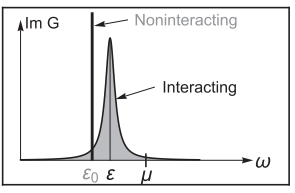
\includegraphics[scale=0.7]{figs/1p_Green_function_interacting/interacting_regime_spectral_function_one.png} }}
    \qquad
    \subfloat[\centering ]{{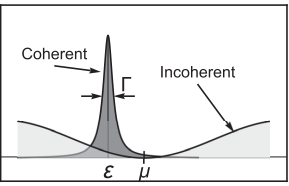
\includegraphics[scale=0.7]{figs/1p_Green_function_interacting/interacting_regime_spectral_function_two.png}}}
    \caption{\small Fig. A: Spectral function for a particle in a non-interacting system (black delta function) and of the corresponding quasiparticle after turning on interactions (gray filled curve). Notice the shift in energy and the linewidth broadening. \\
    Fig. B: Typical spectral function for a quasiparticle displaying its coherent component and the coherent background. } 
    \label{figs:1p_Green_f_(in)coh}
\end{figure}

Naturally, the full spectral function may be written as $ \mathcal{A}^{+}({\bf k}, \omega) = \mathcal{A}^{+}_{\textnormal{coh}}({\bf k}, \omega) +  \mathcal{A}^{+}_{\textnormal{incoh}}({\bf k}, \omega) $, which is schematically represented in \cref{figs:1p_Green_f_(in)coh}. The contributions from the coherent terms appear as a Lorentzian line shape, while the background arises from the incoherent part. If the quasiparticle weight vanishes, then the background only manifests itself in the spectral function. \\

The coherent terms of the spectral function have the following features:

\begin{enumerate}
    \item It has a Lorentzian profile peaked at $\varepsilon({\bf k})$. 
    \item The single-particle energies are renormalized, $\varepsilon_0 ({\bf k}) \rightarrow \varepsilon ({\bf k})$. 
    \item Its width is given by the inverse of the lifetime. 
    \item Its magnitude is proportional to the quasiparticle weight $\mathcal{Z}$, a positive number between 0 and 1. 
    \item The area under the peak has decreased, from $1$ and $\mathcal{Z}$.
\end{enumerate}

The incoherent terms, in contrasst, presents a continuum, not a peak. It must be present if $\mathcal{Z} \neq 1$, in order to satisfy the sum rule/normalization of the spectral function. A similar result is obtained for the hole spectral function, wherein $\Gamma < 0$. \\

\begin{tcolorbox}[colback=yellow, 
title = Physical Context]

Fermionic systems for which the previously laid picture holds are called Fermi liquids, its theory phenomenologically developed by Landau (1957), and in the subsequent years a microscopic formulation with the help of many-body perturbation theory was developed as well. \\

The identification and investigation of interacting fermionic systems which do not obey Fermi liquid theory is an important research area in modern many-body physics. Such non-Fermi liquids have, by definition, spectral functions which cannot be approximated by \cref{Fermi_liquids_valid_approx} and, therefore, cannot be understood in terms of a picture of non-interacting fermions. A prominent example of a non-Fermi liquid is the so-called Luttinger fermions, which occur in one-dimension.  
\end{tcolorbox}

\subsection{\textbf{Quantum Field Theory and Feynmann Rules}}

\paragraph{\textit{Perturbation theory and Feynmann Diagrams}}

In the definition of the Green function, the average values is taken with respect to the Heisenberg ground-state vector, $\ket{\psi_H}$, which is time-independent and very complicated for interacting systems, and no exact solution is achievable. The strategy is to set 

$$
    \ket{\psi_H} = \ket{\psi_I (0)} = \mathcal{S}^\dagger(t,0) \ket{\psi_I (t)},
$$

and use the time $t \rightarrow -\infty$ to interpolate the non-interacting ground state with the aid of the principle of adiabatic switching on. \\

\paragraph{The concept of Adiabaticity in Quantum Mechanics} \\

The construct of adiabaticity plays an important role in quantum many-body theory, by paving a path to understand a many-body problem, even when there is only an approximate solution. \\

In order to examine the usefulness of adibaticity, consider a many-body quantum system with Hamiltonian ${\bf H} = {\bf H}_0 + {\bf H}$, for which no exact solution of its ground state $\ket{\Psi_g}$ can be obtained but the exact ground state for ${\bf H}_0$, labelled as $\ket{\Phi_g}$, is known. To connect the two systems, the ${\bf H}_0$-Hamiltonian is ever present, with ground state $\ket{\Phi_g}$, and adiabatically slowly turn on ${\bf H}'$ until the total Hamiltonian is reached. This can be done by setting 

\begin{equation}
    {\bf H}(t) = {\bf H} + \lambda(t) {\bf H}', \textnormal{ where } \lambda(t) = e^{-\eta |t|} \textnormal{ and } \eta > 0, \textnormal{ is arbitrary small, }
    \label{Adiabatic_switching_on}
\end{equation}

\begin{figure}
    \centering
    \subfloat[\centering ]{{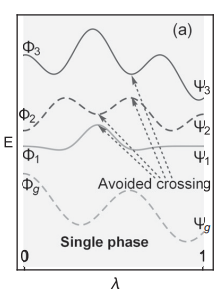
\includegraphics[scale=0.8]{figs/1p_Green_function_interacting/adiabatic_evol_no_phase_tr.png} }}
    \qquad
    \subfloat[\centering ]{{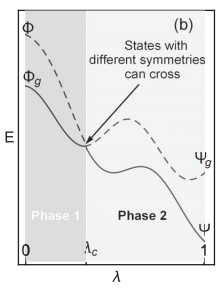
\includegraphics[scale=0.8]{figs/1p_Green_function_interacting/adiabatic_evol_phase_tr.png}}}
    \caption{\small  Fig a): Adiabatic evolution of a discrete spectrum within the symmetry subspace of the ground state. The ground state can be adiabatically evolved all the way to $\lambda = 1$, from $\ket{\Phi_g}$ to $\ket{\Psi_g}$. Fig b): Adiabatic evolution of the Hilbert space with $\lambda$. A phase transition occurs at $\lambda = \lambda_c$, where an excited state of the unperturbed Hamiltonian, with a symmetry different from that of the ground state, crosses below the ground state. } 
    \label{figs:adiabatic_evols}
\end{figure}

and varying $-\infty \leq t \rightarrow 0$. The efficacy of this approach hinges on whether $\ket{\Phi_g}$ has the same basic symmetries as $\ket{\Psi_g}$, ie. if these share the same quantum number labels. There are two possible paths for an adiabatic switching of a many-body system, diagramatically shown in figure \cref{figs:adiabatic_evols}:

\begin{enumerate}
    \item \textit{The ground-state symmetry remains invariant throughout the adiabatic evolution, } as $\lambda$ increases from 0 to 1. In such cases, the corresponding evolution of the energy spectrum, within the symmetry subspace of the ground state. In \cref{figs:adiabatic_evols}, subfigure a), a discrete spectrum with a series of avoided crossing, from $\lambda = 0$ to $\lambda = 1$, is shown. These crossings are avoided since the states have the same symmetries. The avoided crossing arise since an intersection of two levels having the same symmetry is removed because, in general, the off-diagonal matrix elements between the two states will not vanish, and thus will give rise to mutual repulsion. 
    \item \underline{The ground-state symmetry changes during the evolution due to a crossing of}
    
    \underline{ an energy level with different symmetry}, as shown in \cref{figs:adiabatic_evols}, subfigure b). In this case, it is possible for the energy levels of states with different symmetries to cross, since selection rules give vanishing matrix elements between the states, and thus prevent them from mixing. This scenarios leads to an adiabatic evolution, where a level crossing actually occurs at some $\lambda = \lambda_c$. Within such scenario, and excited state $\ket{\Phi}$ of the unperturbed Hamiltonian, with a symmetry different from that of the ground state $\ket{\Psi_g}$, may cross at $\lambda_c$ to a lower energy than the ground state, resulting in a symmetry change of the ground state. A simple example is when a ferromagnetic ground state becomes stabilized by interactions, however, in this case a continuous rotational symmetry of the spin is broken (ie. spontaneous symmetry breaking).  \\ 
\end{enumerate}

Thus, the switching-on procedure may become troublesome. Specially if it leads to instabilities at some critical value $\lambda = \lambda_c$. The presence of a $\lambda_c$ ushers a phase transition whereby the ground state changes its symmetry. If the transition is non-analytic, it signals a quantum critical transition initiated at a quantum critical point. \\

In many cases of interesent, there is no symmetry-changing phase transition as the perturbation Hamiltonian is turned on, and the procedure of adiabatic evolution can be used to turn on the interaction and to analytically evolve the ground state from $\ket{\Phi_g}$ to $\ket{\Psi_g}$. The adiabatic concept, together with the Gell-Mann-Low theorem, are key elements to perturbation theory. \\

\paragraph{Gell-Mann-Low Theorem}

\blanky \\

\begin{tcolorbox}[colback = LimeGreen, title = Historical Context]

In a 1951 seminal paper, Murray Gell-Mann and Francis Low used the adiabatic construct to establish the connection between the interacting and non-interacting Green functions, in the famous Gell-Mann-Low theorem. 

\end{tcolorbox}

The ground state $\ket{\Psi_0}$, which appears in the definition of the Green function of the interacting system, must be a time independent state in the Heisenberg picture. So far, only expectation values about the non-interacting ground state $\ket{\Phi_0}$ can be calculated. Thus, a path is needed to connect the states of the exactly solvable unperturbed Hamiltonian ${\bf H}_0$ with the ones of the full Hamiltonian. For this purpose, consider the time-dependent Hamiltonian given by \cref{Adiabatic_switching_on}, which allows for the adiabatic switching on:

\begin{itemize}
    \item For $|t|\rightarrow \infty$, the Hamiltonian reduces to ${\bf H}_0$. 
    \item At $t=0$, it becomes the interacting problem of interest.
    \item In the $\eta \rightarrow 0$-limit, the interaction is switched on adiabatically.
\end{itemize}

The scattering operator, in this context, is thus defined as 

\begin{equation}
    \mathcal{S}_{\eta}(t, t_0) = \sum_{n = 0}^{\infty} \frac{1}{n!} (-i)^{n} \int_{t_0}^{t} dt_1 \cdots \int_{t_0}^{t} dt_n \blanky e^{-\eta (|t_1| + \cdots + |t_n|)} \mathcal{T} [{\bf H}_{I}(t_1) \cdots {\bf H}_{I}(t_n)].
\end{equation}

As $t_0 \rightarrow - \infty$, the effect of the interaction vanishes and the problem reduces to that of the unperturbed Hamiltonian, 

$$
    t_0 \rightarrow -\infty \Longleftrightarrow \left\{\begin{array}{cc}
         {\bf H}_0 \ket{\Psi_0} = E^{(0)} \ket{\Psi_0}  \\
         \ket{\Psi_I(t_0)} \rightarrow \ket{\Psi_0}. 
    \end{array}\right.
$$

Now, recall the relation among state vector in different pictures, 

$$
    \ket{\Psi_H} = \ket{\Psi_S(t=0)} = \ket{\Psi_I (t=0)},
$$

where $t=0$ corresponds to the fully interacting Hamiltonian. In particular, the following relation between the Heisenberg and interaction state vectors is found 

$$
    \ket{\Psi_H} = \ket{\Psi_I (0)} = \mathcal{S}_{\eta}(0, - \infty) \ket{\Psi_0}. 
$$

The previous equation gives the relationship between the eigenstates of the non-interacting system with those of the fully interacting one, albeit via the adiabatic switching process. Then, the following theorem arises \\

\begin{theorem} \textbf{\textnormal{Gell-Mann-Low theorem}}

In the absence of any symmetry breaking transition, and in the $(\eta \rightarrow 0)$-limit, $\mathcal{S}_{\eta} \rightarrow \mathcal{S}_I$, and provides the right solution. To be more precise, let $\ket{\Psi_0}$ be an eigenstate of the unperturbed Hamiltonian ${\bf H_0}$ with energy $E^{(0)}$, and consider the interacting Hamiltonian given by

$$
    {\bf H} = {\bf H} + g e^{-\eta |t|} {\bf H}',
$$

which effectively interpolates between ${\bf H}$ and ${\bf H}_0$ in the limit $\eta \rightarrow 0$ and $|t|\rightarrow 0$. Let $\mathcal{S}_{\eta}$ denote the evolution operator in the interaction limit. Then, in the $(\eta \rightarrow 0)$-limit,

$$
    \ket{\Psi_{\eta}^{(\pm)}} = \frac{\mathcal{S}(0, \pm\infty) \ket{\Psi_0}}{\bra{\Psi_0} \mathcal{S}(0, \pm\infty) \ket{\Psi_0}},
$$

exists, is well defined with the $ \ket{\Psi_{\eta}^{(\pm)}}$-states being the eigenstates of the full Hamiltonian.

\end{theorem}

\begin{proof}

In effect, let the coupling constant be $g = e^{\eta \theta}$ and consider the Dyson expansion of the evolution operator. From Schr\"odinger's equation for the time evolution operator, it is known that 

$$
    i \partial_{t_1} \mathcal{S}_{\eta}(t_1,t_2) = {\bf H} \mathcal{S}_{\eta}(t_1,t_2), \textnormal{ with } \mathcal{S}_{\eta}(t_2,t_2) = \textnormal{id}, 
$$

and the adjoint Schr\"odinger equation establishes that 

$$
-i \partial_{t_1} \mathcal{S}_{\eta}(t_1,t_2) = \mathcal{S}_{\eta}(t_1,t_2) {\bf H}(t_1). 
$$

Then, formally 

$$
    \mathcal{S}_{\eta}(t_1,t_2) = \textnormal{id} - i \int_{t_2}^{t_1}dt' \blanky ({\bf H}_0 + e^{-\eta (|t'| - \theta)} {\bf H}') \mathcal{S}_{\eta}(t',t_2).
$$


Then, for $t_2 \leq t_1 \leq 0$ and with $\tau = t' + \theta$, it follows that 

\begin{equation}
    \begin{split}
        \mathcal{S}_{\eta}(t_1,t_2) = \textnormal{id} - i \int_{\theta + t_2}^{\theta + t_1}dt' \blanky ({\bf H}_0 + e^{\eta \tau} {\bf H}') \mathcal{S}_{\eta}(\tau - \theta,t_2) \\
        \Rightarrow \partial_{\theta} \mathcal{S}_{\eta}(t_1,t_2) \equiv \eta \partial_{g} \mathcal{S}_{\eta}(t_1,t_2) =& \partial_{t_1} \mathcal{S}_{\eta}(t_1,t_2) + \partial_{t_2}\mathcal{S}_{\eta}(t_1,t_2) \\
        &= {\bf H}(t_1) \mathcal{S}_{\eta}(t_1,t_2) - \mathcal{S}_{\eta}(t_1,t_2) {\bf H}(t_2).
    \end{split}
    \label{Gell_Mann_Low}
\end{equation}

The corresponding equation in the interaction picture can be obtained from the previous equation by pre-multiplying both sides with $e^{i {\bf H} t_1}$ and post-multiplying with $e^{i {\bf H} t_2}$ and using the definition of the interaction picture, namely that 

$$
    \mathcal{S}_{\eta, I}(t_1,t_2) = e^{i {\bf H_0} t_1} \mathcal{S}_{\eta}(t_1,t_2) e^{i {\bf H_0} t_2}. 
$$

The other case, in which $t_2 \geq t_1 \geq 0$, can be obtained in a similar fashion, yielding an additional global minus sign in front of the commutator. The mixed-sign case is not of interest here. Then, using the definition of the $\ket{\Psi_{\eta}^{(\pm)}}$ and employing \cref{Gell_Mann_Low}

\begin{equation}
    \begin{split}
        &\bigg({\bf H}_{\eta}(t=0) - E_0 \pm i \eta g \partial_{g} \bigg) \mathcal{S}_{\eta, I}(0,\pm \infty) \ket{\Psi_0} = 0. \\
        &\Rightarrow \mp i \eta g \partial_{g} \mathcal{S}_{\eta, I}(0,\pm \infty) \ket{\Psi_{\eta}^{(\pm)}}= ({\bf H}_{\eta} - E_0)  \mathcal{S}_{\eta, I}(0,\pm \infty) \ket{\Psi_{\eta}^{(\pm)}}\\
        &\Rightarrow \mp i \eta g \partial_{g} \ket{\Psi_0}= \frac{({\bf H} - E_0) \mathcal{S}_{\eta}(t_1,t_2) \ket{\Psi_0} }{ \bra{\Psi_0} \mathcal{S}_{\eta}(t_1,t_2) \ket{\Psi_0}} - \frac{\mathcal{S}_{\eta}(t_1,t_2) \ket{\Psi_0}}{ \bra{\Psi_0} \mathcal{S}_{\eta}(t_1,t_2) \ket{\Psi_0}} \bra{\Psi_0} ({\bf H} - E_0) \mathcal{S}_{\eta}(t_1,t_2) \ket{\Psi_0}  \\
\\
\Rightarrow \mp i \eta g \partial_{g} \ket{\Psi_0} &= ({{\bf H}} - E_0) \ket{\Psi_{\eta}^{(\pm)}} -  \bra{\Psi_{\eta}^{(\pm)}} \bra{\Psi_0} {{\bf H}} - E_0  \ket{\Psi_{\eta}^{(\pm)}} \\
&= [{{\bf H}} -\mathcal{E}^{(\pm)}] \ket{\Psi_{\eta}^{(\pm)}},
    \end{split}
\end{equation}

where $\mathcal{E}^{(\pm)} = E_0 + \bra{\Psi_0} {{\bf H}} - {{\bf H}}_0  \ket{\Psi_{\eta}^{(\pm)}}$. In the $\eta \rightarrow 0^+$-limit, by assumption, $g \partial_{g} \ket{\Psi_{\eta}^{(\pm)}}$ is finite. Then, it is clear that $\ket{\Psi_{\eta}^{(\pm)}}$ is an eigenstate of the full Hamiltonian, completing the proof. 

\end{proof}

\blanky \\

\paragraph{One-particle Green functions as a power series in the interaction}

The Gell-Mann-Low theorem connects the eigenstates of the non-interacting system with those of the fully interacting one, with the aid of the interaction picture. The Heisenberg operators, appearing in the Green function, remain to be related to those in the corresponding interaction picture. \\

To that end, consider the relationship between operators in the Heisenberg and interaction pictures,

\begin{equation}
    {\bf O}_{H}(t) = e^{i {\bf H} t} {\bf O}_{S} e^{-i {\bf H} t} = e^{i {\bf H} t} e^{-i {\bf H}_0 t} {\bf O}_{I} e^{i {\bf H}_0 t} e^{-i {\bf H} t}.
\end{equation}

Furthermore, the states in the interaction picture are given by 

\begin{equation}
    \ket{\Psi_I(t)} = e^{i{\bf H}_0 t} e^{-i {\bf H}t} \ket{\Psi_I(0)} = \mathcal{S}_{I}(t,0) \ket{\Psi_I(0)}.
\end{equation}

Then, 

\begin{equation}
    {\bf O}_{H}(t) = \mathcal{S}_{I}(0,t) {\bf O}_{I}(t) \mathcal{S}_{I}(t,0). 
\end{equation}

With these ingredients, the product of two Heisenberg operators, in the interaction picture, reads

\begin{equation}
    \begin{split}
        {\bf O}_{H}(t) {\bf O}_{H}(t_1) =& \mathcal{S}_{I}(0,t) {\bf O}_{I}(t) \mathcal{S}_{I}(t,0)  \mathcal{S}_{I}(0,t_1) {\bf O}_{I}(t_1) \mathcal{S}_{I}(t_1,0) \\
        &= \mathcal{S}_{I}(0,t) {\bf O}_{I}(t) \mathcal{S}_{I}(t,t_1) {\bf O}_{I}(t_1) \mathcal{S}_{I}(t_1,0).
    \end{split}
\end{equation}

Then, the Green function in terms of interaction-picture operators reads

\begin{equation}
\begin{split}
    i \mathfrak{G}(x; x') &= \bra{\Psi_H} \mathcal{T} [\psi_{H}(x) \psi^\dagger_{H}(x')] \ket{\Psi_H} \\
    &= \frac{\bra{\Phi_0} \mathcal{S}_I(\infty, 0) \mathcal{T} [\mathcal{S}_I(0, t) \psi_{I}(x) \mathcal{S}_I(t, t') \psi_{I}(x') \mathcal{S}_I(t', 0) ] \mathcal{S}_I(0, -\infty)\ket{\Phi_0}}{\bra{\Phi_0} \mathcal{S}_I(\infty, 0)\mathcal{S}_I(0, -\infty)\ket{\Phi_0}},
\end{split}
\end{equation}

where $x \equiv ({\bf x}, t, \sigma)$ for compactness. The $(\psi_H, \psi_H^\dagger)$-Heisenberg operators have been replaced by their interaction-picture conterparts, which simply evolve under the action of the unperturbed Hamiltonian ${\bf H}_0$. The ground state of the interaction problem $\ket{\Psi_0}$ has been replaced by the non-interacting one, $\ket{\Phi_0}$. Furthermore, since the evolution operations $\mathcal{S}$ form a semigroup, all evolution operators in the preceding equation can be combined into a single $\mathcal{S}$, for the time-ordering operator takes care of the proper time ordering anyhow, thus yielding 

\begin{equation}
\begin{split}
     i \mathfrak{G}^{\sigma \sigma'}({\bf x}, t; {\bf x}', t') &= \frac{\bra{\Phi_0}  \mathcal{T} [\mathcal{S}_I(-\infty, \infty) \psi_{I \sigma}({\bf x}, t)\psi_{I \sigma'}({\bf x}', t')]\ket{\Phi_0}}{\bra{\Phi_0} \mathcal{S}_I(\infty, -\infty)\ket{\Phi_0}} \\
     &= \sum_{n=0}^{\infty} \frac{1}{n!} (-i)^n \int_{-\infty}^{\infty} dt_1 \cdots \int_{-\infty}^{\infty} dt_n \blanky \frac{\bra{\Phi_0} \mathcal{T} [{\bf H}_{I}(t_1) \cdots {\bf H}_{I}(t_n) \psi_{I \sigma}({\bf x}, t)\psi_{I \sigma'}({\bf x}', t')]\ket{\Phi_0}}{\bra{\Phi_0} \mathcal{S}_I(\infty, -\infty)\ket{\Phi_0}},
\end{split}
\end{equation}

where the one-particle Green function is now explicitly written as an expansion in powers of the perturbation ${\bf H}_I$. For this reformulation to be useful, a method is needed to mitigate taking expectation values of large numbers of operators in a non-interacting sytem. This procedure is systematized with the application of Wick's theorem and simplified with the aid of Feynmann diagrams. \\

\paragraph{\textit{Wick's Theorem: Normal ordering and contractions}}

In the preceding identity for the one-particle Green function, the arraying of interaction Hamiltonians is fixed by time ordering. However, as the interaction Hamiltonian contains creation and annihilation operators, it is convenient to move all annihilation operators to the right, where these can eliminate particles. This ordering is called the \textit{normal ordering}. Furthermore, observables have zero-expectation values in the vacuum state, it is convenient to construct them in normal order, with creation operators on the left of destruction operators. Wick's theorem provides a way to go from time-ordered to normal-ordered products, which is valid when the expectation values are with respect to a Hamiltonian that is quadratic in fermionic (bosonic) operators. \\

Recall from the study of superfluidity phenomenom that the Bogoliubov canonical transformation generated new non-interacting quasiparticles from the original interacting bosons, and the emerging ground state acted as a vacuum state for the new quasiparticles. 
In many physical situations, the ground state $\ket{\Psi_g}$, of some incipient effective Hamiltonian, will be taken to be the reference vacuum state. Such a state is filled with both particles and quasiparticles, and the effective Hamiltonian is expressed in a basis of canonical operators $\bigg\{({\bm \alpha}_{a}, {\bm \alpha}^\dagger_{a})\bigg\}_{a = 1}$, where 

\begin{align}
    {\bm \alpha}_{a} \ket{\Psi_g} &= 0, & \bra{\Psi_g} {\bm \alpha}_{a}^\dagger = 0,
\end{align}

where this action only holds for such systems, but not for the other creation and annihilation operators associated with the system. \\

\begin{tcolorbox}[colback = yellow, title = Physical Context]

In order to bring light upon these ideas, consider the non-interacting ground state $\ket{\Phi_0}$, describing the Fermi sea. Then, the field operators are given in terms of the canonical particle-hole transformation,

\begin{equation}
    \psi({\bf x}) = \sum_{{\bf k} \sigma} \phi_{{\bf k} \sigma} {\bf c}_{{\bf k} \sigma} = \left\{\begin{array}{cc}
       \sum_{{\bf k} \sigma} \phi_{{\bf k} \sigma}({\bf x}) {\bf d}_{{\bf k} \sigma} = \phi^{(-)}({\bf x}) & \textnormal{ if $k > k_F$ annihilates particles}{} \\
       \sum_{{\bf k} \sigma} \phi_{{\bf k} \sigma}({\bf x}) {\bf h}_{-{\bf k} \sigma} = \phi^{(+)}({\bf x}) & \textnormal{ if $k < k_F$ create holes }{}
    \end{array}\right.,
\end{equation}

then 

\begin{align}
    \phi^{(-)}({\bf x}) \ket{\Phi_0} &= 0, & \phi^{(+)^\dagger}({\bf x}) \ket{\Phi_0} &= 0.
\end{align}

The preceding relations indicate that $(\phi^{(-)}, \phi^{(+)\dagger})$ are annihilation parts, while $(\phi^{(+)}, \phi^{(-)\dagger})$ are the creation operators. 

\end{tcolorbox}

The following discussion will be restricted to 
fermionic operators in a non-interacting system. 

\begin{definition}

Consider a product of operators ${\bf A}_i^{\pm}$ is normally ordered if all the ${\bf A}_i^{-}$-operators are on the right of the ${\bf A}_i^{+}$-operators, i.e.

$$
    {\bf A}_1^{+} \cdots {\bf A}_k^{+} {\bf A}_1^{-} \cdots {\bf A}_n^{-}.
$$

\end{definition}

The usefulness of this definition is that the expectation value on the ground state of a normally ordered operator product is always zero. \\

It is clear that any product of operators ${\bf A}_1 \cdot {\bf A}_n$ can be written as a sum of normally ordered terms. In effect, every local operator can be written as ${\bf A}_i^{+} + {\bf A}_i^{-}$, thus yielding $2^n$ terms. In each term, the components ${\bf A}_i^{-}$ are brought to the right by succesive anticommutation, yielding the desired result. Wick's theorem is an efficient answer to this particular problem: to write a product $\prod_{i} {\bf A}_i$ as a sum of normally ordered terms. The theorem is an extremely useful operator identity, with important corollaries. \\

\begin{definition}[Normal Ordering]
    The normal-ordering operator, $\bm{\mathcal{N}}$ brings a generic product into a normal form. If a product of operators contains $k$ ${\bf A}_i^+$-factors mixed with $n-k$ ${\bf A}^-_i$-factors, it action is given by 
    
    \begin{equation}
        \bm{\mathcal{N}} [{\bf A}_i^{(\pm)} \cdots {\bf A}_n^{(\pm)}] = (\pm 1)^{P} {\bf A}_{i_1}^{+} \cdots {\bf A}_{i_k}^{+} \cdots {\bf A}_{i_n}^{-}, 
    \end{equation}
    
    where $P$ is the permutation which brings the $(1, \cdots,n)$-sequence to its normal ordered $(i_1, \cdots, i_n)$-sequence. \\
\end{definition}

At first glance, it may seem that the normal ordering is ambiguous, since the (+)-operators and $(-)$-operators can be given in different orders. However, the different expressions are actually the same operator, since ${\bf A}^+$-operators anticommute among themselves, with the same being true for the ${\bf A}^-$-operators. For example, $\bm{\mathcal{N}}[{{\bf A}_1^+ {\bf A}_2^+}] = {{\bf A}_1^+ {\bf A}_2^+} = - {{\bf A}_2^+ {\bf A}_1^+}$. Now, any product $\prod_i {\bf A}_i$ can be written as a sum of normally ordered terms. 

\begin{tcolorbox}[colback = Bittersweet, title = Example]

Consider for example a product of two operators, 

\begin{equation}
    \begin{split}
        {\bf A}_1 {\bf A}_2 &= ({\bf A}_1^+ + {\bf A}_1^-)({\bf A}_2^+ + {\bf A}_2^-) \\
        &= {\bf A}_{1}^{+} {\bf A}_{2}^{+} + {\bf A}_{1}^{-} {\bf A}_{2}^{+} + {\bf A}_{1}^{+} {\bf A}_{2}^{-} + {\bf A}_{1}^{-} {\bf A}_{2}^{-} \\
        &= \bm{\mathcal{N}} [{\bf A}_1 {\bf A}_2] + \{{\bf A}_1^-, {\bf A}_2^+\}.
    \end{split}
\end{equation}

The vanishing of the expectation value of a normally ordered product implies 

\begin{equation}
    \{{\bf A}_1^-, {\bf A}_2^+\} = \bra{\Psi_g} {\bf A}_1 {\bf A}_2 \ket{\Psi_g},
\end{equation}

which is a c-number, the \underline{contraction} of the two operators, denoted ${\bf A}_1^c {\bf A}_2^c$. 

\end{tcolorbox}

Using the previous example:

\begin{definition}[Contraction]
     
    The contraction of two operators, where a product of $n'$ operators is inserted between them, may be defined by 
    
    \begin{equation}
        {\bf A}_1^c ({\bf A}_{1'} \cdots {\bf A}_{n'}) {\bf A}_2^c = (-1)^{n'}   {\bf A}_1^c {\bf A}_2^c ({\bf A}_{1'} \cdots {\bf A}_{n'}).
    \end{equation}
     
\end{definition}

Wick's theorem provides a computationally efficient way for calculating operator contractions, by mapping it to a purely combinatorial problem. 

\begin{theorem}Wick's theorem \\

Consider a product of $n$ operators, then the following equality holds:

\begin{equation}
    {\bf A}_1 \cdots {\bf A}_n = \bm{\mathcal{N}}[1\cdots n] + \sum_{c} \bm{\mathcal{N}}[\cdots i^c \cdots j^c \cdots n] + \sum_{c, d} \bm{\mathcal{N}}[\cdots i^c \cdots r^d \cdots j^c \cdots s^d \cdots n] + \cdots,
\end{equation}

where the first sum is performed over single contractions of pairs, the second sum is performed over double contractions and so on. If $n$ is even, the result consists only of products of contractions (c-numbers).

\end{theorem}

Some important consequences of Wick's theorem readily follow, 

\begin{remark}
    As a general rule, the expectation value of a product of destruction and creation operators. Particle number conservation thus requieres that the number of destruction operators equals that of creators.
\end{remark}

\begin{corr}

The following identity can be proved from Wick's theorem\footnote{

\begin{tcolorbox}[colback = Bittersweet, title = Example]

Using the previous corollary, it is trivial that 

\begin{equation}
    \bra{\Psi_g} 1234 \ket{\Psi_g} = \langle 12 \rangle \langle 34 \rangle - \langle 13 24 \rangle + \langle 14 \rangle \langle 23 \rangle.
\end{equation}

\end{tcolorbox}

},

\begin{equation}
    \bra{\Psi_g} {{{\bf A}}}_1 \cdots {{\bf A}}_{2n} \ket{\Psi_g} = \sum_{\mathcal{P}_2} (-1)^{P} \langle {{\bf A}}_{i_1} {{\bf A}}_{j_1} \rangle \cdots \langle {{\bf A}}_{i_n} {{\bf A}}_{j_n} \rangle, {\begin{array}{cc}
         \textnormal{ where the sum is performed over the set $\mathcal{P}_2$ of}  \\
         \textnormal{ partitions of $1, \cdots, 2n$ into sets of } \\
         \textnormal{ pairs $\{(i_1, j_1), \cdots, (i_n, j_n)\}$ with $(i,j) \sim (j,i)$} \\
         \textnormal{ belonging to the same equivalency class.}
    \end{array}}
\end{equation}

\end{corr}

\blanky \\
An important variation of Wick's theorem deals with the normal-ordering of a time-ordered product, via a $\bm{\mathcal{T}}$-contraction operator. 

\begin{theorem}

Consider a product of two-operators. Then, its time-ordered product can be written as 

\begin{equation}
    \mathcal{T} {{\bf A}}_{i}(t_i) {{\bf A}}_{j}(t_j) = \bm{\mathcal{N}}[{{\bf A}}_{i}(t_j) {{\bf A}}_{j}(t_i)] + \overbrace{{{\bf A}}_{i}(t_i) {{\bf A}}_{j}(t_j)}, 
\end{equation}

then a $\bm{\mathcal{T}}$(time ordered)-contraction is defined as 

\begin{equation}
    \overbrace{{{\bf A}}_{i}(t_i) {{\bf A}}_{j}(t_j)} = \bra{\Psi_g} \mathcal{T} {{\bf A}}_{i}(t_i) {{\bf A}}_{j}(t_j) \ket{\Psi},
\end{equation}

\end{theorem}

\begin{remark}
    The $\bm{\mathcal{T}}$-contraction of two-operators is such that 
    
    \begin{equation}
        \overbrace{{{\bf A}}_{i}(t_i) (\cdots ) {{\bf A}}_{j}(t_j)} = (-1)^k \overbrace{{{\bf A}}_{i}(t_i) {{\bf A}}_{j}(t_j)} ()\cdots).
    \end{equation}
\end{remark}

\begin{remark}
    The $\bm{\mathcal{T}}$-contractions have a new property, not shared by ordinary contractions,
    
    \begin{equation}
        \overbrace{{{\bf A}}_{i}(t_i) {{\bf A}}_{j}(t_j)} = - \overbrace{{{\bf A}}_{j}(t_j) {{\bf A}}_{i}(t_i)}.
    \end{equation}
\end{remark}

\begin{remark}

From the previous definitions and remarks, the following explicit expressions can be given, 

\begin{equation} \begin{split}
    \overbrace{\psi(t_1) \psi^\dagger(t_2)} =& \bigg \langle \mathcal{T} \psi(t_1) \psi^\dagger(t_2) \bigg \rangle \\
    &= i \mathfrak{G}^{(0)}(1,2)
\end{split}, \blanky \blanky \blanky \blanky \begin{split}
    \overbrace{\psi(t_1) \psi(t_2)} =& \bigg \langle \mathcal{T} \psi(t_1) \psi(t_2) \bigg \rangle \\
    &= i \mathfrak{F}^{(0)}(1,2)
\end{split}, \blanky \blanky \blanky \blanky \begin{split}
    \overbrace{\psi^\dagger(t_1) \psi^\dagger(t_2)} =& \bigg \langle \mathcal{T} \psi^\dagger(t_1) \psi^\dagger(t_2) \bigg \rangle \\
    &= i \mathfrak{F}^{(0)\dagger}(1,2).
\end{split}
\end{equation}
    
\end{remark}

For systems where $\ket{\Psi_g}$ has a definite number of particles, the anomalous correlators $\mathfrak{F}^{(0)}, \mathfrak{F}^{(0)\dagger}$ are zero. They are non-zero, for example, in the Bardeen-Cooper-Schrieffer theory. \\

\subsubsection{\textbf{Feynmann Diagrams}}

\clearpage

\section{Linear Response Theory}

Linear response theory is an extremely widely used concept in physics, stating that the response to a weak external perturbation is proportional to the perturbation, and therefore the quantity of interest is the proportionality constant. The physical question to ask is thus: supposing some perturbation $H'$, what is the measured consequence for an observable quantity ${\bf A}$. In other words, what is $\langle {\bf A} \rangle$ to linear order in $H'$? 

Among the numerous physical application of the linear response formalism, one can mention charge and spin susceptibilities of eg. electron systems due to external electric or magnetic fields. Responses to external mechanical forces or vibrations can also be calculated using the same formalism. \\

\paragraph{\textbf{The general Kubo formula}}

Consider a quantum system described by a time independent Hamiltonian ${\bf H}_0$ in thermodynamic equilibrium. This means that an expectation value of a physical quantity, described by the operator ${\bf A}$, which can be evaluated as 

\begin{equation}
    \begin{split}
        \langle {\bf A} \rangle = \frac{1}{\mathcal{Z}_0} \textnormal{Tr }_{\mathds{H}} \rho_0 {\bf A}  = \frac{1}{\mathcal{Z}_0} \sum_{n \in \Lambda} \bra{n} {{\bf A}} \ket{n} e^{-\beta E_n} \\
        \rho_0 = e^{-\beta {\bf H}_0} = \sum_{n \in \Lambda} \ket{n} \bra{n} e^{-\beta E_n},
    \end{split} \begin{array}{c}
         \textnormal{ where $\{\ket{n}\}_{n \in \Lambda}$ is a complete} \\
         \\
         \textnormal{set of eigenstates}.
    \end{array}
\end{equation}

Suppose now that at some time, $t = t_0$, an external perturbation is applied to the system, driving it out of equilibrium. The perturbation is described by an additional time dependent term in the Hamiltonian 

\begin{equation}
    \Hamiltonian(t) = \Hamiltonian_0 + \Hamiltonian'(t) \theta(t-t_0)
\end{equation}

Now, the interest lies in finding the expectation value of the ${\bf A}$ operator at times $t$ greater that $t_0$-. In order to do so, the time evolution of the density matrix must be found, or equivalently the time evolution of the eigenstates of the unperturbed Hamiltonian. Once $\ket{n(t)}$ is found, the time-dependent expectation value can be found as 

\begin{align}
        \langle {\bf A}(t) \rangle = \frac{1}{\mathcal{Z}_0} \textnormal{Tr }_{\mathds{H}} \rho(t) {\bf A}  = \frac{1}{\mathcal{Z}_0} \sum_{n \in \Lambda} \bra{n(t)} {{\bf A}} \ket{n(t)} e^{-\beta E_n} \\
        \rho_0 = e^{-\beta {\bf H}_0} = \sum_{n \in \Lambda} \ket{n(t)} \bra{n(t)} e^{-\beta E_n},
\end{align}

The physical idea behind this expression is as follows. The initial states of the system are distributed according to the usual Boltzmann distribution $\frac{e^{-\beta E_{0n}}}{\mathcal{Z_0}}$. At later times, the system is described by the same distribution of states but the states are now time-dependent and they have evolved according to the new Hamiltonian. The time dependence of the states $\ket{n(t)}$ is governed by the Schr\"odinger equation. Since $\Hamiltonian'$ is regarded to be a small perturbation, the interaction picture representation is suitable for this setting. In this representation, the time dependence is given by 

\begin{equation}
    \ket{n(t)} = e^{-i\Hamiltonian_0 t} \ket{n(t)}_I = e^{-i\Hamiltonian_0 t} \mathcal{U}(t, t_0) \ket{\hat{n}(t_0)},
\end{equation}

where by definition $\ket{\hat{n}(t_0)} = e^{i \Hamiltonian_0 t_0} \ket{n(t_0)} = \ket{n}$.

Up to linear order in $\Hamiltonian'$, the time evolution operator $\mathcal{U}(t, t_0)$ can be written 

$$
    \mathcal{U}(t, t_0) = \mathds{1} - i \int_{t_0}^t dt' \Hamiltonian'(t') + \mathcal{O}(\Hamiltonian^{'2})
$$

Then, using this in the time-dependent expectation value yields 

\begin{equation} \begin{split}
    \langle {\bf A}(t) \rangle &= \frac{1}{\mathcal{Z}_0} \sum_{n \in \Lambda} \bra{n(t)} {{\bf A}} \ket{n(t)} e^{-\beta E_n} \\
    &= \frac{1}{\mathcal{Z}_0} \sum_{n \in \Lambda} \bra{n(t_0)} \bigg(\mathds{1} - i \int_{t_0}^t dt' \Hamiltonian'(t')\bigg) e^{-i \Hamiltonian_0 t_0} {{\bf A}} e^{i \Hamiltonian_0 t_0} \bigg(\mathds{1} - i \int_{t_0}^t dt' \Hamiltonian'(t')\bigg) \ket{n(t_0)}  e^{-\beta E_n}+ \mathcal{O}(\Hamiltonian^{'2}) \\
    &= \frac{1}{\mathcal{Z}_0} \sum_{n \in \Lambda} \bra{n(t_0)} {{\bf A}} \ket{n(t_0)} - \frac{i}{\mathcal{Z}_0} \int_{t_0}^{t} dt' \sum_{n \in \Lambda} e^{-\beta E_n} \bigg( e^{-i \Hamiltonian_0 t_0} {{\bf A}} e^{i \Hamiltonian_0 t_0} \Hamiltonian'(t') - \Hamiltonian'(t')e^{-i \Hamiltonian_0 t_0} {{\bf A}} e^{i \Hamiltonian_0 t_0} \ket{n(t_0)} \bigg) \\
    &= \langle {{\bf A}} \rangle_{0} + \int_{t_0}^{t} \frac{dt'}{i} \langle[{{\bf A}}(t), \Hamiltonian'(t')]\rangle_{0},
\end{split}
\end{equation}

where the brackets $\langle \rangle_{0}$ means an equilibrium average with respect to the Hamiltonian $\Hamiltonian$. This is in fact a remarkable and very useful result since the inherently non-equilibrium quantity $\langle {{\bf A}}(t) \rangle$ has been expressed as a correlation function of the system in equilibrium. The physical reason for this is that the interaction between excitations created in the non-equilibrium state is an effect to second order in the weak perturbation, hence not included in the linear response. \\

The correlation function is the retarded correlation function, which can be rewritten as 
the difference between $\langle {{\bf A}}(t) \rangle \textnormal{ and } \langle {{\bf A}}\rangle_0 $ ie. 

\begin{align} 
        & \alignedbox{\delta \langle {{\bf A}}(t) \rangle }{
        = \int_{t_0}^{\infty} dt' \mathcal{C}_{AH'}^{R}(t,t') e^{-\eta(t-t')} \textnormal{ where } \mathcal{C}_{AH'}^{R}(t,t') = -i \theta(t-t') \langle[{{\bf A}}(t), \Hamiltonian'(t')]\rangle_{0}},
\end{align}

which is the Kubo formula. This expresses the linear response to a perturbation $\Hamiltonian'$. Note that the factor $e^{-\eta(t-t')}$, with an infinitesimal positive parameter $\eta$, has been included to force the response at time $t$ due to the influence of $\Hamiltonian'$ at time $t'$ to decay when $t >> t'$. At the end of the calculation, the limit $\eta \rightarrow 0^+$,. This is so since the retarded effect of a perturbation must decrease in time\footnote{The other, the advanced correlation function is non-physical and must be ditched. The other one, the retarded correlation function, decreases exponentially with time, the exponential factor thus picks out the physically relevant solution by introducing an artificial relaxation mechanism.}. \\

\paragraph{\textbf{Kubo fromula in the frequency domain}}

It is often convenient to express the response to an external disturbance in the frequency domain via Fourier transformations\footnote{Consider the $L^1$-space, ie. the space of all integrable functions on the real line. Then the Fourier transform and the Fourier-anti transform can be defined as 
\begin{align}
    \mathcal{F}[f(t)](\omega) = f(\omega) = \int_{\R} dt e^{i\omega t} f(t) \blanky \textnormal{ and } \blanky \mathcal{F}^{-1}[f(\omega)](t) = f(t) = \int_{\R} \frac{d\omega}{2\pi} e^{-i\omega t} f(\omega)
\end{align}

}. Therefore, consider the perturbation Hamiltonian $\Hamiltonian'$, which can be rewritten in terms of its Fourier components 

\begin{equation}
    \Hamiltonian'(t) = \int_{\Omega \subset \R} \frac{d\omega}{2\pi} e^{-i\omega t} \Hamiltonian'_\omega,
\end{equation}

such that the retarded correlation function becomes 

\begin{equation}
    \mathcal{C}_{AH'}^{R}(t,t') = \int_{\mathds{R}} \frac{d\omega}{2\pi} e^{-i\omega t'} \mathcal{C}_{AH'_\omega}^{R}(t-t') \begin{array}{c}
         \textnormal{since $\langle[{{\bf A}}(t), \Hamiltonian'(t')_{\omega'}]\rangle_{0}$ only depends } \\
         \textnormal{ on the difference between $t$ and $t'$. }
    \end{array}
\end{equation}

Therefore, inserting this result into the Kubo formula yields

\begin{equation}
    \begin{split}
        \delta \langle {{\bf A}}(t) \rangle
        &= \int_{t_0}^{\infty} dt' \mathcal{C}_{AH'_\omega}^{R}(t,t') e^{-\eta(t-t')} \\
        &= \int_{\R} dt' \int_{\R} \frac{d\omega}{2\pi} e^{-i\omega t} e^{-i(\omega + i\eta) (t'-t)} \mathcal{C}_{AH'_\omega}^{R}(t-t') \\
        &= \int_{\R} \frac{d\omega}{2\pi} e^{-¿i\omega t} \bigg(\int_{\R} d(t'-t) e^{-i(\omega + i\eta)(t'-t)} \mathcal{C}_{AH'_\omega}^{R}(t-t')\bigg) \\
        &= \int_{\R} \frac{d\omega}{2\pi} e^{-i\omega t} \mathcal{C}_{AH'_\omega}^{R}(\omega; \eta) 
    \end{split}
\end{equation}

which can be inverted to yield the final result in the frequency domain

\begin{equation}
    \begin{split}
        \int_{\R} {dt} e^{i\nu t}
        \delta \langle {{\bf A}}(t) \rangle &= \int_{\R} {dt} e^{i\nu t} \int_{\R} \frac{d\omega}{2\pi} e^{-i\omega t} \mathcal{C}_{AH'_\omega}^{R}(\omega; \eta) \\
        \langle {{\bf A}}_\nu \rangle &= \int_{\R} \frac{d\omega}{2\pi} \int_{\R} dt e^{i(\nu - \omega)t} \mathcal{C}_{AH'_\omega}^{R}(\omega; \eta) \\
        &= \int_{\R} {d\omega} \delta(\nu - \omega) \mathcal{C}_{AH'_\omega}^{R}(\omega; \eta) \\
        &= \mathcal{C}_{AH'_\nu}^{R}(\nu; \eta) 
    \end{split}
\end{equation}

\begin{align}
       & \alignedbox{\Rightarrow \delta \langle {{\bf A}}_\omega \rangle = \mathcal{C}_{AH'_\omega}^{R}(\omega) \textnormal{ with } \mathcal{C}_{AH'_\omega}^{R}(\omega)}{ = \int_{\R} dt e^{i\omega t} e^{-\eta t} \mathcal{C}_{AH'_\omega}^{R}(t)},
\end{align}

{where the infinitesimal $\eta$ parameter is incorporated } { in order to ensure the correct physical result, ie.} {the retarded response function decays at $t>>1$.} \\

\paragraph{\textbf{Kubo formula for conductivity}}

Consider a system of charged particles, eg. electrons, which is subjected t an external electromagnetic field. The electromagnetic field induces a current and the conductivity is the linear response coefficient. In the general case, the conductivity is a non-local quantity in both time and space, such that the electric current ${{\bf J}_e}$ at some point ${\bf x}$ at time $t$ depends on the electric field at points ${\bf y}$ at times $t'$, eg.\footnote{Note that this section's mathematical treatment is not Lorentz-covariant. This is, the spacetime is treated as $\R^4$ with the metric being $g_{\mu \nu} = \delta_{\mu \nu}$} 

\begin{equation}
    J^{\alpha}_{e}(x^\mu) = \int_{\Omega \subset \R^4 } dx^{\mu} \sum_{\alpha \beta} \sigma_{\beta}(x^\mu, y^{\mu}) E^{\beta} (y^{\mu}), \begin{array}{c} 
         \textnormal{ where $\sigma_{\alpha \beta}(x^\mu, y^{\mu})$ is the conductivity tensor, which  } \\ 
         \textnormal{ describes the current response in the } \\
         \textnormal{ ${\bf e}_\alpha$-direction to an applied }
         \textnormal{ electric field in the ${\bf e}_\beta$-direction.}
    \end{array}
\end{equation}

The electric field ${\bf E}$ is given by the electric potential $\phi_{ext}$ and the vector potential ${\bf A}_{\textnormal{ext}}$ as $
{\bf E}(x^\mu) = -\partial_{\mu} A^{\mu}$. For electrons, the current density can be written as ${\bf J}_e = -e \langle {\bf J} \rangle$. The perturbing term in the Hamiltonian due to the external electromagnetic field is given by the coupling of the electrons to both the scalar potential and the vector potential. Then, upto linear order in the external potential, 

$$
\Hamiltonian_{\textnormal{ext}} = -e \int_{\R^3} d{\bf x} J_{\mu}({\bf x}) A^{\mu}_{\textnormal{ext}}(x^{\mu}).
$$

Let, ${\bf A}_0$ denote the vector potential in the equilibrium ie. prior to the onset of the perturbation ${\bf A}_0(x^{\mu}$ and let ${\bf A}_0(x^{\mu})$ denote the total vector potential. Then, 

$$
   {\bf A}(x^{\mu}) = {\bf A}_{0}(x^{\mu}) +  {\bf A}_{\textnormal{ext}}(x^{\mu}).
$$

The current operator can be decomposed in two components, the diamagnetic and the paramagnetic terms, as follows 

\begin{equation}
    {\bf J} = {\bf J}^{\nabla}({\bf x}) + \frac{e}{m} {\bf A}({\bf x}) \rho({\bf x}).  
\end{equation}

For simplicity and using gauge invariance, the external electric potential can be set to zero. The conductivity is most easily expressed in the frequency domain via a Fourier transformation of the perturbation. Since 

\begin{equation} \begin{array}{cc}
     \partial_t \overset{\mathcal{F}}{\rightarrow} -i\omega \blanky & \textnormal{ then } \blanky {\bf A}_{\textnormal{ext}}({\bf x}, \omega) \overset{\mathcal{F}}{\rightarrow}  \frac{1}{i\omega} {\bf E}_{\textnormal{ext}}({\bf x}, \omega) \\
\end{array}
     \Rightarrow \Hamiltonian_{\textnormal{ext}, \omega} = \frac{e}{i\omega} \int_{\Omega \subset \R^3} d{\bf x} \blanky {\bf J}({\bf x}) \cdot {\bf E}_{\textnormal{ext}}({\bf x}, \omega).
\end{equation}

In order to exploit the frequency domain formulation of linear response theory, it is desirable to find the corresponding formula for the conductivity tensor in frequency-space. The conductivity tensor is a property of the equilibrium system and can thus onyly depend on time differences $ \sigma_{\alpha \beta}(x^\mu, y^{\mu}) =  \sigma_{\alpha \beta}({\bf x},{\bf y}, t-t')$. The frequency transform of the conductivity yields

\begin{equation}
    J^{\alpha}_{e}({\bf x}, \omega) = \int_{\Omega \subset \R^3 } d{\bf y} \blanky \sum_{ \beta} \sigma_{\alpha \beta}({\bf x},{\bf y}, \omega) E^{\beta}({\bf y}, \omega).
\end{equation}

Now, given that he external perturbation, written in frequency space, is already linear in the external potential ${\bf E}_{\textnormal{ext}}$, and given that the interest lies only on terms proportional to said perturbation, the conductivity can be rewritten as 

\clearpage

\section{Microscopic Theory of Conventional Superconductivity}

From \textbf{Advanced Quantum Condensed Matter Physics, One-Body, Many-Body and Topological perspectives. Michael El-Batanouny} \\

\paragraph{\textbf{}}



\bibliography{citations.bib}
\bibliographystyle{abbrv}
\end{document}

